\chapter{Appendix}\label{ch:appAlabel}

\section{Terminology table}

%\begin{tabular}{}

\begin{table}[ht]
    \begin{tabular}{| p{0.29\linewidth} | p{0.5\linewidth}| p{0.15\linewidth}|}
        \hline
        \textbf{Term}           & \textbf{Definition}                                                       & \textbf{Source} \\ \hline
        Software entity         & Software that is to be characterized by measuring its attributes.         & FEETINGS\cite{MANCEBO2021100558}        \\ \hline
        Software entity class   & The collection of all the entities that satisfy the determined objective. & FEETINGS        \\ \hline
        Test Case               & A representation of functionality of the software entity to be measured.  & FEETINGS        \\ \hline
        Test Case Measurement    & A set of energy consumption measurements of all the runs in a test case.  & FEETINGS        \\ \hline
        Measurement             & A set of energy consumption record taken by a measuring instrument.       & FEETINGS        \\ \hline
        Samples                 & Each energy consumption record taken by a measuring instrument.           & FEETINGS        \\ \hline
        Device Under Test (DUT) & A device where the software entity to be measured is run.                 & FEETINGS        \\ \hline
        Measuring Instrument    & A method used to make energy consumption measurements.                    & FEETINGS        \\ \hline
        Setup                   & A defined step of procedures executes at DUT startup.                     & R3\cite{Bokhari2020r3}              \\ \hline
        Batch                   & A set of test cases executed in sequence with a cool of periods.            & NEW             \\ \hline
    
    \end{tabular}
    \caption{Terminology used throughout the are report.}
    \label{tab:feetTable}
    \end{table}
\newpage

\section{CPU-states}\label{app:CPU_states}
 What is presented here is largely based on information from Intel\cite{CIntel} and some sources that convey the material in a more presentable manner \cite{CMete,CLinux}. The C-states manage how the system consumes energy, C0 is the normal operation of a working computer under load. Each incremental C-State shuts more of the CPU down until at C10 it is nearly completely shut down. Different CPUs and motherboards could however support a different amount of c-states. The same idea applies to CC-States(Core C-states), PC-States(Package C-States) in addition to the Thread C-States and Hyper-Thread C-States, but the information on these is very sparse. Some CPUs also have enhanced C-States (C1E) able to shut more of the CPU down, but not enough to be the next C-State. The P-States are only used during C0, where they control the frequency of the CPU under load to better manage its energy usage. S-States (Sleep State) controls how the system is using energy, but on a larger scale as it controls if the system is sleeping or not. Every C-States occur within S0, while increments define deeper states of sleep such as Sleep and Hibernation. The G-States (Global-States) define the overall state of the system such as G0 being a working computer where S0, C-States and P-States can occur and G3 when the DUT is completely shut down. The expectation based on this is that since the problem only seemed to occur during the idle experiments we suspected it had something to do with the C-states.
\newpage

\section{Results: Timeseries}

\input{tabels/reulsts_timeseries/Workstation_IntelPowerGadget}

\begin{figure}[ht]  
    \centering 
    \begin{subfigure}[b]{0.49\linewidth}
        \begin{tikzpicture}
            \pgfplotsset{%
        width=1\linewidth,
        % height=1\textheight
            }
            \begin{axis}[ymax=120,
                            xlabel={Time (Seconds)},
                            ylabel={Energy Consumption (Joules)},
                            ]
                            \addplot[color=blue, mark=none,] coordinates { %% AVG value
                            (0.0, 0.0)(0.1001669449081803, 14.503508083333333)(0.2003338898163606, 14.831769499999998)(0.3005008347245409, 13.989308500000005)(0.4006677796327212, 14.069865166666672)(0.5008347245409015, 14.189435999999999)(0.6010016694490818, 14.293162166666658)(0.7011686143572621, 14.025847166666667)(0.8013355592654424, 14.191664916666667)(0.9015025041736228, 14.23757908333334)(1.001669449081803, 14.31203566666667)(1.1018363939899833, 14.114125416666669)(1.2020033388981637, 14.317239416666666)(1.3021702838063438, 14.109161083333328)(1.4023372287145242, 14.26197141666666)(1.5025041736227045, 14.198953916666673)(1.6026711185308848, 14.115162416666667)(1.7028380634390652, 14.296757166666662)(1.8030050083472455, 14.144347666666665)(1.9031719532554257, 14.226744499999999)(2.003338898163606, 14.213088166666672)(2.1035058430717863, 14.202346333333333)(2.2036727879799667, 14.311400666666662)(2.303839732888147, 14.348520166666672)(2.4040066777963274, 14.196476083333332)(2.5041736227045073, 14.257923250000005)(2.6043405676126876, 14.256809583333341)(2.704507512520868, 14.129653499999996)(2.8046744574290483, 14.225218333333327)(2.9048414023372287, 14.313160166666668)(3.005008347245409, 14.150227833333338)(3.1051752921535893, 14.256280666666669)(3.2053422370617697, 14.28319158333333)(3.30550918196995, 14.320463916666666)(3.4056761268781304, 14.135349916666664)(3.5058430717863107, 14.399936999999998)(3.606010016694491, 14.302301)(3.7061769616026714, 14.273182499999999)(3.8063439065108513, 14.359327416666662)(3.906510851419032, 14.164433499999998)(4.006677796327212, 14.360152333333337)(4.106844741235393, 14.136692333333336)(4.207011686143573, 14.374979249999996)(4.3071786310517535, 14.204720749999996)(4.407345575959933, 14.317519249999997)(4.507512520868114, 14.231688916666663)(4.607679465776294, 14.274245000000006)(4.707846410684475, 14.265786749999998)(4.808013355592655, 14.360980750000001)(4.908180300500835, 14.12106291666667)(5.0083472454090145, 14.463271)(5.108514190317195, 14.103183749999998)(5.208681135225375, 14.329035083333332)(5.308848080133556, 14.322025250000001)(5.409015025041736, 14.22842825000001)(5.509181969949917, 14.304782666666659)(5.609348914858097, 14.336603)(5.709515859766277, 14.224848000000001)(5.809682804674457, 14.259185000000002)(5.909849749582638, 14.351012166666662)(6.010016694490818, 14.265933916666672)(6.110183639398999, 14.205799249999997)(6.210350584307179, 14.388955750000001)(6.3105175292153595, 14.196959833333343)(6.410684474123539, 14.277962916666665)(6.510851419031719, 14.163990999999994)(6.6110183639399, 14.151544749999998)(6.71118530884808, 14.283161666666667)(6.811352253756261, 14.22629683333333)(6.911519198664441, 14.371647333333332)(7.011686143572621, 14.246219749999996)(7.111853088480801, 14.263462500000001)(7.212020033388982, 14.265487083333337)(7.312186978297162, 14.28997658333333)(7.412353923205343, 14.269250499999998)(7.512520868113523, 14.29538866666667)(7.612687813021703, 14.258753250000002)(7.712854757929884, 14.289717500000005)(7.813021702838064, 14.311679666666672)(7.913188647746244, 14.248320833333333)(8.013355592654424, 14.228260500000008)(8.113522537562606, 14.312986916666661)(8.213689482470786, 14.26412375)(8.313856427378965, 14.305779999999997)(8.414023372287145, 14.217131999999994)(8.514190317195327, 14.236988583333341)(8.614357262103507, 14.316939499999993)(8.714524207011687, 14.273954666666668)(8.814691151919867, 14.369145249999999)(8.914858096828048, 14.369648166666668)(9.015025041736228, 14.178847000000001)(9.115191986644408, 14.300383333333327)(9.215358931552588, 14.308196666666664)(9.31552587646077, 14.370903750000002)(9.41569282136895, 14.274555749999998)(9.51585976627713, 14.358529666666664)(9.61602671118531, 14.326241833333341)(9.71619365609349, 14.185592166666664)(9.81636060100167, 14.401960916666669)(9.916527545909851, 14.522078083333332)(10.016694490818029, 14.08612508333334)(10.11686143572621, 14.338927)(10.21702838063439, 14.391620166666668)(10.31719532554257, 14.324726916666672)(10.41736227045075, 14.398843416666665)(10.51752921535893, 14.22928775)(10.617696160267112, 14.350675916666667)(10.717863105175292, 14.37714033333333)(10.818030050083472, 14.309330416666665)(10.918196994991652, 14.471937583333332)(11.018363939899833, 14.122999999999996)(11.118530884808013, 14.329456749999995)(11.218697829716193, 14.360218249999996)(11.318864774624373, 14.399179249999998)(11.419031719532555, 14.31735108333333)(11.519198664440735, 14.267216166666666)(11.619365609348915, 14.432320499999998)(11.719532554257095, 14.205504583333322)(11.819699499165276, 14.272908166666666)(11.919866444073456, 14.361621750000003)(12.020033388981636, 14.338082666666658)(12.120200333889816, 14.294569583333338)(12.220367278797998, 14.263996916666663)(12.320534223706177, 14.293623999999998)(12.420701168614357, 14.328591583333331)(12.520868113522537, 14.39769816666667)(12.621035058430719, 14.393024916666668)(12.721202003338899, 14.246153833333336)(12.821368948247079, 14.355340333333332)(12.921535893155259, 14.301950249999999)(13.021702838063439, 14.254297333333323)(13.12186978297162, 14.475767499999996)(13.2220367278798, 14.361230416666672)(13.32220367278798, 14.344201250000005)(13.42237061769616, 14.377857333333326)(13.522537562604342, 14.255818000000003)(13.622704507512521, 14.291492499999993)(13.722871452420701, 14.316369833333335)(13.823038397328881, 14.278863166666667)(13.923205342237063, 14.4353525)(14.023372287145243, 14.252074499999999)(14.123539232053423, 14.280369083333325)(14.223706176961603, 14.234567166666666)(14.323873121869784, 14.299402166666665)(14.424040066777964, 14.362140750000005)(14.524207011686144, 14.42481358333333)(14.624373956594324, 14.300312333333336)(14.724540901502506, 14.366952249999999)(14.824707846410686, 14.367858416666671)(14.924874791318866, 14.362612749999991)(15.025041736227045, 14.357609249999992)(15.125208681135225, 14.160450249999995)(15.225375626043405, 14.48053358333334)(15.325542570951589, 14.276554083333334)(15.425709515859769, 14.347614916666663)(15.525876460767948, 14.351886833333328)(15.626043405676128, 14.384881499999999)(15.726210350584308, 14.321878249999996)(15.826377295492488, 14.449466416666668)(15.926544240400668, 14.379856166666668)(16.026711185308848, 14.326979833333331)(16.126878130217026, 14.408603166666666)(16.22704507512521, 14.319075916666664)(16.32721202003339, 14.36996808333333)(16.42737896494157, 14.271579999999998)(16.52754590984975, 14.461623249999999)(16.62771285475793, 14.366020916666667)(16.72787979966611, 14.317697166666665)(16.82804674457429, 14.31812975)(16.92821368948247, 14.344232333333334)(17.028380634390654, 14.309721333333334)(17.128547579298832, 14.350905583333335)(17.228714524207014, 14.336363416666668)(17.328881469115192, 14.481398000000008)(17.429048414023374, 14.353565666666668)(17.529215358931552, 14.354576916666668)(17.629382303839733, 14.391824000000002)(17.72954924874791, 14.341964749999999)(17.829716193656097, 14.388791666666659)(17.929883138564275, 14.436548083333337)(18.030050083472457, 14.327172833333334)(18.130217028380635, 14.427666833333328)(18.230383973288816, 14.37878791666667)(18.330550918196995, 14.343347333333332)(18.430717863105176, 14.309457250000005)(18.530884808013354, 14.49000425)(18.63105175292154, 14.385008333333333)(18.731218697829718, 14.333393500000003)(18.8313856427379, 14.285567083333332)(18.931552587646078, 14.337741416666669)(19.03171953255426, 14.320485)(19.131886477462437, 14.483294666666673)(19.23205342237062, 14.380934666666668)(19.332220367278797, 14.339613999999994)(19.43238731218698, 14.464089833333333)(19.53255425709516, 14.398100333333334)(19.63272120200334, 14.425907166666672)(19.73288814691152, 14.497516083333334)(19.833055091819702, 14.352426000000003)(19.93322203672788, 14.322036083333339)(20.033388981636058, 14.514962083333335)(20.13355592654424, 14.272688916666665)(20.23372287145242, 14.266173333333343)(20.333889816360603, 14.599073083333339)(20.43405676126878, 14.337915333333331)(20.534223706176963, 14.356835749999993)(20.63439065108514, 14.37537483333333)(20.734557595993323, 14.347976)(20.8347245409015, 14.473997333333333)(20.934891485809683, 14.289143499999991)(21.03505843071786, 14.414946083333337)(21.135225375626046, 14.413018416666665)(21.235392320534224, 14.372308416666675)(21.335559265442406, 14.21544258333333)(21.435726210350584, 14.401192666666667)(21.535893155258766, 14.433562166666668)(21.636060100166944, 14.338220083333336)(21.736227045075125, 14.386494083333336)(21.836393989983303, 14.509789583333335)(21.93656093489149, 14.331394249999994)(22.036727879799667, 14.382114916666666)(22.13689482470785, 14.39626933333333)(22.237061769616027, 14.397098333333336)(22.33722871452421, 14.335265416666667)(22.437395659432386, 14.450615500000003)(22.537562604340568, 14.411981166666669)(22.637729549248746, 14.29266766666667)(22.737896494156928, 14.567121666666662)(22.83806343906511, 14.313673999999995)(22.93823038397329, 14.405170416666667)(23.03839732888147, 14.489749666666663)(23.13856427378965, 14.359831916666673)(23.23873121869783, 14.358981416666674)(23.33889816360601, 14.512414416666664)(23.43906510851419, 14.368407416666663)(23.53923205342237, 14.309350166666674)(23.639398998330552, 14.335631166666664)(23.739565943238734, 14.378991249999997)(23.839732888146912, 14.338936750000006)(23.939899833055094, 14.480025166666668)(24.040066777963272, 14.368030916666667)(24.140233722871454, 14.458891249999999)(24.24040066777963, 14.438058416666665)(24.340567612687813, 14.401422416666662)(24.440734557595995, 14.419162666666663)(24.540901502504177, 14.556949)(24.641068447412355, 14.37596525)(24.741235392320537, 14.459232166666672)(24.841402337228715, 14.41486958333334)(24.941569282136896, 14.401497916666665)(25.041736227045075, 14.43798716666666)(25.141903171953256, 14.464608333333336)(25.242070116861438, 14.369755083333335)(25.34223706176962, 14.411192750000007)(25.442404006677798, 14.483925666666668)(25.54257095158598, 14.395990000000008)(25.642737896494157, 14.38193075)(25.74290484140234, 14.565209750000006)(25.843071786310517, 14.39407708333333)(25.9432387312187, 14.436151250000005)(26.043405676126877, 14.400734749999998)(26.143572621035062, 14.409834249999998)(26.24373956594324, 14.420684083333331)(26.34390651085142, 14.345300416666678)(26.4440734557596, 14.518455999999997)(26.544240400667782, 14.38159566666667)(26.64440734557596, 14.375014499999999)(26.744574290484138, 14.520993833333334)(26.84474123539232, 14.465020666666662)(26.9449081803005, 14.455681916666672)(27.045075125208683, 14.523649833333335)(27.14524207011686, 14.365289083333336)(27.245409015025043, 14.443652666666672)(27.34557595993322, 14.458560583333343)(27.445742904841403, 14.283604249999996)(27.54590984974958, 14.46911491666667)(27.646076794657763, 14.404092166666663)(27.746243739565944, 14.470244333333337)(27.846410684474126, 14.358717333333336)(27.946577629382304, 14.410022916666673)(28.046744574290486, 14.389840249999995)(28.146911519198664, 14.379545333333336)(28.247078464106846, 14.468764416666657)(28.347245409015024, 14.361682749999995)(28.447412353923205, 14.49070608333333)(28.547579298831387, 14.417626250000001)(28.64774624373957, 14.323256916666676)(28.747913188647747, 14.474358833333332)(28.84808013355593, 14.471956833333333)(28.948247078464107, 14.450032)(29.04841402337229, 14.421986083333334)(29.148580968280466, 14.424843583333335)(29.248747913188648, 14.445509500000005)(29.348914858096826, 14.515241750000001)(29.44908180300501, 14.41159425000001)(29.54924874791319, 14.32444758333334)(29.64941569282137, 14.479637916666665)(29.74958263772955, 14.418425000000001)(29.84974958263773, 14.423531749999995)(29.94991652754591, 14.496158333333337)(30.05008347245409, 14.42993566666667)(30.15025041736227, 14.473228833333335)(30.25041736227045, 14.518447)(30.35058430717863, 14.36943433333334)(30.45075125208681, 14.359688583333334)(30.55091819699499, 14.484358583333337)(30.651085141903177, 14.453566166666665)(30.751252086811355, 14.52255566666667)(30.851419031719537, 14.498193250000003)(30.951585976627715, 14.402566333333334)(31.051752921535897, 14.42210758333333)(31.151919866444075, 14.495584083333325)(31.252086811352257, 14.371529333333333)(31.352253756260435, 14.457065499999999)(31.452420701168617, 14.459638833333338)(31.552587646076795, 14.394688416666664)(31.652754590984976, 14.345574500000007)(31.752921535893154, 14.457320333333325)(31.853088480801336, 14.584511250000004)(31.953255425709514, 14.37492216666666)(32.053422370617696, 14.506518916666671)(32.15358931552588, 14.448323249999993)(32.25375626043405, 14.419151583333342)(32.35392320534224, 14.338612)(32.45409015025042, 14.45022425)(32.554257095158604, 14.475579750000003)(32.65442404006678, 14.39244966666667)(32.75459098497496, 14.533669499999997)(32.85475792988314, 14.432503666666666)(32.95492487479132, 14.594343583333332)(33.0550918196995, 14.464659833333327)(33.15525876460768, 14.43103341666667)(33.25542570951586, 14.52963141666666)(33.35559265442404, 14.42034725)(33.45575959933222, 14.361809999999998)(33.5559265442404, 14.42399958333333)(33.65609348914858, 14.514723583333332)(33.756260434056756, 14.471265916666672)(33.85642737896494, 14.488478333333322)(33.95659432387313, 14.392068833333338)(34.05676126878131, 14.423164666666672)(34.15692821368948, 14.536060999999997)(34.257095158597664, 14.451230750000006)(34.357262103505846, 14.60848308333333)(34.45742904841403, 14.398014666666661)(34.5575959933222, 14.52461025)(34.657762938230384, 14.454212249999994)(34.757929883138566, 14.407916583333337)(34.85809682804675, 14.50699225)(34.95826377295492, 14.56326691666667)(35.058430717863104, 14.335142583333331)(35.158597662771285, 14.458174833333327)(35.25876460767947, 14.47546191666667)(35.35893155258764, 14.425164583333338)(35.45909849749582, 14.449425916666664)(35.559265442404005, 14.388039666666668)(35.659432387312194, 14.610716083333333)(35.75959933222037, 14.389403416666669)(35.85976627712855, 14.410262083333333)(35.95993322203673, 14.541364333333325)(36.06010016694491, 14.483798583333336)(36.16026711185309, 14.436206666666658)(36.26043405676127, 14.438058750000005)(36.36060100166945, 14.481855583333328)(36.46076794657763, 14.444263333333332)(36.56093489148581, 14.558195749999994)(36.66110183639399, 14.442121666666658)(36.76126878130217, 14.48109275)(36.86143572621035, 14.452304583333335)(36.96160267111853, 14.546461166666665)(37.06176961602671, 14.561333833333334)(37.16193656093489, 14.476083249999995)(37.26210350584308, 14.470192666666664)(37.362270450751254, 14.431431750000002)(37.462437395659435, 14.476158083333337)(37.56260434056762, 14.500477500000008)(37.6627712854758, 14.509066833333323)(37.76293823038397, 14.52309508333333)(37.863105175292155, 14.523369916666667)(37.96327212020034, 14.433872083333334)(38.06343906510852, 14.459669583333328)(38.16360601001669, 14.496148083333338)(38.263772954924875, 14.440249916666664)(38.363939899833056, 14.542077666666673)(38.46410684474124, 14.483818833333336)(38.56427378964941, 14.43397925)(38.664440734557594, 14.465742333333335)(38.764607679465776, 14.477161333333335)(38.86477462437396, 14.542056916666667)(38.96494156928214, 14.441328666666664)(39.06510851419032, 14.4948255)(39.1652754590985, 14.602684833333338)(39.26544240400668, 14.46999483333334)(39.36560934891486, 14.443423750000001)(39.46577629382304, 14.566109500000005)(39.56594323873122, 14.484674083333333)(39.666110183639404, 14.48345783333333)(39.76627712854758, 14.438704083333329)(39.86644407345576, 14.5529005)(39.96661101836394, 14.467095749999993)(40.066777963272116, 14.415246583333333)(40.1669449081803, 14.511329916666671)(40.26711185308848, 14.502368749999992)(40.36727879799666, 14.473962166666665)(40.46744574290484, 14.472314166666667)(40.567612687813025, 14.579156333333332)(40.667779632721206, 14.42723933333333)(40.76794657762939, 14.486199416666667)(40.86811352253756, 14.595085249999993)(40.968280467445744, 14.477715999999992)(41.068447412353926, 14.456815749999995)(41.16861435726211, 14.526946000000002)(41.26878130217028, 14.514291083333326)(41.368948247078464, 14.458799333333326)(41.469115191986646, 14.603117083333332)(41.56928213689483, 14.3906595)(41.669449081803, 14.604062999999993)(41.769616026711184, 14.379352916666669)(41.869782971619365, 14.43654233333333)(41.96994991652755, 14.577232916666667)(42.07011686143572, 14.475294999999994)(42.1702838063439, 14.510705)(42.27045075125209, 14.456790500000006)(42.370617696160274, 14.446806250000002)(42.47078464106845, 14.456923499999997)(42.57095158597663, 14.497750750000003)(42.67111853088481, 14.470548583333331)(42.77128547579299, 14.532906666666669)(42.87145242070117, 14.432417249999999)(42.97161936560935, 14.591820499999999)(43.07178631051753, 14.556928916666664)(43.17195325542571, 14.423287499999995)(43.27212020033389, 14.600192833333331)(43.37228714524207, 14.475640166666663)(43.47245409015025, 14.492659083333342)(43.57262103505843, 14.555525666666673)(43.67278797996661, 14.483849583333336)(43.77295492487479, 14.583748499999993)(43.87312186978298, 14.49826883333333)(43.97328881469116, 14.51259758333333)(44.073455759599334, 14.492973500000002)(44.173622704507515, 14.499566999999994)(44.2737896494157, 14.443789750000004)(44.37395659432388, 14.511625833333325)(44.47412353923205, 14.527270833333336)(44.574290484140235, 14.485131500000003)(44.67445742904842, 14.368127333333328)(44.7746243739566, 14.566867249999996)(44.87479131886477, 14.549030333333333)(44.974958263772955, 14.489779833333335)(45.075125208681136, 14.446257166666667)(45.17529215358932, 14.523043999999997)(45.27545909849749, 14.536676166666659)(45.375626043405674, 14.420734166666664)(45.475792988313856, 14.456439916666671)(45.57595993322204, 14.508924833333333)(45.67612687813022, 14.59888533333334)(45.7762938230384, 14.408175833333333)(45.87646076794658, 14.543313749999992)(45.976627712854764, 14.386478249999998)(46.07679465776294, 14.582842999999999)(46.17696160267112, 14.49838133333333)(46.2771285475793, 14.497948999999998)(46.37729549248748, 14.601652083333331)(46.47746243739566, 14.391356333333334)(46.57762938230384, 14.530403833333336)(46.67779632721202, 14.501066666666668)(46.7779632721202, 14.524117666666665)(46.87813021702838, 14.49957116666666)(46.97829716193656, 14.492954166666664)(47.07846410684474, 14.548923)(47.17863105175292, 14.358418000000002)(47.278797996661105, 14.47978033333334)(47.378964941569286, 14.479495583333334)(47.47913188647747, 14.542570500000007)(47.57929883138564, 14.46642925)(47.679465776293824, 14.484123999999998)(47.779632721202006, 14.535496083333333)(47.87979966611019, 14.494642500000003)(47.97996661101836, 14.474938166666666)(48.080133555926544, 14.461617750000004)(48.180300500834726, 14.423231416666669)(48.28046744574291, 14.536278833333336)(48.38063439065108, 14.415286916666666)(48.48080133555926, 14.459267833333334)(48.580968280467445, 14.470910583333334)(48.68113522537563, 14.426796416666665)(48.7813021702838, 14.528349333333335)(48.88146911519199, 14.44995508333333)(48.98163606010017, 14.490004250000004)(49.081803005008354, 14.521131666666667)(49.18196994991653, 14.522021999999998)(49.28213689482471, 14.352298916666664)(49.38230383973289, 14.516854583333334)(49.48247078464107, 14.521655333333323)(49.58263772954925, 14.531253666666665)(49.68280467445743, 14.528730500000002)(49.78297161936561, 14.582217916666666)(49.88313856427379, 14.38658525)(49.98330550918197, 14.507775250000002)(50.08347245409015, 14.497674333333329)(50.18363939899833, 14.483692083333342)(50.28380634390651, 14.498594666666667)(50.38397328881469, 14.433114166666666)(50.484140233722876, 14.431740833333334)(50.58430717863106, 14.475996833333337)(50.68447412353924, 14.416934750000003)(50.784641068447414, 14.49823383333333)(50.884808013355595, 14.419920166666666)(50.98497495826378, 14.509509750000003)(51.08514190317196, 14.481189833333337)(51.18530884808013, 14.509239833333332)(51.285475792988315, 14.542061999999994)(51.3856427378965, 14.4437395)(51.48580968280468, 14.424782499999996)(51.58597662771285, 14.564426666666666)(51.686143572621035, 14.469602833333333)(51.786310517529216, 14.476103083333335)(51.8864774624374, 14.409051000000007)(51.98664440734557, 14.46107383333333)(52.086811352253754, 14.51282091666666)(52.18697829716194, 14.546537916666665)(52.287145242070125, 14.549751916666668)(52.3873121869783, 14.503685666666664)(52.48747913188648, 14.537036666666662)(52.58764607679466, 14.50797883333334)(52.68781302170284, 14.611162833333333)(52.78797996661102, 14.473230500000001)(52.8881469115192, 14.528639250000001)(52.98831385642738, 14.610685333333326)(53.088480801335564, 14.544467749999999)(53.18864774624374, 14.428211083333338)(53.28881469115192, 14.539060416666665)(53.3889816360601, 14.467197416666663)(53.489148580968276, 14.406090833333328)(53.58931552587646, 14.474587916666668)(53.68948247078464, 14.625013583333324)(53.78964941569283, 14.469501083333336)(53.889816360601, 14.503395999999997)(53.989983305509185, 14.610705999999997)(54.090150250417366, 14.480492749999998)(54.19031719532555, 14.503228499999999)(54.29048414023372, 14.560061750000001)(54.390651085141904, 14.37872783333333)(54.490818030050086, 14.516339333333345)(54.59098497495827, 14.544738000000006)(54.69115191986644, 14.563001083333331)(54.791318864774624, 14.470443000000008)(54.891485809682806, 14.529218166666668)(54.99165275459099, 14.584923750000003)(55.09181969949916, 14.530476000000004)(55.19198664440734, 14.571373416666667)(55.292153589315525, 14.44975166666666)(55.39232053422371, 14.522128500000004)(55.49248747913189, 14.58222308333333)(55.59265442404007, 14.432936333333336)(55.69282136894825, 14.48890483333333)(55.79298831385643, 14.61301524999999)(55.89315525876461, 14.510068833333337)(55.99332220367279, 14.592599166666664)(56.09348914858097, 14.555458999999997)(56.19365609348915, 14.575778583333339)(56.29382303839733, 14.53751916666667)(56.39398998330551, 14.472029333333332)(56.49415692821369, 14.579461250000001)(56.59432387312187, 14.529346083333335)(56.69449081803005, 14.57275724999999)(56.79465776293823, 14.461225666666675)(56.89482470784641, 14.511223749999997)(56.99499165275459, 14.526829166666671)(57.095158597662774, 14.58141383333333)(57.195325542570956, 14.516585083333341)(57.29549248747914, 14.571057999999999)(57.39565943238732, 14.430520666666673)(57.495826377295494, 14.408913833333335)(57.595993322203675, 14.602470999999992)(57.69616026711186, 14.529727333333332)(57.79632721202004, 14.492771500000007)(57.89649415692821, 14.450529083333345)(57.996661101836395, 14.558918083333326)(58.09682804674458, 14.482587500000001)(58.19699499165276, 14.50563)(58.29716193656093, 14.661980000000002)(58.397328881469114, 14.475279583333336)(58.497495826377296, 14.5261975)(58.59766277128548, 14.612801500000005)(58.69782971619365, 14.539462416666671)(58.79799666110184, 14.53855225)(58.89816360601002, 14.492089166666668)(58.9983305509182, 14.568022333333326)(59.09849749582638, 14.543841916666654)(59.19866444073456, 14.501097)(59.29883138564274, 14.486998249999996)(59.398998330550924, 14.592171583333334)(59.4991652754591, 14.531227666666672)(59.59933222036728, 14.58307191666667)(59.69949916527546, 14.668287749999998)(59.79966611018364, 14.58770066666667)(59.89983305509182, 14.61077233333333)(60.0, 14.456281583333338)
                            };
                            \addplot[color=blue, mark=none,name path=A] coordinates { %% MAX value
                            (0.0, 0.0)(0.1001669449081803, 20.13667)(0.2003338898163606, 17.01533)(0.3005008347245409, 16.654629999999997)(0.4006677796327212, 16.4056)(0.5008347245409015, 16.66744)(0.6010016694490818, 18.75117)(0.7011686143572621, 16.50569)(0.8013355592654424, 15.67807)(0.9015025041736228, 15.87032)(1.001669449081803, 16.20174)(1.1018363939899833, 15.70003)(1.2020033388981637, 15.87826)(1.3021702838063438, 15.59993)(1.4023372287145242, 15.46749)(1.5025041736227045, 16.05525)(1.6026711185308848, 15.568200000000001)(1.7028380634390652, 16.066860000000002)(1.8030050083472455, 15.45468)(1.9031719532554257, 16.06014)(2.003338898163606, 15.47115)(2.1035058430717863, 15.878870000000001)(2.2036727879799667, 15.72017)(2.303839732888147, 15.429649999999999)(2.4040066777963274, 15.39669)(2.5041736227045073, 16.03512)(2.6043405676126876, 16.36288)(2.704507512520868, 15.38814)(2.8046744574290483, 15.63045)(2.9048414023372287, 15.53829)(3.005008347245409, 15.74947)(3.1051752921535893, 15.708580000000001)(3.2053422370617697, 15.43148)(3.30550918196995, 15.7745)(3.4056761268781304, 15.657309999999999)(3.5058430717863107, 15.967970000000001)(3.606010016694491, 15.59261)(3.7061769616026714, 15.54806)(3.8063439065108513, 16.00582)(3.906510851419032, 16.02412)(4.006677796327212, 15.678669999999999)(4.106844741235393, 15.637170000000001)(4.207011686143573, 18.82258)(4.3071786310517535, 15.819049999999999)(4.407345575959933, 15.957609999999999)(4.507512520868114, 15.58651)(4.607679465776294, 15.47238)(4.707846410684475, 15.98079)(4.808013355592655, 15.55416)(4.908180300500835, 15.463830000000002)(5.0083472454090145, 16.01375)(5.108514190317195, 15.61702)(5.208681135225375, 15.95943)(5.308848080133556, 15.70857)(5.409015025041736, 15.92281)(5.509181969949917, 16.4947)(5.609348914858097, 16.663159999999998)(5.709515859766277, 15.82333)(5.809682804674457, 16.15658)(5.909849749582638, 17.35286)(6.010016694490818, 15.662799999999999)(6.110183639398999, 16.01681)(6.210350584307179, 15.759240000000002)(6.3105175292153595, 15.7806)(6.410684474123539, 15.80684)(6.510851419031719, 15.54378)(6.6110183639399, 15.69088)(6.71118530884808, 15.789150000000001)(6.811352253756261, 15.64449)(6.911519198664441, 16.03512)(7.011686143572621, 15.65914)(7.111853088480801, 15.45589)(7.212020033388982, 15.94723)(7.312186978297162, 16.20418)(7.412353923205343, 15.63839)(7.512520868113523, 15.85689)(7.612687813021703, 15.8392)(7.712854757929884, 15.503499999999999)(7.813021702838064, 15.72261)(7.913188647746244, 15.80623)(8.013355592654424, 15.26913)(8.113522537562606, 15.67623)(8.213689482470786, 16.01863)(8.313856427378965, 16.0992)(8.414023372287145, 15.71834)(8.514190317195327, 15.26913)(8.614357262103507, 15.3735)(8.714524207011687, 15.9399)(8.814691151919867, 16.15596)(8.914858096828048, 15.99971)(9.015025041736228, 15.87154)(9.115191986644408, 15.73422)(9.215358931552588, 15.92342)(9.31552587646077, 15.79891)(9.41569282136895, 15.51754)(9.51585976627713, 15.595049999999999)(9.61602671118531, 15.78304)(9.71619365609349, 16.40743)(9.81636060100167, 15.817829999999999)(9.916527545909851, 16.163899999999998)(10.016694490818029, 15.36984)(10.11686143572621, 15.946)(10.21702838063439, 15.714690000000001)(10.31719532554257, 15.8691)(10.41736227045075, 16.02718)(10.51752921535893, 15.51082)(10.617696160267112, 15.671949999999999)(10.717863105175292, 16.01131)(10.818030050083472, 15.728720000000001)(10.918196994991652, 16.7358)(11.018363939899833, 15.80257)(11.118530884808013, 15.66097)(11.218697829716193, 15.65426)(11.318864774624373, 16.56246)(11.419031719532555, 15.728100000000001)(11.519198664440735, 15.5389)(11.619365609348915, 15.99666)(11.719532554257095, 15.324670000000001)(11.819699499165276, 15.49801)(11.919866444073456, 15.54196)(12.020033388981636, 16.008869999999998)(12.120200333889816, 15.66707)(12.220367278797998, 15.73666)(12.320534223706177, 15.658529999999999)(12.420701168614357, 15.70797)(12.520868113522537, 15.745199999999999)(12.621035058430719, 15.90878)(12.721202003338899, 15.42964)(12.821368948247079, 15.70675)(12.921535893155259, 15.72933)(13.021702838063439, 16.11873)(13.12186978297162, 15.881920000000001)(13.2220367278798, 15.58651)(13.32220367278798, 15.807450000000001)(13.42237061769616, 15.63229)(13.522537562604342, 15.89047)(13.622704507512521, 15.68966)(13.722871452420701, 15.645109999999999)(13.823038397328881, 15.50411)(13.923205342237063, 16.20357)(14.023372287145243, 15.937460000000002)(14.123539232053423, 15.728720000000001)(14.223706176961603, 15.764119999999998)(14.323873121869784, 15.40401)(14.424040066777964, 15.54867)(14.524207011686144, 15.6921)(14.624373956594324, 15.85323)(14.724540901502506, 15.691489999999998)(14.824707846410686, 15.938680000000002)(14.924874791318866, 15.97041)(15.025041736227045, 16.09982)(15.125208681135225, 15.39547)(15.225375626043405, 16.05281)(15.325542570951589, 16.394)(15.425709515859769, 15.44246)(15.525876460767948, 15.94295)(15.626043405676128, 15.810500000000001)(15.726210350584308, 15.726890000000001)(15.826377295492488, 15.642050000000001)(15.926544240400668, 15.96126)(16.026711185308848, 16.032059999999998)(16.126878130217026, 15.84957)(16.22704507512521, 16.13216)(16.32721202003339, 16.09066)(16.42737896494157, 15.5328)(16.52754590984975, 15.568200000000001)(16.62771285475793, 15.64266)(16.72787979966611, 15.63534)(16.82804674457429, 15.61275)(16.92821368948247, 15.66769)(17.028380634390654, 16.55636)(17.128547579298832, 15.432699999999999)(17.228714524207014, 15.549280000000001)(17.328881469115192, 15.872150000000001)(17.429048414023374, 15.82271)(17.529215358931552, 15.96004)(17.629382303839733, 15.75984)(17.72954924874791, 15.50778)(17.829716193656097, 16.09188)(17.929883138564275, 15.76229)(18.030050083472457, 15.439419999999998)(18.130217028380635, 15.859939999999998)(18.230383973288816, 15.46749)(18.330550918196995, 15.34664)(18.430717863105176, 15.68722)(18.530884808013354, 15.93624)(18.63105175292154, 15.80441)(18.731218697829718, 15.68783)(18.8313856427379, 15.54806)(18.931552587646078, 16.177319999999998)(19.03171953255426, 15.678669999999999)(19.131886477462437, 15.951500000000001)(19.23205342237062, 15.926480000000002)(19.332220367278797, 15.85567)(19.43238731218698, 15.64632)(19.53255425709516, 15.4742)(19.63272120200334, 16.705280000000002)(19.73288814691152, 15.92587)(19.833055091819702, 15.69942)(19.93322203672788, 15.64754)(20.033388981636058, 16.115679999999998)(20.13355592654424, 15.70126)(20.23372287145242, 15.74459)(20.333889816360603, 16.51119)(20.43405676126878, 15.74154)(20.534223706176963, 16.04488)(20.63439065108514, 15.59932)(20.734557595993323, 15.68721)(20.8347245409015, 15.949660000000002)(20.934891485809683, 15.717730000000001)(21.03505843071786, 15.75801)(21.135225375626046, 16.187089999999998)(21.235392320534224, 16.83101)(21.335559265442406, 15.446740000000002)(21.435726210350584, 15.505329999999999)(21.535893155258766, 15.56026)(21.636060100166944, 15.70431)(21.736227045075125, 15.719570000000001)(21.836393989983303, 15.8636)(21.93656093489149, 15.88619)(22.036727879799667, 15.811729999999999)(22.13689482470785, 15.80257)(22.237061769616027, 16.091260000000002)(22.33722871452421, 15.71102)(22.437395659432386, 16.00582)(22.537562604340568, 15.75496)(22.637729549248746, 16.26156)(22.737896494156928, 16.02291)(22.83806343906511, 15.66036)(22.93823038397329, 15.575520000000001)(23.03839732888147, 16.07234)(23.13856427378965, 16.4117)(23.23873121869783, 15.697589999999998)(23.33889816360601, 16.22981)(23.43906510851419, 15.80684)(23.53923205342237, 15.99666)(23.639398998330552, 15.68783)(23.739565943238734, 15.863)(23.839732888146912, 15.50777)(23.939899833055094, 16.00888)(24.040066777963272, 15.66829)(24.140233722871454, 15.969809999999999)(24.24040066777963, 15.877040000000001)(24.340567612687813, 15.54378)(24.440734557595995, 15.609090000000002)(24.540901502504177, 16.47579)(24.641068447412355, 16.7126)(24.741235392320537, 15.828199999999999)(24.841402337228715, 15.77999)(24.941569282136896, 15.91487)(25.041736227045075, 15.795250000000001)(25.141903171953256, 15.92465)(25.242070116861438, 15.87154)(25.34223706176962, 15.86543)(25.442404006677798, 15.45345)(25.54257095158598, 15.53768)(25.642737896494157, 15.59017)(25.74290484140234, 15.71041)(25.843071786310517, 15.71895)(25.9432387312187, 16.50204)(26.043405676126877, 15.88619)(26.143572621035062, 15.71895)(26.24373956594324, 16.018639999999998)(26.34390651085142, 15.6274)(26.4440734557596, 16.1877)(26.544240400667782, 15.742149999999999)(26.64440734557596, 15.904499999999999)(26.744574290484138, 15.855060000000002)(26.84474123539232, 16.05831)(26.9449081803005, 15.69332)(27.045075125208683, 16.057090000000002)(27.14524207011686, 16.087)(27.245409015025043, 15.620080000000002)(27.34557595993322, 16.79561)(27.445742904841403, 16.10103)(27.54590984974958, 16.02718)(27.646076794657763, 16.00216)(27.746243739565944, 16.19625)(27.846410684474126, 16.03939)(27.946577629382304, 15.841639999999998)(28.046744574290486, 15.92464)(28.146911519198664, 16.11385)(28.247078464106846, 15.89656)(28.347245409015024, 15.530349999999999)(28.447412353923205, 15.92281)(28.547579298831387, 15.994219999999999)(28.64774624373957, 16.24081)(28.747913188647747, 15.76595)(28.84808013355593, 15.884970000000001)(28.948247078464107, 16.11385)(29.04841402337229, 16.139490000000002)(29.148580968280466, 15.55782)(29.248747913188648, 15.85934)(29.348914858096826, 16.32564)(29.44908180300501, 15.75375)(29.54924874791319, 16.06502)(29.64941569282137, 15.999099999999999)(29.74958263772955, 15.74886)(29.84974958263773, 15.80624)(29.94991652754591, 16.218220000000002)(30.05008347245409, 16.0345)(30.15025041736227, 15.91915)(30.25041736227045, 15.899000000000001)(30.35058430717863, 16.010089999999998)(30.45075125208681, 15.71285)(30.55091819699499, 16.16085)(30.651085141903177, 15.74764)(30.751252086811355, 15.93807)(30.851419031719537, 15.94723)(30.951585976627715, 15.82821)(31.051752921535897, 15.97042)(31.151919866444075, 15.99728)(31.252086811352257, 15.664629999999999)(31.352253756260435, 15.745199999999999)(31.452420701168617, 15.96126)(31.552587646076795, 15.92464)(31.652754590984976, 16.17428)(31.752921535893154, 15.844069999999999)(31.853088480801336, 15.945400000000001)(31.953255425709514, 15.4565)(32.053422370617696, 16.10775)(32.15358931552588, 15.75558)(32.25375626043405, 15.74886)(32.35392320534224, 16.00643)(32.45409015025042, 15.7751)(32.554257095158604, 15.7568)(32.65442404006678, 15.62923)(32.75459098497496, 15.74581)(32.85475792988314, 16.06075)(32.95492487479132, 16.8597)(33.0550918196995, 15.64388)(33.15525876460768, 15.73849)(33.25542570951586, 15.52303)(33.35559265442404, 15.70919)(33.45575959933222, 16.34517)(33.5559265442404, 16.007649999999998)(33.65609348914858, 15.87276)(33.756260434056756, 15.966149999999999)(33.85642737896494, 15.737870000000001)(33.95659432387313, 16.47701)(34.05676126878131, 15.73116)(34.15692821368948, 16.27315)(34.257095158597664, 15.83736)(34.357262103505846, 16.38973)(34.45742904841403, 15.78549)(34.5575959933222, 15.76046)(34.657762938230384, 15.607869999999998)(34.757929883138566, 16.56795)(34.85809682804675, 15.74947)(34.95826377295492, 16.22982)(35.058430717863104, 15.805620000000001)(35.158597662771285, 15.91915)(35.25876460767947, 15.72994)(35.35893155258764, 15.84224)(35.45909849749582, 15.926469999999998)(35.559265442404005, 15.807459999999999)(35.659432387312194, 15.938680000000002)(35.75959933222037, 15.52731)(35.85976627712855, 15.54074)(35.95993322203673, 16.28658)(36.06010016694491, 15.79708)(36.16026711185309, 15.92952)(36.26043405676127, 16.3287)(36.36060100166945, 16.14803)(36.46076794657763, 15.9399)(36.56093489148581, 15.966149999999999)(36.66110183639399, 16.0931)(36.76126878130217, 15.841019999999999)(36.86143572621035, 15.90999)(36.96160267111853, 15.657309999999999)(37.06176961602671, 15.931360000000002)(37.16193656093489, 15.55294)(37.26210350584308, 15.89046)(37.362270450751254, 15.80867)(37.462437395659435, 16.01436)(37.56260434056762, 15.72261)(37.6627712854758, 15.822099999999999)(37.76293823038397, 15.90633)(37.863105175292155, 15.86971)(37.96327212020034, 15.558430000000001)(38.06343906510852, 16.2054)(38.16360601001669, 15.873980000000001)(38.263772954924875, 16.43062)(38.363939899833056, 16.29512)(38.46410684474124, 16.79073)(38.56427378964941, 15.613980000000002)(38.664440734557594, 16.12727)(38.764607679465776, 15.75496)(38.86477462437396, 15.70552)(38.96494156928214, 15.87886)(39.06510851419032, 16.0522)(39.1652754590985, 15.87399)(39.26544240400668, 15.51571)(39.36560934891486, 16.030839999999998)(39.46577629382304, 16.37813)(39.56594323873122, 15.79464)(39.666110183639404, 15.731770000000001)(39.76627712854758, 15.87338)(39.86644407345576, 16.01802)(39.96661101836394, 16.104689999999998)(40.066777963272116, 15.590779999999999)(40.1669449081803, 15.88741)(40.26711185308848, 16.420859999999998)(40.36727879799666, 16.04)(40.46744574290484, 16.01436)(40.567612687813025, 16.21578)(40.667779632721206, 15.91304)(40.76794657762939, 15.8453)(40.86811352253756, 16.14742)(40.968280467445744, 15.98141)(41.068447412353926, 16.5533)(41.16861435726211, 16.7358)(41.26878130217028, 16.99581)(41.368948247078464, 15.63533)(41.469115191986646, 15.897179999999999)(41.56928213689483, 15.92098)(41.669449081803, 16.35982)(41.769616026711184, 16.00826)(41.869782971619365, 15.82454)(41.96994991652755, 16.05648)(42.07011686143572, 15.57308)(42.1702838063439, 16.12606)(42.27045075125209, 15.63961)(42.370617696160274, 15.91793)(42.47078464106845, 16.05282)(42.57095158597663, 15.991169999999999)(42.67111853088481, 15.754349999999999)(42.77128547579299, 15.886800000000001)(42.87145242070117, 15.759240000000002)(42.97161936560935, 15.834919999999999)(43.07178631051753, 15.9338)(43.17195325542571, 15.698810000000002)(43.27212020033389, 16.29147)(43.37228714524207, 15.88558)(43.47245409015025, 16.50753)(43.57262103505843, 15.848960000000002)(43.67278797996661, 15.739090000000001)(43.77295492487479, 16.47457)(43.87312186978298, 16.265819999999998)(43.97328881469116, 15.84835)(44.073455759599334, 15.961870000000001)(44.173622704507515, 15.85018)(44.2737896494157, 15.680499999999999)(44.37395659432388, 16.14558)(44.47412353923205, 15.889850000000001)(44.574290484140235, 15.76351)(44.67445742904842, 16.06258)(44.7746243739566, 15.81234)(44.87479131886477, 15.870930000000001)(44.974958263772955, 16.18893)(45.075125208681136, 15.83431)(45.17529215358932, 15.83614)(45.27545909849749, 16.198079999999997)(45.375626043405674, 15.81539)(45.475792988313856, 16.22676)(45.57595993322204, 15.980179999999999)(45.67612687813022, 16.1346)(45.7762938230384, 16.032059999999998)(45.87646076794658, 15.963099999999999)(45.976627712854764, 15.891079999999999)(46.07679465776294, 17.12032)(46.17696160267112, 15.83247)(46.2771285475793, 16.06563)(46.37729549248748, 15.96859)(46.47746243739566, 15.56941)(46.57762938230384, 15.870930000000001)(46.67779632721202, 15.725670000000001)(46.7779632721202, 15.847119999999999)(46.87813021702838, 16.11201)(46.97829716193656, 16.23837)(47.07846410684474, 16.358600000000003)(47.17863105175292, 16.07418)(47.278797996661105, 15.65426)(47.378964941569286, 15.77877)(47.47913188647747, 15.823929999999999)(47.57929883138564, 15.83126)(47.679465776293824, 15.938680000000002)(47.779632721202006, 15.963709999999999)(47.87979966611019, 15.98995)(47.97996661101836, 15.8276)(48.080133555926544, 16.002769999999998)(48.180300500834726, 16.00704)(48.28046744574291, 16.03328)(48.38063439065108, 15.7928)(48.48080133555926, 15.730550000000001)(48.580968280467445, 15.965530000000001)(48.68113522537563, 16.04793)(48.7813021702838, 15.7806)(48.88146911519199, 15.80684)(48.98163606010017, 16.24507)(49.081803005008354, 15.883750000000001)(49.18196994991653, 15.63045)(49.28213689482471, 15.70308)(49.38230383973289, 15.826979999999999)(49.48247078464107, 16.15841)(49.58263772954925, 15.793420000000001)(49.68280467445743, 15.512649999999999)(49.78297161936561, 15.985069999999999)(49.88313856427379, 15.665849999999999)(49.98330550918197, 15.870940000000001)(50.08347245409015, 16.36226)(50.18363939899833, 15.788530000000002)(50.28380634390651, 16.24386)(50.38397328881469, 15.68721)(50.484140233722876, 15.84347)(50.58430717863106, 16.23226)(50.68447412353924, 15.624960000000002)(50.784641068447414, 15.89962)(50.884808013355595, 15.543180000000001)(50.98497495826378, 16.019859999999998)(51.08514190317196, 16.172439999999998)(51.18530884808013, 15.620069999999998)(51.285475792988315, 15.74459)(51.3856427378965, 16.1407)(51.48580968280468, 15.71895)(51.58597662771285, 16.55575)(51.686143572621035, 15.91121)(51.786310517529216, 15.85934)(51.8864774624374, 15.84225)(51.98664440734557, 15.7568)(52.086811352253754, 16.40377)(52.18697829716194, 16.05282)(52.287145242070125, 15.55172)(52.3873121869783, 15.877040000000001)(52.48747913188648, 16.12423)(52.58764607679466, 16.07113)(52.68781302170284, 16.57894)(52.78797996661102, 15.68844)(52.8881469115192, 16.19198)(52.98831385642738, 15.73971)(53.088480801335564, 15.87032)(53.18864774624374, 16.14376)(53.28881469115192, 16.23226)(53.3889816360601, 15.907549999999999)(53.489148580968276, 16.14131)(53.58931552587646, 15.62069)(53.68948247078464, 16.57222)(53.78964941569283, 15.897179999999999)(53.889816360601, 16.1584)(53.989983305509185, 16.315269999999998)(54.090150250417366, 16.39339)(54.19031719532555, 15.83919)(54.29048414023372, 15.708580000000001)(54.390651085141904, 15.47237)(54.490818030050086, 15.926469999999998)(54.59098497495827, 15.96676)(54.69115191986644, 15.8575)(54.791318864774624, 16.14437)(54.891485809682806, 16.45748)(54.99165275459099, 15.95211)(55.09181969949916, 16.15658)(55.19198664440734, 16.163890000000002)(55.292153589315525, 15.68966)(55.39232053422371, 15.93013)(55.49248747913189, 15.841639999999998)(55.59265442404007, 15.80196)(55.69282136894825, 15.69332)(55.79298831385643, 15.65181)(55.89315525876461, 16.17916)(55.99332220367279, 16.18587)(56.09348914858097, 16.09554)(56.19365609348915, 15.88069)(56.29382303839733, 15.63961)(56.39398998330551, 15.87276)(56.49415692821369, 16.41292)(56.59432387312187, 16.07418)(56.69449081803005, 15.828819999999999)(56.79465776293823, 15.8813)(56.89482470784641, 15.88436)(56.99499165275459, 15.92098)(57.095158597662774, 15.93624)(57.195325542570956, 15.58529)(57.29549248747914, 15.980799999999999)(57.39565943238732, 15.719570000000001)(57.495826377295494, 15.571850000000001)(57.595993322203675, 16.37813)(57.69616026711186, 15.667679999999999)(57.79632721202004, 16.08272)(57.89649415692821, 16.07601)(57.996661101836395, 16.29024)(58.09682804674458, 15.737870000000001)(58.19699499165276, 15.71896)(58.29716193656093, 16.70711)(58.397328881469114, 15.897179999999999)(58.497495826377296, 15.69515)(58.59766277128548, 16.014969999999998)(58.69782971619365, 15.97774)(58.79799666110184, 16.02413)(58.89816360601002, 15.986899999999999)(58.9983305509182, 16.23897)(59.09849749582638, 15.83858)(59.19866444073456, 16.82124)(59.29883138564274, 16.065640000000002)(59.398998330550924, 16.176109999999998)(59.4991652754591, 15.903279999999999)(59.59933222036728, 15.96309)(59.69949916527546, 16.81881)(59.79966611018364, 16.34701)(59.89983305509182, 15.90634)(60.0, 15.561480000000001)
                            };
                            \addplot[color=blue, mark=none,name path=B] coordinates { %% MIN value
                            (0.0, 0.0)(0.1001669449081803, 11.32444)(0.2003338898163606, 9.68808)(0.3005008347245409, 11.21152)(0.4006677796327212, 11.48923)(0.5008347245409015, 11.46237)(0.6010016694490818, 11.964690000000001)(0.7011686143572621, 11.774260000000002)(0.8013355592654424, 11.56918)(0.9015025041736228, 11.86459)(1.001669449081803, 12.11239)(1.1018363939899833, 11.81821)(1.2020033388981637, 12.40231)(1.3021702838063438, 11.96164)(1.4023372287145242, 12.21676)(1.5025041736227045, 12.20212)(1.6026711185308848, 11.99826)(1.7028380634390652, 12.08005)(1.8030050083472455, 11.68882)(1.9031719532554257, 12.23446)(2.003338898163606, 12.388269999999999)(2.1035058430717863, 12.18564)(2.2036727879799667, 12.65927)(2.303839732888147, 12.53415)(2.4040066777963274, 12.14169)(2.5041736227045073, 11.83591)(2.6043405676126876, 11.34824)(2.704507512520868, 11.94394)(2.8046744574290483, 11.720550000000001)(2.9048414023372287, 12.49509)(3.005008347245409, 12.152069999999998)(3.1051752921535893, 12.12521)(3.2053422370617697, 12.19296)(3.30550918196995, 12.95712)(3.4056761268781304, 11.123019999999999)(3.5058430717863107, 12.50912)(3.606010016694491, 12.5427)(3.7061769616026714, 11.960420000000001)(3.8063439065108513, 12.337620000000001)(3.906510851419032, 11.72848)(4.006677796327212, 12.561610000000002)(4.106844741235393, 11.06504)(4.207011686143573, 12.34921)(4.3071786310517535, 11.73581)(4.407345575959933, 12.51767)(4.507512520868114, 12.23325)(4.607679465776294, 12.35471)(4.707846410684475, 12.39865)(4.808013355592655, 12.72214)(4.908180300500835, 12.025120000000001)(5.0083472454090145, 13.205530000000001)(5.108514190317195, 12.11118)(5.208681135225375, 12.509129999999999)(5.308848080133556, 11.791350000000001)(5.409015025041736, 11.87253)(5.509181969949917, 11.882900000000001)(5.609348914858097, 12.48593)(5.709515859766277, 11.84385)(5.809682804674457, 11.333590000000001)(5.909849749582638, 12.81064)(6.010016694490818, 12.108730000000001)(6.110183639398999, 11.738249999999999)(6.210350584307179, 13.00473)(6.3105175292153595, 11.72604)(6.410684474123539, 12.766079999999999)(6.510851419031719, 12.08005)(6.6110183639399, 12.32602)(6.71118530884808, 12.72702)(6.811352253756261, 12.693449999999999)(6.911519198664441, 12.031220000000001)(7.011686143572621, 12.55124)(7.111853088480801, 12.45724)(7.212020033388982, 12.53781)(7.312186978297162, 12.241789999999998)(7.412353923205343, 12.116670000000001)(7.512520868113523, 12.51766)(7.612687813021703, 12.18503)(7.712854757929884, 12.19784)(7.813021702838064, 12.492650000000001)(7.913188647746244, 12.416350000000001)(8.013355592654424, 12.320519999999998)(8.113522537562606, 11.673549999999999)(8.213689482470786, 11.72116)(8.313856427378965, 12.13131)(8.414023372287145, 12.050749999999999)(8.514190317195327, 12.97115)(8.614357262103507, 12.23447)(8.714524207011687, 12.26376)(8.814691151919867, 11.66074)(8.914858096828048, 12.81003)(9.015025041736228, 11.87253)(9.115191986644408, 12.72946)(9.215358931552588, 11.92075)(9.31552587646077, 12.59946)(9.41569282136895, 12.64218)(9.51585976627713, 12.1539)(9.61602671118531, 12.01047)(9.71619365609349, 11.889000000000001)(9.81636060100167, 10.2258)(9.916527545909851, 11.599710000000002)(10.016694490818029, 12.303429999999999)(10.11686143572621, 12.89425)(10.21702838063439, 12.598849999999999)(10.31719532554257, 12.658050000000001)(10.41736227045075, 12.7142)(10.51752921535893, 11.9946)(10.617696160267112, 11.74374)(10.717863105175292, 12.66903)(10.818030050083472, 12.124600000000001)(10.918196994991652, 10.957609999999999)(11.018363939899833, 12.00254)(11.118530884808013, 11.986049999999999)(11.218697829716193, 12.41391)(11.318864774624373, 12.73618)(11.419031719532555, 11.91098)(11.519198664440735, 12.42856)(11.619365609348915, 12.41086)(11.719532554257095, 12.451749999999999)(11.819699499165276, 12.124600000000001)(11.919866444073456, 11.81576)(12.020033388981636, 12.17892)(12.120200333889816, 12.232019999999999)(12.220367278797998, 12.68002)(12.320534223706177, 11.81882)(12.420701168614357, 12.22714)(12.520868113522537, 12.939419999999998)(12.621035058430719, 12.65377)(12.721202003338899, 11.84445)(12.821368948247079, 12.57931)(12.921535893155259, 12.447479999999999)(13.021702838063439, 12.27963)(13.12186978297162, 11.997040000000002)(13.2220367278798, 12.80392)(13.32220367278798, 12.459690000000002)(13.42237061769616, 12.73861)(13.522537562604342, 12.81796)(13.622704507512521, 12.21738)(13.722871452420701, 12.44076)(13.823038397328881, 12.453579999999999)(13.923205342237063, 12.91196)(14.023372287145243, 12.297329999999999)(14.123539232053423, 12.60006)(14.223706176961603, 11.912199999999999)(14.323873121869784, 12.78805)(14.424040066777964, 12.634240000000002)(14.524207011686144, 12.94186)(14.624373956594324, 12.127040000000001)(14.724540901502506, 12.650110000000002)(14.824707846410686, 12.57931)(14.924874791318866, 10.71287)(15.025041736227045, 12.48044)(15.125208681135225, 12.280850000000001)(15.225375626043405, 12.10446)(15.325542570951589, 12.39499)(15.425709515859769, 12.96506)(15.525876460767948, 12.89425)(15.626043405676128, 12.15512)(15.726210350584308, 12.87045)(15.826377295492488, 12.824679999999999)(15.926544240400668, 12.88205)(16.026711185308848, 12.3187)(16.126878130217026, 12.75937)(16.22704507512521, 12.42551)(16.32721202003339, 12.46273)(16.42737896494157, 12.37362)(16.52754590984975, 12.525599999999999)(16.62771285475793, 13.14999)(16.72787979966611, 12.57626)(16.82804674457429, 12.224699999999999)(16.92821368948247, 12.72031)(17.028380634390654, 12.62998)(17.128547579298832, 12.32114)(17.228714524207014, 12.516449999999999)(17.328881469115192, 12.56467)(17.429048414023374, 12.65438)(17.529215358931552, 12.73801)(17.629382303839733, 11.90304)(17.72954924874791, 12.53781)(17.829716193656097, 12.50668)(17.929883138564275, 12.228969999999999)(18.030050083472457, 12.710539999999998)(18.130217028380635, 12.487760000000002)(18.230383973288816, 12.10141)(18.330550918196995, 12.519499999999999)(18.430717863105176, 12.60312)(18.530884808013354, 12.337610000000002)(18.63105175292154, 12.976650000000001)(18.731218697829718, 12.63668)(18.8313856427379, 11.37205)(18.931552587646078, 12.46701)(19.03171953255426, 12.7728)(19.131886477462437, 12.74349)(19.23205342237062, 12.111780000000001)(19.332220367278797, 12.650120000000001)(19.43238731218698, 12.77096)(19.53255425709516, 12.732520000000001)(19.63272120200334, 11.98849)(19.73288814691152, 12.45114)(19.833055091819702, 12.37179)(19.93322203672788, 11.99277)(20.033388981636058, 12.535369999999999)(20.13355592654424, 11.86704)(20.23372287145242, 12.53049)(20.333889816360603, 12.86435)(20.43405676126878, 12.680629999999999)(20.534223706176963, 12.57871)(20.63439065108514, 12.98397)(20.734557595993323, 12.62448)(20.8347245409015, 12.17344)(20.934891485809683, 12.19479)(21.03505843071786, 11.517299999999999)(21.135225375626046, 12.360199999999999)(21.235392320534224, 12.301)(21.335559265442406, 12.165490000000002)(21.435726210350584, 11.91281)(21.535893155258766, 12.38461)(21.636060100166944, 11.93417)(21.736227045075125, 12.6556)(21.836393989983303, 13.295250000000001)(21.93656093489149, 12.603729999999999)(22.036727879799667, 12.694049999999999)(22.13689482470785, 12.50852)(22.237061769616027, 12.57382)(22.33722871452421, 12.80392)(22.437395659432386, 12.611049999999999)(22.537562604340568, 12.91561)(22.637729549248746, 11.58444)(22.737896494156928, 12.90341)(22.83806343906511, 12.519499999999999)(22.93823038397329, 12.694669999999999)(23.03839732888147, 13.04074)(23.13856427378965, 11.86337)(23.23873121869783, 12.639130000000002)(23.33889816360601, 12.90158)(23.43906510851419, 11.58322)(23.53923205342237, 12.4542)(23.639398998330552, 12.33944)(23.739565943238734, 12.93576)(23.839732888146912, 12.464569999999998)(23.939899833055094, 12.2485)(24.040066777963272, 12.22836)(24.140233722871454, 12.674520000000001)(24.24040066777963, 12.482880000000002)(24.340567612687813, 12.33029)(24.440734557595995, 12.93088)(24.540901502504177, 12.94979)(24.641068447412355, 12.23508)(24.741235392320537, 12.15634)(24.841402337228715, 12.187470000000001)(24.941569282136896, 13.08041)(25.041736227045075, 12.45602)(25.141903171953256, 12.749600000000001)(25.242070116861438, 12.56711)(25.34223706176962, 12.89242)(25.442404006677798, 12.90768)(25.54257095158598, 12.97848)(25.642737896494157, 12.911349999999999)(25.74290484140234, 12.56284)(25.843071786310517, 13.13474)(25.9432387312187, 12.25644)(26.043405676126877, 12.71725)(26.143572621035062, 13.03281)(26.24373956594324, 12.639130000000002)(26.34390651085142, 12.466999999999999)(26.4440734557596, 12.64584)(26.544240400667782, 12.601899999999999)(26.64440734557596, 12.446250000000001)(26.744574290484138, 12.651950000000001)(26.84474123539232, 11.750449999999999)(26.9449081803005, 12.07761)(27.045075125208683, 12.622040000000002)(27.14524207011686, 12.66294)(27.245409015025043, 12.39987)(27.34557595993322, 12.55002)(27.445742904841403, 12.224699999999999)(27.54590984974958, 12.39133)(27.646076794657763, 12.549399999999999)(27.746243739565944, 12.32907)(27.846410684474126, 11.754119999999999)(27.946577629382304, 12.044649999999999)(28.046744574290486, 12.74289)(28.146911519198664, 12.399260000000002)(28.247078464106846, 13.197600000000001)(28.347245409015024, 11.76633)(28.447412353923205, 12.53781)(28.547579298831387, 12.28146)(28.64774624373957, 12.31198)(28.747913188647747, 12.80392)(28.84808013355593, 12.72702)(28.948247078464107, 12.80332)(29.04841402337229, 12.272920000000001)(29.148580968280466, 12.855799999999999)(29.248747913188648, 12.52072)(29.348914858096826, 11.88229)(29.44908180300501, 11.2164)(29.54924874791319, 12.817350000000001)(29.64941569282137, 12.93149)(29.74958263772955, 13.049900000000001)(29.84974958263773, 13.17258)(29.94991652754591, 13.2745)(30.05008347245409, 12.35471)(30.15025041736227, 12.32785)(30.25041736227045, 12.50669)(30.35058430717863, 12.57015)(30.45075125208681, 12.653160000000002)(30.55091819699499, 12.979700000000001)(30.651085141903177, 12.77036)(30.751252086811355, 11.714450000000001)(30.851419031719537, 12.00925)(30.951585976627715, 11.85605)(31.051752921535897, 12.23264)(31.151919866444075, 12.518279999999999)(31.252086811352257, 12.896090000000001)(31.352253756260435, 13.040130000000001)(31.452420701168617, 12.56772)(31.552587646076795, 12.115450000000001)(31.652754590984976, 12.82772)(31.752921535893154, 12.41696)(31.853088480801336, 12.76364)(31.953255425709514, 12.566500000000001)(32.053422370617696, 12.982750000000001)(32.15358931552588, 12.412080000000001)(32.25375626043405, 12.84542)(32.35392320534224, 12.49509)(32.45409015025042, 13.09873)(32.554257095158604, 12.628140000000002)(32.65442404006678, 12.758750000000001)(32.75459098497496, 13.02487)(32.85475792988314, 12.76242)(32.95492487479132, 12.939419999999998)(33.0550918196995, 12.23508)(33.15525876460768, 12.67147)(33.25542570951586, 12.976650000000001)(33.35559265442404, 12.71847)(33.45575959933222, 12.16855)(33.5559265442404, 12.932699999999999)(33.65609348914858, 12.61044)(33.756260434056756, 12.58785)(33.85642737896494, 12.147179999999999)(33.95659432387313, 12.25094)(34.05676126878131, 12.31808)(34.15692821368948, 12.783169999999998)(34.257095158597664, 12.554289999999998)(34.357262103505846, 12.861910000000002)(34.45742904841403, 11.882900000000001)(34.5575959933222, 12.95224)(34.657762938230384, 12.40109)(34.757929883138566, 12.29489)(34.85809682804675, 12.11117)(34.95826377295492, 12.360800000000001)(35.058430717863104, 12.39865)(35.158597662771285, 12.501800000000001)(35.25876460767947, 12.14474)(35.35893155258764, 12.63547)(35.45909849749582, 12.90768)(35.559265442404005, 12.30893)(35.659432387312194, 13.118860000000002)(35.75959933222037, 12.12399)(35.85976627712855, 12.650110000000002)(35.95993322203673, 12.722739999999998)(36.06010016694491, 12.85946)(36.16026711185309, 12.427330000000001)(36.26043405676127, 12.48349)(36.36060100166945, 12.66171)(36.46076794657763, 12.55307)(36.56093489148581, 12.93393)(36.66110183639399, 12.27963)(36.76126878130217, 12.614719999999998)(36.86143572621035, 12.63425)(36.96160267111853, 12.885100000000001)(37.06176961602671, 12.86252)(37.16193656093489, 12.67697)(37.26210350584308, 12.65744)(37.362270450751254, 12.47982)(37.462437395659435, 12.66293)(37.56260434056762, 12.05991)(37.6627712854758, 13.12619)(37.76293823038397, 12.05014)(37.863105175292155, 12.38278)(37.96327212020034, 12.50851)(38.06343906510852, 12.68796)(38.16360601001669, 12.37241)(38.263772954924875, 12.69711)(38.363939899833056, 12.15757)(38.46410684474124, 12.65439)(38.56427378964941, 12.597620000000001)(38.664440734557594, 12.785)(38.764607679465776, 12.495700000000001)(38.86477462437396, 13.21591)(38.96494156928214, 12.52682)(39.06510851419032, 12.47982)(39.1652754590985, 12.741050000000001)(39.26544240400668, 12.55795)(39.36560934891486, 12.44687)(39.46577629382304, 12.76059)(39.56594323873122, 11.86642)(39.666110183639404, 12.913170000000001)(39.76627712854758, 13.113980000000002)(39.86644407345576, 13.05294)(39.96661101836394, 11.82492)(40.066777963272116, 12.55306)(40.1669449081803, 12.72336)(40.26711185308848, 12.40475)(40.36727879799666, 12.91074)(40.46744574290484, 12.83444)(40.567612687813025, 12.53781)(40.667779632721206, 12.886930000000001)(40.76794657762939, 12.385219999999999)(40.86811352253756, 13.17074)(40.968280467445744, 12.583590000000001)(41.068447412353926, 12.80087)(41.16861435726211, 12.476780000000002)(41.26878130217028, 12.487760000000002)(41.368948247078464, 11.63205)(41.469115191986646, 13.08103)(41.56928213689483, 12.607999999999999)(41.669449081803, 12.682459999999999)(41.769616026711184, 12.73434)(41.869782971619365, 12.4078)(41.96994991652755, 12.50852)(42.07011686143572, 12.957730000000002)(42.1702838063439, 12.61288)(42.27045075125209, 12.09531)(42.370617696160274, 12.45907)(42.47078464106845, 12.44687)(42.57095158597663, 12.334560000000002)(42.67111853088481, 12.34067)(42.77128547579299, 12.18991)(42.87145242070117, 13.05783)(42.97161936560935, 12.65134)(43.07178631051753, 12.64584)(43.17195325542571, 12.15756)(43.27212020033389, 12.70322)(43.37228714524207, 12.493870000000001)(43.47245409015025, 12.95895)(43.57262103505843, 13.01755)(43.67278797996661, 12.199679999999999)(43.77295492487479, 12.89364)(43.87312186978298, 13.01938)(43.97328881469116, 12.98764)(44.073455759599334, 13.25436)(44.173622704507515, 12.639130000000002)(44.2737896494157, 12.60433)(44.37395659432388, 12.08371)(44.47412353923205, 12.95468)(44.574290484140235, 12.18564)(44.67445742904842, 12.127650000000001)(44.7746243739566, 12.46335)(44.87479131886477, 12.57382)(44.974958263772955, 12.48715)(45.075125208681136, 12.607999999999999)(45.17529215358932, 12.93393)(45.27545909849749, 12.70688)(45.375626043405674, 12.20639)(45.475792988313856, 12.668429999999999)(45.57595993322204, 12.905850000000001)(45.67612687813022, 13.124970000000001)(45.7762938230384, 12.369959999999999)(45.87646076794658, 12.399260000000002)(45.976627712854764, 12.63059)(46.07679465776294, 12.07821)(46.17696160267112, 12.45846)(46.2771285475793, 12.39621)(46.37729549248748, 13.240929999999999)(46.47746243739566, 12.744720000000001)(46.57762938230384, 13.005949999999999)(46.67779632721202, 12.51034)(46.7779632721202, 12.249730000000001)(46.87813021702838, 11.74374)(46.97829716193656, 12.82956)(47.07846410684474, 12.280249999999999)(47.17863105175292, 12.5488)(47.278797996661105, 12.45846)(47.378964941569286, 12.13254)(47.47913188647747, 13.0328)(47.57929883138564, 12.453590000000002)(47.679465776293824, 12.81796)(47.779632721202006, 12.75326)(47.87979966611019, 12.789269999999998)(47.97996661101836, 12.764850000000001)(48.080133555926544, 13.05172)(48.180300500834726, 12.67819)(48.28046744574291, 12.994349999999999)(48.38063439065108, 12.11301)(48.48080133555926, 12.5427)(48.580968280467445, 12.38462)(48.68113522537563, 12.534749999999999)(48.7813021702838, 13.23178)(48.88146911519199, 12.033050000000001)(48.98163606010017, 12.75632)(49.081803005008354, 12.980920000000001)(49.18196994991653, 12.15024)(49.28213689482471, 12.45908)(49.38230383973289, 12.32602)(49.48247078464107, 12.057459999999999)(49.58263772954925, 12.82406)(49.68280467445743, 11.937230000000001)(49.78297161936561, 13.05173)(49.88313856427379, 12.09592)(49.98330550918197, 11.990929999999999)(50.08347245409015, 13.26962)(50.18363939899833, 13.245199999999999)(50.28380634390651, 12.302219999999998)(50.38397328881469, 12.44808)(50.484140233722876, 12.235069999999999)(50.58430717863106, 12.78134)(50.68447412353924, 12.279020000000001)(50.784641068447414, 12.7319)(50.884808013355595, 12.058679999999999)(50.98497495826378, 12.30161)(51.08514190317196, 12.89486)(51.18530884808013, 12.83627)(51.285475792988315, 12.36752)(51.3856427378965, 12.83566)(51.48580968280468, 12.445649999999999)(51.58597662771285, 12.55246)(51.686143572621035, 12.291229999999999)(51.786310517529216, 12.688569999999999)(51.8864774624374, 12.22409)(51.98664440734557, 12.74716)(52.086811352253754, 12.746550000000001)(52.18697829716194, 13.21408)(52.287145242070125, 12.93026)(52.3873121869783, 12.44076)(52.48747913188648, 12.59702)(52.58764607679466, 12.40659)(52.68781302170284, 13.17074)(52.78797996661102, 11.63144)(52.8881469115192, 12.79843)(52.98831385642738, 13.31844)(53.088480801335564, 12.44687)(53.18864774624374, 12.823450000000001)(53.28881469115192, 12.39682)(53.3889816360601, 12.3901)(53.489148580968276, 12.73129)(53.58931552587646, 12.24545)(53.68948247078464, 12.835049999999999)(53.78964941569283, 12.0892)(53.889816360601, 12.75143)(53.989983305509185, 12.63425)(54.090150250417366, 12.00497)(54.19031719532555, 12.60068)(54.29048414023372, 12.86374)(54.390651085141904, 12.39743)(54.490818030050086, 13.162199999999999)(54.59098497495827, 12.45053)(54.69115191986644, 13.04074)(54.791318864774624, 12.33517)(54.891485809682806, 12.18503)(54.99165275459099, 12.69528)(55.09181969949916, 12.69406)(55.19198664440734, 12.706869999999999)(55.292153589315525, 11.90244)(55.39232053422371, 12.18869)(55.49248747913189, 13.253140000000002)(55.59265442404007, 12.86618)(55.69282136894825, 12.30893)(55.79298831385643, 12.36142)(55.89315525876461, 12.98641)(55.99332220367279, 12.62326)(56.09348914858097, 12.23508)(56.19365609348915, 12.587250000000001)(56.29382303839733, 13.067599999999999)(56.39398998330551, 11.906099999999999)(56.49415692821369, 12.98032)(56.59432387312187, 12.30039)(56.69449081803005, 12.756920000000001)(56.79465776293823, 12.301)(56.89482470784641, 12.658050000000001)(56.99499165275459, 12.60434)(57.095158597662774, 12.723960000000002)(57.195325542570956, 13.004119999999999)(57.29549248747914, 12.48532)(57.39565943238732, 12.103850000000001)(57.495826377295494, 12.681849999999999)(57.595993322203675, 12.841149999999999)(57.69616026711186, 12.369959999999999)(57.79632721202004, 11.59543)(57.89649415692821, 12.77951)(57.996661101836395, 13.146329999999999)(58.09682804674458, 12.4194)(58.19699499165276, 12.71542)(58.29716193656093, 12.142299999999999)(58.397328881469114, 12.97116)(58.497495826377296, 12.28086)(58.59766277128548, 12.88571)(58.69782971619365, 12.02634)(58.79799666110184, 12.46396)(58.89816360601002, 12.42978)(58.9983305509182, 12.764249999999999)(59.09849749582638, 12.76669)(59.19866444073456, 12.64035)(59.29883138564274, 12.26315)(59.398998330550924, 12.56894)(59.4991652754591, 12.92966)(59.59933222036728, 12.651950000000001)(59.69949916527546, 13.64987)(59.79966611018364, 13.13473)(59.89983305509182, 12.64218)(60.0, 12.66964)
                            };
                            \addplot [pattern=north east lines,pattern color=red] 
                            fill between [
                                of=A and B,soft clip={domain=0:800},
                            ];
                            \end{axis}
    \end{tikzpicture}
    \caption{Test case: BinaryTrees}      
\end{subfigure}
\begin{subfigure}[b]{0.49\linewidth}
    \begin{tikzpicture}
        \pgfplotsset{%
        width=1\linewidth,
        % height=1\textheight
            }
            \begin{axis}[ymax=120,
                xlabel={Time (Seconds)},
                ylabel={Energy Consumption (Joules)},
                ]
                \addplot[color=blue, mark=none,] coordinates { %% AVG value
                (0.0, 0.0)(0.1001669449081803, 13.294354000000002)(0.2003338898163606, 13.364634750000004)(0.3005008347245409, 13.472876499999995)(0.4006677796327212, 13.465211249999992)(0.5008347245409015, 13.496293333333336)(0.6010016694490818, 13.558609500000006)(0.7011686143572621, 13.404512000000004)(0.8013355592654424, 13.498139166666672)(0.9015025041736228, 13.701223333333335)(1.001669449081803, 13.500662916666666)(1.1018363939899833, 13.443065833333328)(1.2020033388981637, 13.603530750000001)(1.3021702838063438, 13.502356249999997)(1.4023372287145242, 13.496923916666674)(1.5025041736227045, 13.592545499999998)(1.6026711185308848, 13.523372166666674)(1.7028380634390652, 13.423152666666663)(1.8030050083472455, 13.515676749999999)(1.9031719532554257, 13.500474333333333)(2.003338898163606, 13.517782416666666)(2.1035058430717863, 13.448238666666663)(2.2036727879799667, 13.469600583333337)(2.303839732888147, 13.506185166666674)(2.4040066777963274, 13.488542249999998)(2.5041736227045073, 13.547165999999999)(2.6043405676126876, 13.487458333333334)(2.704507512520868, 13.419089000000001)(2.8046744574290483, 13.459199166666668)(2.9048414023372287, 13.55279091666667)(3.005008347245409, 13.587108083333336)(3.1051752921535893, 13.466142416666665)(3.2053422370617697, 13.499258166666666)(3.30550918196995, 13.45772383333333)(3.4056761268781304, 13.427689416666663)(3.5058430717863107, 13.585476)(3.606010016694491, 13.511668833333324)(3.7061769616026714, 13.417640083333339)(3.8063439065108513, 13.472692416666668)(3.906510851419032, 13.460745666666663)(4.006677796327212, 13.538599999999997)(4.106844741235393, 13.457403666666664)(4.207011686143573, 13.517732333333333)(4.3071786310517535, 13.487722416666667)(4.407345575959933, 13.407223250000003)(4.507512520868114, 13.493271416666671)(4.607679465776294, 13.490409083333326)(4.707846410684475, 13.523951333333331)(4.808013355592655, 13.552309083333338)(4.908180300500835, 13.508891249999994)(5.0083472454090145, 13.455649)(5.108514190317195, 13.44225725)(5.208681135225375, 13.546361250000007)(5.308848080133556, 13.554276416666664)(5.409015025041736, 13.407187416666662)(5.509181969949917, 13.520264833333334)(5.609348914858097, 13.429881916666655)(5.709515859766277, 13.471981333333332)(5.809682804674457, 13.441289833333332)(5.909849749582638, 13.579473583333336)(6.010016694490818, 13.501008583333336)(6.110183639398999, 13.493048083333333)(6.210350584307179, 13.53654041666667)(6.3105175292153595, 13.48928958333333)(6.410684474123539, 13.420594583333335)(6.510851419031719, 13.541281000000005)(6.6110183639399, 13.50263583333333)(6.71118530884808, 13.478430083333334)(6.811352253756261, 13.473496249999998)(6.911519198664441, 13.544953583333333)(7.011686143572621, 13.452073416666666)(7.111853088480801, 13.505977000000003)(7.212020033388982, 13.590542166666664)(7.312186978297162, 13.47957399999999)(7.412353923205343, 13.333854166666672)(7.512520868113523, 13.467977916666666)(7.612687813021703, 13.502253916666664)(7.712854757929884, 13.556092166666675)(7.813021702838064, 13.444622666666664)(7.913188647746244, 13.564590750000002)(8.013355592654424, 13.443543916666663)(8.113522537562606, 13.396185999999998)(8.213689482470786, 13.562475000000001)(8.313856427378965, 13.505575249999998)(8.414023372287145, 13.421418999999997)(8.514190317195327, 13.552215666666667)(8.614357262103507, 13.476798249999996)(8.714524207011687, 13.482712333333325)(8.814691151919867, 13.478216999999999)(8.914858096828048, 13.598658999999998)(9.015025041736228, 13.423508999999996)(9.115191986644408, 13.390951416666663)(9.215358931552588, 13.483888083333333)(9.31552587646077, 13.517238833333339)(9.41569282136895, 13.484675666666666)(9.51585976627713, 13.519272916666663)(9.61602671118531, 13.512574166666663)(9.71619365609349, 13.515412583333339)(9.81636060100167, 13.492366583333336)(9.916527545909851, 13.797750583333334)(10.016694490818029, 13.296229916666668)(10.11686143572621, 13.492671750000001)(10.21702838063439, 13.494726250000001)(10.31719532554257, 13.473314166666665)(10.41736227045075, 13.51539675000001)(10.51752921535893, 13.485545666666667)(10.617696160267112, 13.581213916666663)(10.717863105175292, 13.52131716666666)(10.818030050083472, 13.50257508333334)(10.918196994991652, 13.851003)(11.018363939899833, 13.195741916666664)(11.118530884808013, 13.452566416666665)(11.218697829716193, 13.53268041666667)(11.318864774624373, 13.48747825)(11.419031719532555, 13.579066833333336)(11.519198664440735, 13.449799666666658)(11.619365609348915, 13.51317983333334)(11.719532554257095, 13.419673666666672)(11.819699499165276, 13.49806266666667)(11.919866444073456, 13.56146958333333)(12.020033388981636, 13.491445166666665)(12.120200333889816, 13.413174000000003)(12.220367278797998, 13.537023749999998)(12.320534223706177, 13.479788166666664)(12.420701168614357, 13.520056333333335)(12.520868113522537, 13.544805916666665)(12.621035058430719, 13.540487250000002)(12.721202003338899, 13.480236)(12.821368948247079, 13.419068500000002)(12.921535893155259, 13.535157666666663)(13.021702838063439, 13.458944416666666)(13.12186978297162, 13.542247416666664)(13.2220367278798, 13.555939666666667)(13.32220367278798, 13.495642249999996)(13.42237061769616, 13.498510999999999)(13.522537562604342, 13.495896333333329)(13.622704507512521, 13.520829333333332)(13.722871452420701, 13.54629516666667)(13.823038397328881, 13.400407666666661)(13.923205342237063, 13.502051250000001)(14.023372287145243, 13.513499249999995)(14.123539232053423, 13.467291499999995)(14.223706176961603, 13.497086916666653)(14.323873121869784, 13.5962735)(14.424040066777964, 13.507406833333329)(14.524207011686144, 13.446040666666667)(14.624373956594324, 13.58661491666667)(14.724540901502506, 13.484986583333344)(14.824707846410686, 13.490641833333338)(14.924874791318866, 13.561982083333332)(15.025041736227045, 13.494517833333337)(15.125208681135225, 13.505021249999999)(15.225375626043405, 13.502122666666672)(15.325542570951589, 13.534022583333327)(15.425709515859769, 13.503216083333333)(15.525876460767948, 13.510890083333344)(15.626043405676128, 13.556824749999997)(15.726210350584308, 13.486446166666667)(15.826377295492488, 13.41608333333333)(15.926544240400668, 13.552740583333332)(16.026711185308848, 13.464890333333326)(16.126878130217026, 13.543234249999994)(16.22704507512521, 13.495270333333336)(16.32721202003339, 13.572394083333332)(16.42737896494157, 13.460587166666661)(16.52754590984975, 13.443416833333329)(16.62771285475793, 13.553264916666668)(16.72787979966611, 13.52049308333333)(16.82804674457429, 13.457760166666667)(16.92821368948247, 13.511602666666674)(17.028380634390654, 13.541769000000004)(17.128547579298832, 13.529679166666662)(17.228714524207014, 13.477560666666665)(17.328881469115192, 13.602723166666669)(17.429048414023374, 13.528911083333332)(17.529215358931552, 13.45400625)(17.629382303839733, 13.525899833333334)(17.72954924874791, 13.557043833333331)(17.829716193656097, 13.51597133333334)(17.929883138564275, 13.529557666666665)(18.030050083472457, 13.577576249999996)(18.130217028380635, 13.499731333333333)(18.230383973288816, 13.484884750000003)(18.330550918196995, 13.545569083333335)(18.430717863105176, 13.492712583333335)(18.530884808013354, 13.527059666666672)(18.63105175292154, 13.557063749999994)(18.731218697829718, 13.497696833333338)(18.8313856427379, 13.477056999999999)(18.931552587646078, 13.505265416666672)(19.03171953255426, 13.544886916666668)(19.131886477462437, 13.547547499999991)(19.23205342237062, 13.56596975)(19.332220367278797, 13.58589216666667)(19.43238731218698, 13.565039083333334)(19.53255425709516, 13.465180999999998)(19.63272120200334, 13.524500999999997)(19.73288814691152, 13.533519833333335)(19.833055091819702, 13.539465416666669)(19.93322203672788, 13.457744333333327)(20.033388981636058, 13.549185416666667)(20.13355592654424, 13.51728358333333)(20.23372287145242, 13.468939249999998)(20.333889816360603, 13.59312516666667)(20.43405676126878, 13.505234666666668)(20.534223706176963, 13.48252508333333)(20.63439065108514, 13.535060249999999)(20.734557595993323, 13.532761833333325)(20.8347245409015, 13.510031000000003)(20.934891485809683, 13.520829000000003)(21.03505843071786, 13.624837833333334)(21.135225375626046, 13.521328166666661)(21.235392320534224, 13.48416725000001)(21.335559265442406, 13.50436516666666)(21.435726210350584, 13.550863833333333)(21.535893155258766, 13.487315750000002)(21.636060100166944, 13.599177499999993)(21.736227045075125, 13.49250441666667)(21.836393989983303, 13.521032166666664)(21.93656093489149, 13.535666249999998)(22.036727879799667, 13.533524499999999)(22.13689482470785, 13.567810833333333)(22.237061769616027, 13.548183416666673)(22.33722871452421, 13.492727166666661)(22.437395659432386, 13.502590500000002)(22.537562604340568, 13.51339775)(22.637729549248746, 13.516537)(22.737896494156928, 13.603811083333339)(22.83806343906511, 13.542176666666668)(22.93823038397329, 13.508346916666666)(23.03839732888147, 13.595104)(23.13856427378965, 13.544973749999999)(23.23873121869783, 13.467749000000001)(23.33889816360601, 13.59973783333333)(23.43906510851419, 13.512222583333331)(23.53923205342237, 13.512040666666662)(23.639398998330552, 13.517069666666673)(23.739565943238734, 13.567262333333327)(23.839732888146912, 13.513153583333333)(23.939899833055094, 13.584611083333346)(24.040066777963272, 13.638464499999992)(24.140233722871454, 13.518565749999993)(24.24040066777963, 13.408142500000002)(24.340567612687813, 13.538830166666662)(24.440734557595995, 13.544876666666665)(24.540901502504177, 13.536973499999998)(24.641068447412355, 13.492936250000001)(24.741235392320537, 13.621775500000002)(24.841402337228715, 13.527161750000003)(24.941569282136896, 13.463791916666668)(25.041736227045075, 13.578808000000004)(25.141903171953256, 13.50447641666667)(25.242070116861438, 13.483598333333337)(25.34223706176962, 13.537543166666671)(25.442404006677798, 13.530547999999994)(25.54257095158598, 13.501191833333332)(25.642737896494157, 13.516414)(25.74290484140234, 13.597138166666664)(25.843071786310517, 13.533723333333333)(25.9432387312187, 13.442525833333336)(26.043405676126877, 13.576916166666674)(26.143572621035062, 13.544820750000003)(26.24373956594324, 13.554499999999999)(26.34390651085142, 13.479335666666662)(26.4440734557596, 13.613246416666671)(26.544240400667782, 13.512701749999996)(26.64440734557596, 13.508754083333328)(26.744574290484138, 13.581543749999998)(26.84474123539232, 13.530385916666667)(26.9449081803005, 13.519186750000001)(27.045075125208683, 13.59380691666667)(27.14524207011686, 13.490779500000006)(27.245409015025043, 13.542135750000003)(27.34557595993322, 13.501785916666664)(27.445742904841403, 13.543442666666664)(27.54590984974958, 13.566315666666668)(27.646076794657763, 13.541570916666666)(27.746243739565944, 13.560959583333329)(27.846410684474126, 13.569571166666664)(27.946577629382304, 13.429830750000002)(28.046744574290486, 13.567582750000007)(28.146911519198664, 13.52831066666667)(28.247078464106846, 13.594004999999994)(28.347245409015024, 13.498755583333333)(28.447412353923205, 13.566264416666664)(28.547579298831387, 13.527705916666669)(28.64774624373957, 13.484554333333332)(28.747913188647747, 13.60621166666666)(28.84808013355593, 13.526032500000005)(28.948247078464107, 13.500301166666668)(29.04841402337229, 13.499288916666671)(29.148580968280466, 13.575709833333331)(29.248747913188648, 13.498007500000003)(29.348914858096826, 13.576747166666665)(29.44908180300501, 13.59426474999999)(29.54924874791319, 13.564875416666666)(29.64941569282137, 13.478288500000007)(29.74958263772955, 13.532975333333328)(29.84974958263773, 13.572322166666671)(29.94991652754591, 13.521002333333326)(30.05008347245409, 13.532827249999995)(30.15025041736227, 13.591666083333333)(30.25041736227045, 13.558050083333324)(30.35058430717863, 13.498281999999996)(30.45075125208681, 13.582952750000004)(30.55091819699499, 13.581040333333336)(30.651085141903177, 13.497915749999995)(30.751252086811355, 13.555339416666664)(30.851419031719537, 13.55783133333333)(30.951585976627715, 13.563899749999997)(31.051752921535897, 13.501073999999997)(31.151919866444075, 13.622320749999997)(31.252086811352257, 13.577896833333337)(31.352253756260435, 13.500840166666672)(31.452420701168617, 13.558264083333336)(31.552587646076795, 13.543443083333333)(31.652754590984976, 13.484807916666664)(31.752921535893154, 13.641963333333333)(31.853088480801336, 13.582825750000003)(31.953255425709514, 13.551310999999995)(32.053422370617696, 13.529424416666666)(32.15358931552588, 13.579921916666665)(32.25375626043405, 13.5339515)(32.35392320534224, 13.569718583333323)(32.45409015025042, 13.605098083333331)(32.554257095158604, 13.520285000000003)(32.65442404006678, 13.472708249999998)(32.75459098497496, 13.524395083333333)(32.85475792988314, 13.574636499999997)(32.95492487479132, 13.570191333333334)(33.0550918196995, 13.528544749999998)(33.15525876460768, 13.562292500000002)(33.25542570951586, 13.530848916666661)(33.35559265442404, 13.488943833333332)(33.45575959933222, 13.56247025)(33.5559265442404, 13.57452525000001)(33.65609348914858, 13.51906916666667)(33.756260434056756, 13.587306666666674)(33.85642737896494, 13.58483933333333)(33.95659432387313, 13.52315916666667)(34.05676126878131, 13.520483083333328)(34.15692821368948, 13.615331500000003)(34.257095158597664, 13.599427166666665)(34.357262103505846, 13.48423858333333)(34.45742904841403, 13.621933833333335)(34.5575959933222, 13.544769916666667)(34.657762938230384, 13.536815749999999)(34.757929883138566, 13.558574249999998)(34.85809682804675, 13.593252166666666)(34.95826377295492, 13.59775908333333)(35.058430717863104, 13.510127666666664)(35.158597662771285, 13.602381833333332)(35.25876460767947, 13.533077333333331)(35.35893155258764, 13.523448416666664)(35.45909849749582, 13.58752016666667)(35.559265442404005, 13.556066916666664)(35.659432387312194, 13.5562755)(35.75959933222037, 13.523152999999997)(35.85976627712855, 13.597911749999996)(35.95993322203673, 13.56574558333334)(36.06010016694491, 13.604895)(36.16026711185309, 13.573527916666666)(36.26043405676127, 13.525447666666668)(36.36060100166945, 13.523951583333332)(36.46076794657763, 13.560670416666671)(36.56093489148581, 13.576004416666665)(36.66110183639399, 13.61197025)(36.76126878130217, 13.518723583333333)(36.86143572621035, 13.585851249999997)(36.96160267111853, 13.498017583333331)(37.06176961602671, 13.518001249999992)(37.16193656093489, 13.60557175)(37.26210350584308, 13.578822750000002)(37.362270450751254, 13.529074416666665)(37.462437395659435, 13.57575475000001)(37.56260434056762, 13.551148666666661)(37.6627712854758, 13.597270333333338)(37.76293823038397, 13.558193416666676)(37.863105175292155, 13.635590000000008)(37.96327212020034, 13.565761333333334)(38.06343906510852, 13.491517666666661)(38.16360601001669, 13.590840749999993)(38.263772954924875, 13.506653583333327)(38.363939899833056, 13.53225858333334)(38.46410684474124, 13.57152391666667)(38.56427378964941, 13.630865166666668)(38.664440734557594, 13.550603666666667)(38.764607679465776, 13.460699833333335)(38.86477462437396, 13.593700166666663)(38.96494156928214, 13.615412666666666)(39.06510851419032, 13.55033983333333)(39.1652754590985, 13.584361833333332)(39.26544240400668, 13.487625750000003)(39.36560934891486, 13.564118666666673)(39.46577629382304, 13.53585425)(39.56594323873122, 13.615234499999993)(39.666110183639404, 13.5948445)(39.76627712854758, 13.581487416666667)(39.86644407345576, 13.628541583333336)(39.96661101836394, 13.539703750000005)(40.066777963272116, 13.507930833333331)(40.1669449081803, 13.648173250000001)(40.26711185308848, 13.57843133333333)(40.36727879799666, 13.552399833333334)(40.46744574290484, 13.549062166666664)(40.567612687813025, 13.57221133333333)(40.667779632721206, 13.511455000000005)(40.76794657762939, 13.581498333333336)(40.86811352253756, 13.58806891666667)(40.968280467445744, 13.59912233333333)(41.068447412353926, 13.460984250000001)(41.16861435726211, 13.593877916666665)(41.26878130217028, 13.547974583333335)(41.368948247078464, 13.577500333333338)(41.469115191986646, 13.545090583333343)(41.56928213689483, 13.675501916666668)(41.669449081803, 13.551794583333333)(41.769616026711184, 13.508657750000003)(41.869782971619365, 13.56133125)(41.96994991652755, 13.636999166666666)(42.07011686143572, 13.516348499999994)(42.1702838063439, 13.59135516666666)(42.27045075125209, 13.596801666666668)(42.370617696160274, 13.581976833333332)(42.47078464106845, 13.509745999999996)(42.57095158597663, 13.621643916666663)(42.67111853088481, 13.599101916666658)(42.77128547579299, 13.533519833333335)(42.87145242070117, 13.579014666666666)(42.97161936560935, 13.589961666666662)(43.07178631051753, 13.56402191666667)(43.17195325542571, 13.568675500000005)(43.27212020033389, 13.616919416666665)(43.37228714524207, 13.553543666666663)(43.47245409015025, 13.55978516666666)(43.57262103505843, 13.576146583333326)(43.67278797996661, 13.620728749999996)(43.77295492487479, 13.528015499999999)(43.87312186978298, 13.606512916666672)(43.97328881469116, 13.570485749999998)(44.073455759599334, 13.539847333333332)(44.173622704507515, 13.53143891666667)(44.2737896494157, 13.572413749999997)(44.37395659432388, 13.545263666666665)(44.47412353923205, 13.583863416666661)(44.574290484140235, 13.621542250000001)(44.67445742904842, 13.524805583333329)(44.7746243739566, 13.526175250000001)(44.87479131886477, 13.529949)(44.974958263772955, 13.5716865)(45.075125208681136, 13.556367583333328)(45.17529215358932, 13.557174916666668)(45.27545909849749, 13.536316749999997)(45.375626043405674, 13.587353083333337)(45.475792988313856, 13.561106249999998)(45.57595993322204, 13.582373833333328)(45.67612687813022, 13.630630750000005)(45.7762938230384, 13.495469500000008)(45.87646076794658, 13.536322)(45.976627712854764, 13.591949999999999)(46.07679465776294, 13.555817499999991)(46.17696160267112, 13.552435333333332)(46.2771285475793, 13.58235283333333)(46.37729549248748, 13.603810666666664)(46.47746243739566, 13.516400083333327)(46.57762938230384, 13.527598749999994)(46.67779632721202, 13.564357083333329)(46.7779632721202, 13.57016066666666)(46.87813021702838, 13.515875249999997)(46.97829716193656, 13.530452083333326)(47.07846410684474, 13.612082583333327)(47.17863105175292, 13.550613416666671)(47.278797996661105, 13.561061833333326)(47.378964941569286, 13.553533833333335)(47.47913188647747, 13.521266583333333)(47.57929883138564, 13.590465083333331)(47.679465776293824, 13.508662833333329)(47.779632721202006, 13.575181416666661)(47.87979966611019, 13.584524083333331)(47.97996661101836, 13.538707166666661)(48.080133555926544, 13.514064999999995)(48.180300500834726, 13.526627083333343)(48.28046744574291, 13.609157083333336)(48.38063439065108, 13.521322749999992)(48.48080133555926, 13.520371583333324)(48.580968280467445, 13.562271750000003)(48.68113522537563, 13.519008583333326)(48.7813021702838, 13.564118166666665)(48.88146911519199, 13.536855583333331)(48.98163606010017, 13.511527416666665)(49.081803005008354, 13.539362833333335)(49.18196994991653, 13.55432216666667)(49.28213689482471, 13.630148249999998)(49.38230383973289, 13.527415916666667)(49.48247078464107, 13.50252391666666)(49.58263772954925, 13.583105166666668)(49.68280467445743, 13.543656166666674)(49.78297161936561, 13.541194750000004)(49.88313856427379, 13.49642025)(49.98330550918197, 13.60573366666667)(50.08347245409015, 13.499009583333338)(50.18363939899833, 13.519796500000005)(50.28380634390651, 13.563655833333327)(50.38397328881469, 13.547221249999991)(50.484140233722876, 13.571223999999999)(50.58430717863106, 13.557450833333329)(50.68447412353924, 13.571864083333335)(50.784641068447414, 13.53776158333334)(50.884808013355595, 13.546062666666659)(50.98497495826378, 13.562500249999998)(51.08514190317196, 13.573904250000005)(51.18530884808013, 13.512818500000012)(51.285475792988315, 13.568080250000001)(51.3856427378965, 13.492656666666667)(51.48580968280468, 13.498790833333334)(51.58597662771285, 13.5837)(51.686143572621035, 13.573909916666663)(51.786310517529216, 13.548243750000001)(51.8864774624374, 13.553539166666665)(51.98664440734557, 13.554403166666656)(52.086811352253754, 13.551931499999998)(52.18697829716194, 13.50493033333333)(52.287145242070125, 13.623479416666669)(52.3873121869783, 13.56339075)(52.48747913188648, 13.50214266666667)(52.58764607679466, 13.551061500000007)(52.68781302170284, 13.553183583333329)(52.78797996661102, 13.567439166666674)(52.8881469115192, 13.497025416666666)(52.98831385642738, 13.636831999999998)(53.088480801335564, 13.552246916666661)(53.18864774624374, 13.451915583333337)(53.28881469115192, 13.595805083333339)(53.3889816360601, 13.559149416666669)(53.489148580968276, 13.56363025)(53.58931552587646, 13.543478083333332)(53.68948247078464, 13.557185916666665)(53.78964941569283, 13.554107833333338)(53.889816360601, 13.509029916666664)(53.989983305509185, 13.601278250000004)(54.090150250417366, 13.562653666666664)(54.19031719532555, 13.528906000000003)(54.29048414023372, 13.510585416666668)(54.390651085141904, 13.521907166666667)(54.490818030050086, 13.553844666666667)(54.59098497495827, 13.547999416666672)(54.69115191986644, 13.565669916666671)(54.791318864774624, 13.564235416666662)(54.891485809682806, 13.49241725)(54.99165275459099, 13.61774816666667)(55.09181969949916, 13.516159583333325)(55.19198664440734, 13.595907583333332)(55.292153589315525, 13.580475750000007)(55.39232053422371, 13.561829916666664)(55.49248747913189, 13.530802999999999)(55.59265442404007, 13.583206916666661)(55.69282136894825, 13.612101999999998)(55.79298831385643, 13.54960183333333)(55.89315525876461, 13.499909916666663)(55.99332220367279, 13.600357833333334)(56.09348914858097, 13.55532883333333)(56.19365609348915, 13.541424083333332)(56.29382303839733, 13.56750016666667)(56.39398998330551, 13.56718058333334)(56.49415692821369, 13.544230833333332)(56.59432387312187, 13.542959749999998)(56.69449081803005, 13.583455833333328)(56.79465776293823, 13.536367916666665)(56.89482470784641, 13.532548416666675)(56.99499165275459, 13.656870416666662)(57.095158597662774, 13.53519775)(57.195325542570956, 13.534445583333332)(57.29549248747914, 13.569108166666664)(57.39565943238732, 13.560603916666668)(57.495826377295494, 13.544841083333333)(57.595993322203675, 13.527710166666674)(57.69616026711186, 13.61872500000001)(57.79632721202004, 13.582683583333333)(57.89649415692821, 13.434011333333327)(57.996661101836395, 13.579316666666667)(58.09682804674458, 13.533809250000003)(58.19699499165276, 13.557902749999998)(58.29716193656093, 13.493958666666664)(58.397328881469114, 13.63660258333333)(58.497495826377296, 13.542888333333332)(58.59766277128548, 13.583374249999999)(58.69782971619365, 13.543473333333328)(58.79799666110184, 13.572816)(58.89816360601002, 13.567155083333327)(58.9983305509182, 13.538503916666672)(59.09849749582638, 13.646164583333327)(59.19866444073456, 13.599569249999998)(59.29883138564274, 13.449977666666662)(59.398998330550924, 13.616257750000006)(59.4991652754591, 13.591863999999994)(59.59933222036728, 13.530355250000001)(59.69949916527546, 13.573655499999997)(59.79966611018364, 13.584976333333334)(59.89983305509182, 13.568330000000001)(60.0, 13.556193916666665)
                };
                \addplot[color=blue, mark=none,name path=A] coordinates { %% MAX value
                (0.0, 0.0)(0.1001669449081803, 14.09847)(0.2003338898163606, 14.35665)(0.3005008347245409, 14.75338)(0.4006677796327212, 15.43636)(0.5008347245409015, 14.213830000000002)(0.6010016694490818, 15.49434)(0.7011686143572621, 14.36642)(0.8013355592654424, 14.24984)(0.9015025041736228, 15.08846)(1.001669449081803, 14.287080000000001)(1.1018363939899833, 14.39816)(1.2020033388981637, 14.51168)(1.3021702838063438, 14.5953)(1.4023372287145242, 14.224820000000001)(1.5025041736227045, 14.501919999999998)(1.6026711185308848, 14.22604)(1.7028380634390652, 14.3652)(1.8030050083472455, 14.17111)(1.9031719532554257, 14.477500000000001)(2.003338898163606, 14.20468)(2.1035058430717863, 14.068560000000002)(2.2036727879799667, 14.086879999999999)(2.303839732888147, 14.20528)(2.4040066777963274, 14.111899999999999)(2.5041736227045073, 14.18271)(2.6043405676126876, 14.397549999999999)(2.704507512520868, 14.77962)(2.8046744574290483, 14.44637)(2.9048414023372287, 15.02681)(3.005008347245409, 14.58309)(3.1051752921535893, 14.116789999999998)(3.2053422370617697, 14.351769999999998)(3.30550918196995, 14.16866)(3.4056761268781304, 14.48178)(3.5058430717863107, 14.47018)(3.606010016694491, 14.096029999999999)(3.7061769616026714, 14.116789999999998)(3.8063439065108513, 14.08199)(3.906510851419032, 14.01059)(4.006677796327212, 14.937100000000001)(4.106844741235393, 14.20895)(4.207011686143573, 14.201619999999998)(4.3071786310517535, 14.122269999999999)(4.407345575959933, 13.98556)(4.507512520868114, 14.28891)(4.607679465776294, 14.141200000000001)(4.707846410684475, 14.179649999999999)(4.808013355592655, 14.244959999999999)(4.908180300500835, 14.32613)(5.0083472454090145, 14.38839)(5.108514190317195, 14.000820000000001)(5.208681135225375, 14.257169999999999)(5.308848080133556, 14.23947)(5.409015025041736, 14.13205)(5.509181969949917, 14.368860000000002)(5.609348914858097, 13.99837)(5.709515859766277, 14.27975)(5.809682804674457, 14.219930000000002)(5.909849749582638, 14.430499999999999)(6.010016694490818, 14.45736)(6.110183639398999, 14.29989)(6.210350584307179, 14.24068)(6.3105175292153595, 14.25167)(6.410684474123539, 14.537320000000001)(6.510851419031719, 14.23642)(6.6110183639399, 14.244959999999999)(6.71118530884808, 14.116169999999999)(6.811352253756261, 14.314540000000001)(6.911519198664441, 14.38473)(7.011686143572621, 14.27853)(7.111853088480801, 14.78634)(7.212020033388982, 14.226030000000002)(7.312186978297162, 14.11556)(7.412353923205343, 14.21017)(7.512520868113523, 14.19491)(7.612687813021703, 14.19308)(7.712854757929884, 14.39632)(7.813021702838064, 14.035)(7.913188647746244, 14.35604)(8.013355592654424, 14.484820000000001)(8.113522537562606, 14.77169)(8.213689482470786, 14.62216)(8.313856427378965, 14.33956)(8.414023372287145, 14.26876)(8.514190317195327, 14.318200000000001)(8.614357262103507, 14.10641)(8.714524207011687, 14.091149999999999)(8.814691151919867, 14.178429999999999)(8.914858096828048, 14.60933)(9.015025041736228, 14.33896)(9.115191986644408, 14.41891)(9.215358931552588, 14.08627)(9.31552587646077, 14.10885)(9.41569282136895, 14.35421)(9.51585976627713, 14.371910000000002)(9.61602671118531, 14.25778)(9.71619365609349, 14.06369)(9.81636060100167, 14.52389)(9.916527545909851, 14.616050000000001)(10.016694490818029, 14.01974)(10.11686143572621, 14.20468)(10.21702838063439, 14.36947)(10.31719532554257, 14.086879999999999)(10.41736227045075, 14.38839)(10.51752921535893, 14.441500000000001)(10.617696160267112, 14.299280000000001)(10.717863105175292, 14.252279999999999)(10.818030050083472, 14.076500000000001)(10.918196994991652, 14.69479)(11.018363939899833, 14.06186)(11.118530884808013, 14.136310000000002)(11.218697829716193, 14.10031)(11.318864774624373, 14.04782)(11.419031719532555, 14.303550000000001)(11.519198664440735, 14.12777)(11.619365609348915, 14.223600000000001)(11.719532554257095, 13.99899)(11.819699499165276, 13.96725)(11.919866444073456, 14.52938)(12.020033388981636, 14.237020000000001)(12.120200333889816, 14.06491)(12.220367278797998, 14.66793)(12.320534223706177, 14.06124)(12.420701168614357, 14.2242)(12.520868113522537, 14.526330000000002)(12.621035058430719, 14.31576)(12.721202003338899, 14.152800000000001)(12.821368948247079, 14.02767)(12.921535893155259, 14.053310000000002)(13.021702838063439, 14.54586)(13.12186978297162, 14.71066)(13.2220367278798, 14.2944)(13.32220367278798, 14.260219999999999)(13.42237061769616, 14.27365)(13.522537562604342, 14.44698)(13.622704507512521, 14.296230000000001)(13.722871452420701, 14.24252)(13.823038397328881, 14.260219999999999)(13.923205342237063, 14.22542)(14.023372287145243, 15.195879999999999)(14.123539232053423, 14.196740000000002)(14.223706176961603, 14.403649999999999)(14.323873121869784, 14.20712)(14.424040066777964, 14.2181)(14.524207011686144, 13.980680000000001)(14.624373956594324, 14.722869999999999)(14.724540901502506, 14.20102)(14.824707846410686, 14.514119999999998)(14.924874791318866, 14.38473)(15.025041736227045, 14.185749999999999)(15.125208681135225, 14.122889999999998)(15.225375626043405, 14.15158)(15.325542570951589, 14.23764)(15.425709515859769, 14.232750000000001)(15.525876460767948, 14.257159999999999)(15.626043405676128, 14.461630000000001)(15.726210350584308, 14.25777)(15.826377295492488, 14.25839)(15.926544240400668, 14.26693)(16.026711185308848, 13.98251)(16.126878130217026, 14.32553)(16.22704507512521, 14.10336)(16.32721202003339, 14.260219999999999)(16.42737896494157, 14.023399999999999)(16.52754590984975, 14.11556)(16.62771285475793, 14.171100000000001)(16.72787979966611, 14.54098)(16.82804674457429, 13.973960000000002)(16.92821368948247, 14.16256)(17.028380634390654, 14.218710000000002)(17.128547579298832, 14.315750000000001)(17.228714524207014, 14.23581)(17.328881469115192, 14.20224)(17.429048414023374, 14.2889)(17.529215358931552, 14.122889999999998)(17.629382303839733, 14.26754)(17.72954924874791, 14.14364)(17.829716193656097, 14.292560000000002)(17.929883138564275, 14.27853)(18.030050083472457, 14.60507)(18.130217028380635, 14.27548)(18.230383973288816, 14.071)(18.330550918196995, 14.39388)(18.430717863105176, 14.14974)(18.530884808013354, 14.34933)(18.63105175292154, 14.436)(18.731218697829718, 14.10946)(18.8313856427379, 14.17598)(18.931552587646078, 14.165000000000001)(19.03171953255426, 14.627650000000001)(19.131886477462437, 14.17294)(19.23205342237062, 14.16134)(19.332220367278797, 14.23459)(19.43238731218698, 14.285250000000001)(19.53255425709516, 14.085049999999999)(19.63272120200334, 14.345669999999998)(19.73288814691152, 14.15768)(19.833055091819702, 14.21933)(19.93322203672788, 14.31087)(20.033388981636058, 14.34383)(20.13355592654424, 14.66488)(20.23372287145242, 14.111899999999999)(20.333889816360603, 14.249229999999999)(20.43405676126878, 13.984950000000001)(20.534223706176963, 14.12594)(20.63439065108514, 14.13204)(20.734557595993323, 14.110069999999999)(20.8347245409015, 14.16378)(20.934891485809683, 14.17294)(21.03505843071786, 14.317599999999999)(21.135225375626046, 14.15951)(21.235392320534224, 14.19491)(21.335559265442406, 14.13814)(21.435726210350584, 14.45614)(21.535893155258766, 14.35421)(21.636060100166944, 14.44637)(21.736227045075125, 14.20528)(21.836393989983303, 14.19308)(21.93656093489149, 14.54281)(22.036727879799667, 14.221760000000002)(22.13689482470785, 14.401209999999999)(22.237061769616027, 14.59713)(22.33722871452421, 14.31088)(22.437395659432386, 14.23946)(22.537562604340568, 14.36032)(22.637729549248746, 14.238249999999999)(22.737896494156928, 14.308440000000001)(22.83806343906511, 14.552579999999999)(22.93823038397329, 14.136930000000001)(23.03839732888147, 14.396329999999999)(23.13856427378965, 14.40915)(23.23873121869783, 14.21749)(23.33889816360601, 14.27487)(23.43906510851419, 14.325520000000001)(23.53923205342237, 14.147920000000001)(23.639398998330552, 14.35543)(23.739565943238734, 16.32503)(23.839732888146912, 14.45003)(23.939899833055094, 14.339569999999998)(24.040066777963272, 14.58798)(24.140233722871454, 14.31759)(24.24040066777963, 14.002650000000001)(24.340567612687813, 14.28829)(24.440734557595995, 14.58859)(24.540901502504177, 14.243120000000001)(24.641068447412355, 14.35055)(24.741235392320537, 14.31393)(24.841402337228715, 14.293180000000001)(24.941569282136896, 14.00143)(25.041736227045075, 14.309050000000001)(25.141903171953256, 14.209560000000002)(25.242070116861438, 14.40793)(25.34223706176962, 14.12045)(25.442404006677798, 14.15463)(25.54257095158598, 14.26571)(25.642737896494157, 14.36764)(25.74290484140234, 14.605060000000002)(25.843071786310517, 14.11862)(25.9432387312187, 14.215660000000002)(26.043405676126877, 14.31881)(26.143572621035062, 14.1296)(26.24373956594324, 14.28768)(26.34390651085142, 14.16867)(26.4440734557596, 14.41464)(26.544240400667782, 14.19491)(26.64440734557596, 14.21139)(26.744574290484138, 14.636800000000001)(26.84474123539232, 14.09664)(26.9449081803005, 14.190640000000002)(27.045075125208683, 14.243129999999999)(27.14524207011686, 14.078949999999999)(27.245409015025043, 14.0527)(27.34557595993322, 14.48971)(27.445742904841403, 14.238850000000001)(27.54590984974958, 14.220550000000001)(27.646076794657763, 14.539150000000001)(27.746243739565944, 14.088099999999999)(27.846410684474126, 14.481770000000001)(27.946577629382304, 14.022179999999999)(28.046744574290486, 14.31698)(28.146911519198664, 14.24801)(28.247078464106846, 14.22421)(28.347245409015024, 14.06979)(28.447412353923205, 14.2651)(28.547579298831387, 14.212610000000002)(28.64774624373957, 14.253499999999999)(28.747913188647747, 14.26571)(28.84808013355593, 14.19491)(28.948247078464107, 14.21505)(29.04841402337229, 14.19796)(29.148580968280466, 14.19003)(29.248747913188648, 13.94894)(29.348914858096826, 14.2828)(29.44908180300501, 14.21628)(29.54924874791319, 14.266319999999999)(29.64941569282137, 14.07162)(29.74958263772955, 14.07223)(29.84974958263773, 14.20529)(29.94991652754591, 14.19858)(30.05008347245409, 14.28096)(30.15025041736227, 14.25778)(30.25041736227045, 14.446380000000001)(30.35058430717863, 14.229700000000001)(30.45075125208681, 14.312100000000001)(30.55091819699499, 14.20467)(30.651085141903177, 14.178429999999999)(30.751252086811355, 14.39449)(30.851419031719537, 14.365810000000002)(30.951585976627715, 14.73263)(31.051752921535897, 14.15951)(31.151919866444075, 14.37862)(31.252086811352257, 14.226650000000001)(31.352253756260435, 14.34445)(31.452420701168617, 14.299280000000001)(31.552587646076795, 14.34994)(31.652754590984976, 14.37984)(31.752921535893154, 14.465900000000001)(31.853088480801336, 14.218710000000002)(31.953255425709514, 14.413409999999999)(32.053422370617696, 14.22237)(32.15358931552588, 14.38534)(32.25375626043405, 14.16562)(32.35392320534224, 14.17538)(32.45409015025042, 14.55379)(32.554257095158604, 14.26571)(32.65442404006678, 14.42501)(32.75459098497496, 14.03134)(32.85475792988314, 14.11008)(32.95492487479132, 14.235800000000001)(33.0550918196995, 14.297450000000001)(33.15525876460768, 14.4421)(33.25542570951586, 14.13814)(33.35559265442404, 15.31369)(33.45575959933222, 14.4238)(33.5559265442404, 14.10641)(33.65609348914858, 14.44942)(33.756260434056756, 14.42012)(33.85642737896494, 14.16561)(33.95659432387313, 14.184540000000002)(34.05676126878131, 14.14974)(34.15692821368948, 14.161950000000001)(34.257095158597664, 14.43233)(34.357262103505846, 14.15401)(34.45742904841403, 14.52938)(34.5575959933222, 14.27974)(34.657762938230384, 14.124099999999999)(34.757929883138566, 14.3652)(34.85809682804675, 14.141200000000001)(34.95826377295492, 14.20407)(35.058430717863104, 14.136310000000002)(35.158597662771285, 14.13876)(35.25876460767947, 14.13204)(35.35893155258764, 14.24191)(35.45909849749582, 14.36032)(35.559265442404005, 14.302340000000001)(35.659432387312194, 14.10885)(35.75959933222037, 14.35665)(35.85976627712855, 14.71249)(35.95993322203673, 14.30051)(36.06010016694491, 14.17721)(36.16026711185309, 14.35604)(36.26043405676127, 14.168050000000001)(36.36060100166945, 14.17416)(36.46076794657763, 14.29501)(36.56093489148581, 14.07162)(36.66110183639399, 14.207730000000002)(36.76126878130217, 14.16073)(36.86143572621035, 14.16134)(36.96160267111853, 14.10824)(37.06176961602671, 14.20223)(37.16193656093489, 14.23581)(37.26210350584308, 14.10214)(37.362270450751254, 14.110069999999999)(37.462437395659435, 14.15951)(37.56260434056762, 14.2828)(37.6627712854758, 14.76742)(37.76293823038397, 14.32614)(37.863105175292155, 14.49276)(37.96327212020034, 14.39572)(38.06343906510852, 14.314540000000001)(38.16360601001669, 14.365810000000002)(38.263772954924875, 14.50009)(38.363939899833056, 14.233979999999999)(38.46410684474124, 14.84005)(38.56427378964941, 14.40792)(38.664440734557594, 14.34506)(38.764607679465776, 14.19796)(38.86477462437396, 14.36459)(38.96494156928214, 14.26998)(39.06510851419032, 14.241900000000001)(39.1652754590985, 14.28341)(39.26544240400668, 14.212)(39.36560934891486, 14.2181)(39.46577629382304, 14.43905)(39.56594323873122, 14.40609)(39.666110183639404, 14.42745)(39.76627712854758, 14.39572)(39.86644407345576, 14.42745)(39.96661101836394, 14.286460000000002)(40.066777963272116, 14.10641)(40.1669449081803, 14.57821)(40.26711185308848, 14.35421)(40.36727879799666, 14.5129)(40.46744574290484, 14.67465)(40.567612687813025, 14.82724)(40.667779632721206, 14.1296)(40.76794657762939, 14.30172)(40.86811352253756, 14.368860000000002)(40.968280467445744, 14.332849999999999)(41.068447412353926, 14.470780000000001)(41.16861435726211, 14.515960000000002)(41.26878130217028, 14.453700000000001)(41.368948247078464, 14.49643)(41.469115191986646, 14.212)(41.56928213689483, 14.40792)(41.669449081803, 14.244349999999999)(41.769616026711184, 14.02951)(41.869782971619365, 14.33163)(41.96994991652755, 14.32186)(42.07011686143572, 14.28158)(42.1702838063439, 14.27792)(42.27045075125209, 14.63558)(42.370617696160274, 14.33101)(42.47078464106845, 14.18881)(42.57095158597663, 14.24984)(42.67111853088481, 14.400599999999999)(42.77128547579299, 14.255949999999999)(42.87145242070117, 14.408529999999999)(42.97161936560935, 14.472620000000001)(43.07178631051753, 14.6014)(43.17195325542571, 14.81868)(43.27212020033389, 14.75033)(43.37228714524207, 14.25534)(43.47245409015025, 14.310270000000001)(43.57262103505843, 14.203460000000002)(43.67278797996661, 14.27609)(43.77295492487479, 14.26083)(43.87312186978298, 14.20407)(43.97328881469116, 14.273039999999998)(44.073455759599334, 14.14425)(44.173622704507515, 14.59652)(44.2737896494157, 14.7668)(44.37395659432388, 14.14669)(44.47412353923205, 14.26449)(44.574290484140235, 14.352990000000002)(44.67445742904842, 13.9587)(44.7746243739566, 14.23764)(44.87479131886477, 14.133880000000001)(44.974958263772955, 14.539150000000001)(45.075125208681136, 14.482999999999999)(45.17529215358932, 14.155850000000001)(45.27545909849749, 14.18636)(45.375626043405674, 14.31393)(45.475792988313856, 14.259)(45.57595993322204, 14.16501)(45.67612687813022, 14.409749999999999)(45.7762938230384, 14.18637)(45.87646076794658, 14.08139)(45.976627712854764, 14.296230000000001)(46.07679465776294, 14.39572)(46.17696160267112, 14.346890000000002)(46.2771285475793, 14.482990000000001)(46.37729549248748, 14.42501)(46.47746243739566, 14.23458)(46.57762938230384, 14.195519999999998)(46.67779632721202, 14.27303)(46.7779632721202, 14.17599)(46.87813021702838, 14.16073)(46.97829716193656, 14.09237)(47.07846410684474, 14.1943)(47.17863105175292, 14.230920000000001)(47.278797996661105, 14.14669)(47.378964941569286, 14.10336)(47.47913188647747, 14.11251)(47.57929883138564, 14.35849)(47.679465776293824, 14.25594)(47.779632721202006, 14.23214)(47.87979966611019, 14.34017)(47.97996661101836, 14.22848)(48.080133555926544, 14.03073)(48.180300500834726, 14.61117)(48.28046744574291, 14.19002)(48.38063439065108, 14.11434)(48.48080133555926, 14.117999999999999)(48.580968280467445, 14.55379)(48.68113522537563, 14.322470000000001)(48.7813021702838, 14.280360000000002)(48.88146911519199, 14.65634)(48.98163606010017, 14.30783)(49.081803005008354, 14.163170000000001)(49.18196994991653, 14.35605)(49.28213689482471, 14.50863)(49.38230383973289, 14.07711)(49.48247078464107, 14.14181)(49.58263772954925, 14.25351)(49.68280467445743, 14.200410000000002)(49.78297161936561, 14.23031)(49.88313856427379, 14.24069)(49.98330550918197, 14.33346)(50.08347245409015, 14.12533)(50.18363939899833, 15.50777)(50.28380634390651, 14.232149999999999)(50.38397328881469, 14.22116)(50.484140233722876, 14.559899999999999)(50.58430717863106, 14.43417)(50.68447412353924, 14.335899999999999)(50.784641068447414, 14.15524)(50.884808013355595, 14.28158)(50.98497495826378, 14.22909)(51.08514190317196, 14.5898)(51.18530884808013, 14.399379999999999)(51.285475792988315, 14.26144)(51.3856427378965, 14.365810000000002)(51.48580968280468, 14.263269999999999)(51.58597662771285, 14.56418)(51.686143572621035, 15.029250000000001)(51.786310517529216, 14.27487)(51.8864774624374, 14.290130000000001)(51.98664440734557, 14.19002)(52.086811352253754, 14.083829999999999)(52.18697829716194, 14.24801)(52.287145242070125, 14.232750000000001)(52.3873121869783, 14.48604)(52.48747913188648, 14.00326)(52.58764607679466, 14.269369999999999)(52.68781302170284, 14.20834)(52.78797996661102, 14.3713)(52.8881469115192, 14.55441)(52.98831385642738, 14.50558)(53.088480801335564, 14.24129)(53.18864774624374, 14.48056)(53.28881469115192, 14.698450000000001)(53.3889816360601, 14.39388)(53.489148580968276, 14.403649999999999)(53.58931552587646, 14.406699999999999)(53.68948247078464, 14.38839)(53.78964941569283, 14.319420000000001)(53.889816360601, 14.286460000000002)(53.989983305509185, 14.33956)(54.090150250417366, 14.23153)(54.19031719532555, 14.223600000000001)(54.29048414023372, 14.41769)(54.390651085141904, 14.246179999999999)(54.490818030050086, 14.238249999999999)(54.59098497495827, 14.297450000000001)(54.69115191986644, 14.36825)(54.791318864774624, 14.28341)(54.891485809682806, 14.05209)(54.99165275459099, 14.58614)(55.09181969949916, 14.26449)(55.19198664440734, 14.269369999999999)(55.292153589315525, 14.319420000000001)(55.39232053422371, 14.447600000000001)(55.49248747913189, 14.14547)(55.59265442404007, 14.32614)(55.69282136894825, 14.257159999999999)(55.79298831385643, 14.13449)(55.89315525876461, 14.094199999999999)(55.99332220367279, 14.2712)(56.09348914858097, 14.28219)(56.19365609348915, 14.23397)(56.29382303839733, 14.30783)(56.39398998330551, 14.18881)(56.49415692821369, 14.27486)(56.59432387312187, 14.400599999999999)(56.69449081803005, 14.4421)(56.79465776293823, 14.35849)(56.89482470784641, 14.2883)(56.99499165275459, 14.74667)(57.095158597662774, 14.311480000000001)(57.195325542570956, 14.50009)(57.29549248747914, 14.19247)(57.39565943238732, 14.33224)(57.495826377295494, 14.20467)(57.595993322203675, 14.30416)(57.69616026711186, 14.32004)(57.79632721202004, 14.42684)(57.89649415692821, 14.43905)(57.996661101836395, 14.65634)(58.09682804674458, 14.461630000000001)(58.19699499165276, 14.478720000000001)(58.29716193656093, 14.43173)(58.397328881469114, 14.31698)(58.497495826377296, 14.26571)(58.59766277128548, 14.322479999999999)(58.69782971619365, 14.243129999999999)(58.79799666110184, 14.568449999999999)(58.89816360601002, 14.320640000000001)(58.9983305509182, 14.55807)(59.09849749582638, 14.320640000000001)(59.19866444073456, 14.34322)(59.29883138564274, 14.5306)(59.398998330550924, 14.329799999999999)(59.4991652754591, 14.26266)(59.59933222036728, 14.42013)(59.69949916527546, 14.32491)(59.79966611018364, 14.23337)(59.89983305509182, 14.61117)(60.0, 14.39266)
                };
                \addplot[color=blue, mark=none,name path=B] coordinates { %% MIN value
                (0.0, 0.0)(0.1001669449081803, 12.114830000000001)(0.2003338898163606, 12.365079999999999)(0.3005008347245409, 12.47372)(0.4006677796327212, 12.81369)(0.5008347245409015, 11.983619999999998)(0.6010016694490818, 12.34677)(0.7011686143572621, 11.43003)(0.8013355592654424, 12.755700000000001)(0.9015025041736228, 12.36569)(1.001669449081803, 12.38339)(1.1018363939899833, 12.33334)(1.2020033388981637, 12.818579999999999)(1.3021702838063438, 12.16061)(1.4023372287145242, 12.180150000000001)(1.5025041736227045, 12.62143)(1.6026711185308848, 12.85641)(1.7028380634390652, 12.225919999999999)(1.8030050083472455, 12.59274)(1.9031719532554257, 12.40719)(2.003338898163606, 12.73679)(2.1035058430717863, 12.62997)(2.2036727879799667, 12.39987)(2.303839732888147, 12.76058)(2.4040066777963274, 12.42551)(2.5041736227045073, 12.31625)(2.6043405676126876, 12.25827)(2.704507512520868, 12.40597)(2.8046744574290483, 11.97323)(2.9048414023372287, 12.11727)(3.005008347245409, 11.97934)(3.1051752921535893, 12.734950000000001)(3.2053422370617697, 12.89242)(3.30550918196995, 12.47555)(3.4056761268781304, 12.116670000000001)(3.5058430717863107, 12.76913)(3.606010016694491, 12.337)(3.7061769616026714, 12.11606)(3.8063439065108513, 12.51096)(3.906510851419032, 12.79843)(4.006677796327212, 12.37546)(4.106844741235393, 12.728850000000001)(4.207011686143573, 12.65439)(4.3071786310517535, 12.56101)(4.407345575959933, 12.18442)(4.507512520868114, 12.77279)(4.607679465776294, 12.50912)(4.707846410684475, 12.81552)(4.808013355592655, 12.0593)(4.908180300500835, 12.76669)(5.0083472454090145, 12.258880000000001)(5.108514190317195, 12.71298)(5.208681135225375, 12.47129)(5.308848080133556, 12.52499)(5.409015025041736, 12.37363)(5.509181969949917, 12.589690000000001)(5.609348914858097, 12.61898)(5.709515859766277, 12.644010000000002)(5.809682804674457, 12.091639999999998)(5.909849749582638, 12.97848)(6.010016694490818, 12.6257)(6.110183639398999, 12.538419999999999)(6.210350584307179, 12.829550000000001)(6.3105175292153595, 12.795380000000002)(6.410684474123539, 12.591520000000001)(6.510851419031719, 12.96323)(6.6110183639399, 12.63547)(6.71118530884808, 12.601899999999999)(6.811352253756261, 12.717860000000002)(6.911519198664441, 12.620819999999998)(7.011686143572621, 12.590300000000001)(7.111853088480801, 12.45297)(7.212020033388982, 11.90671)(7.312186978297162, 12.976650000000001)(7.412353923205343, 12.14841)(7.512520868113523, 12.62021)(7.612687813021703, 12.05381)(7.712854757929884, 12.46701)(7.813021702838064, 12.57565)(7.913188647746244, 12.550619999999999)(8.013355592654424, 12.778290000000002)(8.113522537562606, 12.342500000000001)(8.213689482470786, 12.55795)(8.313856427378965, 12.615940000000002)(8.414023372287145, 12.427950000000001)(8.514190317195327, 12.58541)(8.614357262103507, 12.16855)(8.714524207011687, 12.63669)(8.814691151919867, 12.889980000000001)(8.914858096828048, 12.7203)(9.015025041736228, 12.604949999999999)(9.115191986644408, 12.49692)(9.215358931552588, 12.6904)(9.31552587646077, 12.89364)(9.41569282136895, 12.69894)(9.51585976627713, 12.76059)(9.61602671118531, 12.51584)(9.71619365609349, 12.71909)(9.81636060100167, 12.61044)(9.916527545909851, 12.4542)(10.016694490818029, 12.47617)(10.11686143572621, 12.4902)(10.21702838063439, 12.62631)(10.31719532554257, 12.70139)(10.41736227045075, 12.7911)(10.51752921535893, 12.544519999999999)(10.617696160267112, 12.71481)(10.717863105175292, 12.447479999999999)(10.818030050083472, 12.70199)(10.918196994991652, 12.45114)(11.018363939899833, 12.10812)(11.118530884808013, 12.67697)(11.218697829716193, 12.79172)(11.318864774624373, 12.82223)(11.419031719532555, 12.84726)(11.519198664440735, 12.322360000000002)(11.619365609348915, 12.766079999999999)(11.719532554257095, 12.60739)(11.819699499165276, 12.47128)(11.919866444073456, 12.676359999999999)(12.020033388981636, 12.427340000000001)(12.120200333889816, 12.57992)(12.220367278797998, 12.64828)(12.320534223706177, 12.61166)(12.420701168614357, 12.92783)(12.520868113522537, 12.61471)(12.621035058430719, 12.662329999999999)(12.721202003338899, 12.59091)(12.821368948247079, 12.59823)(12.921535893155259, 12.88143)(13.021702838063439, 12.58297)(13.12186978297162, 12.457849999999999)(13.2220367278798, 12.43771)(13.32220367278798, 12.41757)(13.42237061769616, 12.93759)(13.522537562604342, 12.44626)(13.622704507512521, 12.778290000000002)(13.722871452420701, 12.973600000000001)(13.823038397328881, 12.550619999999999)(13.923205342237063, 12.62387)(14.023372287145243, 12.55795)(14.123539232053423, 12.12399)(14.223706176961603, 12.94796)(14.323873121869784, 12.52561)(14.424040066777964, 12.85398)(14.524207011686144, 12.60251)(14.624373956594324, 12.95834)(14.724540901502506, 12.572600000000001)(14.824707846410686, 12.54208)(14.924874791318866, 12.57383)(15.025041736227045, 12.55368)(15.125208681135225, 12.836879999999999)(15.225375626043405, 12.59518)(15.325542570951589, 12.81308)(15.425709515859769, 12.60861)(15.525876460767948, 12.366299999999999)(15.626043405676128, 12.752650000000001)(15.726210350584308, 12.56466)(15.826377295492488, 12.60434)(15.926544240400668, 12.90158)(16.026711185308848, 12.607999999999999)(16.126878130217026, 12.622029999999999)(16.22704507512521, 12.555510000000002)(16.32721202003339, 12.759970000000001)(16.42737896494157, 12.58297)(16.52754590984975, 12.583580000000001)(16.62771285475793, 12.62386)(16.72787979966611, 12.314419999999998)(16.82804674457429, 12.683679999999999)(16.92821368948247, 12.683679999999999)(17.028380634390654, 12.4902)(17.128547579298832, 12.535369999999999)(17.228714524207014, 12.561)(17.328881469115192, 12.916220000000001)(17.429048414023374, 12.6965)(17.529215358931552, 12.71603)(17.629382303839733, 12.70749)(17.72954924874791, 12.80575)(17.829716193656097, 12.79599)(17.929883138564275, 12.583580000000001)(18.030050083472457, 12.56894)(18.130217028380635, 12.52804)(18.230383973288816, 12.68003)(18.330550918196995, 12.56711)(18.430717863105176, 12.85458)(18.530884808013354, 12.38339)(18.63105175292154, 12.79294)(18.731218697829718, 12.44016)(18.8313856427379, 12.52988)(18.931552587646078, 12.670259999999999)(19.03171953255426, 12.6965)(19.131886477462437, 12.980920000000001)(19.23205342237062, 12.95467)(19.332220367278797, 12.650110000000002)(19.43238731218698, 12.192350000000001)(19.53255425709516, 12.6495)(19.63272120200334, 12.827729999999999)(19.73288814691152, 12.529269999999999)(19.833055091819702, 12.54879)(19.93322203672788, 12.54148)(20.033388981636058, 12.85153)(20.13355592654424, 12.86923)(20.23372287145242, 12.52377)(20.333889816360603, 12.79477)(20.43405676126878, 12.60312)(20.534223706176963, 12.880210000000002)(20.63439065108514, 12.778290000000002)(20.734557595993323, 12.69711)(20.8347245409015, 12.30526)(20.934891485809683, 12.560389999999998)(21.03505843071786, 12.878989999999998)(21.135225375626046, 12.49692)(21.235392320534224, 12.81552)(21.335559265442406, 12.62326)(21.435726210350584, 12.87717)(21.535893155258766, 12.25766)(21.636060100166944, 13.013269999999999)(21.736227045075125, 12.79172)(21.836393989983303, 12.73312)(21.93656093489149, 12.487760000000002)(22.036727879799667, 12.44199)(22.13689482470785, 12.61166)(22.237061769616027, 12.38339)(22.33722871452421, 12.61655)(22.437395659432386, 12.67269)(22.537562604340568, 12.45053)(22.637729549248746, 12.74533)(22.737896494156928, 12.7258)(22.83806343906511, 12.43283)(22.93823038397329, 12.651330000000002)(23.03839732888147, 12.791110000000002)(23.13856427378965, 12.69406)(23.23873121869783, 12.63851)(23.33889816360601, 12.70871)(23.43906510851419, 12.40353)(23.53923205342237, 12.31625)(23.639398998330552, 12.81429)(23.739565943238734, 12.8027)(23.839732888146912, 12.72336)(23.939899833055094, 12.46152)(24.040066777963272, 12.98032)(24.140233722871454, 12.72214)(24.24040066777963, 12.404139999999998)(24.340567612687813, 12.50119)(24.440734557595995, 12.76913)(24.540901502504177, 12.734950000000001)(24.641068447412355, 12.60129)(24.741235392320537, 12.81185)(24.841402337228715, 12.770969999999998)(24.941569282136896, 12.433440000000001)(25.041736227045075, 12.73312)(25.141903171953256, 12.69284)(25.242070116861438, 12.48044)(25.34223706176962, 12.52072)(25.442404006677798, 12.50668)(25.54257095158598, 12.65927)(25.642737896494157, 12.61655)(25.74290484140234, 12.664150000000001)(25.843071786310517, 12.72213)(25.9432387312187, 12.51889)(26.043405676126877, 12.415130000000001)(26.143572621035062, 12.44504)(26.24373956594324, 12.72579)(26.34390651085142, 12.429170000000001)(26.4440734557596, 12.74899)(26.544240400667782, 12.86313)(26.64440734557596, 12.849699999999999)(26.744574290484138, 12.661100000000001)(26.84474123539232, 12.555510000000002)(26.9449081803005, 12.50729)(27.045075125208683, 12.61532)(27.14524207011686, 12.45846)(27.245409015025043, 12.91257)(27.34557595993322, 12.85641)(27.445742904841403, 12.833829999999999)(27.54590984974958, 12.609829999999999)(27.646076794657763, 12.55063)(27.746243739565944, 12.74044)(27.846410684474126, 12.98154)(27.946577629382304, 12.55124)(28.046744574290486, 12.71115)(28.146911519198664, 12.38828)(28.247078464106846, 12.87655)(28.347245409015024, 12.64584)(28.447412353923205, 12.583590000000001)(28.547579298831387, 12.07578)(28.64774624373957, 12.68308)(28.747913188647747, 12.772179999999999)(28.84808013355593, 12.51462)(28.948247078464107, 12.584200000000001)(29.04841402337229, 12.42551)(29.148580968280466, 12.71359)(29.248747913188648, 12.432220000000001)(29.348914858096826, 12.61288)(29.44908180300501, 12.92599)(29.54924874791319, 12.60617)(29.64941569282137, 12.37119)(29.74958263772955, 12.70871)(29.84974958263773, 12.55978)(29.94991652754591, 12.42978)(30.05008347245409, 12.39865)(30.15025041736227, 12.65439)(30.25041736227045, 12.759979999999999)(30.35058430717863, 12.65438)(30.45075125208681, 12.49874)(30.55091819699499, 12.79843)(30.651085141903177, 12.814300000000001)(30.751252086811355, 12.23019)(30.851419031719537, 12.676350000000001)(30.951585976627715, 12.61777)(31.051752921535897, 12.04892)(31.151919866444075, 12.761199999999999)(31.252086811352257, 12.68002)(31.352253756260435, 12.36142)(31.452420701168617, 12.688559999999999)(31.552587646076795, 12.66659)(31.652754590984976, 12.526209999999999)(31.752921535893154, 12.980929999999999)(31.853088480801336, 12.880830000000001)(31.953255425709514, 12.598849999999999)(32.053422370617696, 12.416350000000001)(32.15358931552588, 12.76303)(32.25375626043405, 12.58175)(32.35392320534224, 12.674529999999999)(32.45409015025042, 12.796590000000002)(32.554257095158604, 12.487760000000002)(32.65442404006678, 12.56406)(32.75459098497496, 12.48837)(32.85475792988314, 12.55673)(32.95492487479132, 12.91073)(33.0550918196995, 12.737400000000001)(33.15525876460768, 12.72519)(33.25542570951586, 12.42246)(33.35559265442404, 12.71603)(33.45575959933222, 12.633019999999998)(33.5559265442404, 12.55735)(33.65609348914858, 12.37424)(33.756260434056756, 12.577480000000001)(33.85642737896494, 12.405360000000002)(33.95659432387313, 12.28818)(34.05676126878131, 12.28879)(34.15692821368948, 12.8674)(34.257095158597664, 12.91806)(34.357262103505846, 12.76181)(34.45742904841403, 12.81552)(34.5575959933222, 12.72092)(34.657762938230384, 12.568330000000001)(34.757929883138566, 12.683679999999999)(34.85809682804675, 12.724580000000001)(34.95826377295492, 12.94003)(35.058430717863104, 12.44931)(35.158597662771285, 12.98763)(35.25876460767947, 12.926599999999999)(35.35893155258764, 12.688569999999999)(35.45909849749582, 12.379119999999999)(35.559265442404005, 12.783169999999998)(35.659432387312194, 12.785)(35.75959933222037, 12.54025)(35.85976627712855, 12.55123)(35.95993322203673, 12.67392)(36.06010016694491, 12.89852)(36.16026711185309, 12.809410000000002)(36.26043405676127, 12.67331)(36.36060100166945, 12.465790000000002)(36.46076794657763, 12.891200000000001)(36.56093489148581, 12.85214)(36.66110183639399, 12.91501)(36.76126878130217, 12.71359)(36.86143572621035, 12.82407)(36.96160267111853, 12.43039)(37.06176961602671, 12.70321)(37.16193656093489, 12.688569999999999)(37.26210350584308, 12.847869999999999)(37.362270450751254, 12.561610000000002)(37.462437395659435, 12.80819)(37.56260434056762, 12.58298)(37.6627712854758, 12.85703)(37.76293823038397, 12.60251)(37.863105175292155, 12.46945)(37.96327212020034, 12.384)(38.06343906510852, 12.69223)(38.16360601001669, 12.55002)(38.263772954924875, 12.45419)(38.363939899833056, 12.76853)(38.46410684474124, 12.69161)(38.56427378964941, 12.656220000000001)(38.664440734557594, 12.788060000000002)(38.764607679465776, 12.510349999999999)(38.86477462437396, 12.75143)(38.96494156928214, 12.823450000000001)(39.06510851419032, 12.85214)(39.1652754590985, 12.93149)(39.26544240400668, 12.7081)(39.36560934891486, 12.62143)(39.46577629382304, 12.59091)(39.56594323873122, 12.51767)(39.666110183639404, 12.73312)(39.76627712854758, 12.750820000000001)(39.86644407345576, 12.64889)(39.96661101836394, 12.89426)(40.066777963272116, 12.841149999999999)(40.1669449081803, 12.7966)(40.26711185308848, 12.48348)(40.36727879799666, 12.85519)(40.46744574290484, 12.615940000000002)(40.567612687813025, 12.44382)(40.667779632721206, 12.700769999999999)(40.76794657762939, 12.80819)(40.86811352253756, 12.65865)(40.968280467445744, 12.96201)(41.068447412353926, 12.622040000000002)(41.16861435726211, 12.672699999999999)(41.26878130217028, 12.368749999999999)(41.368948247078464, 12.65927)(41.469115191986646, 12.75448)(41.56928213689483, 13.02976)(41.669449081803, 12.823450000000001)(41.769616026711184, 12.74289)(41.869782971619365, 12.63058)(41.96994991652755, 12.824670000000001)(42.07011686143572, 12.578700000000001)(42.1702838063439, 12.75631)(42.27045075125209, 12.95712)(42.370617696160274, 12.81674)(42.47078464106845, 12.658050000000001)(42.57095158597663, 12.63547)(42.67111853088481, 12.51034)(42.77128547579299, 12.224699999999999)(42.87145242070117, 12.66598)(42.97161936560935, 12.796590000000002)(43.07178631051753, 12.47311)(43.17195325542571, 12.710539999999998)(43.27212020033389, 12.40232)(43.37228714524207, 12.60312)(43.47245409015025, 12.76181)(43.57262103505843, 12.537199999999999)(43.67278797996661, 12.90586)(43.77295492487479, 12.571380000000001)(43.87312186978298, 12.77524)(43.97328881469116, 12.21433)(44.073455759599334, 12.54392)(44.173622704507515, 12.4786)(44.2737896494157, 12.826509999999999)(44.37395659432388, 12.549410000000002)(44.47412353923205, 12.70504)(44.574290484140235, 12.850919999999999)(44.67445742904842, 12.526209999999999)(44.7746243739566, 12.482880000000002)(44.87479131886477, 12.83749)(44.974958263772955, 12.71908)(45.075125208681136, 12.36874)(45.17529215358932, 12.75632)(45.27545909849749, 12.65499)(45.375626043405674, 12.53354)(45.475792988313856, 12.54635)(45.57595993322204, 12.44809)(45.67612687813022, 13.04684)(45.7762938230384, 12.73312)(45.87646076794658, 12.28879)(45.976627712854764, 12.79965)(46.07679465776294, 12.62631)(46.17696160267112, 12.52683)(46.2771285475793, 12.831999999999999)(46.37729549248748, 12.77951)(46.47746243739566, 12.555510000000002)(46.57762938230384, 12.672699999999999)(46.67779632721202, 12.91196)(46.7779632721202, 12.59213)(46.87813021702838, 12.59701)(46.97829716193656, 12.76791)(47.07846410684474, 12.99436)(47.17863105175292, 12.76913)(47.278797996661105, 12.647060000000002)(47.378964941569286, 12.64767)(47.47913188647747, 12.86251)(47.57929883138564, 12.710539999999998)(47.679465776293824, 12.45236)(47.779632721202006, 12.80759)(47.87979966611019, 12.48227)(47.97996661101836, 12.604949999999999)(48.080133555926544, 12.72702)(48.180300500834726, 12.699549999999999)(48.28046744574291, 12.64218)(48.38063439065108, 12.58908)(48.48080133555926, 12.37973)(48.580968280467445, 12.91928)(48.68113522537563, 12.62509)(48.7813021702838, 12.685519999999999)(48.88146911519199, 12.860689999999998)(48.98163606010017, 12.451749999999999)(49.081803005008354, 12.60678)(49.18196994991653, 12.849699999999999)(49.28213689482471, 12.626919999999998)(49.38230383973289, 12.78989)(49.48247078464107, 12.32357)(49.58263772954925, 12.17953)(49.68280467445743, 12.72702)(49.78297161936561, 12.65682)(49.88313856427379, 12.572600000000001)(49.98330550918197, 12.51889)(50.08347245409015, 12.382169999999999)(50.18363939899833, 12.498750000000001)(50.28380634390651, 12.22165)(50.38397328881469, 12.57077)(50.484140233722876, 12.811250000000001)(50.58430717863106, 12.615940000000002)(50.68447412353924, 12.96444)(50.784641068447414, 12.723960000000002)(50.884808013355595, 12.96567)(50.98497495826378, 12.98397)(51.08514190317196, 12.40658)(51.18530884808013, 12.38156)(51.285475792988315, 12.50241)(51.3856427378965, 12.662320000000001)(51.48580968280468, 12.4902)(51.58597662771285, 12.44503)(51.686143572621035, 12.63059)(51.786310517529216, 12.524379999999999)(51.8864774624374, 12.743500000000001)(51.98664440734557, 12.68918)(52.086811352253754, 12.80942)(52.18697829716194, 12.46335)(52.287145242070125, 12.87228)(52.3873121869783, 12.535369999999999)(52.48747913188648, 12.67331)(52.58764607679466, 12.76974)(52.68781302170284, 12.63547)(52.78797996661102, 12.691619999999999)(52.8881469115192, 12.264980000000001)(52.98831385642738, 12.58419)(53.088480801335564, 12.716639999999998)(53.18864774624374, 12.186250000000001)(53.28881469115192, 12.574430000000001)(53.3889816360601, 12.56772)(53.489148580968276, 12.4725)(53.58931552587646, 12.60251)(53.68948247078464, 12.65561)(53.78964941569283, 12.47616)(53.889816360601, 12.303429999999999)(53.989983305509185, 12.70749)(54.090150250417366, 12.94918)(54.19031719532555, 12.55979)(54.29048414023372, 12.65988)(54.390651085141904, 12.596400000000001)(54.490818030050086, 12.90036)(54.59098497495827, 12.21249)(54.69115191986644, 12.331510000000002)(54.791318864774624, 12.54636)(54.891485809682806, 12.57199)(54.99165275459099, 12.97177)(55.09181969949916, 12.58786)(55.19198664440734, 12.80881)(55.292153589315525, 12.93819)(55.39232053422371, 12.56832)(55.49248747913189, 12.439540000000001)(55.59265442404007, 12.76058)(55.69282136894825, 12.29489)(55.79298831385643, 12.76242)(55.89315525876461, 12.478)(55.99332220367279, 12.55734)(56.09348914858097, 12.79477)(56.19365609348915, 12.81979)(56.29382303839733, 12.746550000000001)(56.39398998330551, 12.369349999999999)(56.49415692821369, 12.747770000000001)(56.59432387312187, 12.28574)(56.69449081803005, 12.51706)(56.79465776293823, 12.56405)(56.89482470784641, 12.71237)(56.99499165275459, 12.41268)(57.095158597662774, 12.535369999999999)(57.195325542570956, 12.65744)(57.29549248747914, 12.342500000000001)(57.39565943238732, 12.6318)(57.495826377295494, 12.76181)(57.595993322203675, 12.67147)(57.69616026711186, 12.893030000000001)(57.79632721202004, 12.63851)(57.89649415692821, 12.49203)(57.996661101836395, 12.11423)(58.09682804674458, 12.76486)(58.19699499165276, 12.54758)(58.29716193656093, 12.56893)(58.397328881469114, 12.72946)(58.497495826377296, 12.87045)(58.59766277128548, 12.82589)(58.69782971619365, 12.77096)(58.79799666110184, 12.16794)(58.89816360601002, 12.65073)(58.9983305509182, 12.73434)(59.09849749582638, 12.78684)(59.19866444073456, 12.688569999999999)(59.29883138564274, 12.64218)(59.398998330550924, 12.60068)(59.4991652754591, 12.73007)(59.59933222036728, 12.3132)(59.69949916527546, 12.295499999999999)(59.79966611018364, 12.81124)(59.89983305509182, 12.68186)(60.0, 12.590300000000001)
                };
                \addplot [pattern=north east lines,pattern color=red] 
                fill between [
                    of=A and B,soft clip={domain=0:800},
                ];
                \end{axis}
        
\end{tikzpicture}
\caption{Test case: FannkuchRedux}
\end{subfigure}
\begin{subfigure}[b]{0.49\linewidth}
    \begin{tikzpicture}
        \pgfplotsset{%
        width=1\linewidth,
        % height=1\textheight
            }
        \begin{axis}[ymax=120,
            xlabel={Time (Seconds)},
            ylabel={Energy Consumption (Joules)},
            ]
            \addplot[color=blue, mark=none,] coordinates { %% AVG value
            (0.0, 0.0)(0.1001669449081803, 13.876215000000004)(0.2003338898163606, 14.198959083333337)(0.3005008347245409, 13.985997499999998)(0.4006677796327212, 13.84320591666667)(0.5008347245409015, 13.997914750000003)(0.6010016694490818, 14.011239999999995)(0.7011686143572621, 13.790477083333338)(0.8013355592654424, 13.9337615)(0.9015025041736228, 14.07168525)(1.001669449081803, 13.86775225)(1.1018363939899833, 13.935887833333334)(1.2020033388981637, 13.948251916666669)(1.3021702838063438, 13.884185499999996)(1.4023372287145242, 13.85772791666667)(1.5025041736227045, 13.86897225000001)(1.6026711185308848, 13.899180666666664)(1.7028380634390652, 14.046838416666667)(1.8030050083472455, 13.885426999999996)(1.9031719532554257, 13.906036499999999)(2.003338898163606, 13.909861416666665)(2.1035058430717863, 13.821324749999997)(2.2036727879799667, 13.978672916666671)(2.303839732888147, 13.961446416666668)(2.4040066777963274, 13.937387833333345)(2.5041736227045073, 13.95578058333333)(2.6043405676126876, 13.859822)(2.704507512520868, 13.910019249999992)(2.8046744574290483, 13.949839333333328)(2.9048414023372287, 14.092482416666662)(3.005008347245409, 13.972168083333337)(3.1051752921535893, 13.816721499999998)(3.2053422370617697, 13.958664083333337)(3.30550918196995, 13.900909416666666)(3.4056761268781304, 13.936905166666664)(3.5058430717863107, 14.080779333333334)(3.606010016694491, 14.006789916666666)(3.7061769616026714, 13.840265999999998)(3.8063439065108513, 13.90601108333333)(3.906510851419032, 13.907293250000004)(4.006677796327212, 13.970305583333333)(4.106844741235393, 13.933064250000003)(4.207011686143573, 14.054967583333331)(4.3071786310517535, 13.85079433333334)(4.407345575959933, 13.903233833333333)(4.507512520868114, 13.92339025)(4.607679465776294, 13.944859916666664)(4.707846410684475, 14.034184750000001)(4.808013355592655, 13.964817833333324)(4.908180300500835, 13.853963666666667)(5.0083472454090145, 13.972330583333335)(5.108514190317195, 13.847173500000002)(5.208681135225375, 13.937479583333337)(5.308848080133556, 14.006107583333339)(5.409015025041736, 14.056315249999995)(5.509181969949917, 13.945540833333334)(5.609348914858097, 13.946512833333337)(5.709515859766277, 13.918838666666662)(5.809682804674457, 13.897191083333334)(5.909849749582638, 14.087519333333328)(6.010016694490818, 13.974329583333338)(6.110183639398999, 13.930633249999998)(6.210350584307179, 13.860381999999998)(6.3105175292153595, 13.987034916666671)(6.410684474123539, 13.933746500000007)(6.510851419031719, 14.078032916666668)(6.6110183639399, 13.917088666666668)(6.71118530884808, 13.983271583333337)(6.811352253756261, 13.899378249999991)(6.911519198664441, 13.925654083333333)(7.011686143572621, 13.989985416666668)(7.111853088480801, 14.017857083333343)(7.212020033388982, 13.995778166666666)(7.312186978297162, 13.956298833333344)(7.412353923205343, 13.914906499999997)(7.512520868113523, 13.961573499999997)(7.612687813021703, 13.97724833333333)(7.712854757929884, 14.040593333333344)(7.813021702838064, 13.966176333333333)(7.913188647746244, 13.930785999999996)(8.013355592654424, 13.939158333333335)(8.113522537562606, 13.945993416666665)(8.213689482470786, 13.995036249999998)(8.313856427378965, 14.018991833333336)(8.414023372287145, 13.962050750000001)(8.514190317195327, 14.017852416666667)(8.614357262103507, 13.98096725)(8.714524207011687, 13.909734083333328)(8.814691151919867, 13.929829833333333)(8.914858096828048, 14.116134500000012)(9.015025041736228, 13.960911416666663)(9.115191986644408, 13.871714499999998)(9.215358931552588, 14.011154500000004)(9.31552587646077, 13.939030333333335)(9.41569282136895, 13.988728916666664)(9.51585976627713, 13.975264916666664)(9.61602671118531, 13.982757916666667)(9.71619365609349, 14.035115166666667)(9.81636060100167, 13.959655666666663)(9.916527545909851, 14.161177833333333)(10.016694490818029, 13.806772833333332)(10.11686143572621, 14.022460666666667)(10.21702838063439, 14.074660749999998)(10.31719532554257, 13.909754416666669)(10.41736227045075, 14.026081999999999)(10.51752921535893, 13.871658833333333)(10.617696160267112, 14.0598595)(10.717863105175292, 14.004567000000003)(10.818030050083472, 14.003652000000004)(10.918196994991652, 14.192382333333333)(11.018363939899833, 13.818278083333329)(11.118530884808013, 14.032516083333338)(11.218697829716193, 13.98889091666667)(11.318864774624373, 13.96782475)(11.419031719532555, 14.014225916666666)(11.519198664440735, 13.958205749999992)(11.619365609348915, 13.991063083333337)(11.719532554257095, 13.937693499999995)(11.819699499165276, 13.970565000000004)(11.919866444073456, 14.140950416666666)(12.020033388981636, 14.003977750000008)(12.120200333889816, 14.004780500000004)(12.220367278797998, 13.960332333333328)(12.320534223706177, 13.923695666666672)(12.420701168614357, 13.9502305)(12.520868113522537, 14.061095833333336)(12.621035058430719, 14.097976750000003)(12.721202003338899, 13.986200749999993)(12.821368948247079, 13.908858999999996)(12.921535893155259, 14.022145000000002)(13.021702838063439, 13.939097416666668)(13.12186978297162, 14.068379000000002)(13.2220367278798, 13.989741)(13.32220367278798, 14.016529500000006)(13.42237061769616, 13.991033416666669)(13.522537562604342, 13.955545583333336)(13.622704507512521, 13.943745999999994)(13.722871452420701, 14.118752916666667)(13.823038397328881, 14.115437916666668)(13.923205342237063, 13.958953416666665)(14.023372287145243, 13.97859233333333)(14.123539232053423, 13.988102749999998)(14.223706176961603, 13.936640250000004)(14.323873121869784, 14.109944333333338)(14.424040066777964, 14.040989916666666)(14.524207011686144, 14.01189125)(14.624373956594324, 13.979985166666667)(14.724540901502506, 13.99032575)(14.824707846410686, 14.023589583333337)(14.924874791318866, 14.048263749999997)(15.025041736227045, 14.078327750000003)(15.125208681135225, 14.044386999999993)(15.225375626043405, 13.918304916666667)(15.325542570951589, 14.061833333333334)(15.425709515859769, 13.927439333333336)(15.525876460767948, 14.134403750000006)(15.626043405676128, 14.112080999999995)(15.726210350584308, 13.963154250000002)(15.826377295492488, 14.005136583333329)(15.926544240400668, 13.979278999999993)(16.026711185308848, 14.001480083333332)(16.126878130217026, 14.107009083333335)(16.22704507512521, 14.044046333333338)(16.32721202003339, 14.048686166666663)(16.42737896494157, 14.000884416666668)(16.52754590984975, 13.95835841666666)(16.62771285475793, 14.041055999999998)(16.72787979966611, 14.108677583333332)(16.82804674457429, 14.075662833333341)(16.92821368948247, 13.995808499999994)(17.028380634390654, 14.015228666666653)(17.128547579298832, 14.028334916666665)(17.228714524207014, 13.989816666666673)(17.328881469115192, 14.142033333333337)(17.429048414023374, 14.058024000000001)(17.529215358931552, 13.983958166666662)(17.629382303839733, 14.07005725)(17.72954924874791, 14.024500583333328)(17.829716193656097, 14.022354083333335)(17.929883138564275, 14.057941583333337)(18.030050083472457, 14.111821416666674)(18.130217028380635, 14.024911666666664)(18.230383973288816, 14.02559933333333)(18.330550918196995, 13.96998016666667)(18.430717863105176, 14.003107833333333)(18.530884808013354, 14.10755866666667)(18.63105175292154, 14.16548141666667)(18.731218697829718, 13.988077249999995)(18.8313856427379, 14.007084749999999)(18.931552587646078, 13.963994416666663)(19.03171953255426, 14.068922750000006)(19.131886477462437, 14.146525250000003)(19.23205342237062, 14.066909166666658)(19.332220367278797, 14.050298500000006)(19.43238731218698, 14.044763000000001)(19.53255425709516, 14.000351083333333)(19.63272120200334, 14.016712833333337)(19.73288814691152, 14.11314866666667)(19.833055091819702, 14.102869249999992)(19.93322203672788, 14.02581741666666)(20.033388981636058, 14.102477416666664)(20.13355592654424, 13.986760333333335)(20.23372287145242, 13.999354083333333)(20.333889816360603, 14.163523083333335)(20.43405676126878, 14.120553416666663)(20.534223706176963, 14.025400833333324)(20.63439065108514, 14.074559333333335)(20.734557595993323, 14.046746749999993)(20.8347245409015, 14.041503583333336)(20.934891485809683, 14.131937499999998)(21.03505843071786, 14.176721166666653)(21.135225375626046, 14.026783916666671)(21.235392320534224, 14.013183666666679)(21.335559265442406, 14.100524499999997)(21.435726210350584, 14.037561666666672)(21.535893155258766, 14.027903249999998)(21.636060100166944, 14.106265833333326)(21.736227045075125, 14.135833500000002)(21.836393989983303, 13.965876499999997)(21.93656093489149, 14.03149825)(22.036727879799667, 14.06417316666667)(22.13689482470785, 14.09674575)(22.237061769616027, 14.123976833333336)(22.33722871452421, 14.09180658333333)(22.437395659432386, 14.034855666666662)(22.537562604340568, 14.019332583333325)(22.637729549248746, 14.018681750000002)(22.737896494156928, 14.141071416666666)(22.83806343906511, 14.101267666666663)(22.93823038397329, 14.039285666666672)(23.03839732888147, 14.104217416666664)(23.13856427378965, 14.014805999999997)(23.23873121869783, 14.077417333333333)(23.33889816360601, 14.131733333333335)(23.43906510851419, 14.146829583333334)(23.53923205342237, 13.994491500000002)(23.639398998330552, 14.094395583333327)(23.739565943238734, 14.095245083333342)(23.839732888146912, 13.989913500000002)(23.939899833055094, 14.141051416666667)(24.040066777963272, 14.150238000000002)(24.140233722871454, 14.070494833333333)(24.24040066777963, 14.0103145)(24.340567612687813, 14.125467583333334)(24.440734557595995, 13.948888333333333)(24.540901502504177, 14.169254583333325)(24.641068447412355, 14.132618499999994)(24.741235392320537, 14.11375933333333)(24.841402337228715, 14.022363916666665)(24.941569282136896, 14.040445333333334)(25.041736227045075, 14.135492166666667)(25.141903171953256, 14.108545499999996)(25.242070116861438, 14.027175750000001)(25.34223706176962, 14.127689999999996)(25.442404006677798, 14.072773916666673)(25.54257095158598, 13.990508916666663)(25.642737896494157, 14.078378500000003)(25.74290484140234, 14.150832416666669)(25.843071786310517, 14.13089425)(25.9432387312187, 14.055221833333336)(26.043405676126877, 14.075815499999997)(26.143572621035062, 14.037892333333334)(26.24373956594324, 14.1457765)(26.34390651085142, 14.065963583333334)(26.4440734557596, 14.17429583333333)(26.544240400667782, 14.108371583333334)(26.64440734557596, 14.050567583333331)(26.744574290484138, 14.07256508333333)(26.84474123539232, 14.036076500000004)(26.9449081803005, 14.166732333333334)(27.045075125208683, 14.148055916666662)(27.14524207011686, 14.035516583333331)(27.245409015025043, 14.081756166666672)(27.34557595993322, 14.035842333333338)(27.445742904841403, 14.194452083333335)(27.54590984974958, 14.073267666666665)(27.646076794657763, 14.142903250000007)(27.746243739565944, 14.076760583333336)(27.846410684474126, 14.082865666666667)(27.946577629382304, 14.030563)(28.046744574290486, 14.146229166666668)(28.146911519198664, 14.116012249999995)(28.247078464106846, 14.113870583333329)(28.347245409015024, 14.066136166666663)(28.447412353923205, 14.117995749999995)(28.547579298831387, 14.058039333333324)(28.64774624373957, 14.044610750000006)(28.747913188647747, 14.206893499999996)(28.84808013355593, 14.138081083333331)(28.948247078464107, 14.102065166666666)(29.04841402337229, 14.159607000000005)(29.148580968280466, 13.977055166666666)(29.248747913188648, 14.149561)(29.348914858096826, 14.060490916666671)(29.44908180300501, 14.29473241666667)(29.54924874791319, 14.02087433333333)(29.64941569282137, 14.015883333333331)(29.74958263772955, 14.175984333333334)(29.84974958263773, 14.068415083333331)(29.94991652754591, 14.143813083333344)(30.05008347245409, 14.187057083333332)(30.15025041736227, 14.226679)(30.25041736227045, 13.994588000000002)(30.35058430717863, 14.066665000000004)(30.45075125208681, 14.129190416666667)(30.55091819699499, 14.123727333333337)(30.651085141903177, 14.152633250000003)(30.751252086811355, 14.148991583333332)(30.851419031719537, 14.043517916666671)(30.951585976627715, 14.103006166666667)(31.051752921535897, 14.033167333333324)(31.151919866444075, 14.279545249999991)(31.252086811352257, 14.10287433333334)(31.352253756260435, 14.123463250000002)(31.452420701168617, 14.064553666666674)(31.552587646076795, 14.1039535)(31.652754590984976, 14.066166333333332)(31.752921535893154, 14.214776916666663)(31.853088480801336, 14.179915666666671)(31.953255425709514, 14.116164583333331)(32.053422370617696, 14.0864815)(32.15358931552588, 14.137379249999999)(32.25375626043405, 14.058364916666665)(32.35392320534224, 14.135644250000002)(32.45409015025042, 14.187342)(32.554257095158604, 14.147338916666671)(32.65442404006678, 14.07996516666667)(32.75459098497496, 14.128916166666668)(32.85475792988314, 14.094415083333336)(32.95492487479132, 14.196150999999997)(33.0550918196995, 14.217101416666669)(33.15525876460768, 14.076822583333332)(33.25542570951586, 14.097604666666667)(33.35559265442404, 14.072392333333328)(33.45575959933222, 14.143838749999999)(33.5559265442404, 14.186686166666664)(33.65609348914858, 14.155714916666666)(33.756260434056756, 14.101918083333329)(33.85642737896494, 14.131011583333326)(33.95659432387313, 14.099471666666666)(34.05676126878131, 14.112156583333334)(34.15692821368948, 14.233428083333333)(34.257095158597664, 14.213428666666662)(34.357262103505846, 14.075525999999996)(34.45742904841403, 14.116072833333336)(34.5575959933222, 14.106826333333334)(34.657762938230384, 14.110030833333337)(34.757929883138566, 14.153691083333335)(34.85809682804675, 14.246138333333333)(34.95826377295492, 14.099074833333335)(35.058430717863104, 14.100326)(35.158597662771285, 14.191482166666669)(35.25876460767947, 14.080646999999999)(35.35893155258764, 14.10095633333333)(35.45909849749582, 14.239577666666666)(35.559265442404005, 14.067143166666657)(35.659432387312194, 14.12519783333334)(35.75959933222037, 14.085301083333333)(35.85976627712855, 14.113993499999996)(35.95993322203673, 14.143161833333334)(36.06010016694491, 14.153253916666662)(36.16026711185309, 14.159610999999996)(36.26043405676127, 14.144129583333337)(36.36060100166945, 14.139163999999997)(36.46076794657763, 14.083556916666677)(36.56093489148581, 14.121362416666674)(36.66110183639399, 14.262730249999997)(36.76126878130217, 14.159372583333331)(36.86143572621035, 14.153848333333322)(36.96160267111853, 14.073847583333334)(37.06176961602671, 14.11262441666667)(37.16193656093489, 14.20391216666667)(37.26210350584308, 14.180068749999997)(37.362270450751254, 14.143890166666663)(37.462437395659435, 14.123610583333337)(37.56260434056762, 14.14968766666667)(37.6627712854758, 14.100906083333339)(37.76293823038397, 14.13932216666666)(37.863105175292155, 14.2648715)(37.96327212020034, 14.098723916666671)(38.06343906510852, 14.094100333333332)(38.16360601001669, 14.188653999999998)(38.263772954924875, 14.096592499999996)(38.363939899833056, 14.180704166666658)(38.46410684474124, 14.188079250000003)(38.56427378964941, 14.126870916666666)(38.664440734557594, 14.10834758333333)(38.764607679465776, 14.087564583333336)(38.86477462437396, 14.175393416666664)(38.96494156928214, 14.15230758333333)(39.06510851419032, 14.271376666666669)(39.1652754590985, 14.184605750000001)(39.26544240400668, 14.07936025)(39.36560934891486, 14.114537166666668)(39.46577629382304, 14.100559666666667)(39.56594323873122, 14.197351583333331)(39.666110183639404, 14.211364166666668)(39.76627712854758, 14.140567666666664)(39.86644407345576, 14.127721333333332)(39.96661101836394, 14.204151833333334)(40.066777963272116, 14.116255666666666)(40.1669449081803, 14.205753833333334)(40.26711185308848, 14.237786833333336)(40.36727879799666, 14.163741833333342)(40.46744574290484, 14.104364416666662)(40.567612687813025, 14.163777333333336)(40.667779632721206, 14.096327750000002)(40.76794657762939, 14.120696666666667)(40.86811352253756, 14.27272425)(40.968280467445744, 14.18241841666667)(41.068447412353926, 14.07256)(41.16861435726211, 14.181325000000005)(41.26878130217028, 14.160506583333337)(41.368948247078464, 14.13002958333334)(41.469115191986646, 14.236729166666667)(41.56928213689483, 14.23110825)(41.669449081803, 14.093297166666668)(41.769616026711184, 14.144062666666661)(41.869782971619365, 14.160384333333328)(41.96994991652755, 14.187707583333333)(42.07011686143572, 14.198648666666665)(42.1702838063439, 14.176340249999997)(42.27045075125209, 14.191980416666661)(42.370617696160274, 14.091195833333336)(42.47078464106845, 14.14186083333334)(42.57095158597663, 14.18249408333333)(42.67111853088481, 14.216164916666669)(42.77128547579299, 14.130508333333324)(42.87145242070117, 14.192255583333328)(42.97161936560935, 14.066430583333338)(43.07178631051753, 14.203999249999994)(43.17195325542571, 14.18064808333334)(43.27212020033389, 14.270883416666663)(43.37228714524207, 14.119094083333326)(43.47245409015025, 14.13671833333334)(43.57262103505843, 14.182051750000005)(43.67278797996661, 14.14813183333333)(43.77295492487479, 14.197320583333324)(43.87312186978298, 14.211486333333337)(43.97328881469116, 14.136936999999998)(44.073455759599334, 14.192803833333338)(44.173622704507515, 14.133829083333335)(44.2737896494157, 14.224572916666668)(44.37395659432388, 14.179290166666668)(44.47412353923205, 14.181624833333327)(44.574290484140235, 14.209181416666663)(44.67445742904842, 14.059814333333332)(44.7746243739566, 14.204787500000005)(44.87479131886477, 14.139892250000004)(44.974958263772955, 14.172296166666666)(45.075125208681136, 14.229883166666669)(45.17529215358932, 14.218983083333333)(45.27545909849749, 14.125167166666666)(45.375626043405674, 14.098942666666671)(45.475792988313856, 14.156722916666677)(45.57595993322204, 14.189945250000001)(45.67612687813022, 14.171589833333332)(45.7762938230384, 14.184284166666668)(45.87646076794658, 14.129592916666663)(45.976627712854764, 14.194508416666675)(46.07679465776294, 14.154530249999995)(46.17696160267112, 14.124271500000003)(46.2771285475793, 14.232146166666663)(46.37729549248748, 14.175404416666668)(46.47746243739566, 14.202422333333335)(46.57762938230384, 14.06024108333334)(46.67779632721202, 14.161025666666665)(46.7779632721202, 14.08505175)(46.87813021702838, 14.128671750000004)(46.97829716193656, 14.160242500000004)(47.07846410684474, 14.122705500000002)(47.17863105175292, 14.144560833333335)(47.278797996661105, 14.169911083333334)(47.378964941569286, 14.089935)(47.47913188647747, 14.180155249999997)(47.57929883138564, 14.126127833333332)(47.679465776293824, 14.183588499999995)(47.779632721202006, 14.131661750000003)(47.87979966611019, 14.19651758333333)(47.97996661101836, 14.159891166666666)(48.080133555926544, 14.10235008333334)(48.180300500834726, 14.095717916666663)(48.28046744574291, 14.203465083333327)(48.38063439065108, 14.173435916666671)(48.48080133555926, 14.11090608333334)(48.580968280467445, 14.134627333333333)(48.68113522537563, 14.06638574999999)(48.7813021702838, 14.163156500000001)(48.88146911519199, 14.161762833333343)(48.98163606010017, 14.152062833333332)(49.081803005008354, 14.163476916666664)(49.18196994991653, 14.110671500000002)(49.28213689482471, 14.140039583333337)(49.38230383973289, 14.168262916666661)(49.48247078464107, 14.171895333333337)(49.58263772954925, 14.16121308333334)(49.68280467445743, 14.141494166666662)(49.78297161936561, 14.134423833333331)(49.88313856427379, 14.127471833333336)(49.98330550918197, 14.179178083333339)(50.08347245409015, 14.10787391666666)(50.18363939899833, 14.173827749999996)(50.28380634390651, 14.19022575)(50.38397328881469, 14.112740916666668)(50.484140233722876, 14.158152166666671)(50.58430717863106, 14.202320083333326)(50.68447412353924, 14.086018666666668)(50.784641068447414, 14.156106833333332)(50.884808013355595, 14.148508249999997)(50.98497495826378, 14.233220000000005)(51.08514190317196, 14.135858249999997)(51.18530884808013, 14.197483666666667)(51.285475792988315, 14.139347333333346)(51.3856427378965, 14.193593166666663)(51.48580968280468, 14.13688108333333)(51.58597662771285, 14.148187416666676)(51.686143572621035, 14.200428333333337)(51.786310517529216, 14.128219083333336)(51.8864774624374, 14.167383083333329)(51.98664440734557, 14.190296666666676)(52.086811352253754, 14.145080333333329)(52.18697829716194, 14.170912499999995)(52.287145242070125, 14.164459333333337)(52.3873121869783, 14.134169416666662)(52.48747913188648, 14.170175333333333)(52.58764607679466, 14.144769583333334)(52.68781302170284, 14.157775250000004)(52.78797996661102, 14.190236166666665)(52.8881469115192, 14.158436083333335)(52.98831385642738, 14.250065166666666)(53.088480801335564, 14.104252833333334)(53.18864774624374, 14.17517983333334)(53.28881469115192, 14.103485166666665)(53.3889816360601, 14.17954975)(53.489148580968276, 14.157719166666665)(53.58931552587646, 14.159667083333328)(53.68948247078464, 14.149820750000002)(53.78964941569283, 14.244698416666669)(53.889816360601, 14.153554250000003)(53.989983305509185, 14.142140000000001)(54.090150250417366, 14.208261333333333)(54.19031719532555, 14.247125666666667)(54.29048414023372, 14.169519250000004)(54.390651085141904, 14.155099916666668)(54.490818030050086, 14.165521583333335)(54.59098497495827, 14.189111333333328)(54.69115191986644, 14.175312833333345)(54.791318864774624, 14.166788250000003)(54.891485809682806, 14.14782108333333)(54.99165275459099, 14.199345250000011)(55.09181969949916, 14.209726083333333)(55.19198664440734, 14.167713583333335)(55.292153589315525, 14.10841883333334)(55.39232053422371, 14.214807500000003)(55.49248747913189, 14.135715750000001)(55.59265442404007, 14.221994083333335)(55.69282136894825, 14.139098749999997)(55.79298831385643, 14.142653916666676)(55.89315525876461, 14.273655666666674)(55.99332220367279, 14.228590500000001)(56.09348914858097, 14.072661583333339)(56.19365609348915, 14.20702091666667)(56.29382303839733, 14.168369833333328)(56.39398998330551, 14.198383916666666)(56.49415692821369, 14.170333000000007)(56.59432387312187, 14.19607983333333)(56.69449081803005, 14.236968083333341)(56.79465776293823, 14.193399333333337)(56.89482470784641, 14.222512999999998)(56.99499165275459, 14.166645499999994)(57.095158597662774, 14.19968141666667)(57.195325542570956, 14.192962250000003)(57.29549248747914, 14.19641983333333)(57.39565943238732, 14.165964333333333)(57.495826377295494, 14.210316166666667)(57.595993322203675, 14.100758333333328)(57.69616026711186, 14.261952083333336)(57.79632721202004, 14.184502916666673)(57.89649415692821, 14.161910749999999)(57.996661101836395, 14.191690249999999)(58.09682804674458, 14.220066833333336)(58.19699499165276, 14.214725249999999)(58.29716193656093, 14.161091833333332)(58.397328881469114, 14.257959000000003)(58.497495826377296, 14.139678499999995)(58.59766277128548, 14.169585333333343)(58.69782971619365, 14.186090416666667)(58.79799666110184, 14.184717083333334)(58.89816360601002, 14.204360583333335)(58.9983305509182, 14.137999833333332)(59.09849749582638, 14.210987166666667)(59.19866444073456, 14.220840333333337)(59.29883138564274, 14.143767416666671)(59.398998330550924, 14.21513808333333)(59.4991652754591, 14.251316166666669)(59.59933222036728, 14.198958666666668)(59.69949916527546, 14.177225250000003)(59.79966611018364, 14.225279666666658)(59.89983305509182, 14.218377666666669)(60.0, 14.231515833333326)
            };
            \addplot[color=blue, mark=none,name path=A] coordinates { %% MAX value
            (0.0, 0.0)(0.1001669449081803, 15.83248)(0.2003338898163606, 15.117149999999999)(0.3005008347245409, 15.09151)(0.4006677796327212, 16.79195)(0.5008347245409015, 15.08114)(0.6010016694490818, 16.71261)(0.7011686143572621, 14.888269999999999)(0.8013355592654424, 15.270349999999999)(0.9015025041736228, 14.86081)(1.001669449081803, 15.036579999999999)(1.1018363939899833, 16.23165)(1.2020033388981637, 15.00972)(1.3021702838063438, 14.84737)(1.4023372287145242, 15.45345)(1.5025041736227045, 15.1501)(1.6026711185308848, 15.42294)(1.7028380634390652, 15.488850000000001)(1.8030050083472455, 15.09396)(1.9031719532554257, 14.80648)(2.003338898163606, 14.882159999999999)(2.1035058430717863, 15.14217)(2.2036727879799667, 15.83553)(2.303839732888147, 15.187949999999999)(2.4040066777963274, 15.31795)(2.5041736227045073, 15.144010000000002)(2.6043405676126876, 14.69295)(2.704507512520868, 15.49557)(2.8046744574290483, 15.397300000000001)(2.9048414023372287, 15.255700000000001)(3.005008347245409, 15.609090000000002)(3.1051752921535893, 14.585539999999998)(3.2053422370617697, 15.39425)(3.30550918196995, 14.99447)(3.4056761268781304, 14.98104)(3.5058430717863107, 15.93929)(3.606010016694491, 15.01766)(3.7061769616026714, 14.598960000000002)(3.8063439065108513, 14.701500000000001)(3.906510851419032, 14.877279999999999)(4.006677796327212, 14.7546)(4.106844741235393, 15.111049999999999)(4.207011686143573, 15.10311)(4.3071786310517535, 14.71126)(4.407345575959933, 15.39181)(4.507512520868114, 14.89254)(4.607679465776294, 14.91451)(4.707846410684475, 15.572470000000001)(4.808013355592655, 15.02804)(4.908180300500835, 15.669519999999999)(5.0083472454090145, 15.101890000000001)(5.108514190317195, 14.97616)(5.208681135225375, 14.79184)(5.308848080133556, 14.788170000000001)(5.409015025041736, 15.529139999999998)(5.509181969949917, 15.109829999999999)(5.609348914858097, 14.744219999999999)(5.709515859766277, 14.8901)(5.809682804674457, 15.036579999999999)(5.909849749582638, 16.26095)(6.010016694490818, 15.71407)(6.110183639398999, 14.932220000000001)(6.210350584307179, 14.717979999999999)(6.3105175292153595, 14.8193)(6.410684474123539, 14.93221)(6.510851419031719, 15.09701)(6.6110183639399, 14.89193)(6.71118530884808, 15.02254)(6.811352253756261, 14.837)(6.911519198664441, 14.631920000000001)(7.011686143572621, 15.778160000000002)(7.111853088480801, 15.675609999999999)(7.212020033388982, 14.96883)(7.312186978297162, 14.74178)(7.412353923205343, 14.74423)(7.512520868113523, 14.96945)(7.612687813021703, 14.971879999999999)(7.712854757929884, 15.34665)(7.813021702838064, 15.15255)(7.913188647746244, 14.761930000000001)(8.013355592654424, 14.93283)(8.113522537562606, 14.93587)(8.213689482470786, 14.89743)(8.313856427378965, 15.74398)(8.414023372287145, 15.06283)(8.514190317195327, 14.771080000000001)(8.614357262103507, 15.31124)(8.714524207011687, 15.813559999999999)(8.814691151919867, 14.77535)(8.914858096828048, 14.87484)(9.015025041736228, 15.01278)(9.115191986644408, 14.9902)(9.215358931552588, 15.10128)(9.31552587646077, 14.97372)(9.41569282136895, 15.76656)(9.51585976627713, 14.872399999999999)(9.61602671118531, 14.92916)(9.71619365609349, 14.84921)(9.81636060100167, 14.933430000000001)(9.916527545909851, 15.52303)(10.016694490818029, 15.09701)(10.11686143572621, 15.308790000000002)(10.21702838063439, 15.20809)(10.31719532554257, 14.885219999999999)(10.41736227045075, 14.89071)(10.51752921535893, 14.71554)(10.617696160267112, 14.941370000000001)(10.717863105175292, 14.84554)(10.818030050083472, 15.17391)(10.918196994991652, 15.618860000000002)(11.018363939899833, 14.60628)(11.118530884808013, 15.81234)(11.218697829716193, 14.852860000000002)(11.318864774624373, 15.258750000000001)(11.419031719532555, 14.945640000000001)(11.519198664440735, 15.28133)(11.619365609348915, 15.18429)(11.719532554257095, 14.67098)(11.819699499165276, 15.123249999999999)(11.919866444073456, 15.09274)(12.020033388981636, 15.17574)(12.120200333889816, 14.92184)(12.220367278797998, 15.173300000000001)(12.320534223706177, 14.900469999999999)(12.420701168614357, 15.19832)(12.520868113522537, 15.078700000000001)(12.621035058430719, 14.94076)(12.721202003338899, 15.52364)(12.821368948247079, 15.07198)(12.921535893155259, 14.950520000000001)(13.021702838063439, 14.75887)(13.12186978297162, 15.40768)(13.2220367278798, 14.86019)(13.32220367278798, 15.46688)(13.42237061769616, 14.786950000000001)(13.522537562604342, 15.05001)(13.622704507512521, 15.26242)(13.722871452420701, 15.778160000000002)(13.823038397328881, 15.15865)(13.923205342237063, 15.04269)(14.023372287145243, 15.41988)(14.123539232053423, 14.98714)(14.223706176961603, 15.541339999999998)(14.323873121869784, 15.02498)(14.424040066777964, 14.95846)(14.524207011686144, 14.893149999999999)(14.624373956594324, 15.101890000000001)(14.724540901502506, 15.031699999999999)(14.824707846410686, 15.00972)(14.924874791318866, 15.153160000000002)(15.025041736227045, 15.07992)(15.125208681135225, 14.9023)(15.225375626043405, 14.813799999999999)(15.325542570951589, 14.95907)(15.425709515859769, 15.13973)(15.525876460767948, 15.22945)(15.626043405676128, 15.186729999999999)(15.726210350584308, 15.02072)(15.826377295492488, 14.89681)(15.926544240400668, 14.792449999999999)(16.026711185308848, 14.92184)(16.126878130217026, 15.27706)(16.22704507512521, 15.212969999999999)(16.32721202003339, 15.023150000000001)(16.42737896494157, 15.499830000000001)(16.52754590984975, 15.117149999999999)(16.62771285475793, 14.80648)(16.72787979966611, 14.955400000000001)(16.82804674457429, 15.488859999999999)(16.92821368948247, 15.044519999999999)(17.028380634390654, 15.17879)(17.128547579298832, 14.99264)(17.228714524207014, 14.97372)(17.328881469115192, 15.36861)(17.429048414023374, 15.030479999999999)(17.529215358931552, 14.81807)(17.629382303839733, 14.893149999999999)(17.72954924874791, 14.87056)(17.829716193656097, 15.00545)(17.929883138564275, 15.34969)(18.030050083472457, 15.14218)(18.130217028380635, 14.917560000000002)(18.230383973288816, 14.91452)(18.330550918196995, 15.07198)(18.430717863105176, 14.73934)(18.530884808013354, 15.39425)(18.63105175292154, 15.500449999999999)(18.731218697829718, 15.07076)(18.8313856427379, 14.95906)(18.931552587646078, 14.98958)(19.03171953255426, 15.45589)(19.131886477462437, 15.35763)(19.23205342237062, 15.788530000000002)(19.332220367278797, 15.51876)(19.43238731218698, 14.99142)(19.53255425709516, 15.28072)(19.63272120200334, 15.19039)(19.73288814691152, 15.36557)(19.833055091819702, 15.52181)(19.93322203672788, 15.01766)(20.033388981636058, 15.047569999999999)(20.13355592654424, 14.95907)(20.23372287145242, 14.72469)(20.333889816360603, 15.139119999999998)(20.43405676126878, 15.060389999999998)(20.534223706176963, 14.89071)(20.63439065108514, 15.03781)(20.734557595993323, 14.95906)(20.8347245409015, 15.10494)(20.934891485809683, 15.40767)(21.03505843071786, 15.34359)(21.135225375626046, 15.02376)(21.235392320534224, 14.84737)(21.335559265442406, 15.56576)(21.435726210350584, 15.367999999999999)(21.535893155258766, 15.799520000000001)(21.636060100166944, 15.80074)(21.736227045075125, 14.904139999999998)(21.836393989983303, 14.90475)(21.93656093489149, 14.84005)(22.036727879799667, 15.17086)(22.13689482470785, 15.346029999999999)(22.237061769616027, 15.667679999999999)(22.33722871452421, 14.98104)(22.437395659432386, 15.289269999999998)(22.537562604340568, 17.23751)(22.637729549248746, 15.2203)(22.737896494156928, 15.16598)(22.83806343906511, 15.43331)(22.93823038397329, 15.02742)(23.03839732888147, 15.45712)(23.13856427378965, 14.86751)(23.23873121869783, 14.93526)(23.33889816360601, 15.366169999999999)(23.43906510851419, 16.16145)(23.53923205342237, 14.77779)(23.639398998330552, 15.480920000000001)(23.739565943238734, 15.09639)(23.839732888146912, 15.003010000000002)(23.939899833055094, 15.60848)(24.040066777963272, 15.20748)(24.140233722871454, 15.36434)(24.24040066777963, 14.875449999999999)(24.340567612687813, 14.99752)(24.440734557595995, 15.038419999999999)(24.540901502504177, 15.314300000000001)(24.641068447412355, 15.41683)(24.741235392320537, 15.393030000000001)(24.841402337228715, 15.060389999999998)(24.941569282136896, 15.59749)(25.041736227045075, 15.34542)(25.141903171953256, 15.33626)(25.242070116861438, 15.342979999999999)(25.34223706176962, 15.798300000000001)(25.442404006677798, 15.413170000000001)(25.54257095158598, 15.183679999999999)(25.642737896494157, 15.53402)(25.74290484140234, 15.10922)(25.843071786310517, 15.19711)(25.9432387312187, 15.28926)(26.043405676126877, 14.99325)(26.143572621035062, 15.02498)(26.24373956594324, 15.867880000000001)(26.34390651085142, 15.00668)(26.4440734557596, 15.186729999999999)(26.544240400667782, 15.10433)(26.64440734557596, 14.976769999999998)(26.744574290484138, 14.92794)(26.84474123539232, 15.25143)(26.9449081803005, 15.86238)(27.045075125208683, 14.95723)(27.14524207011686, 14.89193)(27.245409015025043, 15.444899999999999)(27.34557595993322, 15.12753)(27.445742904841403, 15.485800000000001)(27.54590984974958, 15.28866)(27.646076794657763, 14.96884)(27.746243739565944, 14.84433)(27.846410684474126, 15.47848)(27.946577629382304, 15.60665)(28.046744574290486, 15.349079999999999)(28.146911519198664, 15.12874)(28.247078464106846, 15.02132)(28.347245409015024, 15.07137)(28.447412353923205, 15.028649999999999)(28.547579298831387, 16.19869)(28.64774624373957, 15.006060000000002)(28.747913188647747, 15.33382)(28.84808013355593, 15.43209)(28.948247078464107, 15.083580000000001)(29.04841402337229, 15.42904)(29.148580968280466, 15.21846)(29.248747913188648, 15.067710000000002)(29.348914858096826, 15.276449999999999)(29.44908180300501, 14.99935)(29.54924874791319, 14.90231)(29.64941569282137, 15.13668)(29.74958263772955, 15.53219)(29.84974958263773, 15.326500000000001)(29.94991652754591, 15.40157)(30.05008347245409, 15.189779999999999)(30.15025041736227, 16.09127)(30.25041736227045, 14.88461)(30.35058430717863, 14.75033)(30.45075125208681, 15.023150000000001)(30.55091819699499, 15.12387)(30.651085141903177, 15.46139)(30.751252086811355, 15.266070000000001)(30.851419031719537, 15.206869999999999)(30.951585976627715, 15.12081)(31.051752921535897, 15.05123)(31.151919866444075, 15.350299999999999)(31.252086811352257, 15.030479999999999)(31.352253756260435, 14.950520000000001)(31.452420701168617, 15.09396)(31.552587646076795, 14.99752)(31.652754590984976, 15.20504)(31.752921535893154, 15.76351)(31.853088480801336, 15.31185)(31.953255425709514, 15.632900000000001)(32.053422370617696, 15.14889)(32.15358931552588, 15.525469999999999)(32.25375626043405, 14.97921)(32.35392320534224, 15.05611)(32.45409015025042, 15.27279)(32.554257095158604, 15.31674)(32.65442404006678, 15.012170000000001)(32.75459098497496, 15.206869999999999)(32.85475792988314, 15.285599999999999)(32.95492487479132, 15.954550000000001)(33.0550918196995, 15.708580000000001)(33.15525876460768, 15.26974)(33.25542570951586, 15.64083)(33.35559265442404, 15.05917)(33.45575959933222, 15.47237)(33.5559265442404, 15.54195)(33.65609348914858, 15.219069999999999)(33.756260434056756, 15.101890000000001)(33.85642737896494, 15.51509)(33.95659432387313, 15.25509)(34.05676126878131, 15.003010000000002)(34.15692821368948, 15.946610000000002)(34.257095158597664, 15.91609)(34.357262103505846, 15.04696)(34.45742904841403, 15.07076)(34.5575959933222, 15.32406)(34.657762938230384, 15.25264)(34.757929883138566, 15.258140000000001)(34.85809682804675, 15.22518)(34.95826377295492, 15.16903)(35.058430717863104, 15.05978)(35.158597662771285, 15.434529999999999)(35.25876460767947, 15.192829999999999)(35.35893155258764, 15.13363)(35.45909849749582, 16.27498)(35.559265442404005, 15.29354)(35.659432387312194, 15.295369999999998)(35.75959933222037, 15.223960000000002)(35.85976627712855, 15.577350000000001)(35.95993322203673, 15.48458)(36.06010016694491, 15.32222)(36.16026711185309, 15.188559999999999)(36.26043405676127, 15.12752)(36.36060100166945, 15.10128)(36.46076794657763, 15.16171)(36.56093489148581, 15.095780000000001)(36.66110183639399, 15.243500000000001)(36.76126878130217, 14.91452)(36.86143572621035, 14.9017)(36.96160267111853, 15.369219999999999)(37.06176961602671, 15.04269)(37.16193656093489, 15.27768)(37.26210350584308, 15.249600000000001)(37.362270450751254, 14.98958)(37.462437395659435, 15.167200000000001)(37.56260434056762, 15.57979)(37.6627712854758, 15.31063)(37.76293823038397, 15.49129)(37.863105175292155, 15.56209)(37.96327212020034, 15.14889)(38.06343906510852, 15.105550000000001)(38.16360601001669, 16.65767)(38.263772954924875, 15.4803)(38.363939899833056, 15.195879999999999)(38.46410684474124, 15.200769999999999)(38.56427378964941, 14.97371)(38.664440734557594, 15.411950000000001)(38.764607679465776, 15.04024)(38.86477462437396, 15.157430000000002)(38.96494156928214, 15.506549999999999)(39.06510851419032, 15.28072)(39.1652754590985, 15.338709999999999)(39.26544240400668, 15.46016)(39.36560934891486, 15.01766)(39.46577629382304, 14.98653)(39.56594323873122, 15.11227)(39.666110183639404, 15.01949)(39.76627712854758, 15.332609999999999)(39.86644407345576, 14.98043)(39.96661101836394, 15.58041)(40.066777963272116, 15.14095)(40.1669449081803, 15.71834)(40.26711185308848, 15.46505)(40.36727879799666, 15.50777)(40.46744574290484, 15.032309999999999)(40.567612687813025, 15.140340000000002)(40.667779632721206, 15.01766)(40.76794657762939, 15.59322)(40.86811352253756, 15.187949999999999)(40.968280467445744, 15.497399999999999)(41.068447412353926, 15.85567)(41.16861435726211, 15.15683)(41.26878130217028, 16.00521)(41.368948247078464, 15.36434)(41.469115191986646, 15.14766)(41.56928213689483, 15.350919999999999)(41.669449081803, 15.831249999999999)(41.769616026711184, 15.188559999999999)(41.869782971619365, 15.10616)(41.96994991652755, 15.30697)(42.07011686143572, 15.34176)(42.1702838063439, 15.22762)(42.27045075125209, 15.07382)(42.370617696160274, 15.07747)(42.47078464106845, 15.04208)(42.57095158597663, 15.37167)(42.67111853088481, 15.40462)(42.77128547579299, 15.632900000000001)(42.87145242070117, 15.48946)(42.97161936560935, 15.3149)(43.07178631051753, 15.11959)(43.17195325542571, 15.385089999999998)(43.27212020033389, 15.75619)(43.37228714524207, 15.03719)(43.47245409015025, 15.24044)(43.57262103505843, 15.253250000000001)(43.67278797996661, 15.06588)(43.77295492487479, 15.480920000000001)(43.87312186978298, 15.20016)(43.97328881469116, 15.16964)(44.073455759599334, 15.559050000000001)(44.173622704507515, 14.928550000000001)(44.2737896494157, 15.75252)(44.37395659432388, 15.37044)(44.47412353923205, 15.18124)(44.574290484140235, 15.341149999999999)(44.67445742904842, 15.039629999999999)(44.7746243739566, 15.01888)(44.87479131886477, 15.16719)(44.974958263772955, 15.36739)(45.075125208681136, 15.72139)(45.17529215358932, 15.25081)(45.27545909849749, 15.13668)(45.375626043405674, 14.80282)(45.475792988313856, 15.58102)(45.57595993322204, 15.33322)(45.67612687813022, 15.51509)(45.7762938230384, 15.69515)(45.87646076794658, 15.255080000000001)(45.976627712854764, 15.43819)(46.07679465776294, 15.25753)(46.17696160267112, 15.29598)(46.2771285475793, 15.09274)(46.37729549248748, 15.2264)(46.47746243739566, 15.357009999999999)(46.57762938230384, 15.68233)(46.67779632721202, 15.26547)(46.7779632721202, 15.49801)(46.87813021702838, 15.50961)(46.97829716193656, 15.05307)(47.07846410684474, 15.192829999999999)(47.17863105175292, 15.07015)(47.278797996661105, 15.02926)(47.378964941569286, 15.00302)(47.47913188647747, 15.05978)(47.57929883138564, 15.153160000000002)(47.679465776293824, 15.38754)(47.779632721202006, 15.17085)(47.87979966611019, 15.52303)(47.97996661101836, 15.75619)(48.080133555926544, 15.11837)(48.180300500834726, 15.43331)(48.28046744574291, 15.52181)(48.38063439065108, 15.22091)(48.48080133555926, 15.156210000000002)(48.580968280467445, 15.12752)(48.68113522537563, 14.97921)(48.7813021702838, 15.00851)(48.88146911519199, 15.044519999999999)(48.98163606010017, 14.875449999999999)(49.081803005008354, 15.41744)(49.18196994991653, 15.30025)(49.28213689482471, 15.50044)(49.38230383973289, 15.363119999999999)(49.48247078464107, 15.88741)(49.58263772954925, 15.08175)(49.68280467445743, 15.33932)(49.78297161936561, 15.238)(49.88313856427379, 15.71834)(49.98330550918197, 15.3094)(50.08347245409015, 14.83517)(50.18363939899833, 15.886800000000001)(50.28380634390651, 15.28011)(50.38397328881469, 15.499229999999999)(50.484140233722876, 15.24837)(50.58430717863106, 15.21603)(50.68447412353924, 14.899249999999999)(50.784641068447414, 15.06893)(50.884808013355595, 14.9963)(50.98497495826378, 15.9985)(51.08514190317196, 17.15816)(51.18530884808013, 15.33443)(51.285475792988315, 14.91268)(51.3856427378965, 16.12239)(51.48580968280468, 15.25631)(51.58597662771285, 15.68722)(51.686143572621035, 15.47908)(51.786310517529216, 15.028649999999999)(51.8864774624374, 15.103720000000001)(51.98664440734557, 15.090900000000001)(52.086811352253754, 15.6921)(52.18697829716194, 14.894369999999999)(52.287145242070125, 15.109820000000001)(52.3873121869783, 15.236780000000001)(52.48747913188648, 15.11471)(52.58764607679466, 15.12508)(52.68781302170284, 15.346029999999999)(52.78797996661102, 15.59383)(52.8881469115192, 15.04818)(52.98831385642738, 15.60543)(53.088480801335564, 14.933440000000001)(53.18864774624374, 15.12142)(53.28881469115192, 15.38204)(53.3889816360601, 15.29354)(53.489148580968276, 15.397300000000001)(53.58931552587646, 15.11654)(53.68948247078464, 15.45589)(53.78964941569283, 15.57003)(53.889816360601, 15.459560000000002)(53.989983305509185, 15.034749999999999)(54.090150250417366, 15.19344)(54.19031719532555, 15.5505)(54.29048414023372, 15.40035)(54.390651085141904, 15.14095)(54.490818030050086, 15.4565)(54.59098497495827, 14.82906)(54.69115191986644, 14.911460000000002)(54.791318864774624, 15.06527)(54.891485809682806, 14.91574)(54.99165275459099, 14.993860000000002)(55.09181969949916, 15.18002)(55.19198664440734, 15.02559)(55.292153589315525, 15.00545)(55.39232053422371, 15.13119)(55.49248747913189, 15.188559999999999)(55.59265442404007, 15.482750000000001)(55.69282136894825, 15.059769999999999)(55.79298831385643, 14.959679999999999)(55.89315525876461, 15.50839)(55.99332220367279, 15.205029999999999)(56.09348914858097, 15.91976)(56.19365609348915, 15.038409999999999)(56.29382303839733, 15.126299999999999)(56.39398998330551, 15.040849999999999)(56.49415692821369, 15.25326)(56.59432387312187, 15.82332)(56.69449081803005, 15.76473)(56.79465776293823, 15.14767)(56.89482470784641, 15.61947)(56.99499165275459, 15.15377)(57.095158597662774, 15.48946)(57.195325542570956, 15.43209)(57.29549248747914, 15.391189999999998)(57.39565943238732, 15.41256)(57.495826377295494, 15.107999999999999)(57.595993322203675, 14.87362)(57.69616026711186, 15.14461)(57.79632721202004, 15.5151)(57.89649415692821, 14.828460000000002)(57.996661101836395, 15.16293)(58.09682804674458, 15.175749999999999)(58.19699499165276, 15.16781)(58.29716193656093, 15.49007)(58.397328881469114, 15.27523)(58.497495826377296, 14.85287)(58.59766277128548, 15.344809999999999)(58.69782971619365, 14.89254)(58.79799666110184, 15.68844)(58.89816360601002, 15.22945)(58.9983305509182, 15.19039)(59.09849749582638, 15.73116)(59.19866444073456, 15.1379)(59.29883138564274, 15.29903)(59.398998330550924, 14.92427)(59.4991652754591, 15.090900000000001)(59.59933222036728, 16.5118)(59.69949916527546, 15.55904)(59.79966611018364, 15.205649999999999)(59.89983305509182, 15.361899999999999)(60.0, 15.32223)
            };
            \addplot[color=blue, mark=none,name path=B] coordinates { %% MIN value
            (0.0, 0.0)(0.1001669449081803, 11.77182)(0.2003338898163606, 12.63058)(0.3005008347245409, 11.64059)(0.4006677796327212, 12.77524)(0.5008347245409015, 12.52377)(0.6010016694490818, 12.62143)(0.7011686143572621, 11.796230000000001)(0.8013355592654424, 13.16464)(0.9015025041736228, 13.06271)(1.001669449081803, 12.919270000000001)(1.1018363939899833, 12.47738)(1.2020033388981637, 12.060519999999999)(1.3021702838063438, 12.31503)(1.4023372287145242, 12.94003)(1.5025041736227045, 12.24423)(1.6026711185308848, 12.39133)(1.7028380634390652, 12.68674)(1.8030050083472455, 13.11337)(1.9031719532554257, 12.75509)(2.003338898163606, 12.78744)(2.1035058430717863, 12.94675)(2.2036727879799667, 12.778290000000002)(2.303839732888147, 12.56589)(2.4040066777963274, 13.03341)(2.5041736227045073, 12.6196)(2.6043405676126876, 12.73739)(2.704507512520868, 12.76059)(2.8046744574290483, 12.20334)(2.9048414023372287, 12.585420000000001)(3.005008347245409, 13.029139999999998)(3.1051752921535893, 12.74716)(3.2053422370617697, 12.7258)(3.30550918196995, 13.069420000000001)(3.4056761268781304, 13.13168)(3.5058430717863107, 12.67514)(3.606010016694491, 11.90183)(3.7061769616026714, 13.08834)(3.8063439065108513, 12.96078)(3.906510851419032, 12.70993)(4.006677796327212, 12.141079999999999)(4.106844741235393, 13.0267)(4.207011686143573, 12.76669)(4.3071786310517535, 12.790490000000002)(4.407345575959933, 12.87534)(4.507512520868114, 12.676359999999999)(4.607679465776294, 12.92416)(4.707846410684475, 13.03037)(4.808013355592655, 12.65683)(4.908180300500835, 12.83811)(5.0083472454090145, 12.20212)(5.108514190317195, 12.61166)(5.208681135225375, 13.118860000000002)(5.308848080133556, 12.89486)(5.409015025041736, 13.12374)(5.509181969949917, 12.76791)(5.609348914858097, 12.79232)(5.709515859766277, 12.950410000000002)(5.809682804674457, 12.857019999999999)(5.909849749582638, 13.05416)(6.010016694490818, 12.01718)(6.110183639398999, 12.746550000000001)(6.210350584307179, 12.64279)(6.3105175292153595, 13.10849)(6.410684474123539, 12.98581)(6.510851419031719, 13.13351)(6.6110183639399, 12.761199999999999)(6.71118530884808, 13.24154)(6.811352253756261, 13.00472)(6.911519198664441, 13.20614)(7.011686143572621, 12.96322)(7.111853088480801, 12.74838)(7.212020033388982, 12.73922)(7.312186978297162, 13.07004)(7.412353923205343, 13.131070000000001)(7.512520868113523, 12.70932)(7.612687813021703, 13.17685)(7.712854757929884, 12.94858)(7.813021702838064, 12.688559999999999)(7.913188647746244, 13.10605)(8.013355592654424, 13.07919)(8.113522537562606, 13.25497)(8.213689482470786, 13.24155)(8.313856427378965, 13.28671)(8.414023372287145, 13.069420000000001)(8.514190317195327, 13.04867)(8.614357262103507, 12.92477)(8.714524207011687, 12.61959)(8.814691151919867, 12.07699)(8.914858096828048, 13.14572)(9.015025041736228, 12.734950000000001)(9.115191986644408, 12.7966)(9.215358931552588, 12.578700000000001)(9.31552587646077, 12.152069999999998)(9.41569282136895, 12.857019999999999)(9.51585976627713, 12.85519)(9.61602671118531, 13.13351)(9.71619365609349, 13.0505)(9.81636060100167, 12.69711)(9.916527545909851, 13.29586)(10.016694490818029, 12.093480000000001)(10.11686143572621, 12.92111)(10.21702838063439, 13.24216)(10.31719532554257, 12.75632)(10.41736227045075, 13.090790000000002)(10.51752921535893, 12.88022)(10.617696160267112, 13.14999)(10.717863105175292, 12.837499999999999)(10.818030050083472, 13.276950000000001)(10.918196994991652, 12.50729)(11.018363939899833, 12.44687)(11.118530884808013, 12.980929999999999)(11.218697829716193, 12.59396)(11.318864774624373, 12.88449)(11.419031719532555, 12.75937)(11.519198664440735, 12.835049999999999)(11.619365609348915, 12.99191)(11.719532554257095, 12.991299999999999)(11.819699499165276, 12.82833)(11.919866444073456, 13.01388)(12.020033388981636, 12.94369)(12.120200333889816, 13.01266)(12.220367278797998, 13.00778)(12.320534223706177, 13.19516)(12.420701168614357, 12.56772)(12.520868113522537, 12.8088)(12.621035058430719, 13.18112)(12.721202003338899, 13.275110000000002)(12.821368948247079, 12.55673)(12.921535893155259, 13.00351)(13.021702838063439, 12.49509)(13.12186978297162, 13.07613)(13.2220367278798, 12.703819999999999)(13.32220367278798, 13.30196)(13.42237061769616, 13.13839)(13.522537562604342, 13.12314)(13.622704507512521, 13.05173)(13.722871452420701, 12.88448)(13.823038397328881, 12.889980000000001)(13.923205342237063, 12.80453)(14.023372287145243, 13.16586)(14.123539232053423, 12.87961)(14.223706176961603, 13.034030000000001)(14.323873121869784, 13.102990000000002)(14.424040066777964, 13.12069)(14.524207011686144, 13.11215)(14.624373956594324, 13.1036)(14.724540901502506, 13.11703)(14.824707846410686, 12.74227)(14.924874791318866, 13.203100000000001)(15.025041736227045, 13.205530000000001)(15.125208681135225, 13.150599999999999)(15.225375626043405, 13.24521)(15.325542570951589, 13.19699)(15.425709515859769, 13.06088)(15.525876460767948, 13.30929)(15.626043405676128, 12.92417)(15.726210350584308, 12.94797)(15.826377295492488, 13.18662)(15.926544240400668, 13.00961)(16.026711185308848, 13.16219)(16.126878130217026, 13.36056)(16.22704507512521, 12.85641)(16.32721202003339, 13.2806)(16.42737896494157, 13.06821)(16.52754590984975, 13.106660000000002)(16.62771285475793, 12.85153)(16.72787979966611, 13.391079999999999)(16.82804674457429, 13.21896)(16.92821368948247, 13.112760000000002)(17.028380634390654, 12.90586)(17.128547579298832, 12.16122)(17.228714524207014, 13.20798)(17.328881469115192, 13.21286)(17.429048414023374, 13.06516)(17.529215358931552, 13.20309)(17.629382303839733, 13.3215)(17.72954924874791, 13.153649999999999)(17.829716193656097, 12.65438)(17.929883138564275, 12.89852)(18.030050083472457, 12.291229999999999)(18.130217028380635, 13.19027)(18.230383973288816, 13.03097)(18.330550918196995, 13.004119999999999)(18.430717863105176, 13.11582)(18.530884808013354, 13.3337)(18.63105175292154, 12.98947)(18.731218697829718, 12.75143)(18.8313856427379, 13.05173)(18.931552587646078, 12.98947)(19.03171953255426, 13.13534)(19.131886477462437, 13.11582)(19.23205342237062, 13.01511)(19.332220367278797, 12.3132)(19.43238731218698, 12.721530000000001)(19.53255425709516, 13.11031)(19.63272120200334, 12.86068)(19.73288814691152, 12.49569)(19.833055091819702, 13.28793)(19.93322203672788, 13.15976)(20.033388981636058, 13.06393)(20.13355592654424, 12.56772)(20.23372287145242, 13.03219)(20.333889816360603, 13.314779999999999)(20.43405676126878, 13.245819999999998)(20.534223706176963, 12.94186)(20.63439065108514, 13.11459)(20.734557595993323, 12.89791)(20.8347245409015, 13.234829999999999)(20.934891485809683, 12.907070000000001)(21.03505843071786, 13.259860000000002)(21.135225375626046, 13.17746)(21.235392320534224, 12.828949999999999)(21.335559265442406, 12.9321)(21.435726210350584, 13.01083)(21.535893155258766, 12.105680000000001)(21.636060100166944, 12.75449)(21.736227045075125, 13.30014)(21.836393989983303, 12.956510000000002)(21.93656093489149, 13.2867)(22.036727879799667, 13.08224)(22.13689482470785, 13.057220000000001)(22.237061769616027, 12.910129999999999)(22.33722871452421, 12.48349)(22.437395659432386, 13.010219999999999)(22.537562604340568, 12.962)(22.637729549248746, 10.830660000000002)(22.737896494156928, 12.87472)(22.83806343906511, 12.993129999999999)(22.93823038397329, 12.70261)(23.03839732888147, 13.28488)(23.13856427378965, 13.062100000000001)(23.23873121869783, 13.16525)(23.33889816360601, 13.101769999999998)(23.43906510851419, 13.180499999999999)(23.53923205342237, 12.803310000000002)(23.639398998330552, 13.26107)(23.739565943238734, 12.770349999999999)(23.839732888146912, 13.23971)(23.939899833055094, 13.109710000000002)(24.040066777963272, 13.27084)(24.140233722871454, 12.97238)(24.24040066777963, 12.839929999999999)(24.340567612687813, 13.143279999999999)(24.440734557595995, 12.844809999999999)(24.540901502504177, 13.49545)(24.641068447412355, 13.22933)(24.741235392320537, 13.34897)(24.841402337228715, 12.902190000000001)(24.941569282136896, 12.63607)(25.041736227045075, 13.040130000000001)(25.141903171953256, 13.05783)(25.242070116861438, 12.973600000000001)(25.34223706176962, 13.04073)(25.442404006677798, 13.18478)(25.54257095158598, 13.082849999999999)(25.642737896494157, 13.003499999999999)(25.74290484140234, 13.085899999999999)(25.843071786310517, 13.016319999999999)(25.9432387312187, 13.358730000000001)(26.043405676126877, 12.88449)(26.143572621035062, 12.92172)(26.24373956594324, 13.04684)(26.34390651085142, 12.46091)(26.4440734557596, 13.37216)(26.544240400667782, 13.115810000000002)(26.64440734557596, 13.016939999999998)(26.744574290484138, 13.13046)(26.84474123539232, 12.797210000000002)(26.9449081803005, 12.61776)(27.045075125208683, 12.439549999999999)(27.14524207011686, 12.811250000000001)(27.245409015025043, 13.25741)(27.34557595993322, 12.658050000000001)(27.445742904841403, 13.01328)(27.54590984974958, 12.363859999999999)(27.646076794657763, 12.95712)(27.746243739565944, 12.65682)(27.846410684474126, 12.93515)(27.946577629382304, 12.838709999999999)(28.046744574290486, 13.14389)(28.146911519198664, 12.92721)(28.247078464106846, 13.24032)(28.347245409015024, 13.065150000000001)(28.447412353923205, 13.24154)(28.547579298831387, 13.178669999999999)(28.64774624373957, 12.77402)(28.747913188647747, 13.15183)(28.84808013355593, 13.30929)(28.948247078464107, 13.11215)(29.04841402337229, 12.71237)(29.148580968280466, 12.88144)(29.248747913188648, 12.87106)(29.348914858096826, 12.89548)(29.44908180300501, 13.146329999999999)(29.54924874791319, 13.22568)(29.64941569282137, 13.4155)(29.74958263772955, 12.825899999999999)(29.84974958263773, 12.578700000000001)(29.94991652754591, 13.144499999999999)(30.05008347245409, 12.73129)(30.15025041736227, 13.24521)(30.25041736227045, 12.47311)(30.35058430717863, 13.047450000000001)(30.45075125208681, 13.13351)(30.55091819699499, 13.34347)(30.651085141903177, 13.140229999999999)(30.751252086811355, 13.34652)(30.851419031719537, 12.77463)(30.951585976627715, 12.94613)(31.051752921535897, 13.08529)(31.151919866444075, 13.32516)(31.252086811352257, 12.945530000000002)(31.352253756260435, 13.14694)(31.452420701168617, 13.193330000000001)(31.552587646076795, 13.25253)(31.652754590984976, 12.940640000000002)(31.752921535893154, 13.353850000000001)(31.853088480801336, 13.20431)(31.953255425709514, 13.24032)(32.053422370617696, 13.138399999999999)(32.15358931552588, 13.05721)(32.25375626043405, 13.18845)(32.35392320534224, 12.98581)(32.45409015025042, 13.24337)(32.554257095158604, 12.614099999999999)(32.65442404006678, 13.10727)(32.75459098497496, 13.07553)(32.85475792988314, 13.440510000000002)(32.95492487479132, 13.157319999999999)(33.0550918196995, 12.999229999999999)(33.15525876460768, 12.71298)(33.25542570951586, 12.907070000000001)(33.35559265442404, 12.76913)(33.45575959933222, 13.15061)(33.5559265442404, 13.199430000000001)(33.65609348914858, 13.227500000000001)(33.756260434056756, 13.05172)(33.85642737896494, 13.18845)(33.95659432387313, 13.30808)(34.05676126878131, 12.868010000000002)(34.15692821368948, 13.41489)(34.257095158597664, 12.210049999999999)(34.357262103505846, 13.024260000000002)(34.45742904841403, 13.152429999999999)(34.5575959933222, 13.02609)(34.657762938230384, 13.17746)(34.757929883138566, 13.07736)(34.85809682804675, 13.33126)(34.95826377295492, 12.857019999999999)(35.058430717863104, 13.220790000000001)(35.158597662771285, 13.012049999999999)(35.25876460767947, 12.891200000000001)(35.35893155258764, 13.0975)(35.45909849749582, 13.04684)(35.559265442404005, 13.13839)(35.659432387312194, 12.477990000000002)(35.75959933222037, 12.92904)(35.85976627712855, 12.97909)(35.95993322203673, 12.38156)(36.06010016694491, 13.10483)(36.16026711185309, 12.83444)(36.26043405676127, 13.06943)(36.36060100166945, 13.01083)(36.46076794657763, 12.431000000000001)(36.56093489148581, 12.962620000000001)(36.66110183639399, 13.32028)(36.76126878130217, 13.328819999999999)(36.86143572621035, 13.08163)(36.96160267111853, 12.96444)(37.06176961602671, 13.09933)(37.16193656093489, 13.276330000000002)(37.26210350584308, 12.80942)(37.362270450751254, 12.202729999999999)(37.462437395659435, 13.10605)(37.56260434056762, 13.18662)(37.6627712854758, 13.00839)(37.76293823038397, 12.98153)(37.863105175292155, 12.98764)(37.96327212020034, 12.98642)(38.06343906510852, 13.28793)(38.16360601001669, 13.25619)(38.263772954924875, 12.41879)(38.363939899833056, 13.05172)(38.46410684474124, 12.97604)(38.56427378964941, 12.79355)(38.664440734557594, 13.20676)(38.764607679465776, 13.25436)(38.86477462437396, 13.17746)(38.96494156928214, 12.78378)(39.06510851419032, 13.12863)(39.1652754590985, 12.822849999999999)(39.26544240400668, 13.221400000000001)(39.36560934891486, 13.02365)(39.46577629382304, 12.902180000000001)(39.56594323873122, 13.02364)(39.666110183639404, 13.191489999999998)(39.76627712854758, 13.09383)(39.86644407345576, 12.77706)(39.96661101836394, 13.23911)(40.066777963272116, 12.84542)(40.1669449081803, 13.126800000000001)(40.26711185308848, 13.0383)(40.36727879799666, 13.02548)(40.46744574290484, 12.85642)(40.567612687813025, 13.2568)(40.667779632721206, 12.92111)(40.76794657762939, 13.18234)(40.86811352253756, 13.03281)(40.968280467445744, 13.163419999999999)(41.068447412353926, 12.81613)(41.16861435726211, 12.465790000000002)(41.26878130217028, 13.28671)(41.368948247078464, 13.18173)(41.469115191986646, 13.166469999999999)(41.56928213689483, 13.38253)(41.669449081803, 13.42098)(41.769616026711184, 13.143270000000001)(41.869782971619365, 12.98032)(41.96994991652755, 13.139000000000001)(42.07011686143572, 13.44234)(42.1702838063439, 13.30807)(42.27045075125209, 13.02792)(42.370617696160274, 13.299529999999999)(42.47078464106845, 13.18478)(42.57095158597663, 13.040130000000001)(42.67111853088481, 12.86862)(42.77128547579299, 13.16098)(42.87145242070117, 13.27938)(42.97161936560935, 12.44504)(43.07178631051753, 13.23788)(43.17195325542571, 13.44662)(43.27212020033389, 13.01998)(43.37228714524207, 13.07187)(43.47245409015025, 12.90341)(43.57262103505843, 13.17258)(43.67278797996661, 13.39474)(43.77295492487479, 12.889980000000001)(43.87312186978298, 13.139009999999999)(43.97328881469116, 13.18112)(44.073455759599334, 13.35751)(44.173622704507515, 12.70748)(44.2737896494157, 13.046230000000001)(44.37395659432388, 12.93087)(44.47412353923205, 12.60861)(44.574290484140235, 13.18966)(44.67445742904842, 12.908900000000001)(44.7746243739566, 13.30318)(44.87479131886477, 12.75937)(44.974958263772955, 13.132900000000001)(45.075125208681136, 12.17404)(45.17529215358932, 12.86313)(45.27545909849749, 12.747770000000001)(45.375626043405674, 12.73617)(45.475792988313856, 13.09933)(45.57595993322204, 12.81552)(45.67612687813022, 13.40573)(45.7762938230384, 13.31601)(45.87646076794658, 12.767299999999999)(45.976627712854764, 13.299520000000001)(46.07679465776294, 13.0383)(46.17696160267112, 13.10727)(46.2771285475793, 13.341639999999998)(46.37729549248748, 13.17685)(46.47746243739566, 13.43869)(46.57762938230384, 12.797210000000002)(46.67779632721202, 12.13986)(46.7779632721202, 13.19882)(46.87813021702838, 12.83444)(46.97829716193656, 12.55673)(47.07846410684474, 12.78561)(47.17863105175292, 13.26047)(47.278797996661105, 13.437460000000002)(47.378964941569286, 13.291599999999999)(47.47913188647747, 13.276330000000002)(47.57929883138564, 13.10238)(47.679465776293824, 13.31234)(47.779632721202006, 12.64584)(47.87979966611019, 13.219570000000001)(47.97996661101836, 13.05661)(48.080133555926544, 12.946740000000002)(48.180300500834726, 12.633030000000002)(48.28046744574291, 13.08163)(48.38063439065108, 12.770969999999998)(48.48080133555926, 12.98154)(48.580968280467445, 12.734950000000001)(48.68113522537563, 13.203700000000001)(48.7813021702838, 13.4039)(48.88146911519199, 13.50277)(48.98163606010017, 13.37521)(49.081803005008354, 12.89914)(49.18196994991653, 13.10727)(49.28213689482471, 12.99374)(49.38230383973289, 13.17196)(49.48247078464107, 13.22628)(49.58263772954925, 12.17892)(49.68280467445743, 12.839929999999999)(49.78297161936561, 12.70688)(49.88313856427379, 13.24337)(49.98330550918197, 13.02609)(50.08347245409015, 13.42282)(50.18363939899833, 13.281220000000001)(50.28380634390651, 13.196380000000001)(50.38397328881469, 13.214690000000001)(50.484140233722876, 12.337620000000001)(50.58430717863106, 13.089569999999998)(50.68447412353924, 12.85763)(50.784641068447414, 13.297699999999999)(50.884808013355595, 13.31906)(50.98497495826378, 13.01388)(51.08514190317196, 12.53659)(51.18530884808013, 13.05416)(51.285475792988315, 13.2507)(51.3856427378965, 13.18173)(51.48580968280468, 12.08859)(51.58597662771285, 13.281220000000001)(51.686143572621035, 13.33859)(51.786310517529216, 12.76486)(51.8864774624374, 13.464929999999999)(51.98664440734557, 12.886930000000001)(52.086811352253754, 12.99069)(52.18697829716194, 12.963830000000002)(52.287145242070125, 13.139009999999999)(52.3873121869783, 13.29709)(52.48747913188648, 13.010219999999999)(52.58764607679466, 13.066370000000001)(52.68781302170284, 13.26352)(52.78797996661102, 13.00656)(52.8881469115192, 13.073699999999999)(52.98831385642738, 13.301359999999999)(53.088480801335564, 12.46091)(53.18864774624374, 13.325769999999999)(53.28881469115192, 13.34592)(53.3889816360601, 13.29892)(53.489148580968276, 12.71359)(53.58931552587646, 12.95285)(53.68948247078464, 12.990079999999999)(53.78964941569283, 13.309899999999999)(53.889816360601, 12.680629999999999)(53.989983305509185, 12.974820000000001)(54.090150250417366, 12.889990000000001)(54.19031719532555, 13.518030000000001)(54.29048414023372, 13.2684)(54.390651085141904, 13.142050000000001)(54.490818030050086, 13.09994)(54.59098497495827, 13.18356)(54.69115191986644, 13.392299999999999)(54.791318864774624, 13.07126)(54.891485809682806, 13.211630000000001)(54.99165275459099, 13.41793)(55.09181969949916, 13.347750000000001)(55.19198664440734, 13.11032)(55.292153589315525, 13.451500000000001)(55.39232053422371, 13.508880000000001)(55.49248747913189, 13.16586)(55.59265442404007, 13.126800000000001)(55.69282136894825, 13.0389)(55.79298831385643, 13.20676)(55.89315525876461, 13.289150000000001)(55.99332220367279, 12.90036)(56.09348914858097, 12.87717)(56.19365609348915, 13.30441)(56.29382303839733, 12.705649999999999)(56.39398998330551, 12.81552)(56.49415692821369, 13.26351)(56.59432387312187, 13.074300000000001)(56.69449081803005, 12.710539999999998)(56.79465776293823, 13.30014)(56.89482470784641, 13.272060000000002)(56.99499165275459, 12.94613)(57.095158597662774, 13.121910000000002)(57.195325542570956, 13.18417)(57.29549248747914, 13.206150000000001)(57.39565943238732, 13.40756)(57.495826377295494, 13.11703)(57.595993322203675, 13.25864)(57.69616026711186, 13.234829999999999)(57.79632721202004, 13.30014)(57.89649415692821, 12.513399999999999)(57.996661101836395, 13.336760000000002)(58.09682804674458, 13.186610000000002)(58.19699499165276, 12.88144)(58.29716193656093, 13.07491)(58.397328881469114, 13.04562)(58.497495826377296, 13.09872)(58.59766277128548, 13.21896)(58.69782971619365, 13.029150000000001)(58.79799666110184, 13.37643)(58.89816360601002, 12.70504)(58.9983305509182, 13.25864)(59.09849749582638, 13.27877)(59.19866444073456, 12.55734)(59.29883138564274, 13.299529999999999)(59.398998330550924, 13.08773)(59.4991652754591, 13.408169999999998)(59.59933222036728, 13.218350000000001)(59.69949916527546, 12.412080000000001)(59.79966611018364, 13.258019999999998)(59.89983305509182, 12.68917)(60.0, 13.358730000000001)
            };
            \addplot [pattern=north east lines,pattern color=red] 
            fill between [
                of=A and B,soft clip={domain=0:800},
            ];
            \end{axis}
\end{tikzpicture}
\caption{Test case: Fasta}
\end{subfigure}
\begin{subfigure}[b]{0.49\linewidth}
    \begin{tikzpicture}
        \pgfplotsset{%
        width=1\linewidth,
        % height=1\textheight
            }
            \begin{axis}[ymax=120,
                xlabel={Time (Seconds)},
                ylabel={Energy Consumption (Joules)},
                ]
                \addplot[color=blue, mark=none,] coordinates { %% AVG value
                (0.0, 0.0)(0.1001669449081803, 12.823530416666662)(0.2003338898163606, 13.446814166666675)(0.3005008347245409, 13.1479665)(0.4006677796327212, 13.264294083333334)(0.5008347245409015, 12.959001416666664)(0.6010016694490818, 12.957009333333334)(0.7011686143572621, 12.860170583333327)(0.8013355592654424, 12.949409583333333)(0.9015025041736228, 13.214697416666658)(1.001669449081803, 12.889407500000004)(1.1018363939899833, 12.919990583333336)(1.2020033388981637, 12.934470666666668)(1.3021702838063438, 12.89739775)(1.4023372287145242, 12.88668075)(1.5025041736227045, 12.939180583333334)(1.6026711185308848, 12.923103333333335)(1.7028380634390652, 13.065727249999993)(1.8030050083472455, 12.875684000000003)(1.9031719532554257, 12.893236166666663)(2.003338898163606, 12.915204916666664)(2.1035058430717863, 12.895784916666658)(2.2036727879799667, 12.981737333333333)(2.303839732888147, 12.998664749999994)(2.4040066777963274, 12.904137083333335)(2.5041736227045073, 12.909456666666665)(2.6043405676126876, 12.922854500000003)(2.704507512520868, 12.926958250000006)(2.8046744574290483, 12.93350983333333)(2.9048414023372287, 13.014976333333331)(3.005008347245409, 12.962923583333334)(3.1051752921535893, 12.895576666666667)(3.2053422370617697, 12.922701083333331)(3.30550918196995, 12.951850499999987)(3.4056761268781304, 12.929090083333332)(3.5058430717863107, 13.03923758333333)(3.606010016694491, 12.95010191666667)(3.7061769616026714, 12.894461916666673)(3.8063439065108513, 12.9352905)(3.906510851419032, 12.927131416666665)(4.006677796327212, 12.964754749999999)(4.106844741235393, 12.993466249999999)(4.207011686143573, 12.94592508333334)(4.3071786310517535, 12.956271249999999)(4.407345575959933, 12.88361375)(4.507512520868114, 12.96450508333333)(4.607679465776294, 12.952054333333333)(4.707846410684475, 13.039044416666663)(4.808013355592655, 13.00883208333333)(4.908180300500835, 12.941118333333337)(5.0083472454090145, 12.91506225)(5.108514190317195, 12.925325916666667)(5.208681135225375, 12.99217966666666)(5.308848080133556, 13.053601750000002)(5.409015025041736, 12.941565749999997)(5.509181969949917, 12.922909999999996)(5.609348914858097, 12.973284416666665)(5.709515859766277, 12.981244083333339)(5.809682804674457, 12.985409916666663)(5.909849749582638, 13.075263416666674)(6.010016694490818, 12.97242941666666)(6.110183639398999, 12.933673416666661)(6.210350584307179, 12.955797500000001)(6.3105175292153595, 12.96520208333333)(6.410684474123539, 12.983014583333336)(6.510851419031719, 13.025540500000005)(6.6110183639399, 12.963970999999999)(6.71118530884808, 12.933057416666667)(6.811352253756261, 12.897646083333335)(6.911519198664441, 12.968279583333333)(7.011686143572621, 12.966036916666669)(7.111853088480801, 13.022376249999992)(7.212020033388982, 13.013323249999994)(7.312186978297162, 12.92091075)(7.412353923205343, 12.942518333333334)(7.512520868113523, 12.95964758333334)(7.612687813021703, 12.98355316666667)(7.712854757929884, 13.057039833333336)(7.813021702838064, 12.973203000000009)(7.913188647746244, 12.965106)(8.013355592654424, 12.944612000000001)(8.113522537562606, 12.93516291666666)(8.213689482470786, 13.03651691666667)(8.313856427378965, 13.052675583333333)(8.414023372287145, 12.942618999999999)(8.514190317195327, 12.974901500000009)(8.614357262103507, 12.970649583333335)(8.714524207011687, 12.991717249999994)(8.814691151919867, 12.980049000000003)(8.914858096828048, 13.088355333333338)(9.015025041736228, 13.012458666666674)(9.115191986644408, 12.913723916666664)(9.215358931552588, 13.0071285)(9.31552587646077, 12.976275083333327)(9.41569282136895, 13.0272445)(9.51585976627713, 13.040132583333332)(9.61602671118531, 13.025825250000002)(9.71619365609349, 12.971656666666668)(9.81636060100167, 12.96200266666666)(9.916527545909851, 13.316860916666664)(10.016694490818029, 12.87046008333333)(10.11686143572621, 13.053977750000003)(10.21702838063439, 13.007961916666671)(10.31719532554257, 12.987134666666668)(10.41736227045075, 12.9950885)(10.51752921535893, 12.945320750000004)(10.617696160267112, 13.03771666666667)(10.717863105175292, 13.077231666666654)(10.818030050083472, 12.988461666666671)(10.918196994991652, 13.31474433333333)(11.018363939899833, 12.836073333333339)(11.118530884808013, 12.979682000000002)(11.218697829716193, 13.032936083333329)(11.318864774624373, 13.06929175)(11.419031719532555, 13.0417455)(11.519198664440735, 12.959693999999997)(11.619365609348915, 12.972124750000003)(11.719532554257095, 12.995134666666662)(11.819699499165276, 12.998817249999997)(11.919866444073456, 13.096996916666663)(12.020033388981636, 13.026512250000001)(12.120200333889816, 12.981055749999992)(12.220367278797998, 12.982525916666662)(12.320534223706177, 13.029833250000006)(12.420701168614357, 13.030815083333339)(12.520868113522537, 13.076183583333325)(12.621035058430719, 13.04244225000001)(12.721202003338899, 12.988024249999999)(12.821368948247079, 12.997545750000004)(12.921535893155259, 13.006034250000003)(13.021702838063439, 13.043835916666668)(13.12186978297162, 13.077516666666664)(13.2220367278798, 13.013954166666673)(13.32220367278798, 13.02823091666667)(13.42237061769616, 12.976554416666666)(13.522537562604342, 13.01689399999999)(13.622704507512521, 13.04052933333334)(13.722871452420701, 13.100796749999997)(13.823038397328881, 13.036989750000007)(13.923205342237063, 13.026013333333337)(14.023372287145243, 12.993618916666671)(14.123539232053423, 13.037263916666666)(14.223706176961603, 12.99178291666667)(14.323873121869784, 13.11990591666667)(14.424040066777964, 13.01260108333333)(14.524207011686144, 13.011390166666674)(14.624373956594324, 13.003853)(14.724540901502506, 13.034491916666674)(14.824707846410686, 13.046460583333328)(14.924874791318866, 13.10972225)(15.025041736227045, 13.031965166666664)(15.125208681135225, 13.033683333333334)(15.225375626043405, 12.948599583333337)(15.325542570951589, 13.049441583333333)(15.425709515859769, 13.045208583333332)(15.525876460767948, 13.09073091666667)(15.626043405676128, 13.061291416666668)(15.726210350584308, 13.045793916666673)(15.826377295492488, 12.990313583333329)(15.926544240400668, 13.024720750000002)(16.026711185308848, 13.063662333333331)(16.126878130217026, 13.132549500000003)(16.22704507512521, 13.02433525)(16.32721202003339, 13.061876333333332)(16.42737896494157, 12.999926250000005)(16.52754590984975, 13.051795499999997)(16.62771285475793, 13.090710333333329)(16.72787979966611, 13.12977841666667)(16.82804674457429, 13.029695416666666)(16.92821368948247, 13.072893499999994)(17.028380634390654, 13.020957333333333)(17.128547579298832, 13.057166916666668)(17.228714524207014, 13.023603083333338)(17.328881469115192, 13.185314750000002)(17.429048414023374, 13.042416750000001)(17.529215358931552, 13.001517416666655)(17.629382303839733, 13.060951000000005)(17.72954924874791, 13.04913566666667)(17.829716193656097, 13.044221833333326)(17.929883138564275, 13.121187666666668)(18.030050083472457, 13.103222166666663)(18.130217028380635, 13.020759750000002)(18.230383973288816, 12.995989250000001)(18.330550918196995, 13.091437583333327)(18.430717863105176, 13.068209166666664)(18.530884808013354, 13.096076166666657)(18.63105175292154, 13.111915416666665)(18.731218697829718, 13.012946999999997)(18.8313856427379, 13.048168916666668)(18.931552587646078, 13.03317991666666)(19.03171953255426, 13.122016583333338)(19.131886477462437, 13.150987083333332)(19.23205342237062, 13.04276775)(19.332220367278797, 13.077206666666664)(19.43238731218698, 13.09609658333333)(19.53255425709516, 12.997896416666666)(19.63272120200334, 13.09312675000001)(19.73288814691152, 13.140372166666667)(19.833055091819702, 13.101371999999998)(19.93322203672788, 13.009452916666657)(20.033388981636058, 13.061296166666667)(20.13355592654424, 13.079698583333336)(20.23372287145242, 13.074043250000004)(20.333889816360603, 13.145977916666668)(20.43405676126878, 13.118038500000004)(20.534223706176963, 13.037223749999997)(20.63439065108514, 13.094530166666669)(20.734557595993323, 13.061734333333332)(20.8347245409015, 13.136364750000002)(20.934891485809683, 13.142412083333333)(21.03505843071786, 13.126934416666668)(21.135225375626046, 13.077206833333332)(21.235392320534224, 13.028876583333322)(21.335559265442406, 13.08985608333333)(21.435726210350584, 13.103375083333331)(21.535893155258766, 13.13011366666666)(21.636060100166944, 13.057543416666674)(21.736227045075125, 13.092164833333339)(21.836393989983303, 13.049858250000002)(21.93656093489149, 13.05168316666666)(22.036727879799667, 13.113721416666666)(22.13689482470785, 13.142834333333337)(22.237061769616027, 13.206183416666669)(22.33722871452421, 13.02836366666666)(22.437395659432386, 13.037920416666662)(22.537562604340568, 13.17865625)(22.637729549248746, 13.029569083333334)(22.737896494156928, 13.204057250000004)(22.83806343906511, 13.091158166666665)(22.93823038397329, 13.048448666666665)(23.03839732888147, 13.086997666666667)(23.13856427378965, 13.079943083333339)(23.23873121869783, 13.112942666666676)(23.33889816360601, 13.123816416666667)(23.43906510851419, 13.101336083333326)(23.53923205342237, 13.119407083333323)(23.639398998330552, 13.018724500000008)(23.739565943238734, 13.143597750000007)(23.839732888146912, 13.105831833333328)(23.939899833055094, 13.131441000000004)(24.040066777963272, 13.191474500000002)(24.140233722871454, 13.090735333333338)(24.24040066777963, 13.074272249999996)(24.340567612687813, 13.077206083333335)(24.440734557595995, 13.124554166666663)(24.540901502504177, 13.16374925)(24.641068447412355, 13.087461083333332)(24.741235392320537, 13.121436083333327)(24.841402337228715, 13.075314249999995)(24.941569282136896, 13.085991499999999)(25.041736227045075, 13.183289750000007)(25.141903171953256, 13.148709166666663)(25.242070116861438, 13.094631750000001)(25.34223706176962, 13.119915749999995)(25.442404006677798, 13.129834416666666)(25.54257095158598, 13.081554916666658)(25.642737896494157, 13.110511)(25.74290484140234, 13.20238941666667)(25.843071786310517, 13.13873525)(25.9432387312187, 13.078513500000003)(26.043405676126877, 13.10132008333333)(26.143572621035062, 13.080507333333333)(26.24373956594324, 13.123812666666668)(26.34390651085142, 13.166287249999998)(26.4440734557596, 13.16832108333333)(26.544240400667782, 13.061235916666666)(26.64440734557596, 13.110719249999999)(26.744574290484138, 13.117576416666664)(26.84474123539232, 13.113659333333326)(26.9449081803005, 13.164430916666664)(27.045075125208683, 13.165213166666662)(27.14524207011686, 13.075050416666665)(27.245409015025043, 13.069058583333334)(27.34557595993322, 13.092414416666664)(27.445742904841403, 13.171953166666666)(27.54590984974958, 13.154227500000001)(27.646076794657763, 13.140469083333338)(27.746243739565944, 13.11791283333334)(27.846410684474126, 13.108125083333332)(27.946577629382304, 13.09260766666666)(28.046744574290486, 13.13414691666666)(28.146911519198664, 13.128633583333334)(28.247078464106846, 13.16173966666667)(28.347245409015024, 13.1126375)(28.447412353923205, 13.096936416666665)(28.547579298831387, 13.089703249999996)(28.64774624373957, 13.152549166666658)(28.747913188647747, 13.216992000000005)(28.84808013355593, 13.147940749999998)(28.948247078464107, 13.125719083333335)(29.04841402337229, 13.103181833333338)(29.148580968280466, 13.105690166666669)(29.248747913188648, 13.134960083333338)(29.348914858096826, 13.137377499999992)(29.44908180300501, 13.180793000000003)(29.54924874791319, 13.132880583333328)(29.64941569282137, 13.084978250000002)(29.74958263772955, 13.184989333333341)(29.84974958263773, 13.142747833333335)(29.94991652754591, 13.167060583333335)(30.05008347245409, 13.153978249999994)(30.15025041736227, 13.175066166666664)(30.25041736227045, 13.118343249999999)(30.35058430717863, 13.09863033333333)(30.45075125208681, 13.166353166666665)(30.55091819699499, 13.1970385)(30.651085141903177, 13.154726249999992)(30.751252086811355, 13.17132258333333)(30.851419031719537, 13.142803249999996)(30.951585976627715, 13.114290666666667)(31.051752921535897, 13.130078249999999)(31.151919866444075, 13.215568083333334)(31.252086811352257, 13.178621166666668)(31.352253756260435, 13.111055166666665)(31.452420701168617, 13.123933749999997)(31.552587646076795, 13.15436516666667)(31.652754590984976, 13.160961166666675)(31.752921535893154, 13.180671833333331)(31.853088480801336, 13.161307500000003)(31.953255425709514, 13.213878833333336)(32.053422370617696, 13.120358333333332)(32.15358931552588, 13.151409833333332)(32.25375626043405, 13.16620083333333)(32.35392320534224, 13.178275250000011)(32.45409015025042, 13.234997666666665)(32.554257095158604, 13.13166999999999)(32.65442404006678, 13.104458333333334)(32.75459098497496, 13.152477666666671)(32.85475792988314, 13.164191916666665)(32.95492487479132, 13.241782083333336)(33.0550918196995, 13.180574250000001)(33.15525876460768, 13.162167583333334)(33.25542570951586, 13.1314665)(33.35559265442404, 13.147686583333334)(33.45575959933222, 13.182237499999996)(33.5559265442404, 13.184033166666666)(33.65609348914858, 13.17551375)(33.756260434056756, 13.161871416666669)(33.85642737896494, 13.157401666666667)(33.95659432387313, 13.128898666666666)(34.05676126878131, 13.155346333333329)(34.15692821368948, 13.218263500000004)(34.257095158597664, 13.206010916666672)(34.357262103505846, 13.15903391666666)(34.45742904841403, 13.127871083333337)(34.5575959933222, 13.127310833333329)(34.657762938230384, 13.15449225)(34.757929883138566, 13.190629916666666)(34.85809682804675, 13.25994525)(34.95826377295492, 13.151384333333333)(35.058430717863104, 13.101951166666662)(35.158597662771285, 13.169735333333326)(35.25876460767947, 13.17488741666666)(35.35893155258764, 13.193540000000006)(35.45909849749582, 13.218166749999998)(35.559265442404005, 13.16732016666666)(35.659432387312194, 13.157817249999999)(35.75959933222037, 13.117856083333333)(35.85976627712855, 13.23456016666667)(35.95993322203673, 13.196188499999996)(36.06010016694491, 13.216743333333337)(36.16026711185309, 13.214936999999999)(36.26043405676127, 13.160091999999999)(36.36060100166945, 13.146628666666665)(36.46076794657763, 13.172435999999998)(36.56093489148581, 13.188890500000007)(36.66110183639399, 13.224814500000003)(36.76126878130217, 13.218650583333334)(36.86143572621035, 13.177817583333333)(36.96160267111853, 13.13881141666666)(37.06176961602671, 13.179373416666667)(37.16193656093489, 13.242138666666667)(37.26210350584308, 13.208319583333333)(37.362270450751254, 13.143801083333337)(37.462437395659435, 13.172064916666669)(37.56260434056762, 13.15738583333333)(37.6627712854758, 13.199266333333332)(37.76293823038397, 13.21182958333333)(37.863105175292155, 13.249371333333329)(37.96327212020034, 13.16237066666667)(38.06343906510852, 13.167065000000006)(38.16360601001669, 13.16504125)(38.263772954924875, 13.167044500000005)(38.363939899833056, 13.189206083333334)(38.46410684474124, 13.230694249999999)(38.56427378964941, 13.20027341666666)(38.664440734557594, 13.143465)(38.764607679465776, 13.152686666666666)(38.86477462437396, 13.242672166666665)(38.96494156928214, 13.174806583333334)(39.06510851419032, 13.218049499999998)(39.1652754590985, 13.187985416666665)(39.26544240400668, 13.161129583333325)(39.36560934891486, 13.166515749999997)(39.46577629382304, 13.163540666666668)(39.56594323873122, 13.232047666666668)(39.666110183639404, 13.234223583333334)(39.76627712854758, 13.186144333333337)(39.86644407345576, 13.194943166666665)(39.96661101836394, 13.170523583333337)(40.066777963272116, 13.16442033333333)(40.1669449081803, 13.230180833333337)(40.26711185308848, 13.263124499999995)(40.36727879799666, 13.186677333333332)(40.46744574290484, 13.16262483333333)(40.567612687813025, 13.194877)(40.667779632721206, 13.203849249999994)(40.76794657762939, 13.196280166666666)(40.86811352253756, 13.28711575)(40.968280467445744, 13.224260833333338)(41.068447412353926, 13.157025583333336)(41.16861435726211, 13.159124916666668)(41.26878130217028, 13.217220999999999)(41.368948247078464, 13.211544749999995)(41.469115191986646, 13.238994999999996)(41.56928213689483, 13.22419433333332)(41.669449081803, 13.166699083333338)(41.769616026711184, 13.191494333333335)(41.869782971619365, 13.20480016666667)(41.96994991652755, 13.216584916666656)(42.07011686143572, 13.220384416666668)(42.1702838063439, 13.232052166666666)(42.27045075125209, 13.215501666666666)(42.370617696160274, 13.16402891666667)(42.47078464106845, 13.193178416666667)(42.57095158597663, 13.278881083333335)(42.67111853088481, 13.235252166666674)(42.77128547579299, 13.217052166666662)(42.87145242070117, 13.19302083333333)(42.97161936560935, 13.167711)(43.07178631051753, 13.224326249999994)(43.17195325542571, 13.213935416666667)(43.27212020033389, 13.282512833333326)(43.37228714524207, 13.218456750000001)(43.47245409015025, 13.166236666666657)(43.57262103505843, 13.214000500000001)(43.67278797996661, 13.227454666666663)(43.77295492487479, 13.208869416666666)(43.87312186978298, 13.267685916666666)(43.97328881469116, 13.207963999999997)(44.073455759599334, 13.198574833333323)(44.173622704507515, 13.196240166666673)(44.2737896494157, 13.206621166666677)(44.37395659432388, 13.207841333333334)(44.47412353923205, 13.2354395)(44.574290484140235, 13.231508833333331)(44.67445742904842, 13.194789500000002)(44.7746243739566, 13.172304750000006)(44.87479131886477, 13.24752491666667)(44.974958263772955, 13.20944375)(45.075125208681136, 13.258134333333329)(45.17529215358932, 13.216921000000003)(45.27545909849749, 13.205482249999998)(45.375626043405674, 13.197251583333335)(45.475792988313856, 13.18937833333333)(45.57595993322204, 13.259620416666667)(45.67612687813022, 13.253714250000003)(45.7762938230384, 13.22073558333334)(45.87646076794658, 13.201463416666668)(45.976627712854764, 13.238110249999998)(46.07679465776294, 13.257280000000007)(46.17696160267112, 13.217561416666658)(46.2771285475793, 13.325985333333328)(46.37729549248748, 13.164664833333331)(46.47746243739566, 13.149781916666662)(46.57762938230384, 13.194485583333334)(46.67779632721202, 13.168814499999998)(46.7779632721202, 13.174282749999996)(46.87813021702838, 13.171113916666664)(46.97829716193656, 13.22230241666666)(47.07846410684474, 13.135484416666673)(47.17863105175292, 13.165905416666666)(47.278797996661105, 13.17427775)(47.378964941569286, 13.16323025)(47.47913188647747, 13.136715416666668)(47.57929883138564, 13.203589583333331)(47.679465776293824, 13.175722000000002)(47.779632721202006, 13.148038583333335)(47.87979966611019, 13.183661083333341)(47.97996661101836, 13.191301833333336)(48.080133555926544, 13.170452000000001)(48.180300500834726, 13.169425583333341)(48.28046744574291, 13.223792583333333)(48.38063439065108, 13.2034525)(48.48080133555926, 13.149501916666667)(48.580968280467445, 13.180701500000007)(48.68113522537563, 13.19336125)(48.7813021702838, 13.188829749999998)(48.88146911519199, 13.164374583333334)(48.98163606010017, 13.22052133333333)(49.081803005008354, 13.195156583333326)(49.18196994991653, 13.166485749999996)(49.28213689482471, 13.19428725)(49.38230383973289, 13.163077249999995)(49.48247078464107, 13.187603083333338)(49.58263772954925, 13.199724666666663)(49.68280467445743, 13.202516500000005)(49.78297161936561, 13.178967000000002)(49.88313856427379, 13.156180583333336)(49.98330550918197, 13.24008883333334)(50.08347245409015, 13.163163750000002)(50.18363939899833, 13.18017275)(50.28380634390651, 13.211422916666665)(50.38397328881469, 13.21661525)(50.484140233722876, 13.179257333333332)(50.58430717863106, 13.205445749999999)(50.68447412353924, 13.18169325)(50.784641068447414, 13.17509133333333)(50.884808013355595, 13.161654)(50.98497495826378, 13.246410749999995)(51.08514190317196, 13.197918666666665)(51.18530884808013, 13.162379916666662)(51.285475792988315, 13.184267416666662)(51.3856427378965, 13.189531083333327)(51.48580968280468, 13.21128083333333)(51.58597662771285, 13.186198999999997)(51.686143572621035, 13.254060750000002)(51.786310517529216, 13.19565483333333)(51.8864774624374, 13.183819999999992)(51.98664440734557, 13.201717666666667)(52.086811352253754, 13.227266249999998)(52.18697829716194, 13.189139000000004)(52.287145242070125, 13.230333499999997)(52.3873121869783, 13.213772666666664)(52.48747913188648, 13.168021333333336)(52.58764607679466, 13.227860666666663)(52.68781302170284, 13.20880383333333)(52.78797996661102, 13.205267749999996)(52.8881469115192, 13.243857416666662)(52.98831385642738, 13.221310333333323)(53.088480801335564, 13.19739958333333)(53.18864774624374, 13.203081500000001)(53.28881469115192, 13.225958333333333)(53.3889816360601, 13.195761999999998)(53.489148580968276, 13.229173749999996)(53.58931552587646, 13.221437250000005)(53.68948247078464, 13.266963916666668)(53.78964941569283, 13.191957750000004)(53.889816360601, 13.204790249999995)(53.989983305509185, 13.212678833333326)(54.090150250417366, 13.24093258333334)(54.19031719532555, 13.225582250000006)(54.29048414023372, 13.26385233333333)(54.390651085141904, 13.17824441666667)(54.490818030050086, 13.209169250000008)(54.59098497495827, 13.191992833333332)(54.69115191986644, 13.257840166666664)(54.791318864774624, 13.200990166666669)(54.891485809682806, 13.250388250000002)(54.99165275459099, 13.214143833333331)(55.09181969949916, 13.211666000000005)(55.19198664440734, 13.219336999999998)(55.292153589315525, 13.18329058333333)(55.39232053422371, 13.278383499999999)(55.49248747913189, 13.249736833333333)(55.59265442404007, 13.18989191666666)(55.69282136894825, 13.212383833333327)(55.79298831385643, 13.234814333333333)(55.89315525876461, 13.248684416666661)(55.99332220367279, 13.251818166666668)(56.09348914858097, 13.249629833333332)(56.19365609348915, 13.22108625)(56.29382303839733, 13.18778683333333)(56.39398998330551, 13.271394166666665)(56.49415692821369, 13.206834916666663)(56.59432387312187, 13.227215333333334)(56.69449081803005, 13.279044416666666)(56.79465776293823, 13.179816416666672)(56.89482470784641, 13.229824250000009)(56.99499165275459, 13.215150583333331)(57.095158597662774, 13.24890825)(57.195325542570956, 13.23902508333333)(57.29549248747914, 13.23801325)(57.39565943238732, 13.24715375)(57.495826377295494, 13.168702999999999)(57.595993322203675, 13.249081583333327)(57.69616026711186, 13.268952749999995)(57.79632721202004, 13.222871416666669)(57.89649415692821, 13.260825416666664)(57.996661101836395, 13.240902583333327)(58.09682804674458, 13.224259916666673)(58.19699499165276, 13.223512666666661)(58.29716193656093, 13.236528249999997)(58.397328881469114, 13.281826333333337)(58.497495826377296, 13.250744166666669)(58.59766277128548, 13.216351249999997)(58.69782971619365, 13.229534333333332)(58.79799666110184, 13.242774583333329)(58.89816360601002, 13.21501833333334)(58.9983305509182, 13.268582000000004)(59.09849749582638, 13.267940083333325)(59.19866444073456, 13.206071583333333)(59.29883138564274, 13.224591083333333)(59.398998330550924, 13.257509333333335)(59.4991652754591, 13.225099416666666)(59.59933222036728, 13.294617999999998)(59.69949916527546, 13.237891083333327)(59.79966611018364, 13.231034999999999)(59.89983305509182, 13.245983916666667)(60.0, 13.279562749999995)
                };
                \addplot[color=blue, mark=none,name path=A] coordinates { %% MAX value
                (0.0, 0.0)(0.1001669449081803, 15.33627)(0.2003338898163606, 15.99971)(0.3005008347245409, 17.48226)(0.4006677796327212, 18.08406)(0.5008347245409015, 13.49057)(0.6010016694490818, 17.63606)(0.7011686143572621, 13.300749999999999)(0.8013355592654424, 14.71859)(0.9015025041736228, 16.04244)(1.001669449081803, 14.64901)(1.1018363939899833, 13.478969999999999)(1.2020033388981637, 13.469199999999999)(1.3021702838063438, 13.383149999999999)(1.4023372287145242, 13.62546)(1.5025041736227045, 13.50949)(1.6026711185308848, 13.38986)(1.7028380634390652, 13.63278)(1.8030050083472455, 13.42404)(1.9031719532554257, 13.55771)(2.003338898163606, 13.461879999999999)(2.1035058430717863, 13.780479999999999)(2.2036727879799667, 13.42953)(2.303839732888147, 13.56258)(2.4040066777963274, 13.47226)(2.5041736227045073, 13.391079999999999)(2.6043405676126876, 13.38009)(2.704507512520868, 13.59677)(2.8046744574290483, 13.44784)(2.9048414023372287, 13.4399)(3.005008347245409, 13.5815)(3.1051752921535893, 13.50338)(3.2053422370617697, 13.431360000000002)(3.30550918196995, 13.786579999999999)(3.4056761268781304, 13.420380000000002)(3.5058430717863107, 13.977630000000001)(3.606010016694491, 13.52536)(3.7061769616026714, 13.51681)(3.8063439065108513, 13.32822)(3.906510851419032, 13.330660000000002)(4.006677796327212, 13.3691)(4.106844741235393, 13.452729999999999)(4.207011686143573, 13.833580000000001)(4.3071786310517535, 13.47958)(4.407345575959933, 13.41671)(4.507512520868114, 13.43807)(4.607679465776294, 13.559540000000002)(4.707846410684475, 14.24862)(4.808013355592655, 13.51742)(4.908180300500835, 13.48263)(5.0083472454090145, 13.33432)(5.108514190317195, 13.768270000000001)(5.208681135225375, 13.486899999999999)(5.308848080133556, 13.841520000000001)(5.409015025041736, 13.449670000000001)(5.509181969949917, 13.35812)(5.609348914858097, 13.67611)(5.709515859766277, 13.58334)(5.809682804674457, 13.69076)(5.909849749582638, 13.86776)(6.010016694490818, 14.161950000000001)(6.110183639398999, 13.695649999999999)(6.210350584307179, 13.50277)(6.3105175292153595, 13.38009)(6.410684474123539, 13.62362)(6.510851419031719, 13.51254)(6.6110183639399, 13.463709999999999)(6.71118530884808, 13.342860000000002)(6.811352253756261, 13.439300000000001)(6.911519198664441, 13.46432)(7.011686143572621, 13.370940000000001)(7.111853088480801, 13.85922)(7.212020033388982, 13.52414)(7.312186978297162, 13.49972)(7.412353923205343, 13.51254)(7.512520868113523, 13.40084)(7.612687813021703, 13.62362)(7.712854757929884, 13.743860000000002)(7.813021702838064, 13.641319999999999)(7.913188647746244, 13.474699999999999)(8.013355592654424, 13.4161)(8.113522537562606, 13.5748)(8.213689482470786, 13.47165)(8.313856427378965, 13.56503)(8.414023372287145, 13.493010000000002)(8.514190317195327, 13.57357)(8.614357262103507, 13.426480000000002)(8.714524207011687, 13.52962)(8.814691151919867, 13.58029)(8.914858096828048, 13.63034)(9.015025041736228, 13.83846)(9.115191986644408, 13.47409)(9.215358931552588, 13.582730000000002)(9.31552587646077, 13.47958)(9.41569282136895, 13.55099)(9.51585976627713, 13.553429999999999)(9.61602671118531, 13.682220000000001)(9.71619365609349, 13.536950000000001)(9.81636060100167, 13.47775)(9.916527545909851, 13.86471)(10.016694490818029, 13.488119999999999)(10.11686143572621, 13.47042)(10.21702838063439, 13.54977)(10.31719532554257, 13.545499999999999)(10.41736227045075, 13.60409)(10.51752921535893, 13.497889999999998)(10.617696160267112, 13.514980000000001)(10.717863105175292, 13.839680000000001)(10.818030050083472, 13.378879999999999)(10.918196994991652, 13.836630000000001)(11.018363939899833, 13.55466)(11.118530884808013, 13.45333)(11.218697829716193, 13.460049999999999)(11.318864774624373, 13.59188)(11.419031719532555, 13.54672)(11.519198664440735, 13.5809)(11.619365609348915, 13.522300000000001)(11.719532554257095, 13.666350000000001)(11.819699499165276, 13.474079999999999)(11.919866444073456, 13.629119999999999)(12.020033388981636, 13.738980000000002)(12.120200333889816, 13.469809999999999)(12.220367278797998, 13.538170000000001)(12.320534223706177, 13.621179999999999)(12.420701168614357, 13.527800000000001)(12.520868113522537, 13.6401)(12.621035058430719, 13.671230000000001)(12.721202003338899, 13.47042)(12.821368948247079, 13.56503)(12.921535893155259, 13.47347)(13.021702838063439, 13.588830000000002)(13.12186978297162, 13.55893)(13.2220367278798, 13.50338)(13.32220367278798, 13.542449999999999)(13.42237061769616, 13.330649999999999)(13.522537562604342, 13.50644)(13.622704507512521, 13.751800000000001)(13.722871452420701, 13.77987)(13.823038397328881, 13.4338)(13.923205342237063, 13.45516)(14.023372287145243, 13.720049999999999)(14.123539232053423, 13.527190000000001)(14.223706176961603, 13.55892)(14.323873121869784, 13.74203)(14.424040066777964, 13.48324)(14.524207011686144, 13.4985)(14.624373956594324, 13.51071)(14.724540901502506, 13.53879)(14.824707846410686, 13.57601)(14.924874791318866, 13.57785)(15.025041736227045, 13.386199999999999)(15.125208681135225, 13.51742)(15.225375626043405, 13.39474)(15.325542570951589, 13.681000000000001)(15.425709515859769, 13.36118)(15.525876460767948, 13.541229999999999)(15.626043405676128, 13.62362)(15.726210350584308, 13.49118)(15.826377295492488, 13.64681)(15.926544240400668, 13.48446)(16.026711185308848, 13.47409)(16.126878130217026, 13.634)(16.22704507512521, 13.56686)(16.32721202003339, 13.65658)(16.42737896494157, 13.66207)(16.52754590984975, 13.9764)(16.62771285475793, 13.624229999999999)(16.72787979966611, 13.83175)(16.82804674457429, 13.38009)(16.92821368948247, 13.72371)(17.028380634390654, 13.47469)(17.128547579298832, 13.610800000000001)(17.228714524207014, 13.55161)(17.328881469115192, 13.927579999999999)(17.429048414023374, 13.57296)(17.529215358931552, 13.64743)(17.629382303839733, 13.63034)(17.72954924874791, 13.57968)(17.829716193656097, 13.564419999999998)(17.929883138564275, 13.87997)(18.030050083472457, 13.68893)(18.130217028380635, 13.529020000000001)(18.230383973288816, 13.55709)(18.330550918196995, 13.6639)(18.430717863105176, 13.64377)(18.530884808013354, 13.65902)(18.63105175292154, 13.59188)(18.731218697829718, 13.691370000000001)(18.8313856427379, 13.64559)(18.931552587646078, 13.672450000000001)(19.03171953255426, 13.84213)(19.131886477462437, 13.630949999999999)(19.23205342237062, 13.720669999999998)(19.332220367278797, 13.52657)(19.43238731218698, 13.75912)(19.53255425709516, 13.499110000000002)(19.63272120200334, 13.6633)(19.73288814691152, 13.59799)(19.833055091819702, 13.699300000000001)(19.93322203672788, 13.624849999999999)(20.033388981636058, 13.632169999999999)(20.13355592654424, 13.508880000000001)(20.23372287145242, 13.48934)(20.333889816360603, 13.661460000000002)(20.43405676126878, 13.67611)(20.534223706176963, 13.65475)(20.63439065108514, 13.793299999999999)(20.734557595993323, 13.7463)(20.8347245409015, 13.87448)(20.934891485809683, 13.595550000000001)(21.03505843071786, 13.81222)(21.135225375626046, 13.472869999999999)(21.235392320534224, 13.56259)(21.335559265442406, 13.87936)(21.435726210350584, 13.63766)(21.535893155258766, 13.71945)(21.636060100166944, 13.51314)(21.736227045075125, 13.60836)(21.836393989983303, 13.6755)(21.93656093489149, 13.56502)(22.036727879799667, 13.587620000000001)(22.13689482470785, 13.60714)(22.237061769616027, 13.91781)(22.33722871452421, 13.61447)(22.437395659432386, 13.760950000000001)(22.537562604340568, 13.87081)(22.637729549248746, 13.605920000000001)(22.737896494156928, 13.74813)(22.83806343906511, 13.558319999999998)(22.93823038397329, 13.44296)(23.03839732888147, 13.683430000000001)(23.13856427378965, 13.63949)(23.23873121869783, 13.70541)(23.33889816360601, 13.55038)(23.43906510851419, 13.511930000000001)(23.53923205342237, 13.56197)(23.639398998330552, 13.69382)(23.739565943238734, 13.616299999999999)(23.839732888146912, 13.58212)(23.939899833055094, 13.68466)(24.040066777963272, 13.704799999999999)(24.140233722871454, 13.56624)(24.24040066777963, 13.65902)(24.340567612687813, 13.685270000000001)(24.440734557595995, 13.57601)(24.540901502504177, 13.79879)(24.641068447412355, 13.7341)(24.741235392320537, 14.594069999999999)(24.841402337228715, 13.73043)(24.941569282136896, 13.46799)(25.041736227045075, 13.79208)(25.141903171953256, 13.67184)(25.242070116861438, 13.55038)(25.34223706176962, 13.57113)(25.442404006677798, 13.65902)(25.54257095158598, 14.082600000000001)(25.642737896494157, 13.69931)(25.74290484140234, 13.643160000000002)(25.843071786310517, 14.006920000000001)(25.9432387312187, 13.627279999999999)(26.043405676126877, 13.63888)(26.143572621035062, 13.649249999999999)(26.24373956594324, 13.86776)(26.34390651085142, 13.7463)(26.4440734557596, 14.07284)(26.544240400667782, 13.49057)(26.64440734557596, 13.70541)(26.744574290484138, 13.917200000000001)(26.84474123539232, 13.632169999999999)(26.9449081803005, 13.79818)(27.045075125208683, 13.828700000000001)(27.14524207011686, 13.56381)(27.245409015025043, 13.61569)(27.34557595993322, 14.3475)(27.445742904841403, 13.71456)(27.54590984974958, 13.84517)(27.646076794657763, 13.66268)(27.746243739565944, 13.60349)(27.846410684474126, 13.68771)(27.946577629382304, 13.50582)(28.046744574290486, 13.749960000000002)(28.146911519198664, 13.74203)(28.247078464106846, 13.72311)(28.347245409015024, 13.71151)(28.447412353923205, 13.560749999999999)(28.547579298831387, 13.541229999999999)(28.64774624373957, 13.61874)(28.747913188647747, 13.71945)(28.84808013355593, 13.72311)(28.948247078464107, 13.74569)(29.04841402337229, 13.709679999999999)(29.148580968280466, 13.59737)(29.248747913188648, 13.79025)(29.348914858096826, 13.73715)(29.44908180300501, 13.69076)(29.54924874791319, 13.660239999999998)(29.64941569282137, 13.572360000000002)(29.74958263772955, 13.932459999999999)(29.84974958263773, 13.682220000000001)(29.94991652754591, 13.84823)(30.05008347245409, 13.85494)(30.15025041736227, 13.56991)(30.25041736227045, 13.75912)(30.35058430717863, 13.59921)(30.45075125208681, 13.621179999999999)(30.55091819699499, 13.89889)(30.651085141903177, 13.64071)(30.751252086811355, 13.79574)(30.851419031719537, 13.697470000000001)(30.951585976627715, 13.63766)(31.051752921535897, 13.77682)(31.151919866444075, 13.63766)(31.252086811352257, 13.682220000000001)(31.352253756260435, 13.50155)(31.452420701168617, 13.51804)(31.552587646076795, 13.71884)(31.652754590984976, 13.850670000000001)(31.752921535893154, 13.74203)(31.853088480801336, 13.704799999999999)(31.953255425709514, 13.751800000000001)(32.053422370617696, 13.54611)(32.15358931552588, 13.725560000000002)(32.25375626043405, 14.257159999999999)(32.35392320534224, 13.671230000000001)(32.45409015025042, 13.86471)(32.554257095158604, 13.732869999999998)(32.65442404006678, 13.54366)(32.75459098497496, 13.709690000000002)(32.85475792988314, 13.86532)(32.95492487479132, 14.37619)(33.0550918196995, 13.84517)(33.15525876460768, 13.79269)(33.25542570951586, 13.993500000000001)(33.35559265442404, 13.8934)(33.45575959933222, 13.716999999999999)(33.5559265442404, 13.7341)(33.65609348914858, 13.62484)(33.756260434056756, 13.75241)(33.85642737896494, 13.71273)(33.95659432387313, 13.854949999999999)(34.05676126878131, 13.74874)(34.15692821368948, 13.6755)(34.257095158597664, 13.82199)(34.357262103505846, 13.85617)(34.45742904841403, 13.853729999999999)(34.5575959933222, 13.59798)(34.657762938230384, 14.334679999999999)(34.757929883138566, 13.987400000000001)(34.85809682804675, 13.780479999999999)(34.95826377295492, 13.541229999999999)(35.058430717863104, 13.54184)(35.158597662771285, 13.79208)(35.25876460767947, 13.80856)(35.35893155258764, 13.61691)(35.45909849749582, 13.74874)(35.559265442404005, 13.91598)(35.659432387312194, 13.63461)(35.75959933222037, 13.75057)(35.85976627712855, 13.80184)(35.95993322203673, 13.811)(36.06010016694491, 13.65475)(36.16026711185309, 14.105799999999999)(36.26043405676127, 13.660239999999998)(36.36060100166945, 13.59798)(36.46076794657763, 13.811610000000002)(36.56093489148581, 13.704799999999999)(36.66110183639399, 13.89035)(36.76126878130217, 13.84091)(36.86143572621035, 13.67551)(36.96160267111853, 13.532070000000001)(37.06176961602671, 13.780479999999999)(37.16193656093489, 13.72921)(37.26210350584308, 13.85068)(37.362270450751254, 13.65353)(37.462437395659435, 13.61874)(37.56260434056762, 13.80123)(37.6627712854758, 13.732869999999998)(37.76293823038397, 13.99532)(37.863105175292155, 13.839690000000001)(37.96327212020034, 13.74447)(38.06343906510852, 13.64071)(38.16360601001669, 13.91109)(38.263772954924875, 13.80001)(38.363939899833056, 13.803669999999999)(38.46410684474124, 13.84518)(38.56427378964941, 13.827480000000001)(38.664440734557594, 13.967860000000002)(38.764607679465776, 13.62484)(38.86477462437396, 13.926350000000001)(38.96494156928214, 13.71029)(39.06510851419032, 13.65108)(39.1652754590985, 13.682220000000001)(39.26544240400668, 13.76766)(39.36560934891486, 13.83786)(39.46577629382304, 13.67306)(39.56594323873122, 13.71335)(39.666110183639404, 14.30416)(39.76627712854758, 13.654139999999998)(39.86644407345576, 13.80611)(39.96661101836394, 13.69503)(40.066777963272116, 13.625449999999999)(40.1669449081803, 13.845790000000001)(40.26711185308848, 13.93979)(40.36727879799666, 13.87997)(40.46744574290484, 13.914150000000001)(40.567612687813025, 13.80307)(40.667779632721206, 13.85434)(40.76794657762939, 13.84213)(40.86811352253756, 14.27792)(40.968280467445744, 13.768279999999999)(41.068447412353926, 13.785369999999999)(41.16861435726211, 13.79879)(41.26878130217028, 13.816489999999998)(41.368948247078464, 13.685270000000001)(41.469115191986646, 13.90865)(41.56928213689483, 13.794519999999999)(41.669449081803, 13.774379999999999)(41.769616026711184, 13.715779999999999)(41.869782971619365, 13.69198)(41.96994991652755, 13.737760000000002)(42.07011686143572, 13.853729999999999)(42.1702838063439, 13.959919999999999)(42.27045075125209, 13.98739)(42.370617696160274, 13.84151)(42.47078464106845, 13.82199)(42.57095158597663, 13.77744)(42.67111853088481, 13.828700000000001)(42.77128547579299, 13.69381)(42.87145242070117, 13.68771)(42.97161936560935, 13.704799999999999)(43.07178631051753, 14.07956)(43.17195325542571, 13.7988)(43.27212020033389, 13.80124)(43.37228714524207, 13.73837)(43.47245409015025, 13.57968)(43.57262103505843, 13.63949)(43.67278797996661, 14.15524)(43.77295492487479, 13.6578)(43.87312186978298, 14.50863)(43.97328881469116, 13.68893)(44.073455759599334, 13.79513)(44.173622704507515, 13.82626)(44.2737896494157, 13.59189)(44.37395659432388, 13.75851)(44.47412353923205, 13.71273)(44.574290484140235, 13.867149999999999)(44.67445742904842, 13.87142)(44.7746243739566, 13.80185)(44.87479131886477, 13.748750000000001)(44.974958263772955, 13.661460000000002)(45.075125208681136, 13.91964)(45.17529215358932, 13.828700000000001)(45.27545909849749, 13.701740000000001)(45.375626043405674, 13.86471)(45.475792988313856, 13.70602)(45.57595993322204, 13.933679999999999)(45.67612687813022, 13.80733)(45.7762938230384, 13.85434)(45.87646076794658, 13.87752)(45.976627712854764, 16.79439)(46.07679465776294, 16.05831)(46.17696160267112, 14.91695)(46.2771285475793, 13.87326)(46.37729549248748, 13.61142)(46.47746243739566, 13.77499)(46.57762938230384, 14.19186)(46.67779632721202, 13.54916)(46.7779632721202, 13.63888)(46.87813021702838, 13.76584)(46.97829716193656, 13.82992)(47.07846410684474, 13.511310000000002)(47.17863105175292, 13.734090000000002)(47.278797996661105, 13.98556)(47.378964941569286, 13.95749)(47.47913188647747, 13.661460000000002)(47.57929883138564, 13.662080000000001)(47.679465776293824, 14.11434)(47.779632721202006, 13.61569)(47.87979966611019, 13.691379999999999)(47.97996661101836, 13.69686)(48.080133555926544, 13.78964)(48.180300500834726, 13.88119)(48.28046744574291, 13.68221)(48.38063439065108, 13.63583)(48.48080133555926, 13.5632)(48.580968280467445, 13.760950000000001)(48.68113522537563, 13.67489)(48.7813021702838, 13.77926)(48.88146911519199, 13.894010000000002)(48.98163606010017, 13.68282)(49.081803005008354, 13.64864)(49.18196994991653, 13.76156)(49.28213689482471, 13.86533)(49.38230383973289, 13.654139999999998)(49.48247078464107, 13.65048)(49.58263772954925, 13.59188)(49.68280467445743, 13.86349)(49.78297161936561, 13.67611)(49.88313856427379, 13.76522)(49.98330550918197, 13.78536)(50.08347245409015, 13.62484)(50.18363939899833, 13.57358)(50.28380634390651, 13.757900000000001)(50.38397328881469, 13.69808)(50.484140233722876, 13.65109)(50.58430717863106, 13.757900000000001)(50.68447412353924, 13.861049999999999)(50.784641068447414, 13.619959999999999)(50.884808013355595, 13.55099)(50.98497495826378, 13.73837)(51.08514190317196, 13.60958)(51.18530884808013, 13.82321)(51.285475792988315, 13.5809)(51.3856427378965, 14.12533)(51.48580968280468, 13.66329)(51.58597662771285, 13.689540000000001)(51.686143572621035, 13.72616)(51.786310517529216, 13.82565)(51.8864774624374, 13.61752)(51.98664440734557, 13.66452)(52.086811352253754, 13.91476)(52.18697829716194, 13.533900000000001)(52.287145242070125, 13.870199999999999)(52.3873121869783, 13.839680000000001)(52.48747913188648, 13.58822)(52.58764607679466, 13.70297)(52.68781302170284, 13.66086)(52.78797996661102, 13.632169999999999)(52.8881469115192, 13.77194)(52.98831385642738, 13.870819999999998)(53.088480801335564, 13.82809)(53.18864774624374, 13.794519999999999)(53.28881469115192, 13.77377)(53.3889816360601, 13.788419999999999)(53.489148580968276, 13.59615)(53.58931552587646, 13.60043)(53.68948247078464, 13.876299999999999)(53.78964941569283, 13.794519999999999)(53.889816360601, 13.83602)(53.989983305509185, 13.7164)(54.090150250417366, 13.630949999999999)(54.19031719532555, 13.54977)(54.29048414023372, 14.00021)(54.390651085141904, 13.56747)(54.490818030050086, 13.627279999999999)(54.59098497495827, 13.85861)(54.69115191986644, 13.715779999999999)(54.791318864774624, 13.65841)(54.891485809682806, 13.64438)(54.99165275459099, 13.674280000000001)(55.09181969949916, 13.64438)(55.19198664440734, 13.70419)(55.292153589315525, 13.84518)(55.39232053422371, 14.00143)(55.49248747913189, 13.78659)(55.59265442404007, 13.816489999999998)(55.69282136894825, 13.565640000000002)(55.79298831385643, 13.80611)(55.89315525876461, 13.8757)(55.99332220367279, 13.70297)(56.09348914858097, 13.64743)(56.19365609348915, 13.81894)(56.29382303839733, 13.63094)(56.39398998330551, 13.90682)(56.49415692821369, 13.72006)(56.59432387312187, 13.70846)(56.69449081803005, 13.75851)(56.79465776293823, 13.68587)(56.89482470784641, 13.76461)(56.99499165275459, 13.76706)(57.095158597662774, 13.74264)(57.195325542570956, 13.688320000000001)(57.29549248747914, 13.762170000000001)(57.39565943238732, 13.67489)(57.495826377295494, 13.493010000000002)(57.595993322203675, 13.688320000000001)(57.69616026711186, 14.002650000000001)(57.79632721202004, 13.79024)(57.89649415692821, 13.972750000000001)(57.996661101836395, 13.65719)(58.09682804674458, 13.77377)(58.19699499165276, 13.720049999999999)(58.29716193656093, 13.75363)(58.397328881469114, 13.73227)(58.497495826377296, 13.96908)(58.59766277128548, 13.984950000000001)(58.69782971619365, 13.79635)(58.79799666110184, 13.69076)(58.89816360601002, 13.834800000000001)(58.9983305509182, 13.74813)(59.09849749582638, 13.68649)(59.19866444073456, 13.60532)(59.29883138564274, 13.74936)(59.398998330550924, 13.654139999999998)(59.4991652754591, 13.682220000000001)(59.59933222036728, 13.778649999999999)(59.69949916527546, 13.71822)(59.79966611018364, 13.68588)(59.89983305509182, 14.19369)(60.0, 13.751800000000001)
                };
                \addplot[color=blue, mark=none,name path=B] coordinates { %% MIN value
                (0.0, 0.0)(0.1001669449081803, 11.891449999999999)(0.2003338898163606, 12.60434)(0.3005008347245409, 12.431000000000001)(0.4006677796327212, 12.47128)(0.5008347245409015, 11.89694)(0.6010016694490818, 12.421240000000001)(0.7011686143572621, 12.41941)(0.8013355592654424, 12.490810000000002)(0.9015025041736228, 12.421230000000001)(1.001669449081803, 12.41147)(1.1018363939899833, 11.899999999999999)(1.2020033388981637, 12.34188)(1.3021702838063438, 12.38339)(1.4023372287145242, 12.247889999999998)(1.5025041736227045, 12.40109)(1.6026711185308848, 12.16)(1.7028380634390652, 12.295499999999999)(1.8030050083472455, 12.219809999999999)(1.9031719532554257, 12.176480000000002)(2.003338898163606, 12.247900000000001)(2.1035058430717863, 12.32113)(2.2036727879799667, 12.34433)(2.303839732888147, 12.349820000000001)(2.4040066777963274, 12.30649)(2.5041736227045073, 12.363859999999999)(2.6043405676126876, 12.368129999999999)(2.704507512520868, 12.286349999999999)(2.8046744574290483, 12.32724)(2.9048414023372287, 12.35959)(3.005008347245409, 12.29367)(3.1051752921535893, 12.19418)(3.2053422370617697, 12.40171)(3.30550918196995, 12.445640000000001)(3.4056761268781304, 12.14779)(3.5058430717863107, 12.44626)(3.606010016694491, 12.349820000000001)(3.7061769616026714, 12.113)(3.8063439065108513, 12.45846)(3.906510851419032, 12.34677)(4.006677796327212, 12.10018)(4.106844741235393, 12.362029999999999)(4.207011686143573, 12.41269)(4.3071786310517535, 12.36752)(4.407345575959933, 12.35714)(4.507512520868114, 12.432220000000001)(4.607679465776294, 12.36936)(4.707846410684475, 12.46091)(4.808013355592655, 12.07273)(4.908180300500835, 12.32602)(5.0083472454090145, 12.326630000000002)(5.108514190317195, 12.31015)(5.208681135225375, 12.3132)(5.308848080133556, 12.291229999999999)(5.409015025041736, 12.26254)(5.509181969949917, 12.31565)(5.609348914858097, 12.510349999999999)(5.709515859766277, 12.40475)(5.809682804674457, 12.40476)(5.909849749582638, 12.53659)(6.010016694490818, 12.343720000000001)(6.110183639398999, 12.28451)(6.210350584307179, 12.29367)(6.3105175292153595, 12.36019)(6.410684474123539, 12.22653)(6.510851419031719, 12.37424)(6.6110183639399, 12.368129999999999)(6.71118530884808, 12.21921)(6.811352253756261, 12.37668)(6.911519198664441, 12.10446)(7.011686143572621, 12.27964)(7.111853088480801, 12.165490000000002)(7.212020033388982, 12.37424)(7.312186978297162, 12.08248)(7.412353923205343, 12.31015)(7.512520868113523, 12.40292)(7.612687813021703, 12.30161)(7.712854757929884, 12.512170000000001)(7.813021702838064, 12.277800000000001)(7.913188647746244, 12.382169999999999)(8.013355592654424, 12.307699999999999)(8.113522537562606, 12.309540000000002)(8.213689482470786, 12.525599999999999)(8.313856427378965, 12.471890000000002)(8.414023372287145, 12.49569)(8.514190317195327, 12.24912)(8.614357262103507, 12.421230000000001)(8.714524207011687, 12.537199999999999)(8.814691151919867, 12.40171)(8.914858096828048, 12.46762)(9.015025041736228, 12.385219999999999)(9.115191986644408, 12.1777)(9.215358931552588, 12.514009999999999)(9.31552587646077, 12.40476)(9.41569282136895, 12.588470000000001)(9.51585976627713, 12.27414)(9.61602671118531, 12.399260000000002)(9.71619365609349, 12.326630000000002)(9.81636060100167, 12.47983)(9.916527545909851, 12.292449999999999)(10.016694490818029, 12.33334)(10.11686143572621, 12.31625)(10.21702838063439, 12.42977)(10.31719532554257, 12.45542)(10.41736227045075, 12.46762)(10.51752921535893, 12.28146)(10.617696160267112, 12.535369999999999)(10.717863105175292, 12.504850000000001)(10.818030050083472, 12.48593)(10.918196994991652, 12.285120000000001)(11.018363939899833, 12.313210000000002)(11.118530884808013, 12.47311)(11.218697829716193, 12.45603)(11.318864774624373, 12.53964)(11.419031719532555, 12.5488)(11.519198664440735, 12.53598)(11.619365609348915, 12.44687)(11.719532554257095, 12.49448)(11.819699499165276, 12.521329999999999)(11.919866444073456, 12.60007)(12.020033388981636, 12.48044)(12.120200333889816, 12.433440000000001)(12.220367278797998, 12.50424)(12.320534223706177, 12.371179999999999)(12.420701168614357, 12.56711)(12.520868113522537, 12.365079999999999)(12.621035058430719, 12.589690000000001)(12.721202003338899, 12.297329999999999)(12.821368948247079, 12.43466)(12.921535893155259, 12.360199999999999)(13.021702838063439, 12.427340000000001)(13.12186978297162, 12.279020000000001)(13.2220367278798, 12.51706)(13.32220367278798, 12.360199999999999)(13.42237061769616, 12.268650000000001)(13.522537562604342, 12.43283)(13.622704507512521, 12.46212)(13.722871452420701, 12.622040000000002)(13.823038397328881, 12.12948)(13.923205342237063, 12.507900000000001)(14.023372287145243, 12.38583)(14.123539232053423, 12.26254)(14.223706176961603, 12.410239999999998)(14.323873121869784, 12.59946)(14.424040066777964, 12.53903)(14.524207011686144, 12.43893)(14.624373956594324, 12.44199)(14.724540901502506, 12.49082)(14.824707846410686, 12.64462)(14.924874791318866, 12.62936)(15.025041736227045, 12.53293)(15.125208681135225, 12.57382)(15.225375626043405, 12.43588)(15.325542570951589, 12.45908)(15.425709515859769, 12.482869999999998)(15.525876460767948, 12.517050000000001)(15.626043405676128, 12.61898)(15.726210350584308, 12.54392)(15.826377295492488, 12.37851)(15.926544240400668, 12.490810000000002)(16.026711185308848, 12.6135)(16.126878130217026, 12.653160000000002)(16.22704507512521, 12.56405)(16.32721202003339, 12.62936)(16.42737896494157, 12.53415)(16.52754590984975, 12.463949999999999)(16.62771285475793, 12.72031)(16.72787979966611, 12.57016)(16.82804674457429, 12.58175)(16.92821368948247, 12.49631)(17.028380634390654, 12.606770000000001)(17.128547579298832, 12.4902)(17.228714524207014, 12.61349)(17.328881469115192, 12.647060000000002)(17.429048414023374, 12.42673)(17.529215358931552, 12.484710000000002)(17.629382303839733, 12.48104)(17.72954924874791, 12.338830000000002)(17.829716193656097, 12.54026)(17.929883138564275, 12.52377)(18.030050083472457, 12.53659)(18.130217028380635, 12.50424)(18.230383973288816, 12.543310000000002)(18.330550918196995, 12.17587)(18.430717863105176, 12.62326)(18.530884808013354, 12.6965)(18.63105175292154, 12.4963)(18.731218697829718, 12.50302)(18.8313856427379, 12.67819)(18.931552587646078, 12.159390000000002)(19.03171953255426, 12.64218)(19.131886477462437, 12.596400000000001)(19.23205342237062, 12.35043)(19.332220367278797, 12.507900000000001)(19.43238731218698, 12.753870000000001)(19.53255425709516, 12.416350000000001)(19.63272120200334, 12.451749999999999)(19.73288814691152, 12.67209)(19.833055091819702, 12.53659)(19.93322203672788, 12.37668)(20.033388981636058, 12.27474)(20.13355592654424, 12.43893)(20.23372287145242, 12.572600000000001)(20.333889816360603, 12.63974)(20.43405676126878, 12.63546)(20.534223706176963, 12.29306)(20.63439065108514, 12.65988)(20.734557595993323, 12.47006)(20.8347245409015, 12.56283)(20.934891485809683, 12.513399999999999)(21.03505843071786, 12.64157)(21.135225375626046, 12.46823)(21.235392320534224, 12.53354)(21.335559265442406, 12.66476)(21.435726210350584, 12.56527)(21.535893155258766, 12.69833)(21.636060100166944, 12.64584)(21.736227045075125, 12.49936)(21.836393989983303, 12.69101)(21.93656093489149, 12.63119)(22.036727879799667, 12.57199)(22.13689482470785, 12.622040000000002)(22.237061769616027, 12.577490000000001)(22.33722871452421, 12.49326)(22.437395659432386, 12.5549)(22.537562604340568, 12.52316)(22.637729549248746, 12.46213)(22.737896494156928, 12.67514)(22.83806343906511, 12.681849999999999)(22.93823038397329, 12.46212)(23.03839732888147, 12.526219999999999)(23.13856427378965, 12.4194)(23.23873121869783, 12.55917)(23.33889816360601, 12.41085)(23.43906510851419, 12.688559999999999)(23.53923205342237, 12.722750000000001)(23.639398998330552, 12.45298)(23.739565943238734, 12.65744)(23.839732888146912, 12.622040000000002)(23.939899833055094, 12.62081)(24.040066777963272, 12.74838)(24.140233722871454, 12.62264)(24.24040066777963, 12.62387)(24.340567612687813, 12.43588)(24.440734557595995, 12.6257)(24.540901502504177, 12.65439)(24.641068447412355, 12.33579)(24.741235392320537, 12.47494)(24.841402337228715, 12.05991)(24.941569282136896, 12.576270000000001)(25.041736227045075, 12.66171)(25.141903171953256, 12.655000000000001)(25.242070116861438, 12.65255)(25.34223706176962, 12.66354)(25.442404006677798, 12.63547)(25.54257095158598, 12.59091)(25.642737896494157, 12.64462)(25.74290484140234, 12.61411)(25.843071786310517, 12.60556)(25.9432387312187, 12.54269)(26.043405676126877, 12.59884)(26.143572621035062, 12.603729999999999)(26.24373956594324, 12.583590000000001)(26.34390651085142, 12.333350000000001)(26.4440734557596, 12.583580000000001)(26.544240400667782, 12.59884)(26.64440734557596, 12.670250000000001)(26.744574290484138, 12.542089999999998)(26.84474123539232, 12.61288)(26.9449081803005, 12.68918)(27.045075125208683, 12.518279999999999)(27.14524207011686, 12.509129999999999)(27.245409015025043, 12.47494)(27.34557595993322, 12.61532)(27.445742904841403, 12.681849999999999)(27.54590984974958, 12.64279)(27.646076794657763, 12.64829)(27.746243739565944, 12.52377)(27.846410684474126, 12.67941)(27.946577629382304, 12.65073)(28.046744574290486, 12.536579999999999)(28.146911519198664, 12.507900000000001)(28.247078464106846, 12.58603)(28.347245409015024, 12.55246)(28.447412353923205, 12.510349999999999)(28.547579298831387, 12.62753)(28.64774624373957, 12.678799999999999)(28.747913188647747, 12.71115)(28.84808013355593, 12.8027)(28.948247078464107, 12.6257)(29.04841402337229, 12.61532)(29.148580968280466, 12.56588)(29.248747913188648, 12.57077)(29.348914858096826, 12.529269999999999)(29.44908180300501, 12.62142)(29.54924874791319, 12.6434)(29.64941569282137, 12.710539999999998)(29.74958263772955, 12.67819)(29.84974958263773, 12.62753)(29.94991652754591, 12.437100000000001)(30.05008347245409, 12.57565)(30.15025041736227, 12.6257)(30.25041736227045, 12.63973)(30.35058430717863, 12.47983)(30.45075125208681, 12.67941)(30.55091819699499, 12.737400000000001)(30.651085141903177, 12.41757)(30.751252086811355, 12.64279)(30.851419031719537, 12.65927)(30.951585976627715, 12.70383)(31.051752921535897, 12.50119)(31.151919866444075, 12.59274)(31.252086811352257, 12.64157)(31.352253756260435, 12.23752)(31.452420701168617, 12.53293)(31.552587646076795, 12.667200000000001)(31.652754590984976, 12.640960000000002)(31.752921535893154, 12.62997)(31.853088480801336, 12.76791)(31.953255425709514, 12.51278)(32.053422370617696, 12.549399999999999)(32.15358931552588, 12.711760000000002)(32.25375626043405, 12.65927)(32.35392320534224, 12.43161)(32.45409015025042, 12.79172)(32.554257095158604, 12.645230000000002)(32.65442404006678, 12.51706)(32.75459098497496, 12.682459999999999)(32.85475792988314, 12.48593)(32.95492487479132, 12.65194)(33.0550918196995, 12.58786)(33.15525876460768, 12.690999999999999)(33.25542570951586, 12.501800000000001)(33.35559265442404, 12.59701)(33.45575959933222, 12.6312)(33.5559265442404, 12.61045)(33.65609348914858, 12.555510000000002)(33.756260434056756, 12.730680000000001)(33.85642737896494, 12.57504)(33.95659432387313, 12.60922)(34.05676126878131, 12.65377)(34.15692821368948, 12.65988)(34.257095158597664, 12.752650000000001)(34.357262103505846, 12.57504)(34.45742904841403, 12.58664)(34.5575959933222, 12.670250000000001)(34.657762938230384, 12.72824)(34.757929883138566, 12.706869999999999)(34.85809682804675, 12.74411)(34.95826377295492, 12.69528)(35.058430717863104, 12.63607)(35.158597662771285, 12.46517)(35.25876460767947, 12.62936)(35.35893155258764, 12.65317)(35.45909849749582, 12.54514)(35.559265442404005, 12.675749999999999)(35.659432387312194, 12.53354)(35.75959933222037, 12.572600000000001)(35.85976627712855, 12.562230000000001)(35.95993322203673, 12.63668)(36.06010016694491, 12.49509)(36.16026711185309, 12.69223)(36.26043405676127, 12.55978)(36.36060100166945, 12.53414)(36.46076794657763, 12.68124)(36.56093489148581, 12.644020000000001)(36.66110183639399, 12.73434)(36.76126878130217, 12.66721)(36.86143572621035, 12.70688)(36.96160267111853, 12.59823)(37.06176961602671, 12.69589)(37.16193656093489, 12.76181)(37.26210350584308, 12.688559999999999)(37.362270450751254, 12.42672)(37.462437395659435, 12.57871)(37.56260434056762, 12.745940000000001)(37.6627712854758, 12.54513)(37.76293823038397, 12.51522)(37.863105175292155, 12.7142)(37.96327212020034, 12.70199)(38.06343906510852, 12.807580000000002)(38.16360601001669, 12.62753)(38.263772954924875, 12.482869999999998)(38.363939899833056, 12.61288)(38.46410684474124, 12.65561)(38.56427378964941, 12.67514)(38.664440734557594, 12.76059)(38.764607679465776, 12.47128)(38.86477462437396, 12.628140000000002)(38.96494156928214, 12.6318)(39.06510851419032, 12.69833)(39.1652754590985, 12.6257)(39.26544240400668, 12.644010000000002)(39.36560934891486, 12.59824)(39.46577629382304, 12.634860000000002)(39.56594323873122, 12.586630000000001)(39.666110183639404, 12.593350000000001)(39.76627712854758, 12.62081)(39.86644407345576, 12.753870000000001)(39.96661101836394, 12.70505)(40.066777963272116, 12.66781)(40.1669449081803, 12.50974)(40.26711185308848, 12.66659)(40.36727879799666, 12.730680000000001)(40.46744574290484, 12.61288)(40.567612687813025, 12.79233)(40.667779632721206, 12.69039)(40.76794657762939, 12.63607)(40.86811352253756, 12.60556)(40.968280467445744, 12.721530000000001)(41.068447412353926, 12.48227)(41.16861435726211, 12.507900000000001)(41.26878130217028, 12.58908)(41.368948247078464, 12.7203)(41.469115191986646, 12.59274)(41.56928213689483, 12.73007)(41.669449081803, 12.71237)(41.769616026711184, 12.65317)(41.869782971619365, 12.495080000000002)(41.96994991652755, 12.64707)(42.07011686143572, 12.69406)(42.1702838063439, 12.61776)(42.27045075125209, 12.676359999999999)(42.370617696160274, 12.727630000000001)(42.47078464106845, 12.59518)(42.57095158597663, 12.73434)(42.67111853088481, 12.57809)(42.77128547579299, 12.71725)(42.87145242070117, 12.80881)(42.97161936560935, 12.38645)(43.07178631051753, 12.76547)(43.17195325542571, 12.47983)(43.27212020033389, 12.65988)(43.37228714524207, 12.766079999999999)(43.47245409015025, 12.74289)(43.57262103505843, 12.77341)(43.67278797996661, 12.727630000000001)(43.77295492487479, 12.44931)(43.87312186978298, 12.7142)(43.97328881469116, 12.773399999999999)(44.073455759599334, 12.56893)(44.173622704507515, 12.693449999999999)(44.2737896494157, 12.70627)(44.37395659432388, 12.689779999999999)(44.47412353923205, 12.61228)(44.574290484140235, 12.50546)(44.67445742904842, 12.73129)(44.7746243739566, 12.83444)(44.87479131886477, 12.5671)(44.974958263772955, 12.84299)(45.075125208681136, 12.843599999999999)(45.17529215358932, 12.55002)(45.27545909849749, 12.76913)(45.375626043405674, 12.662320000000001)(45.475792988313856, 12.73434)(45.57595993322204, 12.74411)(45.67612687813022, 12.69161)(45.7762938230384, 12.68186)(45.87646076794658, 12.826500000000001)(45.976627712854764, 12.60312)(46.07679465776294, 12.76303)(46.17696160267112, 12.48959)(46.2771285475793, 12.76059)(46.37729549248748, 12.69101)(46.47746243739566, 12.680629999999999)(46.57762938230384, 12.752650000000001)(46.67779632721202, 12.841149999999999)(46.7779632721202, 12.62448)(46.87813021702838, 12.71115)(46.97829716193656, 12.877780000000001)(47.07846410684474, 12.64767)(47.17863105175292, 12.60251)(47.278797996661105, 12.71603)(47.378964941569286, 12.544519999999999)(47.47913188647747, 12.55612)(47.57929883138564, 12.62509)(47.679465776293824, 12.767299999999999)(47.779632721202006, 12.63242)(47.87979966611019, 12.63425)(47.97996661101836, 12.70932)(48.080133555926544, 12.76364)(48.180300500834726, 12.74411)(48.28046744574291, 12.79233)(48.38063439065108, 12.83139)(48.48080133555926, 12.723960000000002)(48.580968280467445, 12.62387)(48.68113522537563, 12.79843)(48.7813021702838, 12.66293)(48.88146911519199, 12.655000000000001)(48.98163606010017, 12.7789)(49.081803005008354, 12.693449999999999)(49.18196994991653, 12.788060000000002)(49.28213689482471, 12.64095)(49.38230383973289, 12.622029999999999)(49.48247078464107, 12.596400000000001)(49.58263772954925, 12.76547)(49.68280467445743, 12.77951)(49.78297161936561, 12.50302)(49.88313856427379, 12.69101)(49.98330550918197, 12.83932)(50.08347245409015, 12.855799999999999)(50.18363939899833, 12.783169999999998)(50.28380634390651, 12.812460000000002)(50.38397328881469, 12.70383)(50.484140233722876, 12.82529)(50.58430717863106, 12.7081)(50.68447412353924, 12.61349)(50.784641068447414, 12.64645)(50.884808013355595, 12.705660000000002)(50.98497495826378, 12.832609999999999)(51.08514190317196, 12.82711)(51.18530884808013, 12.615929999999999)(51.285475792988315, 12.71969)(51.3856427378965, 12.75448)(51.48580968280468, 12.656210000000002)(51.58597662771285, 12.758750000000001)(51.686143572621035, 12.64279)(51.786310517529216, 12.76791)(51.8864774624374, 12.85703)(51.98664440734557, 12.755700000000001)(52.086811352253754, 12.63241)(52.18697829716194, 12.79599)(52.287145242070125, 12.79415)(52.3873121869783, 12.759979999999999)(52.48747913188648, 12.86496)(52.58764607679466, 12.73739)(52.68781302170284, 12.71359)(52.78797996661102, 12.59396)(52.8881469115192, 12.722750000000001)(52.98831385642738, 12.554289999999998)(53.088480801335564, 12.75753)(53.18864774624374, 12.63425)(53.28881469115192, 12.72641)(53.3889816360601, 12.74289)(53.489148580968276, 12.741050000000001)(53.58931552587646, 12.69161)(53.68948247078464, 12.699549999999999)(53.78964941569283, 12.78378)(53.889816360601, 12.631810000000002)(53.989983305509185, 12.88022)(54.090150250417366, 12.88327)(54.19031719532555, 12.820409999999999)(54.29048414023372, 12.73251)(54.390651085141904, 12.62143)(54.490818030050086, 12.68064)(54.59098497495827, 12.752040000000001)(54.69115191986644, 12.83811)(54.791318864774624, 12.66659)(54.891485809682806, 12.672699999999999)(54.99165275459099, 12.82407)(55.09181969949916, 12.79842)(55.19198664440734, 12.62509)(55.292153589315525, 12.6196)(55.39232053422371, 12.76486)(55.49248747913189, 12.803310000000002)(55.59265442404007, 12.76852)(55.69282136894825, 12.73313)(55.79298831385643, 12.77584)(55.89315525876461, 12.53415)(55.99332220367279, 12.83017)(56.09348914858097, 12.724580000000001)(56.19365609348915, 12.87472)(56.29382303839733, 12.6434)(56.39398998330551, 12.87472)(56.49415692821369, 12.71787)(56.59432387312187, 12.833829999999999)(56.69449081803005, 12.89425)(56.79465776293823, 12.73312)(56.89482470784641, 12.681849999999999)(56.99499165275459, 12.7319)(57.095158597662774, 12.604949999999999)(57.195325542570956, 12.69284)(57.29549248747914, 12.69222)(57.39565943238732, 12.77524)(57.495826377295494, 12.3779)(57.595993322203675, 12.92538)(57.69616026711186, 12.70322)(57.79632721202004, 12.83139)(57.89649415692821, 12.854589999999998)(57.996661101836395, 12.7142)(58.09682804674458, 12.76913)(58.19699499165276, 12.734950000000001)(58.29716193656093, 12.633019999999998)(58.397328881469114, 12.83017)(58.497495826377296, 12.75021)(58.59766277128548, 12.85153)(58.69782971619365, 12.65927)(58.79799666110184, 12.74106)(58.89816360601002, 12.759979999999999)(58.9983305509182, 12.74838)(59.09849749582638, 12.795380000000002)(59.19866444073456, 12.812460000000002)(59.29883138564274, 12.578700000000001)(59.398998330550924, 12.830779999999999)(59.4991652754591, 12.594570000000001)(59.59933222036728, 12.82101)(59.69949916527546, 12.902800000000001)(59.79966611018364, 12.738620000000001)(59.89983305509182, 12.77524)(60.0, 12.89731)
                };
                \addplot [pattern=north east lines,pattern color=red] 
                fill between [
                    of=A and B,soft clip={domain=0:800},
                ];
                \end{axis}
\end{tikzpicture}
\caption{Test case: Nbody}
\end{subfigure}
\begin{subfigure}[b]{0.49\linewidth}
    \begin{tikzpicture}
        \pgfplotsset{%
        width=1\linewidth,
        % height=1\textheight
            }
            \begin{axis}[ymax=120,
                xlabel={Time (Seconds)},
                ylabel={Energy Consumption (Joules)},
                ]
                \addplot[color=blue, mark=none,] coordinates { %% AVG value
                (0.0, 0.0)(0.1001669449081803, 5.906382500000003)(0.2003338898163606, 5.885437500000001)(0.3005008347245409, 5.893284916666668)(0.4006677796327212, 6.065027666666666)(0.5008347245409015, 5.877777249999997)(0.6010016694490818, 5.931025333333336)(0.7011686143572621, 5.958999416666669)(0.8013355592654424, 5.939005833333334)(0.9015025041736228, 6.287474666666667)(1.001669449081803, 5.933980500000003)(1.1018363939899833, 5.830973333333335)(1.2020033388981637, 5.851283333333331)(1.3021702838063438, 5.899902583333334)(1.4023372287145242, 5.8903911666666655)(1.5025041736227045, 5.896316500000002)(1.6026711185308848, 5.865112166666668)(1.7028380634390652, 5.851522666666665)(1.8030050083472455, 5.832932083333333)(1.9031719532554257, 5.860732999999998)(2.003338898163606, 5.8626965)(2.1035058430717863, 5.834427166666665)(2.2036727879799667, 5.835693833333336)(2.303839732888147, 5.837921333333336)(2.4040066777963274, 5.816091416666667)(2.5041736227045073, 5.9311778333333365)(2.6043405676126876, 5.848684083333333)(2.704507512520868, 5.838430083333333)(2.8046744574290483, 5.850759166666665)(2.9048414023372287, 5.850037083333337)(3.005008347245409, 5.816995916666666)(3.1051752921535893, 5.8473925000000015)(3.2053422370617697, 5.871866916666668)(3.30550918196995, 5.926610416666666)(3.4056761268781304, 5.8658652500000015)(3.5058430717863107, 5.85056058333333)(3.606010016694491, 5.8413703333333356)(3.7061769616026714, 5.858378083333331)(3.8063439065108513, 5.871292499999998)(3.906510851419032, 5.891749166666668)(4.006677796327212, 5.8421580833333335)(4.106844741235393, 5.863963833333334)(4.207011686143573, 5.822885833333332)(4.3071786310517535, 5.851232333333332)(4.407345575959933, 5.867020083333333)(4.507512520868114, 5.875747916666666)(4.607679465776294, 5.864583083333331)(4.707846410684475, 5.882721166666666)(4.808013355592655, 5.927989166666662)(4.908180300500835, 5.9150035)(5.0083472454090145, 5.894038083333333)(5.108514190317195, 5.867915083333336)(5.208681135225375, 5.8560585000000005)(5.308848080133556, 5.876943333333336)(5.409015025041736, 5.844533916666666)(5.509181969949917, 5.8964693333333305)(5.609348914858097, 5.905604333333332)(5.709515859766277, 5.910267833333335)(5.809682804674457, 5.844177833333331)(5.909849749582638, 5.876520416666666)(6.010016694490818, 5.869558416666668)(6.110183639398999, 5.903595333333333)(6.210350584307179, 5.867624583333336)(6.3105175292153595, 5.912033833333333)(6.410684474123539, 5.856307666666667)(6.510851419031719, 5.881566916666668)(6.6110183639399, 5.858301666666665)(6.71118530884808, 5.873307083333334)(6.811352253756261, 5.843439916666666)(6.911519198664441, 5.893117083333336)(7.011686143572621, 5.858302250000003)(7.111853088480801, 5.892349500000001)(7.212020033388982, 5.851318500000001)(7.312186978297162, 5.886434333333331)(7.412353923205343, 5.8634495000000015)(7.512520868113523, 5.898763166666669)(7.612687813021703, 5.864949666666664)(7.712854757929884, 5.87236533333333)(7.813021702838064, 5.808777666666666)(7.913188647746244, 5.878743166666666)(8.013355592654424, 5.883825249999998)(8.113522537562606, 5.873580916666665)(8.213689482470786, 5.861531499999999)(8.313856427378965, 5.884405833333337)(8.414023372287145, 5.840851000000003)(8.514190317195327, 5.862853333333334)(8.614357262103507, 5.870143416666668)(8.714524207011687, 5.893661416666666)(8.814691151919867, 5.891129083333334)(8.914858096828048, 5.886565833333332)(9.015025041736228, 5.84630866666667)(9.115191986644408, 5.864766833333334)(9.215358931552588, 5.897267749999996)(9.31552587646077, 5.908803666666665)(9.41569282136895, 5.877105083333333)(9.51585976627713, 5.857814000000005)(9.61602671118531, 5.854787666666664)(9.71619365609349, 5.906748583333336)(9.81636060100167, 5.905284250000002)(9.916527545909851, 6.180195583333335)(10.016694490818029, 5.936686083333331)(10.11686143572621, 5.910730666666666)(10.21702838063439, 5.88236583333333)(10.31719532554257, 5.900705250000001)(10.41736227045075, 5.929733083333334)(10.51752921535893, 5.893189416666664)(10.617696160267112, 5.901622000000001)(10.717863105175292, 5.90012575)(10.818030050083472, 5.890050416666668)(10.918196994991652, 6.192423166666666)(11.018363939899833, 5.877802666666666)(11.118530884808013, 5.914144249999997)(11.218697829716193, 5.8843939166666654)(11.318864774624373, 5.894857333333334)(11.419031719532555, 5.85841383333333)(11.519198664440735, 5.8878279166666685)(11.619365609348915, 5.89178475)(11.719532554257095, 5.913793000000002)(11.819699499165276, 5.890208166666668)(11.919866444073456, 5.909530833333335)(12.020033388981636, 5.860290833333335)(12.120200333889816, 5.889851500000003)(12.220367278797998, 5.913483499999999)(12.320534223706177, 5.907806500000001)(12.420701168614357, 5.914916916666669)(12.520868113522537, 5.903213666666667)(12.621035058430719, 5.885742166666664)(12.721202003338899, 5.911829583333334)(12.821368948247079, 5.900228000000001)(12.921535893155259, 5.915730999999998)(13.021702838063439, 5.911158583333333)(13.12186978297162, 5.915715416666668)(13.2220367278798, 5.854874583333332)(13.32220367278798, 5.9138131666666665)(13.42237061769616, 5.925135166666662)(13.522537562604342, 5.9108074166666675)(13.622704507512521, 5.905965083333333)(13.722871452420701, 5.910014583333334)(13.823038397328881, 5.896504666666667)(13.923205342237063, 5.894322833333333)(14.023372287145243, 5.916117500000003)(14.123539232053423, 5.950993500000001)(14.223706176961603, 5.899185666666669)(14.323873121869784, 5.908900083333333)(14.424040066777964, 5.889846666666667)(14.524207011686144, 5.926233833333333)(14.624373956594324, 5.9167078333333345)(14.724540901502506, 5.941452166666668)(14.824707846410686, 5.925455583333332)(14.924874791318866, 5.947631583333332)(15.025041736227045, 5.913544166666667)(15.125208681135225, 5.945186083333334)(15.225375626043405, 5.912261749999998)(15.325542570951589, 5.945668333333334)(15.425709515859769, 5.940704583333335)(15.525876460767948, 5.939076583333333)(15.626043405676128, 5.889175999999997)(15.726210350584308, 5.936960166666667)(15.826377295492488, 5.949788916666668)(15.926544240400668, 5.940826333333335)(16.026711185308848, 5.941370916666669)(16.126878130217026, 5.938379666666666)(16.22704507512521, 5.907028083333331)(16.32721202003339, 5.937058333333335)(16.42737896494157, 5.950209833333333)(16.52754590984975, 5.9499262499999945)(16.62771285475793, 5.9550373333333315)(16.72787979966611, 5.94438716666667)(16.82804674457429, 5.926203416666669)(16.92821368948247, 5.912898083333334)(17.028380634390654, 5.9443454166666685)(17.128547579298832, 5.988754249999999)(17.228714524207014, 5.937785583333334)(17.328881469115192, 5.952503999999996)(17.429048414023374, 5.9043224999999975)(17.529215358931552, 5.92748)(17.629382303839733, 5.962606166666665)(17.72954924874791, 5.980763833333338)(17.829716193656097, 5.960291416666672)(17.929883138564275, 5.945348249999998)(18.030050083472457, 5.929005999999999)(18.130217028380635, 5.961603333333329)(18.230383973288816, 5.975337249999998)(18.330550918196995, 5.978667499999998)(18.430717863105176, 5.966486749999999)(18.530884808013354, 5.987416749999998)(18.63105175292154, 5.9295653333333345)(18.731218697829718, 5.968129500000001)(18.8313856427379, 5.984618749999997)(18.931552587646078, 5.984171916666665)(19.03171953255426, 5.9747112499999995)(19.131886477462437, 5.974736583333336)(19.23205342237062, 5.991892416666667)(19.332220367278797, 6.005080833333334)(19.43238731218698, 6.0010477500000015)(19.53255425709516, 6.050150166666667)(19.63272120200334, 5.969212750000001)(19.73288814691152, 5.997970583333331)(19.833055091819702, 5.977721666666665)(19.93322203672788, 5.978972916666668)(20.033388981636058, 6.002564416666668)(20.13355592654424, 6.0058638333333345)(20.23372287145242, 6.012929333333332)(20.333889816360603, 5.989197)(20.43405676126878, 5.95717875)(20.534223706176963, 5.982202749999999)(20.63439065108514, 6.0034129999999974)(20.734557595993323, 5.988698583333331)(20.8347245409015, 5.9947914166666685)(20.934891485809683, 6.026331083333335)(21.03505843071786, 5.976196333333334)(21.135225375626046, 6.028792916666665)(21.235392320534224, 6.094425916666669)(21.335559265442406, 6.010127250000002)(21.435726210350584, 5.992385833333335)(21.535893155258766, 6.015832583333333)(21.636060100166944, 5.9477848333333325)(21.736227045075125, 5.960439166666666)(21.836393989983303, 6.016601916666661)(21.93656093489149, 6.0160722500000015)(22.036727879799667, 5.974222250000001)(22.13689482470785, 6.004608166666666)(22.237061769616027, 5.973749583333334)(22.33722871452421, 5.981623916666667)(22.437395659432386, 6.058354249999998)(22.537562604340568, 6.0213615)(22.637729549248746, 6.022680083333332)(22.737896494156928, 6.048217583333335)(22.83806343906511, 5.975621333333334)(22.93823038397329, 6.07630875)(23.03839732888147, 6.072789416666668)(23.13856427378965, 6.036438166666664)(23.23873121869783, 6.009607749999997)(23.33889816360601, 6.004948499999997)(23.43906510851419, 5.975011333333329)(23.53923205342237, 6.004765416666666)(23.639398998330552, 6.002813250000002)(23.739565943238734, 6.016936333333334)(23.839732888146912, 6.066742083333333)(23.939899833055094, 6.074614916666666)(24.040066777963272, 6.044311666666666)(24.140233722871454, 6.128035833333334)(24.24040066777963, 6.088816083333333)(24.340567612687813, 6.082910666666667)(24.440734557595995, 6.071319250000001)(24.540901502504177, 6.073608416666668)(24.641068447412355, 6.038604499999996)(24.741235392320537, 6.049911083333333)(24.841402337228715, 6.089386083333334)(24.941569282136896, 6.11451183333333)(25.041736227045075, 6.076044)(25.141903171953256, 6.1326894166666674)(25.242070116861438, 6.050786916666666)(25.34223706176962, 6.026895416666665)(25.442404006677798, 6.084920416666668)(25.54257095158598, 6.075906833333334)(25.642737896494157, 6.019815749999998)(25.74290484140234, 6.028656083333329)(25.843071786310517, 5.985814250000001)(25.9432387312187, 6.0322865000000006)(26.043405676126877, 6.043819000000003)(26.143572621035062, 6.046187833333332)(26.24373956594324, 6.045588416666664)(26.34390651085142, 6.0130714166666674)(26.4440734557596, 6.029022500000001)(26.544240400667782, 6.043863583333334)(26.64440734557596, 6.101287333333333)(26.744574290484138, 6.118651916666667)(26.84474123539232, 6.070439083333332)(26.9449081803005, 6.132751000000001)(27.045075125208683, 6.0730588333333335)(27.14524207011686, 6.050623916666666)(27.245409015025043, 6.059696833333332)(27.34557595993322, 6.0566966666666655)(27.445742904841403, 6.051518)(27.54590984974958, 6.038818416666667)(27.646076794657763, 6.095168333333335)(27.746243739565944, 6.028559666666669)(27.846410684474126, 6.077493583333331)(27.946577629382304, 6.13540666666667)(28.046744574290486, 6.0868013333333355)(28.146911519198664, 6.0391490833333314)(28.247078464106846, 6.0540356666666675)(28.347245409015024, 6.036010416666668)(28.447412353923205, 6.074259416666666)(28.547579298831387, 6.082824416666669)(28.64774624373957, 6.086506999999999)(28.747913188647747, 6.076390333333334)(28.84808013355593, 6.054656916666663)(28.948247078464107, 6.051919916666664)(29.04841402337229, 6.1084035)(29.148580968280466, 6.127445750000001)(29.248747913188648, 6.076629416666667)(29.348914858096826, 6.056070500000001)(29.44908180300501, 6.060378999999999)(29.54924874791319, 6.096242166666667)(29.64941569282137, 6.129205583333332)(29.74958263772955, 6.100463666666669)(29.84974958263773, 6.118341583333336)(29.94991652754591, 6.1497648333333315)(30.05008347245409, 6.064178250000001)(30.15025041736227, 6.082005250000005)(30.25041736227045, 6.166015166666668)(30.35058430717863, 6.137079083333333)(30.45075125208681, 6.093465166666667)(30.55091819699499, 6.080352166666666)(30.651085141903177, 6.083251583333333)(30.751252086811355, 6.079111666666669)(30.851419031719537, 6.109980083333332)(30.951585976627715, 6.133844666666671)(31.051752921535897, 6.101444916666664)(31.151919866444075, 6.0903575000000005)(31.252086811352257, 6.098601833333333)(31.352253756260435, 6.1434669999999985)(31.452420701168617, 6.1301935)(31.552587646076795, 6.1070044166666655)(31.652754590984976, 6.109801166666667)(31.752921535893154, 6.0956930000000025)(31.853088480801336, 6.068547166666668)(31.953255425709514, 6.092589833333337)(32.053422370617696, 6.1405026666666656)(32.15358931552588, 6.135589500000001)(32.25375626043405, 6.0915370000000015)(32.35392320534224, 6.14243533333333)(32.45409015025042, 6.131011333333331)(32.554257095158604, 6.097264333333332)(32.65442404006678, 6.131367583333331)(32.75459098497496, 6.115508250000002)(32.85475792988314, 6.1383460833333325)(32.95492487479132, 6.127023916666668)(33.0550918196995, 6.1307364166666645)(33.15525876460768, 6.130864333333335)(33.25542570951586, 6.11221825)(33.35559265442404, 6.197315583333331)(33.45575959933222, 6.181340166666668)(33.5559265442404, 6.133325916666669)(33.65609348914858, 6.102324499999996)(33.756260434056756, 6.110076833333335)(33.85642737896494, 6.125996666666666)(33.95659432387313, 6.165343666666664)(34.05676126878131, 6.155913166666664)(34.15692821368948, 6.146667499999997)(34.257095158597664, 6.089868916666666)(34.357262103505846, 6.1412197499999985)(34.45742904841403, 6.178430583333332)(34.5575959933222, 6.171370583333331)(34.657762938230384, 6.147583000000001)(34.757929883138566, 6.143126833333332)(34.85809682804675, 6.134983499999999)(34.95826377295492, 6.140253749999997)(35.058430717863104, 6.182743416666669)(35.158597662771285, 6.1594691666666685)(35.25876460767947, 6.146835083333335)(35.35893155258764, 6.189858916666667)(35.45909849749582, 6.123255083333332)(35.559265442404005, 6.118753916666668)(35.659432387312194, 6.1576837499999995)(35.75959933222037, 6.1667879166666655)(35.85976627712855, 6.136556166666666)(35.95993322203673, 6.180231)(36.06010016694491, 6.157281666666666)(36.16026711185309, 6.123637083333336)(36.26043405676127, 6.1548705)(36.36060100166945, 6.216333583333333)(36.46076794657763, 6.162002083333334)(36.56093489148581, 6.152973666666666)(36.66110183639399, 6.144785416666669)(36.76126878130217, 6.140278666666668)(36.86143572621035, 6.185494750000002)(36.96160267111853, 6.168273833333336)(37.06176961602671, 6.162042583333332)(37.16193656093489, 6.180430000000002)(37.26210350584308, 6.1793664999999995)(37.362270450751254, 6.126753916666667)(37.462437395659435, 6.149739750000003)(37.56260434056762, 6.156686249999999)(37.6627712854758, 6.164962833333332)(37.76293823038397, 6.183247000000002)(37.863105175292155, 6.1526945000000035)(37.96327212020034, 6.13643325)(38.06343906510852, 6.190861583333335)(38.16360601001669, 6.200561333333334)(38.263772954924875, 6.153924500000002)(38.363939899833056, 6.171304250000003)(38.46410684474124, 6.129171083333333)(38.56427378964941, 6.166736999999998)(38.664440734557594, 6.192865999999998)(38.764607679465776, 6.187117083333333)(38.86477462437396, 6.180511000000001)(38.96494156928214, 6.227218416666668)(39.06510851419032, 6.186782166666668)(39.1652754590985, 6.127883333333331)(39.26544240400668, 6.170552083333332)(39.36560934891486, 6.199060500000002)(39.46577629382304, 6.196257916666669)(39.56594323873122, 6.177321666666666)(39.666110183639404, 6.148676083333336)(39.76627712854758, 6.1755974166666645)(39.86644407345576, 6.224791666666665)(39.96661101836394, 6.207794500000002)(40.066777963272116, 6.198978416666664)(40.1669449081803, 6.199421666666667)(40.26711185308848, 6.201771750000003)(40.36727879799666, 6.186965333333333)(40.46744574290484, 6.162337416666668)(40.567612687813025, 6.194015083333334)(40.667779632721206, 6.225346083333336)(40.76794657762939, 6.2003575)(40.86811352253756, 6.167673333333334)(40.968280467445744, 6.155292916666669)(41.068447412353926, 6.206278000000003)(41.16861435726211, 6.203566666666669)(41.26878130217028, 6.171473249999997)(41.368948247078464, 6.1941008333333345)(41.469115191986646, 6.200387999999999)(41.56928213689483, 6.176549083333337)(41.669449081803, 6.182550333333331)(41.769616026711184, 6.205449250000001)(41.869782971619365, 6.221444416666666)(41.96994991652755, 6.215880833333335)(42.07011686143572, 6.1627551666666625)(42.1702838063439, 6.146936916666666)(42.27045075125209, 6.231545749999997)(42.370617696160274, 6.196476500000003)(42.47078464106845, 6.181757416666664)(42.57095158597663, 6.186863583333335)(42.67111853088481, 6.193205833333334)(42.77128547579299, 6.216740083333334)(42.87145242070117, 6.181680916666666)(42.97161936560935, 6.2076410000000015)(43.07178631051753, 6.2507675833333325)(43.17195325542571, 6.190042250000001)(43.27212020033389, 6.171762333333334)(43.37228714524207, 6.155482000000002)(43.47245409015025, 6.203714249999998)(43.57262103505843, 6.197575583333332)(43.67278797996661, 6.172077333333331)(43.77295492487479, 6.188506583333335)(43.87312186978298, 6.217777666666665)(43.97328881469116, 6.181843750000001)(44.073455759599334, 6.208114333333333)(44.173622704507515, 6.156987333333336)(44.2737896494157, 6.2101533333333325)(44.37395659432388, 6.192992416666668)(44.47412353923205, 6.164880583333332)(44.574290484140235, 6.184824333333333)(44.67445742904842, 6.229700000000002)(44.7746243739566, 6.180953333333334)(44.87479131886477, 6.182413166666667)(44.974958263772955, 6.213820916666664)(45.075125208681136, 6.215717416666665)(45.17529215358932, 6.1697180000000005)(45.27545909849749, 6.179194166666667)(45.375626043405674, 6.221230833333334)(45.475792988313856, 6.1912382500000005)(45.57595993322204, 6.17054183333333)(45.67612687813022, 6.174050833333334)(45.7762938230384, 6.199889583333333)(45.87646076794658, 6.157603333333333)(45.976627712854764, 6.162423750000001)(46.07679465776294, 6.219354583333331)(46.17696160267112, 6.205586166666668)(46.2771285475793, 6.175032500000001)(46.37729549248748, 6.188283083333335)(46.47746243739566, 6.130869000000001)(46.57762938230384, 6.156402000000001)(46.67779632721202, 6.123702916666668)(46.7779632721202, 6.14574108333333)(46.87813021702838, 6.138610500000003)(46.97829716193656, 6.141056916666666)(47.07846410684474, 6.13179425)(47.17863105175292, 6.120595249999999)(47.278797996661105, 6.136819916666665)(47.378964941569286, 6.134984000000002)(47.47913188647747, 6.137593166666667)(47.57929883138564, 6.169825083333333)(47.679465776293824, 6.14607608333333)(47.779632721202006, 6.1419625833333304)(47.87979966611019, 6.120925166666664)(47.97996661101836, 6.135981416666666)(48.080133555926544, 6.1249996666666675)(48.180300500834726, 6.147226416666669)(48.28046744574291, 6.174595166666665)(48.38063439065108, 6.166575)(48.48080133555926, 6.146870249999998)(48.580968280467445, 6.135060333333332)(48.68113522537563, 6.17065875)(48.7813021702838, 6.1358994166666685)(48.88146911519199, 6.14281208333333)(48.98163606010017, 6.196995916666667)(49.081803005008354, 6.141254333333334)(49.18196994991653, 6.139836083333335)(49.28213689482471, 6.1528364999999985)(49.38230383973289, 6.168110333333335)(49.48247078464107, 6.124328583333336)(49.58263772954925, 6.145065333333334)(49.68280467445743, 6.186700333333335)(49.78297161936561, 6.146499833333335)(49.88313856427379, 6.155898083333333)(49.98330550918197, 6.155745416666666)(50.08347245409015, 6.164214666666667)(50.18363939899833, 6.169342249999999)(50.28380634390651, 6.1932214999999955)(50.38397328881469, 6.188613416666665)(50.484140233722876, 6.175226333333331)(50.58430717863106, 6.145217083333334)(50.68447412353924, 6.165521499999997)(50.784641068447414, 6.1512093333333295)(50.884808013355595, 6.166793)(50.98497495826378, 6.170811416666666)(51.08514190317196, 6.213668333333334)(51.18530884808013, 6.184396666666667)(51.285475792988315, 6.146290333333331)(51.3856427378965, 6.168939666666669)(51.48580968280468, 6.169961749999997)(51.58597662771285, 6.134409749999999)(51.686143572621035, 6.1937555)(51.786310517529216, 6.179585416666669)(51.8864774624374, 6.182351833333331)(51.98664440734557, 6.165262416666666)(52.086811352253754, 6.184422333333333)(52.18697829716194, 6.166000083333332)(52.287145242070125, 6.206831916666667)(52.3873121869783, 6.223077583333335)(52.48747913188648, 6.194941000000002)(52.58764607679466, 6.124521416666666)(52.68781302170284, 6.1634769999999985)(52.78797996661102, 6.1720420833333325)(52.8881469115192, 6.210479250000002)(52.98831385642738, 6.195754583333334)(53.088480801335564, 6.1892134166666715)(53.18864774624374, 6.183155916666666)(53.28881469115192, 6.1833795833333305)(53.3889816360601, 6.170221416666667)(53.489148580968276, 6.180810166666668)(53.58931552587646, 6.182189583333332)(53.68948247078464, 6.21348041666667)(53.78964941569283, 6.203475333333332)(53.889816360601, 6.180592083333334)(53.989983305509185, 6.170612916666667)(54.090150250417366, 6.165715083333334)(54.19031719532555, 6.202031083333336)(54.29048414023372, 6.19385725)(54.390651085141904, 6.210270499999998)(54.490818030050086, 6.198404583333334)(54.59098497495827, 6.171625333333333)(54.69115191986644, 6.182183833333335)(54.791318864774624, 6.194391583333336)(54.891485809682806, 6.245853750000001)(54.99165275459099, 6.213337666666667)(55.09181969949916, 6.204873916666669)(55.19198664440734, 6.190652666666667)(55.292153589315525, 6.170821916666665)(55.39232053422371, 6.2123205833333355)(55.49248747913189, 6.249282166666668)(55.59265442404007, 6.190153833333333)(55.69282136894825, 6.192346833333334)(55.79298831385643, 6.175414833333337)(55.89315525876461, 6.179783249999997)(55.99332220367279, 6.2075645)(56.09348914858097, 6.264551833333331)(56.19365609348915, 6.245756666666669)(56.29382303839733, 6.162144333333335)(56.39398998330551, 6.189976333333334)(56.49415692821369, 6.194157416666666)(56.59432387312187, 6.209141583333332)(56.69449081803005, 6.259526249999997)(56.79465776293823, 6.2311039999999975)(56.89482470784641, 6.209333916666669)(56.99499165275459, 6.202860000000002)(57.095158597662774, 6.199162499999999)(57.195325542570956, 6.235045333333329)(57.29549248747914, 6.236601916666667)(57.39565943238732, 6.227624749999996)(57.495826377295494, 6.204238666666666)(57.595993322203675, 6.20060158333333)(57.69616026711186, 6.215783916666671)(57.79632721202004, 6.200840499999999)(57.89649415692821, 6.240279999999997)(57.996661101836395, 6.220371666666667)(58.09682804674458, 6.187784666666668)(58.19699499165276, 6.213637166666664)(58.29716193656093, 6.213978249999998)(58.397328881469114, 6.230117583333335)(58.497495826377296, 6.2520995833333375)(58.59766277128548, 6.253584833333333)(58.69782971619365, 6.206003416666667)(58.79799666110184, 6.225534249999998)(58.89816360601002, 6.215290583333336)(58.9983305509182, 6.229324083333335)(59.09849749582638, 6.249938)(59.19866444073456, 6.242720750000003)(59.29883138564274, 6.210825333333331)(59.398998330550924, 6.204782416666665)(59.4991652754591, 6.229750666666666)(59.59933222036728, 6.2604719166666625)(59.69949916527546, 6.2719666666666685)(59.79966611018364, 6.237532666666667)(59.89983305509182, 6.2540379999999995)(60.0, 6.216735083333333)
                };
                \addplot[color=blue, mark=none,name path=A] coordinates { %% MAX value
                (0.0, 0.0)(0.1001669449081803, 10.04026)(0.2003338898163606, 7.484730000000001)(0.3005008347245409, 10.27768)(0.4006677796327212, 12.758750000000001)(0.5008347245409015, 8.6682)(0.6010016694490818, 11.36777)(0.7011686143572621, 12.40292)(0.8013355592654424, 7.5366)(0.9015025041736228, 7.48656)(1.001669449081803, 7.38768)(1.1018363939899833, 6.81578)(1.2020033388981637, 6.75596)(1.3021702838063438, 6.9177)(1.4023372287145242, 7.277200000000001)(1.5025041736227045, 6.51182)(1.6026711185308848, 6.45689)(1.7028380634390652, 6.72911)(1.8030050083472455, 6.61559)(1.9031719532554257, 6.62229)(2.003338898163606, 6.78465)(2.1035058430717863, 6.47703)(2.2036727879799667, 6.47093)(2.303839732888147, 6.536239999999999)(2.4040066777963274, 6.509390000000001)(2.5041736227045073, 11.482520000000001)(2.6043405676126876, 6.51976)(2.704507512520868, 6.96959)(2.8046744574290483, 7.26683)(2.9048414023372287, 7.08128)(3.005008347245409, 6.35557)(3.1051752921535893, 6.69737)(3.2053422370617697, 6.9177100000000005)(3.30550918196995, 7.52378)(3.4056761268781304, 6.95189)(3.5058430717863107, 6.403790000000001)(3.606010016694491, 6.85667)(3.7061769616026714, 6.31895)(3.8063439065108513, 6.94395)(3.906510851419032, 6.536239999999999)(4.006677796327212, 6.44957)(4.106844741235393, 6.7284999999999995)(4.207011686143573, 6.35557)(4.3071786310517535, 6.315910000000001)(4.407345575959933, 6.6137500000000005)(4.507512520868114, 6.483750000000001)(4.607679465776294, 7.0501499999999995)(4.707846410684475, 6.842639999999999)(4.808013355592655, 6.6223)(4.908180300500835, 6.90794)(5.0083472454090145, 6.54478)(5.108514190317195, 6.55882)(5.208681135225375, 6.58812)(5.308848080133556, 6.50755)(5.409015025041736, 6.61925)(5.509181969949917, 6.6052100000000005)(5.609348914858097, 6.8908499999999995)(5.709515859766277, 7.19236)(5.809682804674457, 6.65342)(5.909849749582638, 7.11363)(6.010016694490818, 6.72911)(6.110183639398999, 6.71752)(6.210350584307179, 6.53868)(6.3105175292153595, 6.69371)(6.410684474123539, 6.62474)(6.510851419031719, 6.60582)(6.6110183639399, 6.50694)(6.71118530884808, 6.47398)(6.811352253756261, 6.47154)(6.911519198664441, 6.665640000000001)(7.011686143572621, 6.64732)(7.111853088480801, 6.46605)(7.212020033388982, 7.45603)(7.312186978297162, 6.68211)(7.412353923205343, 6.60399)(7.512520868113523, 6.79014)(7.612687813021703, 7.06907)(7.712854757929884, 6.53257)(7.813021702838064, 6.53868)(7.913188647746244, 6.48558)(8.013355592654424, 6.40501)(8.113522537562606, 6.6632)(8.213689482470786, 6.469709999999999)(8.313856427378965, 6.46483)(8.414023372287145, 6.4123399999999995)(8.514190317195327, 6.59788)(8.614357262103507, 6.45628)(8.714524207011687, 6.51243)(8.814691151919867, 6.59788)(8.914858096828048, 6.53868)(9.015025041736228, 6.50572)(9.115191986644408, 6.37205)(9.215358931552588, 6.4459100000000005)(9.31552587646077, 6.5344)(9.41569282136895, 6.4098999999999995)(9.51585976627713, 6.36778)(9.61602671118531, 6.5777399999999995)(9.71619365609349, 6.7730500000000005)(9.81636060100167, 6.62413)(9.916527545909851, 6.802350000000001)(10.016694490818029, 7.2241100000000005)(10.11686143572621, 6.87376)(10.21702838063439, 6.721780000000001)(10.31719532554257, 7.42247)(10.41736227045075, 6.48314)(10.51752921535893, 6.518540000000001)(10.617696160267112, 6.55211)(10.717863105175292, 6.7400899999999995)(10.818030050083472, 6.5576)(10.918196994991652, 6.79685)(11.018363939899833, 6.59239)(11.118530884808013, 6.40441)(11.218697829716193, 6.379989999999999)(11.318864774624373, 6.547840000000001)(11.419031719532555, 6.3507)(11.519198664440735, 6.63023)(11.619365609348915, 6.8999999999999995)(11.719532554257095, 6.64183)(11.819699499165276, 6.515490000000001)(11.919866444073456, 6.54722)(12.020033388981636, 6.42516)(12.120200333889816, 6.545389999999999)(12.220367278797998, 6.53746)(12.320534223706177, 6.63939)(12.420701168614357, 6.5685899999999995)(12.520868113522537, 6.57591)(12.621035058430719, 6.4642100000000005)(12.721202003338899, 6.518540000000001)(12.821368948247079, 6.72423)(12.921535893155259, 6.4752)(13.021702838063439, 6.54661)(13.12186978297162, 6.54967)(13.2220367278798, 6.22313)(13.32220367278798, 6.524039999999999)(13.42237061769616, 6.5576)(13.522537562604342, 6.55455)(13.622704507512521, 6.55516)(13.722871452420701, 6.58324)(13.823038397328881, 7.22594)(13.923205342237063, 6.559430000000001)(14.023372287145243, 6.48314)(14.123539232053423, 6.55332)(14.223706176961603, 6.7462)(14.323873121869784, 6.400130000000001)(14.424040066777964, 6.53502)(14.524207011686144, 6.53135)(14.624373956594324, 6.5222)(14.724540901502506, 6.64488)(14.824707846410686, 6.55455)(14.924874791318866, 6.53258)(15.025041736227045, 6.58873)(15.125208681135225, 6.655259999999999)(15.225375626043405, 6.43736)(15.325542570951589, 6.48069)(15.425709515859769, 6.59056)(15.525876460767948, 6.51122)(15.626043405676128, 6.41356)(15.726210350584308, 6.68883)(15.826377295492488, 6.463609999999999)(15.926544240400668, 6.719340000000001)(16.026711185308848, 6.50083)(16.126878130217026, 6.637560000000001)(16.22704507512521, 7.2002999999999995)(16.32721202003339, 6.53563)(16.42737896494157, 6.487410000000001)(16.52754590984975, 6.790760000000001)(16.62771285475793, 6.46544)(16.72787979966611, 6.617420000000001)(16.82804674457429, 6.49779)(16.92821368948247, 6.54601)(17.028380634390654, 6.4459)(17.128547579298832, 6.553940000000001)(17.228714524207014, 6.84203)(17.328881469115192, 6.52037)(17.429048414023374, 6.40257)(17.529215358931552, 6.49412)(17.629382303839733, 6.58018)(17.72954924874791, 6.75352)(17.829716193656097, 6.78893)(17.929883138564275, 6.556990000000001)(18.030050083472457, 6.4611600000000005)(18.130217028380635, 6.5637)(18.230383973288816, 6.559430000000001)(18.330550918196995, 6.85362)(18.430717863105176, 6.45079)(18.530884808013354, 6.831040000000001)(18.63105175292154, 6.39037)(18.731218697829718, 7.2363100000000005)(18.8313856427379, 6.696149999999999)(18.931552587646078, 6.76207)(19.03171953255426, 6.987290000000001)(19.131886477462437, 6.61619)(19.23205342237062, 6.78099)(19.332220367278797, 7.0800600000000005)(19.43238731218698, 6.63084)(19.53255425709516, 6.54478)(19.63272120200334, 6.64854)(19.73288814691152, 7.51341)(19.833055091819702, 6.81944)(19.93322203672788, 6.626570000000001)(20.033388981636058, 6.69493)(20.13355592654424, 6.49779)(20.23372287145242, 6.71751)(20.333889816360603, 6.73949)(20.43405676126878, 7.14537)(20.534223706176963, 6.59788)(20.63439065108514, 6.817)(20.734557595993323, 6.59849)(20.8347245409015, 6.43919)(20.934891485809683, 6.964700000000001)(21.03505843071786, 6.46849)(21.135225375626046, 6.85118)(21.235392320534224, 7.3773)(21.335559265442406, 6.799300000000001)(21.435726210350584, 6.7278899999999995)(21.535893155258766, 6.6223)(21.636060100166944, 6.415990000000001)(21.736227045075125, 6.62474)(21.836393989983303, 6.68333)(21.93656093489149, 6.76878)(22.036727879799667, 6.553940000000001)(22.13689482470785, 6.6235100000000005)(22.237061769616027, 6.9116)(22.33722871452421, 6.80052)(22.437395659432386, 7.06663)(22.537562604340568, 6.646710000000001)(22.637729549248746, 6.72118)(22.737896494156928, 6.70347)(22.83806343906511, 6.75658)(22.93823038397329, 14.4421)(23.03839732888147, 13.73959)(23.13856427378965, 8.80308)(23.23873121869783, 6.60094)(23.33889816360601, 6.620470000000001)(23.43906510851419, 6.8286)(23.53923205342237, 7.42857)(23.639398998330552, 6.51975)(23.739565943238734, 7.06602)(23.839732888146912, 7.014749999999999)(23.939899833055094, 12.22165)(24.040066777963272, 11.744349999999999)(24.140233722871454, 12.904020000000001)(24.24040066777963, 12.96323)(24.340567612687813, 12.53781)(24.440734557595995, 12.0953)(24.540901502504177, 11.83225)(24.641068447412355, 12.487760000000002)(24.741235392320537, 11.774260000000002)(24.841402337228715, 13.38681)(24.941569282136896, 12.736780000000001)(25.041736227045075, 12.4725)(25.141903171953256, 12.86496)(25.242070116861438, 10.18796)(25.34223706176962, 6.524640000000001)(25.442404006677798, 6.683940000000001)(25.54257095158598, 6.66502)(25.642737896494157, 6.59483)(25.74290484140234, 6.61193)(25.843071786310517, 6.4459)(25.9432387312187, 6.87925)(26.043405676126877, 6.78159)(26.143572621035062, 6.701639999999999)(26.24373956594324, 6.82433)(26.34390651085142, 6.76329)(26.4440734557596, 6.59178)(26.544240400667782, 6.69065)(26.64440734557596, 7.22288)(26.744574290484138, 6.92503)(26.84474123539232, 7.01536)(26.9449081803005, 12.70078)(27.045075125208683, 11.840790000000002)(27.14524207011686, 7.456040000000001)(27.245409015025043, 6.5807899999999995)(27.34557595993322, 6.866440000000001)(27.445742904841403, 6.7736600000000005)(27.54590984974958, 6.63573)(27.646076794657763, 6.69432)(27.746243739565944, 6.56736)(27.846410684474126, 6.713240000000001)(27.946577629382304, 6.72423)(28.046744574290486, 6.67845)(28.146911519198664, 6.709580000000001)(28.247078464106846, 6.5661499999999995)(28.347245409015024, 6.81517)(28.447412353923205, 6.57652)(28.547579298831387, 6.75169)(28.64774624373957, 6.658309999999999)(28.747913188647747, 6.671740000000001)(28.84808013355593, 6.61009)(28.948247078464107, 6.8902399999999995)(29.04841402337229, 6.999499999999999)(29.148580968280466, 6.72605)(29.248747913188648, 6.700430000000001)(29.348914858096826, 6.64122)(29.44908180300501, 7.489)(29.54924874791319, 12.16061)(29.64941569282137, 7.3986600000000005)(29.74958263772955, 6.7578000000000005)(29.84974958263773, 7.31931)(29.94991652754591, 6.941509999999999)(30.05008347245409, 7.18565)(30.15025041736227, 6.6406)(30.25041736227045, 7.29247)(30.35058430717863, 6.65098)(30.45075125208681, 7.190530000000001)(30.55091819699499, 6.70347)(30.651085141903177, 6.55027)(30.751252086811355, 6.83531)(30.851419031719537, 6.81578)(30.951585976627715, 6.83531)(31.051752921535897, 6.6754)(31.151919866444075, 7.35777)(31.252086811352257, 6.94395)(31.352253756260435, 7.1826)(31.452420701168617, 6.6107000000000005)(31.552587646076795, 7.57323)(31.652754590984976, 7.3950000000000005)(31.752921535893154, 6.73643)(31.853088480801336, 6.7761000000000005)(31.953255425709514, 7.27598)(32.053422370617696, 7.647080000000001)(32.15358931552588, 6.709580000000001)(32.25375626043405, 6.6345)(32.35392320534224, 6.98972)(32.45409015025042, 6.852399999999999)(32.554257095158604, 6.64122)(32.65442404006678, 7.503640000000001)(32.75459098497496, 6.81517)(32.85475792988314, 6.80785)(32.95492487479132, 6.88963)(33.0550918196995, 8.06455)(33.15525876460768, 6.99217)(33.25542570951586, 6.695539999999999)(33.35559265442404, 7.6605)(33.45575959933222, 6.71751)(33.5559265442404, 6.677840000000001)(33.65609348914858, 7.60252)(33.756260434056756, 6.70103)(33.85642737896494, 6.71507)(33.95659432387313, 7.33275)(34.05676126878131, 6.773059999999999)(34.15692821368948, 6.710190000000001)(34.257095158597664, 6.724830000000001)(34.357262103505846, 6.79258)(34.45742904841403, 7.14048)(34.5575959933222, 7.62693)(34.657762938230384, 6.59117)(34.757929883138566, 7.95957)(34.85809682804675, 7.14842)(34.95826377295492, 6.79258)(35.058430717863104, 6.8847499999999995)(35.158597662771285, 6.83531)(35.25876460767947, 6.67967)(35.35893155258764, 7.22959)(35.45909849749582, 6.817)(35.559265442404005, 6.623520000000001)(35.659432387312194, 6.93419)(35.75959933222037, 7.07823)(35.85976627712855, 6.59361)(35.95993322203673, 7.879009999999999)(36.06010016694491, 6.787710000000001)(36.16026711185309, 6.76023)(36.26043405676127, 7.06175)(36.36060100166945, 6.793810000000001)(36.46076794657763, 6.91465)(36.56093489148581, 6.74803)(36.66110183639399, 6.60338)(36.76126878130217, 6.667459999999999)(36.86143572621035, 6.99583)(36.96160267111853, 6.9171000000000005)(37.06176961602671, 6.62474)(37.16193656093489, 6.9299100000000005)(37.26210350584308, 7.0825000000000005)(37.362270450751254, 6.64488)(37.462437395659435, 6.964700000000001)(37.56260434056762, 6.941509999999999)(37.6627712854758, 6.8145500000000006)(37.76293823038397, 6.88841)(37.863105175292155, 6.85667)(37.96327212020034, 6.9732400000000005)(38.06343906510852, 7.0855500000000005)(38.16360601001669, 6.9879)(38.263772954924875, 6.82432)(38.363939899833056, 7.24974)(38.46410684474124, 6.65342)(38.56427378964941, 6.86338)(38.664440734557594, 7.28452)(38.764607679465776, 6.99827)(38.86477462437396, 6.695539999999999)(38.96494156928214, 7.340680000000001)(39.06510851419032, 7.47922)(39.1652754590985, 6.93968)(39.26544240400668, 6.86277)(39.36560934891486, 6.99156)(39.46577629382304, 6.799910000000001)(39.56594323873122, 6.70531)(39.666110183639404, 7.16368)(39.76627712854758, 6.91526)(39.86644407345576, 7.109360000000001)(39.96661101836394, 7.33641)(40.066777963272116, 7.51708)(40.1669449081803, 6.78465)(40.26711185308848, 6.77183)(40.36727879799666, 7.37181)(40.46744574290484, 6.85606)(40.567612687813025, 7.0434399999999995)(40.667779632721206, 6.98363)(40.76794657762939, 6.62779)(40.86811352253756, 6.89451)(40.968280467445744, 6.773059999999999)(41.068447412353926, 6.9879)(41.16861435726211, 6.878030000000001)(41.26878130217028, 7.42369)(41.368948247078464, 6.983009999999999)(41.469115191986646, 7.019640000000001)(41.56928213689483, 6.81334)(41.669449081803, 6.802350000000001)(41.769616026711184, 6.840190000000001)(41.869782971619365, 6.93052)(41.96994991652755, 6.67539)(42.07011686143572, 6.851789999999999)(42.1702838063439, 6.702249999999999)(42.27045075125209, 6.92747)(42.370617696160274, 6.84141)(42.47078464106845, 6.7278899999999995)(42.57095158597663, 6.79808)(42.67111853088481, 6.631460000000001)(42.77128547579299, 6.91527)(42.87145242070117, 6.846290000000001)(42.97161936560935, 6.81334)(43.07178631051753, 7.244859999999999)(43.17195325542571, 6.7614600000000005)(43.27212020033389, 6.72728)(43.37228714524207, 6.776720000000001)(43.47245409015025, 6.939070000000001)(43.57262103505843, 7.20457)(43.67278797996661, 6.75048)(43.77295492487479, 6.89818)(43.87312186978298, 7.10325)(43.97328881469116, 6.98912)(44.073455759599334, 6.91526)(44.173622704507515, 6.75962)(44.2737896494157, 6.90672)(44.37395659432388, 7.22166)(44.47412353923205, 6.6558600000000006)(44.574290484140235, 6.72911)(44.67445742904842, 7.04161)(44.7746243739566, 6.94395)(44.87479131886477, 6.75292)(44.974958263772955, 7.25828)(45.075125208681136, 7.60923)(45.17529215358932, 6.6107000000000005)(45.27545909849749, 6.8347)(45.375626043405674, 6.9384500000000005)(45.475792988313856, 6.76878)(45.57595993322204, 6.614370000000001)(45.67612687813022, 6.7669500000000005)(45.7762938230384, 6.73887)(45.87646076794658, 6.779770000000001)(45.976627712854764, 6.73887)(46.07679465776294, 7.00987)(46.17696160267112, 6.87132)(46.2771285475793, 7.15086)(46.37729549248748, 7.40355)(46.47746243739566, 6.70408)(46.57762938230384, 6.88597)(46.67779632721202, 6.60276)(46.7779632721202, 6.58628)(46.87813021702838, 6.5991)(46.97829716193656, 6.5807899999999995)(47.07846410684474, 6.710190000000001)(47.17863105175292, 6.67418)(47.278797996661105, 6.60948)(47.378964941569286, 6.646109999999999)(47.47913188647747, 6.6754)(47.57929883138564, 7.23082)(47.679465776293824, 6.73033)(47.779632721202006, 6.95372)(47.87979966611019, 6.60704)(47.97996661101836, 6.6284)(48.080133555926544, 6.66197)(48.180300500834726, 6.5630999999999995)(48.28046744574291, 6.643050000000001)(48.38063439065108, 6.66685)(48.48080133555926, 7.04832)(48.580968280467445, 6.57836)(48.68113522537563, 6.72606)(48.7813021702838, 6.56065)(48.88146911519199, 6.63389)(48.98163606010017, 6.80967)(49.081803005008354, 6.548439999999999)(49.18196994991653, 6.643660000000001)(49.28213689482471, 7.23264)(49.38230383973289, 6.8408)(49.48247078464107, 6.5924000000000005)(49.58263772954925, 6.69127)(49.68280467445743, 7.142309999999999)(49.78297161936561, 6.72911)(49.88313856427379, 6.72117)(49.98330550918197, 6.99217)(50.08347245409015, 6.61314)(50.18363939899833, 6.72057)(50.28380634390651, 7.4542)(50.38397328881469, 6.76573)(50.484140233722876, 7.11179)(50.58430717863106, 6.63938)(50.68447412353924, 6.90245)(50.784641068447414, 7.07151)(50.884808013355595, 6.64427)(50.98497495826378, 6.58751)(51.08514190317196, 6.67906)(51.18530884808013, 6.790150000000001)(51.285475792988315, 6.56981)(51.3856427378965, 6.6137500000000005)(51.48580968280468, 6.61497)(51.58597662771285, 6.617420000000001)(51.686143572621035, 6.652810000000001)(51.786310517529216, 7.3620399999999995)(51.8864774624374, 7.2827)(51.98664440734557, 6.69188)(52.086811352253754, 7.167339999999999)(52.18697829716194, 7.01231)(52.287145242070125, 6.670509999999999)(52.3873121869783, 7.11973)(52.48747913188648, 7.257059999999999)(52.58764607679466, 6.629009999999999)(52.68781302170284, 6.7108)(52.78797996661102, 6.62413)(52.8881469115192, 6.8292)(52.98831385642738, 6.61619)(53.088480801335564, 6.82555)(53.18864774624374, 6.7223999999999995)(53.28881469115192, 6.56065)(53.3889816360601, 6.81883)(53.489148580968276, 6.667459999999999)(53.58931552587646, 6.68577)(53.68948247078464, 6.78099)(53.78964941569283, 7.48411)(53.889816360601, 6.60277)(53.989983305509185, 6.69066)(54.090150250417366, 6.713240000000001)(54.19031719532555, 6.6516)(54.29048414023372, 6.70042)(54.390651085141904, 6.89207)(54.490818030050086, 8.65965)(54.59098497495827, 7.040990000000001)(54.69115191986644, 6.716290000000001)(54.791318864774624, 6.69798)(54.891485809682806, 6.9683600000000006)(54.99165275459099, 6.60704)(55.09181969949916, 7.40355)(55.19198664440734, 6.59483)(55.292153589315525, 7.48838)(55.39232053422371, 6.8877999999999995)(55.49248747913189, 6.7278899999999995)(55.59265442404007, 6.62474)(55.69282136894825, 6.776720000000001)(55.79298831385643, 6.59361)(55.89315525876461, 6.70042)(55.99332220367279, 7.311990000000001)(56.09348914858097, 7.5488100000000005)(56.19365609348915, 7.200290000000001)(56.29382303839733, 6.58628)(56.39398998330551, 6.7345999999999995)(56.49415692821369, 6.69432)(56.59432387312187, 6.790760000000001)(56.69449081803005, 6.83165)(56.79465776293823, 6.9268600000000005)(56.89482470784641, 7.14842)(56.99499165275459, 7.034280000000001)(57.095158597662774, 6.63084)(57.195325542570956, 7.54393)(57.29549248747914, 7.28697)(57.39565943238732, 6.7669500000000005)(57.495826377295494, 6.5808)(57.595993322203675, 7.0373399999999995)(57.69616026711186, 6.85118)(57.79632721202004, 6.633900000000001)(57.89649415692821, 6.62474)(57.996661101836395, 6.652209999999999)(58.09682804674458, 6.84386)(58.19699499165276, 6.871930000000001)(58.29716193656093, 7.118510000000001)(58.397328881469114, 6.70897)(58.497495826377296, 6.75474)(58.59766277128548, 6.91526)(58.69782971619365, 7.33396)(58.79799666110184, 6.7700000000000005)(58.89816360601002, 6.88353)(58.9983305509182, 7.47557)(59.09849749582638, 6.7816)(59.19866444073456, 7.01476)(59.29883138564274, 7.589709999999999)(59.398998330550924, 6.661359999999999)(59.4991652754591, 7.24363)(59.59933222036728, 6.7736600000000005)(59.69949916527546, 7.19786)(59.79966611018364, 6.75047)(59.89983305509182, 6.790760000000001)(60.0, 6.66686)
                };
                \addplot[color=blue, mark=none,name path=B] coordinates { %% MIN value
                (0.0, 0.0)(0.1001669449081803, 5.424790000000001)(0.2003338898163606, 5.48948)(0.3005008347245409, 5.39732)(0.4006677796327212, 5.469340000000001)(0.5008347245409015, 5.47606)(0.6010016694490818, 5.51269)(0.7011686143572621, 5.53344)(0.8013355592654424, 5.48644)(0.9015025041736228, 5.84838)(1.001669449081803, 5.5108500000000005)(1.1018363939899833, 5.47423)(1.2020033388981637, 5.53099)(1.3021702838063438, 5.546860000000001)(1.4023372287145242, 5.49132)(1.5025041736227045, 5.50291)(1.6026711185308848, 5.48338)(1.7028380634390652, 5.44982)(1.8030050083472455, 5.590190000000001)(1.9031719532554257, 5.52794)(2.003338898163606, 5.53343)(2.1035058430717863, 5.49743)(2.2036727879799667, 5.43883)(2.303839732888147, 5.51878)(2.4040066777963274, 5.529159999999999)(2.5041736227045073, 5.5316)(2.6043405676126876, 5.52123)(2.704507512520868, 5.46813)(2.8046744574290483, 5.50414)(2.9048414023372287, 5.51879)(3.005008347245409, 5.555409999999999)(3.1051752921535893, 5.546860000000001)(3.2053422370617697, 5.53648)(3.30550918196995, 5.56273)(3.4056761268781304, 5.55724)(3.5058430717863107, 5.520620000000001)(3.606010016694491, 5.56273)(3.7061769616026714, 5.532820000000001)(3.8063439065108513, 5.56945)(3.906510851419032, 5.57493)(4.006677796327212, 5.4626399999999995)(4.106844741235393, 5.49559)(4.207011686143573, 5.52244)(4.3071786310517535, 5.50902)(4.407345575959933, 5.49132)(4.507512520868114, 5.472390000000001)(4.607679465776294, 5.5139000000000005)(4.707846410684475, 5.55724)(4.808013355592655, 5.549910000000001)(4.908180300500835, 5.40465)(5.0083472454090145, 5.58776)(5.108514190317195, 5.561509999999999)(5.208681135225375, 5.56395)(5.308848080133556, 5.4723999999999995)(5.409015025041736, 5.543810000000001)(5.509181969949917, 5.54564)(5.609348914858097, 5.56029)(5.709515859766277, 5.53343)(5.809682804674457, 5.49376)(5.909849749582638, 5.47423)(6.010016694490818, 5.52794)(6.110183639398999, 5.4839899999999995)(6.210350584307179, 5.54503)(6.3105175292153595, 5.52794)(6.410684474123539, 5.55052)(6.510851419031719, 5.53099)(6.6110183639399, 5.58837)(6.71118530884808, 5.602399999999999)(6.811352253756261, 5.529159999999999)(6.911519198664441, 5.57005)(7.011686143572621, 5.53099)(7.111853088480801, 5.543810000000001)(7.212020033388982, 5.537100000000001)(7.312186978297162, 5.59813)(7.412353923205343, 5.56273)(7.512520868113523, 5.58471)(7.612687813021703, 5.56396)(7.712854757929884, 5.55418)(7.813021702838064, 5.53465)(7.913188647746244, 5.5615000000000006)(8.013355592654424, 5.55052)(8.113522537562606, 5.53649)(8.213689482470786, 5.48277)(8.313856427378965, 5.52794)(8.414023372287145, 5.581040000000001)(8.514190317195327, 5.57738)(8.614357262103507, 5.54259)(8.714524207011687, 5.57249)(8.814691151919867, 5.55785)(8.914858096828048, 5.48156)(9.015025041736228, 5.61522)(9.115191986644408, 5.53709)(9.215358931552588, 5.55602)(9.31552587646077, 5.57311)(9.41569282136895, 5.57677)(9.51585976627713, 5.55357)(9.61602671118531, 5.57188)(9.71619365609349, 5.51512)(9.81636060100167, 5.59203)(9.916527545909851, 5.68052)(10.016694490818029, 5.59203)(10.11686143572621, 5.532209999999999)(10.21702838063439, 5.577990000000001)(10.31719532554257, 5.59813)(10.41736227045075, 5.595689999999999)(10.51752921535893, 5.526720000000001)(10.617696160267112, 5.59936)(10.717863105175292, 5.614)(10.818030050083472, 5.612780000000001)(10.918196994991652, 5.64513)(11.018363939899833, 5.53099)(11.118530884808013, 5.54442)(11.218697829716193, 5.6377999999999995)(11.318864774624373, 5.523670000000001)(11.419031719532555, 5.59996)(11.519198664440735, 5.60118)(11.619365609348915, 5.534050000000001)(11.719532554257095, 5.5108500000000005)(11.819699499165276, 5.58958)(11.919866444073456, 5.60057)(12.020033388981636, 5.532209999999999)(12.120200333889816, 5.4778899999999995)(12.220367278797998, 5.616440000000001)(12.320534223706177, 5.59203)(12.420701168614357, 5.5908)(12.520868113522537, 5.55968)(12.621035058430719, 5.55724)(12.721202003338899, 5.62133)(12.821368948247079, 5.57433)(12.921535893155259, 5.55419)(13.021702838063439, 5.53527)(13.12186978297162, 5.549910000000001)(13.2220367278798, 5.55724)(13.32220367278798, 5.62987)(13.42237061769616, 5.60607)(13.522537562604342, 5.60485)(13.622704507512521, 5.561509999999999)(13.722871452420701, 5.58165)(13.823038397328881, 5.599349999999999)(13.923205342237063, 5.577990000000001)(14.023372287145243, 5.598739999999999)(14.123539232053423, 5.55175)(14.223706176961603, 5.546250000000001)(14.323873121869784, 5.6194999999999995)(14.424040066777964, 5.49681)(14.524207011686144, 5.618880000000001)(14.624373956594324, 5.53527)(14.724540901502506, 5.598739999999999)(14.824707846410686, 5.598739999999999)(14.924874791318866, 5.57555)(15.025041736227045, 5.64696)(15.125208681135225, 5.615830000000001)(15.225375626043405, 5.5847)(15.325542570951589, 5.587149999999999)(15.425709515859769, 5.48338)(15.525876460767948, 5.62376)(15.626043405676128, 5.61217)(15.726210350584308, 5.62682)(15.826377295492488, 5.67442)(15.926544240400668, 5.60423)(16.026711185308848, 5.65672)(16.126878130217026, 5.63536)(16.22704507512521, 5.50353)(16.32721202003339, 5.64879)(16.42737896494157, 5.6377999999999995)(16.52754590984975, 5.535870000000001)(16.62771285475793, 5.62071)(16.72787979966611, 5.60851)(16.82804674457429, 5.6347499999999995)(16.92821368948247, 5.558459999999999)(17.028380634390654, 5.60607)(17.128547579298832, 5.64818)(17.228714524207014, 5.584090000000001)(17.328881469115192, 5.63842)(17.429048414023374, 5.66588)(17.529215358931552, 5.63963)(17.629382303839733, 5.65673)(17.72954924874791, 5.6310899999999995)(17.829716193656097, 5.60912)(17.929883138564275, 5.619490000000001)(18.030050083472457, 5.65367)(18.130217028380635, 5.587149999999999)(18.230383973288816, 5.66283)(18.330550918196995, 5.66283)(18.430717863105176, 5.65978)(18.530884808013354, 5.699450000000001)(18.63105175292154, 5.622540000000001)(18.731218697829718, 5.69029)(18.8313856427379, 5.6707600000000005)(18.931552587646078, 5.63902)(19.03171953255426, 5.64635)(19.131886477462437, 5.6494)(19.23205342237062, 5.6316999999999995)(19.332220367278797, 5.65123)(19.43238731218698, 5.689070000000001)(19.53255425709516, 5.7263)(19.63272120200334, 5.67137)(19.73288814691152, 5.65184)(19.833055091819702, 5.552960000000001)(19.93322203672788, 5.688459999999999)(20.033388981636058, 5.67748)(20.13355592654424, 5.679309999999999)(20.23372287145242, 5.5609)(20.333889816360603, 5.63292)(20.43405676126878, 5.62926)(20.534223706176963, 5.66343)(20.63439065108514, 5.6377999999999995)(20.734557595993323, 5.59447)(20.8347245409015, 5.62926)(20.934891485809683, 5.60057)(21.03505843071786, 5.6677100000000005)(21.135225375626046, 5.685409999999999)(21.235392320534224, 5.69273)(21.335559265442406, 5.62926)(21.435726210350584, 5.66588)(21.535893155258766, 5.574940000000001)(21.636060100166944, 5.67504)(21.736227045075125, 5.63903)(21.836393989983303, 5.688459999999999)(21.93656093489149, 5.70189)(22.036727879799667, 5.69213)(22.13689482470785, 5.70617)(22.237061769616027, 5.67198)(22.33722871452421, 5.68968)(22.437395659432386, 5.70188)(22.537562604340568, 5.694559999999999)(22.637729549248746, 5.65245)(22.737896494156928, 5.705550000000001)(22.83806343906511, 5.5731)(22.93823038397329, 5.66343)(23.03839732888147, 5.6707600000000005)(23.13856427378965, 5.66893)(23.23873121869783, 5.6848)(23.33889816360601, 5.66588)(23.43906510851419, 5.700060000000001)(23.53923205342237, 5.66588)(23.639398998330552, 5.67198)(23.739565943238734, 5.689070000000001)(23.839732888146912, 5.70373)(23.939899833055094, 5.68968)(24.040066777963272, 5.722040000000001)(24.140233722871454, 5.72325)(24.24040066777963, 5.66954)(24.340567612687813, 5.697010000000001)(24.440734557595995, 5.66832)(24.540901502504177, 5.66588)(24.641068447412355, 5.698220000000001)(24.741235392320537, 5.705550000000001)(24.841402337228715, 5.70128)(24.941569282136896, 5.720809999999999)(25.041736227045075, 5.72203)(25.141903171953256, 5.68419)(25.242070116861438, 5.6616)(25.34223706176962, 5.69334)(25.442404006677798, 5.714709999999999)(25.54257095158598, 5.73668)(25.642737896494157, 5.74156)(25.74290484140234, 5.6671000000000005)(25.843071786310517, 5.752549999999999)(25.9432387312187, 5.70494)(26.043405676126877, 5.73852)(26.143572621035062, 5.70128)(26.24373956594324, 5.72447)(26.34390651085142, 5.65733)(26.4440734557596, 5.69457)(26.544240400667782, 5.71348)(26.64440734557596, 5.75805)(26.744574290484138, 5.71227)(26.84474123539232, 5.74706)(26.9449081803005, 5.74522)(27.045075125208683, 5.74461)(27.14524207011686, 5.6848)(27.245409015025043, 5.71532)(27.34557595993322, 5.71959)(27.445742904841403, 5.7177500000000006)(27.54590984974958, 5.72387)(27.646076794657763, 5.74583)(27.746243739565944, 5.75621)(27.846410684474126, 5.6707600000000005)(27.946577629382304, 5.68053)(28.046744574290486, 5.70677)(28.146911519198664, 5.65306)(28.247078464106846, 5.72508)(28.347245409015024, 5.76048)(28.447412353923205, 5.72447)(28.547579298831387, 5.72448)(28.64774624373957, 5.71287)(28.747913188647747, 5.71898)(28.84808013355593, 5.72387)(28.948247078464107, 5.746440000000001)(29.04841402337229, 5.73118)(29.148580968280466, 5.758649999999999)(29.248747913188648, 5.73851)(29.348914858096826, 5.65916)(29.44908180300501, 5.75927)(29.54924874791319, 5.73668)(29.64941569282137, 5.75133)(29.74958263772955, 5.75743)(29.84974958263773, 5.7141)(29.94991652754591, 5.751939999999999)(30.05008347245409, 5.75133)(30.15025041736227, 5.74218)(30.25041736227045, 5.764749999999999)(30.35058430717863, 5.772080000000001)(30.45075125208681, 5.73485)(30.55091819699499, 5.76476)(30.651085141903177, 5.692120000000001)(30.751252086811355, 5.72936)(30.851419031719537, 5.76658)(30.951585976627715, 5.80382)(31.051752921535897, 5.74828)(31.151919866444075, 5.772080000000001)(31.252086811352257, 5.74278)(31.352253756260435, 5.78063)(31.452420701168617, 5.7202)(31.552587646076795, 5.67565)(31.652754590984976, 5.72997)(31.752921535893154, 5.75438)(31.853088480801336, 5.748889999999999)(31.953255425709514, 5.686020000000001)(32.053422370617696, 5.74157)(32.15358931552588, 5.78246)(32.25375626043405, 5.73545)(32.35392320534224, 5.75377)(32.45409015025042, 5.772080000000001)(32.554257095158604, 5.8025899999999995)(32.65442404006678, 5.80992)(32.75459098497496, 5.772690000000001)(32.85475792988314, 5.80199)(32.95492487479132, 5.761089999999999)(33.0550918196995, 5.73668)(33.15525876460768, 5.81969)(33.25542570951586, 5.72752)(33.35559265442404, 5.80321)(33.45575959933222, 5.75927)(33.5559265442404, 5.74462)(33.65609348914858, 5.8331100000000005)(33.756260434056756, 5.77697)(33.85642737896494, 5.68908)(33.95659432387313, 5.79589)(34.05676126878131, 5.715310000000001)(34.15692821368948, 5.7879499999999995)(34.257095158597664, 5.80382)(34.357262103505846, 5.7995399999999995)(34.45742904841403, 5.77452)(34.5575959933222, 5.761699999999999)(34.657762938230384, 5.82762)(34.757929883138566, 5.78062)(34.85809682804675, 5.81175)(34.95826377295492, 5.80809)(35.058430717863104, 5.77757)(35.158597662771285, 5.79283)(35.25876460767947, 5.8300600000000005)(35.35893155258764, 5.8319)(35.45909849749582, 5.75438)(35.559265442404005, 5.77696)(35.659432387312194, 5.80198)(35.75959933222037, 5.76597)(35.85976627712855, 5.82213)(35.95993322203673, 5.769030000000001)(36.06010016694491, 5.852650000000001)(36.16026711185309, 5.82029)(36.26043405676127, 5.79832)(36.36060100166945, 5.83189)(36.46076794657763, 5.80748)(36.56093489148581, 5.7611)(36.66110183639399, 5.83739)(36.76126878130217, 5.8239600000000005)(36.86143572621035, 5.80809)(36.96160267111853, 5.758039999999999)(37.06176961602671, 5.77025)(37.16193656093489, 5.79223)(37.26210350584308, 5.80016)(37.362270450751254, 5.78307)(37.462437395659435, 5.80016)(37.56260434056762, 5.83494)(37.6627712854758, 5.80565)(37.76293823038397, 5.76841)(37.863105175292155, 5.833120000000001)(37.96327212020034, 5.8502)(38.06343906510852, 5.75926)(38.16360601001669, 5.80992)(38.263772954924875, 5.76537)(38.363939899833056, 5.847759999999999)(38.46410684474124, 5.82274)(38.56427378964941, 5.81175)(38.664440734557594, 5.76171)(38.764607679465776, 5.8203000000000005)(38.86477462437396, 5.80443)(38.96494156928214, 5.88194)(39.06510851419032, 5.832509999999999)(39.1652754590985, 5.81298)(39.26544240400668, 5.81542)(39.36560934891486, 5.78612)(39.46577629382304, 5.85203)(39.56594323873122, 5.84105)(39.666110183639404, 5.832509999999999)(39.76627712854758, 5.842270000000001)(39.86644407345576, 5.830070000000001)(39.96661101836394, 5.833120000000001)(40.066777963272116, 5.86302)(40.1669449081803, 5.8172500000000005)(40.26711185308848, 5.8441)(40.36727879799666, 5.81358)(40.46744574290484, 5.79222)(40.567612687813025, 5.74462)(40.667779632721206, 5.85814)(40.76794657762939, 5.86302)(40.86811352253756, 5.81664)(40.968280467445744, 5.83983)(41.068447412353926, 5.88987)(41.16861435726211, 5.83129)(41.26878130217028, 5.80565)(41.368948247078464, 5.84654)(41.469115191986646, 5.81603)(41.56928213689483, 5.86424)(41.669449081803, 5.80504)(41.769616026711184, 5.89171)(41.869782971619365, 5.84654)(41.96994991652755, 5.8673)(42.07011686143572, 5.84043)(42.1702838063439, 5.74706)(42.27045075125209, 5.81053)(42.370617696160274, 5.90025)(42.47078464106845, 5.83068)(42.57095158597663, 5.89476)(42.67111853088481, 5.88133)(42.77128547579299, 5.86974)(42.87145242070117, 5.847160000000001)(42.97161936560935, 5.81664)(43.07178631051753, 5.84044)(43.17195325542571, 5.856310000000001)(43.27212020033389, 5.83494)(43.37228714524207, 5.77635)(43.47245409015025, 5.845320000000001)(43.57262103505843, 5.85509)(43.67278797996661, 5.784280000000001)(43.77295492487479, 5.81846)(43.87312186978298, 5.82274)(43.97328881469116, 5.87218)(44.073455759599334, 5.81114)(44.173622704507515, 5.8001499999999995)(44.2737896494157, 5.84593)(44.37395659432388, 5.82579)(44.47412353923205, 5.87767)(44.574290484140235, 5.8325000000000005)(44.67445742904842, 5.838)(44.7746243739566, 5.83372)(44.87479131886477, 5.88622)(44.974958263772955, 5.81541)(45.075125208681136, 5.88682)(45.17529215358932, 5.850210000000001)(45.27545909849749, 5.86913)(45.375626043405674, 5.88866)(45.475792988313856, 5.850809999999999)(45.57595993322204, 5.80199)(45.67612687813022, 5.83128)(45.7762938230384, 5.87523)(45.87646076794658, 5.84044)(45.976627712854764, 5.8386000000000005)(46.07679465776294, 5.78673)(46.17696160267112, 5.8300600000000005)(46.2771285475793, 5.8178600000000005)(46.37729549248748, 5.85753)(46.47746243739566, 5.856310000000001)(46.57762938230384, 5.8972)(46.67779632721202, 5.88377)(46.7779632721202, 5.89048)(46.87813021702838, 5.81907)(46.97829716193656, 5.87767)(47.07846410684474, 5.81542)(47.17863105175292, 5.85569)(47.278797996661105, 5.859360000000001)(47.378964941569286, 5.838)(47.47913188647747, 5.880109999999999)(47.57929883138564, 5.870950000000001)(47.679465776293824, 5.865460000000001)(47.779632721202006, 5.877059999999999)(47.87979966611019, 5.83434)(47.97996661101836, 5.858750000000001)(48.080133555926544, 5.85508)(48.180300500834726, 5.83983)(48.28046744574291, 5.90147)(48.38063439065108, 5.88317)(48.48080133555926, 5.87828)(48.580968280467445, 5.87218)(48.68113522537563, 5.80992)(48.7813021702838, 5.80138)(48.88146911519199, 5.911239999999999)(48.98163606010017, 5.86852)(49.081803005008354, 5.87034)(49.18196994991653, 5.87279)(49.28213689482471, 5.86668)(49.38230383973289, 5.893540000000001)(49.48247078464107, 5.853859999999999)(49.58263772954925, 5.91246)(49.68280467445743, 5.92467)(49.78297161936561, 5.87035)(49.88313856427379, 5.87889)(49.98330550918197, 5.88683)(50.08347245409015, 5.91002)(50.18363939899833, 5.88072)(50.28380634390651, 5.91673)(50.38397328881469, 5.8502)(50.484140233722876, 5.890490000000001)(50.58430717863106, 5.917949999999999)(50.68447412353924, 5.87279)(50.784641068447414, 5.87217)(50.884808013355595, 5.8734)(50.98497495826378, 5.89843)(51.08514190317196, 5.893540000000001)(51.18530884808013, 5.928330000000001)(51.285475792988315, 5.864850000000001)(51.3856427378965, 5.91735)(51.48580968280468, 5.86974)(51.58597662771285, 5.86669)(51.686143572621035, 5.90026)(51.786310517529216, 5.90941)(51.8864774624374, 5.924049999999999)(51.98664440734557, 5.88805)(52.086811352253754, 5.90392)(52.18697829716194, 5.84044)(52.287145242070125, 5.89232)(52.3873121869783, 5.908799999999999)(52.48747913188648, 5.88255)(52.58764607679466, 5.90697)(52.68781302170284, 5.902089999999999)(52.78797996661102, 5.88195)(52.8881469115192, 5.9435899999999995)(52.98831385642738, 5.95397)(53.088480801335564, 5.88133)(53.18864774624374, 5.87034)(53.28881469115192, 5.865460000000001)(53.3889816360601, 5.8972)(53.489148580968276, 5.9387)(53.58931552587646, 5.90636)(53.68948247078464, 5.87828)(53.78964941569283, 5.92162)(53.889816360601, 5.93383)(53.989983305509185, 5.902690000000001)(54.090150250417366, 5.880109999999999)(54.19031719532555, 5.88378)(54.29048414023372, 5.90087)(54.390651085141904, 5.85509)(54.490818030050086, 5.94786)(54.59098497495827, 5.914899999999999)(54.69115191986644, 5.94786)(54.791318864774624, 5.93871)(54.891485809682806, 5.95397)(54.99165275459099, 5.93017)(55.09181969949916, 5.91796)(55.19198664440734, 5.9502999999999995)(55.292153589315525, 5.85814)(55.39232053422371, 5.922230000000001)(55.49248747913189, 5.97228)(55.59265442404007, 5.9472499999999995)(55.69282136894825, 5.94298)(55.79298831385643, 5.8911)(55.89315525876461, 5.96922)(55.99332220367279, 5.96434)(56.09348914858097, 5.92772)(56.19365609348915, 6.02233)(56.29382303839733, 5.940530000000001)(56.39398998330551, 5.920999999999999)(56.49415692821369, 5.92406)(56.59432387312187, 5.95518)(56.69449081803005, 5.93993)(56.79465776293823, 5.95763)(56.89482470784641, 5.95091)(56.99499165275459, 5.97044)(57.095158597662774, 5.92101)(57.195325542570956, 5.88622)(57.29549248747914, 5.919180000000001)(57.39565943238732, 5.95213)(57.495826377295494, 5.9533499999999995)(57.595993322203675, 5.98143)(57.69616026711186, 5.9496899999999995)(57.79632721202004, 5.85509)(57.89649415692821, 5.96129)(57.996661101836395, 5.96373)(58.09682804674458, 5.96922)(58.19699499165276, 5.95762)(58.29716193656093, 5.96983)(58.397328881469114, 5.96068)(58.497495826377296, 5.95762)(58.59766277128548, 5.98509)(58.69782971619365, 5.98815)(58.79799666110184, 5.95946)(58.89816360601002, 5.9380999999999995)(58.9983305509182, 5.93322)(59.09849749582638, 5.98448)(59.19866444073456, 5.9893600000000005)(59.29883138564274, 5.928330000000001)(59.398998330550924, 5.96922)(59.4991652754591, 5.9527399999999995)(59.59933222036728, 6.01988)(59.69949916527546, 5.99425)(59.79966611018364, 5.9802100000000005)(59.89983305509182, 5.986320000000001)(60.0, 5.9496899999999995)
                };
                \addplot [pattern=north east lines,pattern color=red] 
                fill between [
                    of=A and B,soft clip={domain=0:800},
                ];
                \end{axis}
\end{tikzpicture}
\caption{Test case: TestCaseIdle}
\end{subfigure}
\caption{The energy consumption of all the test cases on the DUT: Surface 4 Pro with measuring instrument: RAPL. The lines represent the minimum, maximum and average energy consumption}\label{fig:time_series_Surface4Pro_RAPL}
\end{figure}
\newpage

\section{R3 Validation for the Three DUT's}\label{app:r3_validation}
Results from the experiment about R3 validation found in \cref{subsec:exp_r3}.

                        \begin{figure}[H]
                            \centering
                            \begin{tikzpicture}[]
                                \pgfplotsset{%
                                    width=.8\textwidth,
                                    height=0.4\textheight
                                }
                                \begin{axis}[xlabel={Average energy (Watts)}, title={SurfaceBook - IntelPowerGadget}, ytick={1, 2, 3, 4, 5, 6, 7, 8},
                                yticklabels={
                                    BinaryTrees - IntelPowerGadget, BinaryTrees - HardwareMonitor, FannkuchRedux - IntelPowerGadget, FannkuchRedux - HardwareMonitor, Nbody - IntelPowerGadget, Nbody - HardwareMonitor, Fasta - IntelPowerGadget, Fasta - HardwareMonitor
                                    },
                                    xmin=0,xmax=80,
                                    ]
                                
                                    \addplot+ [boxplot prepared={
                                    lower whisker=2.3325165863246906,
                                    lower quartile=2.6597033098091467,
                                    median=3.2419864494203168,
                                    upper quartile=4.8364220528804145,
                                    upper whisker=6.174996121618903},
                                    ] table[row sep=\\,y index=0] {\\};
                                    
                                    \addplot+ [boxplot prepared={
                                    lower whisker=2.3408307222912073,
                                    lower quartile=2.7254185538732663,
                                    median=2.961713742558539,
                                    upper quartile=4.0242499279600965,
                                    upper whisker=6.010833428444323},
                                    ] table[row sep=\\,y index=0] {\\};
                                    
                                    \addplot+ [boxplot prepared={
                                    lower whisker=7.276750456612104,
                                    lower quartile=7.861744196828971,
                                    median=8.017919919678674,
                                    upper quartile=8.165153793567153,
                                    upper whisker=8.444980054364747},
                                    ] table[row sep=\\,y index=0] {\\};
                                    
                                    \addplot+ [boxplot prepared={
                                    lower whisker=7.059477679303898,
                                    lower quartile=7.738748117729381,
                                    median=7.945402271779736,
                                    upper quartile=8.099305378503367,
                                    upper whisker=8.33242968892686},
                                    ] table[row sep=\\,y index=0] {\\};
                                    
                                    \addplot+ [boxplot prepared={
                                    lower whisker=2.3969606604481903,
                                    lower quartile=2.5939677610021232,
                                    median=2.6584793297328675,
                                    upper quartile=2.7312732284925048,
                                    upper whisker=2.912748895366697},
                                    ] table[row sep=\\,y index=0] {\\};
                                    
                                    \addplot+ [boxplot prepared={
                                    lower whisker=2.4020587307169086,
                                    lower quartile=2.5939457323500807,
                                    median=2.668658062957434,
                                    upper quartile=2.7154934958690404,
                                    upper whisker=2.891723884962705},
                                    ] table[row sep=\\,y index=0] {\\};
                                    
                                    \addplot+ [boxplot prepared={
                                    lower whisker=1.7753928217142079,
                                    lower quartile=2.0922044397739143,
                                    median=2.3294464801519648,
                                    upper quartile=2.5942063492727847,
                                    upper whisker=3.1767570750849545},
                                    ] table[row sep=\\,y index=0] {\\};
                                    
                                    \addplot+ [boxplot prepared={
                                    lower whisker=1.7457572294320514,
                                    lower quartile=2.012232649191904,
                                    median=2.2618953067575456,
                                    upper quartile=2.430974657562189,
                                    upper whisker=3.2437196503378356},
                                    ] table[row sep=\\,y index=0] {\\};
                                    
                                \end{axis}
                            \end{tikzpicture}
                        \caption{R3 validation for energy measurements by IntelPowerGadget for the Dram for all DUT's on Win32NT and test cases where the impact of the first profiler can be seen (without outliers)} \label{fig:Fasta_Dram_R3_energy_without_outliers_Win32NT_avg_watts}
                        \end{figure}
                        

                        \begin{figure}[H]
                            \centering
                            \begin{tikzpicture}[]
                                \pgfplotsset{%
                                    width=.8\textwidth,
                                    height=0.4\textheight
                                }
                                \begin{axis}[xlabel={Average energy (Watts)}, title={SurfaceBook - IntelPowerGadget}, ytick={1, 2, 3, 4, 5, 6, 7, 8},
                                yticklabels={
                                    BinaryTrees - IntelPowerGadget, BinaryTrees - HardwareMonitor, FannkuchRedux - IntelPowerGadget, FannkuchRedux - HardwareMonitor, Nbody - IntelPowerGadget, Nbody - HardwareMonitor, Fasta - IntelPowerGadget, Fasta - HardwareMonitor
                                    },
                                    xmin=0,xmax=80,
                                    ]
                                
                                    \addplot+ [boxplot prepared={
                                    lower whisker=2.3325165863246906,
                                    lower quartile=2.6597033098091467,
                                    median=3.2419864494203168,
                                    upper quartile=4.8364220528804145,
                                    upper whisker=6.174996121618903},
                                    ] table[row sep=\\,y index=0] {\\};
                                    
                                    \addplot+ [boxplot prepared={
                                    lower whisker=2.3408307222912073,
                                    lower quartile=2.7254185538732663,
                                    median=2.961713742558539,
                                    upper quartile=4.0242499279600965,
                                    upper whisker=6.010833428444323},
                                    ] table[row sep=\\,y index=0] {\\};
                                    
                                    \addplot+ [boxplot prepared={
                                    lower whisker=7.276750456612104,
                                    lower quartile=7.861744196828971,
                                    median=8.017919919678674,
                                    upper quartile=8.165153793567153,
                                    upper whisker=8.444980054364747},
                                    ] table[row sep=\\,y index=0] {\\};
                                    
                                    \addplot+ [boxplot prepared={
                                    lower whisker=7.059477679303898,
                                    lower quartile=7.738748117729381,
                                    median=7.945402271779736,
                                    upper quartile=8.099305378503367,
                                    upper whisker=8.33242968892686},
                                    ] table[row sep=\\,y index=0] {\\};
                                    
                                    \addplot+ [boxplot prepared={
                                    lower whisker=2.3969606604481903,
                                    lower quartile=2.5939677610021232,
                                    median=2.6584793297328675,
                                    upper quartile=2.7312732284925048,
                                    upper whisker=2.912748895366697},
                                    ] table[row sep=\\,y index=0] {\\};
                                    
                                    \addplot+ [boxplot prepared={
                                    lower whisker=2.4020587307169086,
                                    lower quartile=2.5939457323500807,
                                    median=2.668658062957434,
                                    upper quartile=2.7154934958690404,
                                    upper whisker=2.891723884962705},
                                    ] table[row sep=\\,y index=0] {\\};
                                    
                                    \addplot+ [boxplot prepared={
                                    lower whisker=1.7753928217142079,
                                    lower quartile=2.0922044397739143,
                                    median=2.3294464801519648,
                                    upper quartile=2.5942063492727847,
                                    upper whisker=3.1767570750849545},
                                    ] table[row sep=\\,y index=0] {\\};
                                    
                                    \addplot+ [boxplot prepared={
                                    lower whisker=1.7457572294320514,
                                    lower quartile=2.012232649191904,
                                    median=2.2618953067575456,
                                    upper quartile=2.430974657562189,
                                    upper whisker=3.2437196503378356},
                                    ] table[row sep=\\,y index=0] {\\};
                                    
                                \end{axis}
                            \end{tikzpicture}
                        \caption{R3 validation for energy measurements by IntelPowerGadget for the Dram for all DUT's on Win32NT and test cases where the impact of the first profiler can be seen (without outliers)} \label{fig:Fasta_Dram_R3_energy_without_outliers_Win32NT_avg_watts}
                        \end{figure}
                        

                        \begin{figure}[H]
                            \centering
                            \begin{tikzpicture}[]
                                \pgfplotsset{%
                                    width=.8\textwidth,
                                    height=0.4\textheight
                                }
                                \begin{axis}[xlabel={Average energy (Watts)}, title={SurfaceBook - IntelPowerGadget}, ytick={1, 2, 3, 4, 5, 6, 7, 8},
                                yticklabels={
                                    BinaryTrees - IntelPowerGadget, BinaryTrees - HardwareMonitor, FannkuchRedux - IntelPowerGadget, FannkuchRedux - HardwareMonitor, Nbody - IntelPowerGadget, Nbody - HardwareMonitor, Fasta - IntelPowerGadget, Fasta - HardwareMonitor
                                    },
                                    xmin=0,xmax=80,
                                    ]
                                
                                    \addplot+ [boxplot prepared={
                                    lower whisker=2.3325165863246906,
                                    lower quartile=2.6597033098091467,
                                    median=3.2419864494203168,
                                    upper quartile=4.8364220528804145,
                                    upper whisker=6.174996121618903},
                                    ] table[row sep=\\,y index=0] {\\};
                                    
                                    \addplot+ [boxplot prepared={
                                    lower whisker=2.3408307222912073,
                                    lower quartile=2.7254185538732663,
                                    median=2.961713742558539,
                                    upper quartile=4.0242499279600965,
                                    upper whisker=6.010833428444323},
                                    ] table[row sep=\\,y index=0] {\\};
                                    
                                    \addplot+ [boxplot prepared={
                                    lower whisker=7.276750456612104,
                                    lower quartile=7.861744196828971,
                                    median=8.017919919678674,
                                    upper quartile=8.165153793567153,
                                    upper whisker=8.444980054364747},
                                    ] table[row sep=\\,y index=0] {\\};
                                    
                                    \addplot+ [boxplot prepared={
                                    lower whisker=7.059477679303898,
                                    lower quartile=7.738748117729381,
                                    median=7.945402271779736,
                                    upper quartile=8.099305378503367,
                                    upper whisker=8.33242968892686},
                                    ] table[row sep=\\,y index=0] {\\};
                                    
                                    \addplot+ [boxplot prepared={
                                    lower whisker=2.3969606604481903,
                                    lower quartile=2.5939677610021232,
                                    median=2.6584793297328675,
                                    upper quartile=2.7312732284925048,
                                    upper whisker=2.912748895366697},
                                    ] table[row sep=\\,y index=0] {\\};
                                    
                                    \addplot+ [boxplot prepared={
                                    lower whisker=2.4020587307169086,
                                    lower quartile=2.5939457323500807,
                                    median=2.668658062957434,
                                    upper quartile=2.7154934958690404,
                                    upper whisker=2.891723884962705},
                                    ] table[row sep=\\,y index=0] {\\};
                                    
                                    \addplot+ [boxplot prepared={
                                    lower whisker=1.7753928217142079,
                                    lower quartile=2.0922044397739143,
                                    median=2.3294464801519648,
                                    upper quartile=2.5942063492727847,
                                    upper whisker=3.1767570750849545},
                                    ] table[row sep=\\,y index=0] {\\};
                                    
                                    \addplot+ [boxplot prepared={
                                    lower whisker=1.7457572294320514,
                                    lower quartile=2.012232649191904,
                                    median=2.2618953067575456,
                                    upper quartile=2.430974657562189,
                                    upper whisker=3.2437196503378356},
                                    ] table[row sep=\\,y index=0] {\\};
                                    
                                \end{axis}
                            \end{tikzpicture}
                        \caption{R3 validation for energy measurements by IntelPowerGadget for the Dram for all DUT's on Win32NT and test cases where the impact of the first profiler can be seen (without outliers)} \label{fig:Fasta_Dram_R3_energy_without_outliers_Win32NT_avg_watts}
                        \end{figure}
                        
\newpage

                        \begin{figure}[H]
                            \centering
                            \begin{tikzpicture}[]
                                \pgfplotsset{%
                                    width=.8\textwidth,
                                    height=0.4\textheight
                                }
                                \begin{axis}[xlabel={Average energy (Watts)}, title={SurfaceBook - IntelPowerGadget}, ytick={1, 2, 3, 4, 5, 6, 7, 8},
                                yticklabels={
                                    BinaryTrees - IntelPowerGadget, BinaryTrees - HardwareMonitor, FannkuchRedux - IntelPowerGadget, FannkuchRedux - HardwareMonitor, Nbody - IntelPowerGadget, Nbody - HardwareMonitor, Fasta - IntelPowerGadget, Fasta - HardwareMonitor
                                    },
                                    xmin=0,xmax=80,
                                    ]
                                
                                    \addplot+ [boxplot prepared={
                                    lower whisker=2.3325165863246906,
                                    lower quartile=2.6597033098091467,
                                    median=3.2419864494203168,
                                    upper quartile=4.8364220528804145,
                                    upper whisker=6.174996121618903},
                                    ] table[row sep=\\,y index=0] {\\};
                                    
                                    \addplot+ [boxplot prepared={
                                    lower whisker=2.3408307222912073,
                                    lower quartile=2.7254185538732663,
                                    median=2.961713742558539,
                                    upper quartile=4.0242499279600965,
                                    upper whisker=6.010833428444323},
                                    ] table[row sep=\\,y index=0] {\\};
                                    
                                    \addplot+ [boxplot prepared={
                                    lower whisker=7.276750456612104,
                                    lower quartile=7.861744196828971,
                                    median=8.017919919678674,
                                    upper quartile=8.165153793567153,
                                    upper whisker=8.444980054364747},
                                    ] table[row sep=\\,y index=0] {\\};
                                    
                                    \addplot+ [boxplot prepared={
                                    lower whisker=7.059477679303898,
                                    lower quartile=7.738748117729381,
                                    median=7.945402271779736,
                                    upper quartile=8.099305378503367,
                                    upper whisker=8.33242968892686},
                                    ] table[row sep=\\,y index=0] {\\};
                                    
                                    \addplot+ [boxplot prepared={
                                    lower whisker=2.3969606604481903,
                                    lower quartile=2.5939677610021232,
                                    median=2.6584793297328675,
                                    upper quartile=2.7312732284925048,
                                    upper whisker=2.912748895366697},
                                    ] table[row sep=\\,y index=0] {\\};
                                    
                                    \addplot+ [boxplot prepared={
                                    lower whisker=2.4020587307169086,
                                    lower quartile=2.5939457323500807,
                                    median=2.668658062957434,
                                    upper quartile=2.7154934958690404,
                                    upper whisker=2.891723884962705},
                                    ] table[row sep=\\,y index=0] {\\};
                                    
                                    \addplot+ [boxplot prepared={
                                    lower whisker=1.7753928217142079,
                                    lower quartile=2.0922044397739143,
                                    median=2.3294464801519648,
                                    upper quartile=2.5942063492727847,
                                    upper whisker=3.1767570750849545},
                                    ] table[row sep=\\,y index=0] {\\};
                                    
                                    \addplot+ [boxplot prepared={
                                    lower whisker=1.7457572294320514,
                                    lower quartile=2.012232649191904,
                                    median=2.2618953067575456,
                                    upper quartile=2.430974657562189,
                                    upper whisker=3.2437196503378356},
                                    ] table[row sep=\\,y index=0] {\\};
                                    
                                \end{axis}
                            \end{tikzpicture}
                        \caption{R3 validation for energy measurements by IntelPowerGadget for the Dram for all DUT's on Win32NT and test cases where the impact of the first profiler can be seen (without outliers)} \label{fig:Fasta_Dram_R3_energy_without_outliers_Win32NT_avg_watts}
                        \end{figure}
                        

                        \begin{figure}[H]
                            \centering
                            \begin{tikzpicture}[]
                                \pgfplotsset{%
                                    width=.8\textwidth,
                                    height=0.4\textheight
                                }
                                \begin{axis}[xlabel={Average energy (Watts)}, title={SurfaceBook - IntelPowerGadget}, ytick={1, 2, 3, 4, 5, 6, 7, 8},
                                yticklabels={
                                    BinaryTrees - IntelPowerGadget, BinaryTrees - HardwareMonitor, FannkuchRedux - IntelPowerGadget, FannkuchRedux - HardwareMonitor, Nbody - IntelPowerGadget, Nbody - HardwareMonitor, Fasta - IntelPowerGadget, Fasta - HardwareMonitor
                                    },
                                    xmin=0,xmax=80,
                                    ]
                                
                                    \addplot+ [boxplot prepared={
                                    lower whisker=2.3325165863246906,
                                    lower quartile=2.6597033098091467,
                                    median=3.2419864494203168,
                                    upper quartile=4.8364220528804145,
                                    upper whisker=6.174996121618903},
                                    ] table[row sep=\\,y index=0] {\\};
                                    
                                    \addplot+ [boxplot prepared={
                                    lower whisker=2.3408307222912073,
                                    lower quartile=2.7254185538732663,
                                    median=2.961713742558539,
                                    upper quartile=4.0242499279600965,
                                    upper whisker=6.010833428444323},
                                    ] table[row sep=\\,y index=0] {\\};
                                    
                                    \addplot+ [boxplot prepared={
                                    lower whisker=7.276750456612104,
                                    lower quartile=7.861744196828971,
                                    median=8.017919919678674,
                                    upper quartile=8.165153793567153,
                                    upper whisker=8.444980054364747},
                                    ] table[row sep=\\,y index=0] {\\};
                                    
                                    \addplot+ [boxplot prepared={
                                    lower whisker=7.059477679303898,
                                    lower quartile=7.738748117729381,
                                    median=7.945402271779736,
                                    upper quartile=8.099305378503367,
                                    upper whisker=8.33242968892686},
                                    ] table[row sep=\\,y index=0] {\\};
                                    
                                    \addplot+ [boxplot prepared={
                                    lower whisker=2.3969606604481903,
                                    lower quartile=2.5939677610021232,
                                    median=2.6584793297328675,
                                    upper quartile=2.7312732284925048,
                                    upper whisker=2.912748895366697},
                                    ] table[row sep=\\,y index=0] {\\};
                                    
                                    \addplot+ [boxplot prepared={
                                    lower whisker=2.4020587307169086,
                                    lower quartile=2.5939457323500807,
                                    median=2.668658062957434,
                                    upper quartile=2.7154934958690404,
                                    upper whisker=2.891723884962705},
                                    ] table[row sep=\\,y index=0] {\\};
                                    
                                    \addplot+ [boxplot prepared={
                                    lower whisker=1.7753928217142079,
                                    lower quartile=2.0922044397739143,
                                    median=2.3294464801519648,
                                    upper quartile=2.5942063492727847,
                                    upper whisker=3.1767570750849545},
                                    ] table[row sep=\\,y index=0] {\\};
                                    
                                    \addplot+ [boxplot prepared={
                                    lower whisker=1.7457572294320514,
                                    lower quartile=2.012232649191904,
                                    median=2.2618953067575456,
                                    upper quartile=2.430974657562189,
                                    upper whisker=3.2437196503378356},
                                    ] table[row sep=\\,y index=0] {\\};
                                    
                                \end{axis}
                            \end{tikzpicture}
                        \caption{R3 validation for energy measurements by IntelPowerGadget for the Dram for all DUT's on Win32NT and test cases where the impact of the first profiler can be seen (without outliers)} \label{fig:Fasta_Dram_R3_energy_without_outliers_Win32NT_avg_watts}
                        \end{figure}
                        

                        \begin{figure}[H]
                            \centering
                            \begin{tikzpicture}[]
                                \pgfplotsset{%
                                    width=.8\textwidth,
                                    height=0.4\textheight
                                }
                                \begin{axis}[xlabel={Average energy (Watts)}, title={SurfaceBook - IntelPowerGadget}, ytick={1, 2, 3, 4, 5, 6, 7, 8},
                                yticklabels={
                                    BinaryTrees - IntelPowerGadget, BinaryTrees - HardwareMonitor, FannkuchRedux - IntelPowerGadget, FannkuchRedux - HardwareMonitor, Nbody - IntelPowerGadget, Nbody - HardwareMonitor, Fasta - IntelPowerGadget, Fasta - HardwareMonitor
                                    },
                                    xmin=0,xmax=80,
                                    ]
                                
                                    \addplot+ [boxplot prepared={
                                    lower whisker=2.3325165863246906,
                                    lower quartile=2.6597033098091467,
                                    median=3.2419864494203168,
                                    upper quartile=4.8364220528804145,
                                    upper whisker=6.174996121618903},
                                    ] table[row sep=\\,y index=0] {\\};
                                    
                                    \addplot+ [boxplot prepared={
                                    lower whisker=2.3408307222912073,
                                    lower quartile=2.7254185538732663,
                                    median=2.961713742558539,
                                    upper quartile=4.0242499279600965,
                                    upper whisker=6.010833428444323},
                                    ] table[row sep=\\,y index=0] {\\};
                                    
                                    \addplot+ [boxplot prepared={
                                    lower whisker=7.276750456612104,
                                    lower quartile=7.861744196828971,
                                    median=8.017919919678674,
                                    upper quartile=8.165153793567153,
                                    upper whisker=8.444980054364747},
                                    ] table[row sep=\\,y index=0] {\\};
                                    
                                    \addplot+ [boxplot prepared={
                                    lower whisker=7.059477679303898,
                                    lower quartile=7.738748117729381,
                                    median=7.945402271779736,
                                    upper quartile=8.099305378503367,
                                    upper whisker=8.33242968892686},
                                    ] table[row sep=\\,y index=0] {\\};
                                    
                                    \addplot+ [boxplot prepared={
                                    lower whisker=2.3969606604481903,
                                    lower quartile=2.5939677610021232,
                                    median=2.6584793297328675,
                                    upper quartile=2.7312732284925048,
                                    upper whisker=2.912748895366697},
                                    ] table[row sep=\\,y index=0] {\\};
                                    
                                    \addplot+ [boxplot prepared={
                                    lower whisker=2.4020587307169086,
                                    lower quartile=2.5939457323500807,
                                    median=2.668658062957434,
                                    upper quartile=2.7154934958690404,
                                    upper whisker=2.891723884962705},
                                    ] table[row sep=\\,y index=0] {\\};
                                    
                                    \addplot+ [boxplot prepared={
                                    lower whisker=1.7753928217142079,
                                    lower quartile=2.0922044397739143,
                                    median=2.3294464801519648,
                                    upper quartile=2.5942063492727847,
                                    upper whisker=3.1767570750849545},
                                    ] table[row sep=\\,y index=0] {\\};
                                    
                                    \addplot+ [boxplot prepared={
                                    lower whisker=1.7457572294320514,
                                    lower quartile=2.012232649191904,
                                    median=2.2618953067575456,
                                    upper quartile=2.430974657562189,
                                    upper whisker=3.2437196503378356},
                                    ] table[row sep=\\,y index=0] {\\};
                                    
                                \end{axis}
                            \end{tikzpicture}
                        \caption{R3 validation for energy measurements by IntelPowerGadget for the Dram for all DUT's on Win32NT and test cases where the impact of the first profiler can be seen (without outliers)} \label{fig:Fasta_Dram_R3_energy_without_outliers_Win32NT_avg_watts}
                        \end{figure}
                        
\newpage

                        \begin{figure}[H]
                            \centering
                            \begin{tikzpicture}[]
                                \pgfplotsset{%
                                    width=.8\textwidth,
                                    height=0.4\textheight
                                }
                                \begin{axis}[xlabel={Average energy (Watts)}, title={SurfaceBook - IntelPowerGadget}, ytick={1, 2, 3, 4, 5, 6, 7, 8},
                                yticklabels={
                                    BinaryTrees - IntelPowerGadget, BinaryTrees - HardwareMonitor, FannkuchRedux - IntelPowerGadget, FannkuchRedux - HardwareMonitor, Nbody - IntelPowerGadget, Nbody - HardwareMonitor, Fasta - IntelPowerGadget, Fasta - HardwareMonitor
                                    },
                                    xmin=0,xmax=80,
                                    ]
                                
                                    \addplot+ [boxplot prepared={
                                    lower whisker=2.3325165863246906,
                                    lower quartile=2.6597033098091467,
                                    median=3.2419864494203168,
                                    upper quartile=4.8364220528804145,
                                    upper whisker=6.174996121618903},
                                    ] table[row sep=\\,y index=0] {\\};
                                    
                                    \addplot+ [boxplot prepared={
                                    lower whisker=2.3408307222912073,
                                    lower quartile=2.7254185538732663,
                                    median=2.961713742558539,
                                    upper quartile=4.0242499279600965,
                                    upper whisker=6.010833428444323},
                                    ] table[row sep=\\,y index=0] {\\};
                                    
                                    \addplot+ [boxplot prepared={
                                    lower whisker=7.276750456612104,
                                    lower quartile=7.861744196828971,
                                    median=8.017919919678674,
                                    upper quartile=8.165153793567153,
                                    upper whisker=8.444980054364747},
                                    ] table[row sep=\\,y index=0] {\\};
                                    
                                    \addplot+ [boxplot prepared={
                                    lower whisker=7.059477679303898,
                                    lower quartile=7.738748117729381,
                                    median=7.945402271779736,
                                    upper quartile=8.099305378503367,
                                    upper whisker=8.33242968892686},
                                    ] table[row sep=\\,y index=0] {\\};
                                    
                                    \addplot+ [boxplot prepared={
                                    lower whisker=2.3969606604481903,
                                    lower quartile=2.5939677610021232,
                                    median=2.6584793297328675,
                                    upper quartile=2.7312732284925048,
                                    upper whisker=2.912748895366697},
                                    ] table[row sep=\\,y index=0] {\\};
                                    
                                    \addplot+ [boxplot prepared={
                                    lower whisker=2.4020587307169086,
                                    lower quartile=2.5939457323500807,
                                    median=2.668658062957434,
                                    upper quartile=2.7154934958690404,
                                    upper whisker=2.891723884962705},
                                    ] table[row sep=\\,y index=0] {\\};
                                    
                                    \addplot+ [boxplot prepared={
                                    lower whisker=1.7753928217142079,
                                    lower quartile=2.0922044397739143,
                                    median=2.3294464801519648,
                                    upper quartile=2.5942063492727847,
                                    upper whisker=3.1767570750849545},
                                    ] table[row sep=\\,y index=0] {\\};
                                    
                                    \addplot+ [boxplot prepared={
                                    lower whisker=1.7457572294320514,
                                    lower quartile=2.012232649191904,
                                    median=2.2618953067575456,
                                    upper quartile=2.430974657562189,
                                    upper whisker=3.2437196503378356},
                                    ] table[row sep=\\,y index=0] {\\};
                                    
                                \end{axis}
                            \end{tikzpicture}
                        \caption{R3 validation for energy measurements by IntelPowerGadget for the Dram for all DUT's on Win32NT and test cases where the impact of the first profiler can be seen (without outliers)} \label{fig:Fasta_Dram_R3_energy_without_outliers_Win32NT_avg_watts}
                        \end{figure}
                        

                        \begin{figure}[H]
                            \centering
                            \begin{tikzpicture}[]
                                \pgfplotsset{%
                                    width=.8\textwidth,
                                    height=0.4\textheight
                                }
                                \begin{axis}[xlabel={Average energy (Watts)}, title={SurfaceBook - IntelPowerGadget}, ytick={1, 2, 3, 4, 5, 6, 7, 8},
                                yticklabels={
                                    BinaryTrees - IntelPowerGadget, BinaryTrees - HardwareMonitor, FannkuchRedux - IntelPowerGadget, FannkuchRedux - HardwareMonitor, Nbody - IntelPowerGadget, Nbody - HardwareMonitor, Fasta - IntelPowerGadget, Fasta - HardwareMonitor
                                    },
                                    xmin=0,xmax=80,
                                    ]
                                
                                    \addplot+ [boxplot prepared={
                                    lower whisker=2.3325165863246906,
                                    lower quartile=2.6597033098091467,
                                    median=3.2419864494203168,
                                    upper quartile=4.8364220528804145,
                                    upper whisker=6.174996121618903},
                                    ] table[row sep=\\,y index=0] {\\};
                                    
                                    \addplot+ [boxplot prepared={
                                    lower whisker=2.3408307222912073,
                                    lower quartile=2.7254185538732663,
                                    median=2.961713742558539,
                                    upper quartile=4.0242499279600965,
                                    upper whisker=6.010833428444323},
                                    ] table[row sep=\\,y index=0] {\\};
                                    
                                    \addplot+ [boxplot prepared={
                                    lower whisker=7.276750456612104,
                                    lower quartile=7.861744196828971,
                                    median=8.017919919678674,
                                    upper quartile=8.165153793567153,
                                    upper whisker=8.444980054364747},
                                    ] table[row sep=\\,y index=0] {\\};
                                    
                                    \addplot+ [boxplot prepared={
                                    lower whisker=7.059477679303898,
                                    lower quartile=7.738748117729381,
                                    median=7.945402271779736,
                                    upper quartile=8.099305378503367,
                                    upper whisker=8.33242968892686},
                                    ] table[row sep=\\,y index=0] {\\};
                                    
                                    \addplot+ [boxplot prepared={
                                    lower whisker=2.3969606604481903,
                                    lower quartile=2.5939677610021232,
                                    median=2.6584793297328675,
                                    upper quartile=2.7312732284925048,
                                    upper whisker=2.912748895366697},
                                    ] table[row sep=\\,y index=0] {\\};
                                    
                                    \addplot+ [boxplot prepared={
                                    lower whisker=2.4020587307169086,
                                    lower quartile=2.5939457323500807,
                                    median=2.668658062957434,
                                    upper quartile=2.7154934958690404,
                                    upper whisker=2.891723884962705},
                                    ] table[row sep=\\,y index=0] {\\};
                                    
                                    \addplot+ [boxplot prepared={
                                    lower whisker=1.7753928217142079,
                                    lower quartile=2.0922044397739143,
                                    median=2.3294464801519648,
                                    upper quartile=2.5942063492727847,
                                    upper whisker=3.1767570750849545},
                                    ] table[row sep=\\,y index=0] {\\};
                                    
                                    \addplot+ [boxplot prepared={
                                    lower whisker=1.7457572294320514,
                                    lower quartile=2.012232649191904,
                                    median=2.2618953067575456,
                                    upper quartile=2.430974657562189,
                                    upper whisker=3.2437196503378356},
                                    ] table[row sep=\\,y index=0] {\\};
                                    
                                \end{axis}
                            \end{tikzpicture}
                        \caption{R3 validation for energy measurements by IntelPowerGadget for the Dram for all DUT's on Win32NT and test cases where the impact of the first profiler can be seen (without outliers)} \label{fig:Fasta_Dram_R3_energy_without_outliers_Win32NT_avg_watts}
                        \end{figure}
                        
\newpage


\section{The Battery Levels Impact on Performance}\label{app:charge}
Results from the experiment about battery level in \cref{subsec:TempBat}.

                        \begin{figure}
                            \centering
                            \begin{tikzpicture}[]
                                \pgfplotsset{%
                                    width=.85\textwidth,
                                    height=.4\textheight
                                }
                                \begin{axis}[xlabel={Average dynamic energy consumption (Watts)}, title={Cores - BinaryTrees - Dynamic Energy - with outliers}, ytick={1, 2, 3, 4, 5, 6, 7, 8, 9, 10, 11, 12, 13},
                                yticklabels={
                                    SP4 - IPG , SP4 - LHM , SP4 - E3 , SP4 - RAPL , SB - IPG , SB - LHM , SB - E3 , SB - RAPL , WRK - IPG , WRK - LHM , WRK - CLAMP (win) , WRK - RAPL , WRK - CLAMP (lin) 
                                    },
                                    xmin=0,xmax=80,
                                    ]
                                
                                \addplot+ [boxplot prepared={
                                lower whisker=11.420748362866629,
                                lower quartile=12.6580266708996,
                                median=13.130573674940711,
                                upper quartile=13.607831789003136,
                                upper whisker=14.46411097772971},
                                ] table[row sep=\\,y index=0] {\\};
                                
                                \addplot+ [boxplot prepared={
                                lower whisker=11.376920355725565,
                                lower quartile=11.859438510771918,
                                median=12.021494244664462,
                                upper quartile=12.198808082967586,
                                upper whisker=12.733883887273084},
                                ] table[row sep=\\,y index=0] {\\};
                                
                                \addplot+ [boxplot prepared={
                                lower whisker=11.219893282713638,
                                lower quartile=11.392272070684548,
                                median=11.517371341746154,
                                upper quartile=11.621194830198572,
                                upper whisker=11.904963494099112},
                                ] table[row sep=\\,y index=0] {\\};
                                
                                \addplot+ [boxplot prepared={
                                lower whisker=7.858040649665969,
                                lower quartile=8.009985603972664,
                                median=8.035629334355505,
                                upper quartile=8.056069699901885,
                                upper whisker=8.115869058828618},
                                ] table[row sep=\\,y index=0] {\\};
                                
                                \addplot+ [boxplot prepared={
                                lower whisker=2.262212420881607,
                                lower quartile=2.665594787259187,
                                median=3.0824671350351713,
                                upper quartile=4.358960214695252,
                                upper whisker=6.1735648226258775},
                                ] table[row sep=\\,y index=0] {\\};
                                
                                \addplot+ [boxplot prepared={
                                lower whisker=1.3655759382792674,
                                lower quartile=2.523121921079479,
                                median=3.3460963285486782,
                                upper quartile=4.425424940316596,
                                upper whisker=6.272376418833985},
                                ] table[row sep=\\,y index=0] {\\};
                                
                                \addplot+ [boxplot prepared={
                                lower whisker=2.3566196168660305,
                                lower quartile=3.3153296051298047,
                                median=4.085362353031364,
                                upper quartile=4.835337745266552,
                                upper whisker=6.151594431657646},
                                ] table[row sep=\\,y index=0] {\\};
                                
                                \addplot+ [boxplot prepared={
                                lower whisker=4.828483342208097,
                                lower quartile=4.964034824723491,
                                median=5.116431256812656,
                                upper quartile=5.289743479362281,
                                upper whisker=5.625244550954983},
                                ] table[row sep=\\,y index=0] {\\};
                                
                                \addplot+ [boxplot prepared={
                                lower whisker=66.89792094118035,
                                lower quartile=67.82648820588565,
                                median=68.22365397596283,
                                upper quartile=68.53649902422302,
                                upper whisker=72.91899239828562},
                                ] table[row sep=\\,y index=0] {\\};
                                
                                \addplot+ [boxplot prepared={
                                lower whisker=65.4708069509544,
                                lower quartile=66.11534816821023,
                                median=66.27532723833454,
                                upper quartile=66.44412633159524,
                                upper whisker=69.64149630164013},
                                ] table[row sep=\\,y index=0] {\\};
                                
                                \addplot+ [boxplot prepared={
                                lower whisker=49.36748648899456,
                                lower quartile=59.39957521748035,
                                median=60.22154751822312,
                                upper quartile=68.57561563020016,
                                upper whisker=76.59487529684452},
                                ] table[row sep=\\,y index=0] {\\};
                                
                                \addplot+ [boxplot prepared={
                                lower whisker=56.400276110515385,
                                lower quartile=56.75939325693689,
                                median=56.86448126331913,
                                upper quartile=56.965123398456655,
                                upper whisker=57.15490760460869},
                                ] table[row sep=\\,y index=0] {\\};
                                
                                \addplot+ [boxplot prepared={
                                lower whisker=34.2500767117359,
                                lower quartile=51.50619275990899,
                                median=52.32916789904128,
                                upper quartile=52.74930164067668,
                                upper whisker=72.15287309502655},
                                ] table[row sep=\\,y index=0] {\\};
                                
                                \end{axis}
                            \end{tikzpicture}
                        \caption{A comparison of Cores dynamic energy consumption for test case BinaryTrees for all DUT's and OS's  (with outliers)} \label{fig:BinaryTrees_Cores_comparison_dynamic_energy_with_outliers_avg_watts}
                        \end{figure}
                        

                        \begin{figure}
                            \centering
                            \begin{tikzpicture}[]
                                \pgfplotsset{%
                                    width=.7\textwidth,
                                    height=.4\textheight
                                }
                                \begin{axis}[xlabel={Average dynamic energy consumption (Watts)}, title={Dram - Fasta - Dynamic Energy - with outliers}, ytick={1, 2, 3, 4, 5, 6, 7, 8, 9, 10, 11, 12, 13},
                                yticklabels={
                                    SP4 - IPG , SP4 - LHM , SP4 - E3 , SP4 - RAPL , SB - IPG , SB - LHM , SB - E3 , SB - RAPL , WRK - IPG , WRK - LHM , WRK - CLAMP (win) , WRK - RAPL , WRK - CLAMP (lin) 
                                    },
                                    xmin=0,xmax=80,
                                    ]
                                
                                \addplot+ [boxplot prepared={
                                lower whisker=0.10375567387783291,
                                lower quartile=0.11534461113898242,
                                median=0.11826862867259347,
                                upper quartile=0.12268613112552085,
                                upper whisker=0.14669585999344925},
                                ] table[row sep=\\,y index=0] {\\};
                                
                                \addplot+ [boxplot prepared={
                                lower whisker=0.0862842112288128,
                                lower quartile=0.10202879124519204,
                                median=0.10554987794325832,
                                upper quartile=0.10968250635173943,
                                upper whisker=0.1592616793573518},
                                ] table[row sep=\\,y index=0] {\\};
                                
                                \addplot+ [boxplot prepared={
                                lower whisker=0.0,
                                lower quartile=0.0,
                                median=0.0,
                                upper quartile=0.0,
                                upper whisker=0.0},
                                ] table[row sep=\\,y index=0] {\\};
                                
                                \addplot+ [boxplot prepared={
                                lower whisker=-58.376667674084956,
                                lower quartile=24.65499145717873,
                                median=113.55193693398685,
                                upper quartile=201.09246580893398,
                                upper whisker=285.6373247163493},
                                ] table[row sep=\\,y index=0] {\\};
                                
                                \addplot+ [boxplot prepared={
                                lower whisker=0.07774857916188005,
                                lower quartile=0.0873242550944483,
                                median=0.09508604503433815,
                                upper quartile=0.10206423245741358,
                                upper whisker=0.13756539955796498},
                                ] table[row sep=\\,y index=0] {\\};
                                
                                \addplot+ [boxplot prepared={
                                lower whisker=0.07256163691225603,
                                lower quartile=0.08089023223934655,
                                median=0.08963415201613556,
                                upper quartile=0.09406224213444994,
                                upper whisker=0.13676124570877235},
                                ] table[row sep=\\,y index=0] {\\};
                                
                                \addplot+ [boxplot prepared={
                                lower whisker=0.0,
                                lower quartile=0.0,
                                median=0.0,
                                upper quartile=0.0,
                                upper whisker=0.0},
                                ] table[row sep=\\,y index=0] {\\};
                                
                                \addplot+ [boxplot prepared={
                                lower whisker=-37.044547337624394,
                                lower quartile=-1.4124469487498352,
                                median=35.64065726225357,
                                upper quartile=72.48940753615494,
                                upper whisker=113.22179616624354},
                                ] table[row sep=\\,y index=0] {\\};
                                
                                \addplot+ [boxplot prepared={
                                lower whisker=0.013368045961463015,
                                lower quartile=0.016088896176256334,
                                median=0.01687580237366476,
                                upper quartile=0.017975615001784323,
                                upper whisker=0.10726491114142167},
                                ] table[row sep=\\,y index=0] {\\};
                                
                                \addplot+ [boxplot prepared={
                                lower whisker=0.013483540437493668,
                                lower quartile=0.016545480037850613,
                                median=0.016984038349566133,
                                upper quartile=0.01806521189896282,
                                upper whisker=0.10485184969555783},
                                ] table[row sep=\\,y index=0] {\\};
                                
                                \addplot+ [boxplot prepared={
                                lower whisker=0.0,
                                lower quartile=0.0,
                                median=0.0,
                                upper quartile=0.0,
                                upper whisker=0.0},
                                ] table[row sep=\\,y index=0] {\\};
                                
                                \addplot+ [boxplot prepared={
                                lower whisker=-4.312948877137323,
                                lower quartile=563.2009907152465,
                                median=1130.2995209910928,
                                upper quartile=1699.72830809869,
                                upper whisker=2265.3777432909205},
                                ] table[row sep=\\,y index=0] {\\};
                                
                                \addplot+ [boxplot prepared={
                                lower whisker=0.0,
                                lower quartile=0.0,
                                median=0.0,
                                upper quartile=0.0,
                                upper whisker=0.0},
                                ] table[row sep=\\,y index=0] {\\};
                                
                                \end{axis}
                            \end{tikzpicture}
                        \caption{A comparison of of Dram dynamic energy consumption for test case Fasta for all DUT's and OS's  (with outliers)} \label{fig:Fasta_Dram_comparison_dynamic_energy_with_outliers_avg_watts}
                        \end{figure}
                        

                            \begin{figure}
                                \centering
                                \begin{tikzpicture}[]
                                    \pgfplotsset{%
                                        width=.85\textwidth,
                                        height=.15\textheight
                                    }
                                    \begin{axis}[xlabel={Average energy consumption (Watts)}, title={Cores - Nbody - Energy - with outliers}, ytick={1, 2, 3, 4},
                                    yticklabels={
                                        IPG , LHM , E3 , RAPL 
                                        },
                                        xmin=0,xmax=10,
                                        ]
                                    
                                    \addplot+ [boxplot prepared={
                                    lower whisker=3.3904966623857957,
                                    lower quartile=3.590049859121917,
                                    median=3.659495158384077,
                                    upper quartile=3.7265303388398676,
                                    upper whisker=3.961455824832631},
                                    ] table[row sep=\\,y index=0] {\\};
                                    
                                    \addplot+ [boxplot prepared={
                                    lower whisker=4.310300897881025,
                                    lower quartile=4.399235063852297,
                                    median=4.436051030948529,
                                    upper quartile=4.4760085282539865,
                                    upper whisker=4.578699108862436},
                                    ] table[row sep=\\,y index=0] {\\};
                                    
                                    \addplot+ [boxplot prepared={
                                    lower whisker=2.399996038382789,
                                    lower quartile=4.241702359737292,
                                    median=4.27199328109721,
                                    upper quartile=4.302908157167919,
                                    upper whisker=4.369796102164826},
                                    ] table[row sep=\\,y index=0] {\\};
                                    
                                    \addplot+ [boxplot prepared={
                                    lower whisker=8.442268947178363,
                                    lower quartile=8.469458770450048,
                                    median=8.486493968102357,
                                    upper quartile=8.50282879621,
                                    upper whisker=8.548467746233305},
                                    ] table[row sep=\\,y index=0] {\\};
                                    
                                    \end{axis}
                                \end{tikzpicture}
                            \caption{A comparison of of Cores energy consumption for test case Nbody for the SurfaceBook,  (with outliers)} \label{fig:Nbody_Cores_comparison_energy_with_outliers_SurfaceBook_avg_watts}
                            \end{figure}
                            
\newpage

\section{The Temperatures Levels Impact on Performance}\label{app:temperature}
Results from the experiment about temperature in \cref{subsec:TempBat}.

                        \begin{figure}
                            \centering
                            \begin{tikzpicture}[]
                                \pgfplotsset{%
                                    width=.85\textwidth,
                                    height=.4\textheight
                                }
                                \begin{axis}[xlabel={Average dynamic energy consumption (Watts)}, title={Cores - BinaryTrees - Dynamic Energy - with outliers}, ytick={1, 2, 3, 4, 5, 6, 7, 8, 9, 10, 11, 12, 13},
                                yticklabels={
                                    SP4 - IPG , SP4 - LHM , SP4 - E3 , SP4 - RAPL , SB - IPG , SB - LHM , SB - E3 , SB - RAPL , WRK - IPG , WRK - LHM , WRK - CLAMP (win) , WRK - RAPL , WRK - CLAMP (lin) 
                                    },
                                    xmin=0,xmax=80,
                                    ]
                                
                                \addplot+ [boxplot prepared={
                                lower whisker=11.420748362866629,
                                lower quartile=12.6580266708996,
                                median=13.130573674940711,
                                upper quartile=13.607831789003136,
                                upper whisker=14.46411097772971},
                                ] table[row sep=\\,y index=0] {\\};
                                
                                \addplot+ [boxplot prepared={
                                lower whisker=11.376920355725565,
                                lower quartile=11.859438510771918,
                                median=12.021494244664462,
                                upper quartile=12.198808082967586,
                                upper whisker=12.733883887273084},
                                ] table[row sep=\\,y index=0] {\\};
                                
                                \addplot+ [boxplot prepared={
                                lower whisker=11.219893282713638,
                                lower quartile=11.392272070684548,
                                median=11.517371341746154,
                                upper quartile=11.621194830198572,
                                upper whisker=11.904963494099112},
                                ] table[row sep=\\,y index=0] {\\};
                                
                                \addplot+ [boxplot prepared={
                                lower whisker=7.858040649665969,
                                lower quartile=8.009985603972664,
                                median=8.035629334355505,
                                upper quartile=8.056069699901885,
                                upper whisker=8.115869058828618},
                                ] table[row sep=\\,y index=0] {\\};
                                
                                \addplot+ [boxplot prepared={
                                lower whisker=2.262212420881607,
                                lower quartile=2.665594787259187,
                                median=3.0824671350351713,
                                upper quartile=4.358960214695252,
                                upper whisker=6.1735648226258775},
                                ] table[row sep=\\,y index=0] {\\};
                                
                                \addplot+ [boxplot prepared={
                                lower whisker=1.3655759382792674,
                                lower quartile=2.523121921079479,
                                median=3.3460963285486782,
                                upper quartile=4.425424940316596,
                                upper whisker=6.272376418833985},
                                ] table[row sep=\\,y index=0] {\\};
                                
                                \addplot+ [boxplot prepared={
                                lower whisker=2.3566196168660305,
                                lower quartile=3.3153296051298047,
                                median=4.085362353031364,
                                upper quartile=4.835337745266552,
                                upper whisker=6.151594431657646},
                                ] table[row sep=\\,y index=0] {\\};
                                
                                \addplot+ [boxplot prepared={
                                lower whisker=4.828483342208097,
                                lower quartile=4.964034824723491,
                                median=5.116431256812656,
                                upper quartile=5.289743479362281,
                                upper whisker=5.625244550954983},
                                ] table[row sep=\\,y index=0] {\\};
                                
                                \addplot+ [boxplot prepared={
                                lower whisker=66.89792094118035,
                                lower quartile=67.82648820588565,
                                median=68.22365397596283,
                                upper quartile=68.53649902422302,
                                upper whisker=72.91899239828562},
                                ] table[row sep=\\,y index=0] {\\};
                                
                                \addplot+ [boxplot prepared={
                                lower whisker=65.4708069509544,
                                lower quartile=66.11534816821023,
                                median=66.27532723833454,
                                upper quartile=66.44412633159524,
                                upper whisker=69.64149630164013},
                                ] table[row sep=\\,y index=0] {\\};
                                
                                \addplot+ [boxplot prepared={
                                lower whisker=49.36748648899456,
                                lower quartile=59.39957521748035,
                                median=60.22154751822312,
                                upper quartile=68.57561563020016,
                                upper whisker=76.59487529684452},
                                ] table[row sep=\\,y index=0] {\\};
                                
                                \addplot+ [boxplot prepared={
                                lower whisker=56.400276110515385,
                                lower quartile=56.75939325693689,
                                median=56.86448126331913,
                                upper quartile=56.965123398456655,
                                upper whisker=57.15490760460869},
                                ] table[row sep=\\,y index=0] {\\};
                                
                                \addplot+ [boxplot prepared={
                                lower whisker=34.2500767117359,
                                lower quartile=51.50619275990899,
                                median=52.32916789904128,
                                upper quartile=52.74930164067668,
                                upper whisker=72.15287309502655},
                                ] table[row sep=\\,y index=0] {\\};
                                
                                \end{axis}
                            \end{tikzpicture}
                        \caption{A comparison of Cores dynamic energy consumption for test case BinaryTrees for all DUT's and OS's  (with outliers)} \label{fig:BinaryTrees_Cores_comparison_dynamic_energy_with_outliers_avg_watts}
                        \end{figure}
                        

                        \begin{figure}
                            \centering
                            \begin{tikzpicture}[]
                                \pgfplotsset{%
                                    width=.7\textwidth,
                                    height=.4\textheight
                                }
                                \begin{axis}[xlabel={Average dynamic energy consumption (Watts)}, title={Dram - Fasta - Dynamic Energy - with outliers}, ytick={1, 2, 3, 4, 5, 6, 7, 8, 9, 10, 11, 12, 13},
                                yticklabels={
                                    SP4 - IPG , SP4 - LHM , SP4 - E3 , SP4 - RAPL , SB - IPG , SB - LHM , SB - E3 , SB - RAPL , WRK - IPG , WRK - LHM , WRK - CLAMP (win) , WRK - RAPL , WRK - CLAMP (lin) 
                                    },
                                    xmin=0,xmax=80,
                                    ]
                                
                                \addplot+ [boxplot prepared={
                                lower whisker=0.10375567387783291,
                                lower quartile=0.11534461113898242,
                                median=0.11826862867259347,
                                upper quartile=0.12268613112552085,
                                upper whisker=0.14669585999344925},
                                ] table[row sep=\\,y index=0] {\\};
                                
                                \addplot+ [boxplot prepared={
                                lower whisker=0.0862842112288128,
                                lower quartile=0.10202879124519204,
                                median=0.10554987794325832,
                                upper quartile=0.10968250635173943,
                                upper whisker=0.1592616793573518},
                                ] table[row sep=\\,y index=0] {\\};
                                
                                \addplot+ [boxplot prepared={
                                lower whisker=0.0,
                                lower quartile=0.0,
                                median=0.0,
                                upper quartile=0.0,
                                upper whisker=0.0},
                                ] table[row sep=\\,y index=0] {\\};
                                
                                \addplot+ [boxplot prepared={
                                lower whisker=-58.376667674084956,
                                lower quartile=24.65499145717873,
                                median=113.55193693398685,
                                upper quartile=201.09246580893398,
                                upper whisker=285.6373247163493},
                                ] table[row sep=\\,y index=0] {\\};
                                
                                \addplot+ [boxplot prepared={
                                lower whisker=0.07774857916188005,
                                lower quartile=0.0873242550944483,
                                median=0.09508604503433815,
                                upper quartile=0.10206423245741358,
                                upper whisker=0.13756539955796498},
                                ] table[row sep=\\,y index=0] {\\};
                                
                                \addplot+ [boxplot prepared={
                                lower whisker=0.07256163691225603,
                                lower quartile=0.08089023223934655,
                                median=0.08963415201613556,
                                upper quartile=0.09406224213444994,
                                upper whisker=0.13676124570877235},
                                ] table[row sep=\\,y index=0] {\\};
                                
                                \addplot+ [boxplot prepared={
                                lower whisker=0.0,
                                lower quartile=0.0,
                                median=0.0,
                                upper quartile=0.0,
                                upper whisker=0.0},
                                ] table[row sep=\\,y index=0] {\\};
                                
                                \addplot+ [boxplot prepared={
                                lower whisker=-37.044547337624394,
                                lower quartile=-1.4124469487498352,
                                median=35.64065726225357,
                                upper quartile=72.48940753615494,
                                upper whisker=113.22179616624354},
                                ] table[row sep=\\,y index=0] {\\};
                                
                                \addplot+ [boxplot prepared={
                                lower whisker=0.013368045961463015,
                                lower quartile=0.016088896176256334,
                                median=0.01687580237366476,
                                upper quartile=0.017975615001784323,
                                upper whisker=0.10726491114142167},
                                ] table[row sep=\\,y index=0] {\\};
                                
                                \addplot+ [boxplot prepared={
                                lower whisker=0.013483540437493668,
                                lower quartile=0.016545480037850613,
                                median=0.016984038349566133,
                                upper quartile=0.01806521189896282,
                                upper whisker=0.10485184969555783},
                                ] table[row sep=\\,y index=0] {\\};
                                
                                \addplot+ [boxplot prepared={
                                lower whisker=0.0,
                                lower quartile=0.0,
                                median=0.0,
                                upper quartile=0.0,
                                upper whisker=0.0},
                                ] table[row sep=\\,y index=0] {\\};
                                
                                \addplot+ [boxplot prepared={
                                lower whisker=-4.312948877137323,
                                lower quartile=563.2009907152465,
                                median=1130.2995209910928,
                                upper quartile=1699.72830809869,
                                upper whisker=2265.3777432909205},
                                ] table[row sep=\\,y index=0] {\\};
                                
                                \addplot+ [boxplot prepared={
                                lower whisker=0.0,
                                lower quartile=0.0,
                                median=0.0,
                                upper quartile=0.0,
                                upper whisker=0.0},
                                ] table[row sep=\\,y index=0] {\\};
                                
                                \end{axis}
                            \end{tikzpicture}
                        \caption{A comparison of of Dram dynamic energy consumption for test case Fasta for all DUT's and OS's  (with outliers)} \label{fig:Fasta_Dram_comparison_dynamic_energy_with_outliers_avg_watts}
                        \end{figure}
                        

                            \begin{figure}
                                \centering
                                \begin{tikzpicture}[]
                                    \pgfplotsset{%
                                        width=.85\textwidth,
                                        height=.15\textheight
                                    }
                                    \begin{axis}[xlabel={Average energy consumption (Watts)}, title={Cores - Nbody - Energy - with outliers}, ytick={1, 2, 3, 4},
                                    yticklabels={
                                        IPG , LHM , E3 , RAPL 
                                        },
                                        xmin=0,xmax=10,
                                        ]
                                    
                                    \addplot+ [boxplot prepared={
                                    lower whisker=3.3904966623857957,
                                    lower quartile=3.590049859121917,
                                    median=3.659495158384077,
                                    upper quartile=3.7265303388398676,
                                    upper whisker=3.961455824832631},
                                    ] table[row sep=\\,y index=0] {\\};
                                    
                                    \addplot+ [boxplot prepared={
                                    lower whisker=4.310300897881025,
                                    lower quartile=4.399235063852297,
                                    median=4.436051030948529,
                                    upper quartile=4.4760085282539865,
                                    upper whisker=4.578699108862436},
                                    ] table[row sep=\\,y index=0] {\\};
                                    
                                    \addplot+ [boxplot prepared={
                                    lower whisker=2.399996038382789,
                                    lower quartile=4.241702359737292,
                                    median=4.27199328109721,
                                    upper quartile=4.302908157167919,
                                    upper whisker=4.369796102164826},
                                    ] table[row sep=\\,y index=0] {\\};
                                    
                                    \addplot+ [boxplot prepared={
                                    lower whisker=8.442268947178363,
                                    lower quartile=8.469458770450048,
                                    median=8.486493968102357,
                                    upper quartile=8.50282879621,
                                    upper whisker=8.548467746233305},
                                    ] table[row sep=\\,y index=0] {\\};
                                    
                                    \end{axis}
                                \end{tikzpicture}
                            \caption{A comparison of of Cores energy consumption for test case Nbody for the SurfaceBook,  (with outliers)} \label{fig:Nbody_Cores_comparison_energy_with_outliers_SurfaceBook_avg_watts}
                            \end{figure}
                            
\newpage


\section{Comparing the Dynamic Energy Consumption between DUT's}\label{app:comparison}
A comparison of the different DUT's, presented in \cref{sec:comparison}.

                            \begin{figure}
                                \centering
                                \begin{tikzpicture}[]
                                    \pgfplotsset{%
                                        width=.7\textwidth,
                                        height=.15\textheight
                                    }
                                    \begin{axis}[xlabel={Average dynamic energy consumption (Watts)}, title={Dram - FannkuchRedux - Dynamic Energy - without outliers}, ytick={1, 2, 3},
                                    yticklabels={
                                        IntelPowerGadget , HardwareMonitor , RAPL 
                                        },
                                        xmin=0,xmax=10,
                                        ]
                                    
                                    \addplot+ [boxplot prepared={
                                    lower whisker=0.20538501792059694,
                                    lower quartile=0.21746331766250407,
                                    median=0.22181397206089515,
                                    upper quartile=0.22689881660268849,
                                    upper whisker=0.2574096342559279},
                                    ] table[row sep=\\,y index=0] {\\};
                                    
                                    \addplot+ [boxplot prepared={
                                    lower whisker=0.20011075295825292,
                                    lower quartile=0.21351009682521976,
                                    median=0.21882287282828888,
                                    upper quartile=0.22279414070357745,
                                    upper whisker=0.24916373243628814},
                                    ] table[row sep=\\,y index=0] {\\};
                                    
                                    \addplot+ [boxplot prepared={
                                    lower whisker=-36.9590502759173,
                                    lower quartile=0.42743760995280056,
                                    median=36.77656912882534,
                                    upper quartile=76.49716528340782,
                                    upper whisker=116.30089979379153},
                                    ] table[row sep=\\,y index=0] {\\};
                                    
                                    \end{axis}
                                \end{tikzpicture}
                            \caption{A comparison of of Dram dynamic energy consumption for test case FannkuchRedux for the SurfaceBook (without outliers)} \label{fig:FannkuchRedux_Dram_comparison_dynamic_energy_without_outliers_SurfaceBook_avg_watts}
                            \end{figure}
                            

                        \begin{figure}
                            \centering
                            \begin{tikzpicture}[]
                                \pgfplotsset{%
                                    width=.7\textwidth,
                                    height=.4\textheight
                                }
                                \begin{axis}[xlabel={Average dynamic energy consumption (Watts)}, title={Dram - Fasta - Dynamic Energy - with outliers}, ytick={1, 2, 3, 4, 5, 6, 7, 8, 9, 10, 11, 12, 13},
                                yticklabels={
                                    SP4 - IPG , SP4 - LHM , SP4 - E3 , SP4 - RAPL , SB - IPG , SB - LHM , SB - E3 , SB - RAPL , WRK - IPG , WRK - LHM , WRK - CLAMP (win) , WRK - RAPL , WRK - CLAMP (lin) 
                                    },
                                    xmin=0,xmax=80,
                                    ]
                                
                                \addplot+ [boxplot prepared={
                                lower whisker=0.10375567387783291,
                                lower quartile=0.11534461113898242,
                                median=0.11826862867259347,
                                upper quartile=0.12268613112552085,
                                upper whisker=0.14669585999344925},
                                ] table[row sep=\\,y index=0] {\\};
                                
                                \addplot+ [boxplot prepared={
                                lower whisker=0.0862842112288128,
                                lower quartile=0.10202879124519204,
                                median=0.10554987794325832,
                                upper quartile=0.10968250635173943,
                                upper whisker=0.1592616793573518},
                                ] table[row sep=\\,y index=0] {\\};
                                
                                \addplot+ [boxplot prepared={
                                lower whisker=0.0,
                                lower quartile=0.0,
                                median=0.0,
                                upper quartile=0.0,
                                upper whisker=0.0},
                                ] table[row sep=\\,y index=0] {\\};
                                
                                \addplot+ [boxplot prepared={
                                lower whisker=-58.376667674084956,
                                lower quartile=24.65499145717873,
                                median=113.55193693398685,
                                upper quartile=201.09246580893398,
                                upper whisker=285.6373247163493},
                                ] table[row sep=\\,y index=0] {\\};
                                
                                \addplot+ [boxplot prepared={
                                lower whisker=0.07774857916188005,
                                lower quartile=0.0873242550944483,
                                median=0.09508604503433815,
                                upper quartile=0.10206423245741358,
                                upper whisker=0.13756539955796498},
                                ] table[row sep=\\,y index=0] {\\};
                                
                                \addplot+ [boxplot prepared={
                                lower whisker=0.07256163691225603,
                                lower quartile=0.08089023223934655,
                                median=0.08963415201613556,
                                upper quartile=0.09406224213444994,
                                upper whisker=0.13676124570877235},
                                ] table[row sep=\\,y index=0] {\\};
                                
                                \addplot+ [boxplot prepared={
                                lower whisker=0.0,
                                lower quartile=0.0,
                                median=0.0,
                                upper quartile=0.0,
                                upper whisker=0.0},
                                ] table[row sep=\\,y index=0] {\\};
                                
                                \addplot+ [boxplot prepared={
                                lower whisker=-37.044547337624394,
                                lower quartile=-1.4124469487498352,
                                median=35.64065726225357,
                                upper quartile=72.48940753615494,
                                upper whisker=113.22179616624354},
                                ] table[row sep=\\,y index=0] {\\};
                                
                                \addplot+ [boxplot prepared={
                                lower whisker=0.013368045961463015,
                                lower quartile=0.016088896176256334,
                                median=0.01687580237366476,
                                upper quartile=0.017975615001784323,
                                upper whisker=0.10726491114142167},
                                ] table[row sep=\\,y index=0] {\\};
                                
                                \addplot+ [boxplot prepared={
                                lower whisker=0.013483540437493668,
                                lower quartile=0.016545480037850613,
                                median=0.016984038349566133,
                                upper quartile=0.01806521189896282,
                                upper whisker=0.10485184969555783},
                                ] table[row sep=\\,y index=0] {\\};
                                
                                \addplot+ [boxplot prepared={
                                lower whisker=0.0,
                                lower quartile=0.0,
                                median=0.0,
                                upper quartile=0.0,
                                upper whisker=0.0},
                                ] table[row sep=\\,y index=0] {\\};
                                
                                \addplot+ [boxplot prepared={
                                lower whisker=-4.312948877137323,
                                lower quartile=563.2009907152465,
                                median=1130.2995209910928,
                                upper quartile=1699.72830809869,
                                upper whisker=2265.3777432909205},
                                ] table[row sep=\\,y index=0] {\\};
                                
                                \addplot+ [boxplot prepared={
                                lower whisker=0.0,
                                lower quartile=0.0,
                                median=0.0,
                                upper quartile=0.0,
                                upper whisker=0.0},
                                ] table[row sep=\\,y index=0] {\\};
                                
                                \end{axis}
                            \end{tikzpicture}
                        \caption{A comparison of of Dram dynamic energy consumption for test case Fasta for all DUT's and OS's  (with outliers)} \label{fig:Fasta_Dram_comparison_dynamic_energy_with_outliers_avg_watts}
                        \end{figure}
                        

% 
                        \begin{figure}
                            \centering
                            \begin{tikzpicture}[]
                                \pgfplotsset{%
                                    width=.85\textwidth,
                                    height=.4\textheight
                                }
                                \begin{axis}[xlabel={Average dynamic energy consumption (Watts)}, title={Cores - BinaryTrees - Dynamic Energy - with outliers}, ytick={1, 2, 3, 4, 5, 6, 7, 8, 9, 10, 11, 12, 13},
                                yticklabels={
                                    SP4 - IPG , SP4 - LHM , SP4 - E3 , SP4 - RAPL , SB - IPG , SB - LHM , SB - E3 , SB - RAPL , WRK - IPG , WRK - LHM , WRK - CLAMP (win) , WRK - RAPL , WRK - CLAMP (lin) 
                                    },
                                    xmin=0,xmax=80,
                                    ]
                                
                                \addplot+ [boxplot prepared={
                                lower whisker=11.420748362866629,
                                lower quartile=12.6580266708996,
                                median=13.130573674940711,
                                upper quartile=13.607831789003136,
                                upper whisker=14.46411097772971},
                                ] table[row sep=\\,y index=0] {\\};
                                
                                \addplot+ [boxplot prepared={
                                lower whisker=11.376920355725565,
                                lower quartile=11.859438510771918,
                                median=12.021494244664462,
                                upper quartile=12.198808082967586,
                                upper whisker=12.733883887273084},
                                ] table[row sep=\\,y index=0] {\\};
                                
                                \addplot+ [boxplot prepared={
                                lower whisker=11.219893282713638,
                                lower quartile=11.392272070684548,
                                median=11.517371341746154,
                                upper quartile=11.621194830198572,
                                upper whisker=11.904963494099112},
                                ] table[row sep=\\,y index=0] {\\};
                                
                                \addplot+ [boxplot prepared={
                                lower whisker=7.858040649665969,
                                lower quartile=8.009985603972664,
                                median=8.035629334355505,
                                upper quartile=8.056069699901885,
                                upper whisker=8.115869058828618},
                                ] table[row sep=\\,y index=0] {\\};
                                
                                \addplot+ [boxplot prepared={
                                lower whisker=2.262212420881607,
                                lower quartile=2.665594787259187,
                                median=3.0824671350351713,
                                upper quartile=4.358960214695252,
                                upper whisker=6.1735648226258775},
                                ] table[row sep=\\,y index=0] {\\};
                                
                                \addplot+ [boxplot prepared={
                                lower whisker=1.3655759382792674,
                                lower quartile=2.523121921079479,
                                median=3.3460963285486782,
                                upper quartile=4.425424940316596,
                                upper whisker=6.272376418833985},
                                ] table[row sep=\\,y index=0] {\\};
                                
                                \addplot+ [boxplot prepared={
                                lower whisker=2.3566196168660305,
                                lower quartile=3.3153296051298047,
                                median=4.085362353031364,
                                upper quartile=4.835337745266552,
                                upper whisker=6.151594431657646},
                                ] table[row sep=\\,y index=0] {\\};
                                
                                \addplot+ [boxplot prepared={
                                lower whisker=4.828483342208097,
                                lower quartile=4.964034824723491,
                                median=5.116431256812656,
                                upper quartile=5.289743479362281,
                                upper whisker=5.625244550954983},
                                ] table[row sep=\\,y index=0] {\\};
                                
                                \addplot+ [boxplot prepared={
                                lower whisker=66.89792094118035,
                                lower quartile=67.82648820588565,
                                median=68.22365397596283,
                                upper quartile=68.53649902422302,
                                upper whisker=72.91899239828562},
                                ] table[row sep=\\,y index=0] {\\};
                                
                                \addplot+ [boxplot prepared={
                                lower whisker=65.4708069509544,
                                lower quartile=66.11534816821023,
                                median=66.27532723833454,
                                upper quartile=66.44412633159524,
                                upper whisker=69.64149630164013},
                                ] table[row sep=\\,y index=0] {\\};
                                
                                \addplot+ [boxplot prepared={
                                lower whisker=49.36748648899456,
                                lower quartile=59.39957521748035,
                                median=60.22154751822312,
                                upper quartile=68.57561563020016,
                                upper whisker=76.59487529684452},
                                ] table[row sep=\\,y index=0] {\\};
                                
                                \addplot+ [boxplot prepared={
                                lower whisker=56.400276110515385,
                                lower quartile=56.75939325693689,
                                median=56.86448126331913,
                                upper quartile=56.965123398456655,
                                upper whisker=57.15490760460869},
                                ] table[row sep=\\,y index=0] {\\};
                                
                                \addplot+ [boxplot prepared={
                                lower whisker=34.2500767117359,
                                lower quartile=51.50619275990899,
                                median=52.32916789904128,
                                upper quartile=52.74930164067668,
                                upper whisker=72.15287309502655},
                                ] table[row sep=\\,y index=0] {\\};
                                
                                \end{axis}
                            \end{tikzpicture}
                        \caption{A comparison of Cores dynamic energy consumption for test case BinaryTrees for all DUT's and OS's  (with outliers)} \label{fig:BinaryTrees_Cores_comparison_dynamic_energy_with_outliers_avg_watts}
                        \end{figure}
                        
% 
                            \begin{figure}
                                \centering
                                \begin{tikzpicture}[]
                                    \pgfplotsset{%
                                        width=.85\textwidth,
                                        height=.15\textheight
                                    }
                                    \begin{axis}[xlabel={Average energy consumption (Watts)}, title={Cores - Nbody - Energy - with outliers}, ytick={1, 2, 3, 4},
                                    yticklabels={
                                        IPG , LHM , E3 , RAPL 
                                        },
                                        xmin=0,xmax=10,
                                        ]
                                    
                                    \addplot+ [boxplot prepared={
                                    lower whisker=3.3904966623857957,
                                    lower quartile=3.590049859121917,
                                    median=3.659495158384077,
                                    upper quartile=3.7265303388398676,
                                    upper whisker=3.961455824832631},
                                    ] table[row sep=\\,y index=0] {\\};
                                    
                                    \addplot+ [boxplot prepared={
                                    lower whisker=4.310300897881025,
                                    lower quartile=4.399235063852297,
                                    median=4.436051030948529,
                                    upper quartile=4.4760085282539865,
                                    upper whisker=4.578699108862436},
                                    ] table[row sep=\\,y index=0] {\\};
                                    
                                    \addplot+ [boxplot prepared={
                                    lower whisker=2.399996038382789,
                                    lower quartile=4.241702359737292,
                                    median=4.27199328109721,
                                    upper quartile=4.302908157167919,
                                    upper whisker=4.369796102164826},
                                    ] table[row sep=\\,y index=0] {\\};
                                    
                                    \addplot+ [boxplot prepared={
                                    lower whisker=8.442268947178363,
                                    lower quartile=8.469458770450048,
                                    median=8.486493968102357,
                                    upper quartile=8.50282879621,
                                    upper whisker=8.548467746233305},
                                    ] table[row sep=\\,y index=0] {\\};
                                    
                                    \end{axis}
                                \end{tikzpicture}
                            \caption{A comparison of of Cores energy consumption for test case Nbody for the SurfaceBook,  (with outliers)} \label{fig:Nbody_Cores_comparison_energy_with_outliers_SurfaceBook_avg_watts}
                            \end{figure}
                            
\newpage


\section{Comparing the Dynamic Energy Consumption Between the Workstation}\label{app:comparison_workstation}
A comparison of the different the workstation, presented in \cref{sec:comparison}.
% 
                        \begin{figure}
                            \centering
                            \begin{tikzpicture}[]
                                \pgfplotsset{%
                                    width=.85\textwidth,
                                    height=.4\textheight
                                }
                                \begin{axis}[xlabel={Average dynamic energy consumption (Watts)}, title={Cores - BinaryTrees - Dynamic Energy - with outliers}, ytick={1, 2, 3, 4, 5, 6, 7, 8, 9, 10, 11, 12, 13},
                                yticklabels={
                                    SP4 - IPG , SP4 - LHM , SP4 - E3 , SP4 - RAPL , SB - IPG , SB - LHM , SB - E3 , SB - RAPL , WRK - IPG , WRK - LHM , WRK - CLAMP (win) , WRK - RAPL , WRK - CLAMP (lin) 
                                    },
                                    xmin=0,xmax=80,
                                    ]
                                
                                \addplot+ [boxplot prepared={
                                lower whisker=11.420748362866629,
                                lower quartile=12.6580266708996,
                                median=13.130573674940711,
                                upper quartile=13.607831789003136,
                                upper whisker=14.46411097772971},
                                ] table[row sep=\\,y index=0] {\\};
                                
                                \addplot+ [boxplot prepared={
                                lower whisker=11.376920355725565,
                                lower quartile=11.859438510771918,
                                median=12.021494244664462,
                                upper quartile=12.198808082967586,
                                upper whisker=12.733883887273084},
                                ] table[row sep=\\,y index=0] {\\};
                                
                                \addplot+ [boxplot prepared={
                                lower whisker=11.219893282713638,
                                lower quartile=11.392272070684548,
                                median=11.517371341746154,
                                upper quartile=11.621194830198572,
                                upper whisker=11.904963494099112},
                                ] table[row sep=\\,y index=0] {\\};
                                
                                \addplot+ [boxplot prepared={
                                lower whisker=7.858040649665969,
                                lower quartile=8.009985603972664,
                                median=8.035629334355505,
                                upper quartile=8.056069699901885,
                                upper whisker=8.115869058828618},
                                ] table[row sep=\\,y index=0] {\\};
                                
                                \addplot+ [boxplot prepared={
                                lower whisker=2.262212420881607,
                                lower quartile=2.665594787259187,
                                median=3.0824671350351713,
                                upper quartile=4.358960214695252,
                                upper whisker=6.1735648226258775},
                                ] table[row sep=\\,y index=0] {\\};
                                
                                \addplot+ [boxplot prepared={
                                lower whisker=1.3655759382792674,
                                lower quartile=2.523121921079479,
                                median=3.3460963285486782,
                                upper quartile=4.425424940316596,
                                upper whisker=6.272376418833985},
                                ] table[row sep=\\,y index=0] {\\};
                                
                                \addplot+ [boxplot prepared={
                                lower whisker=2.3566196168660305,
                                lower quartile=3.3153296051298047,
                                median=4.085362353031364,
                                upper quartile=4.835337745266552,
                                upper whisker=6.151594431657646},
                                ] table[row sep=\\,y index=0] {\\};
                                
                                \addplot+ [boxplot prepared={
                                lower whisker=4.828483342208097,
                                lower quartile=4.964034824723491,
                                median=5.116431256812656,
                                upper quartile=5.289743479362281,
                                upper whisker=5.625244550954983},
                                ] table[row sep=\\,y index=0] {\\};
                                
                                \addplot+ [boxplot prepared={
                                lower whisker=66.89792094118035,
                                lower quartile=67.82648820588565,
                                median=68.22365397596283,
                                upper quartile=68.53649902422302,
                                upper whisker=72.91899239828562},
                                ] table[row sep=\\,y index=0] {\\};
                                
                                \addplot+ [boxplot prepared={
                                lower whisker=65.4708069509544,
                                lower quartile=66.11534816821023,
                                median=66.27532723833454,
                                upper quartile=66.44412633159524,
                                upper whisker=69.64149630164013},
                                ] table[row sep=\\,y index=0] {\\};
                                
                                \addplot+ [boxplot prepared={
                                lower whisker=49.36748648899456,
                                lower quartile=59.39957521748035,
                                median=60.22154751822312,
                                upper quartile=68.57561563020016,
                                upper whisker=76.59487529684452},
                                ] table[row sep=\\,y index=0] {\\};
                                
                                \addplot+ [boxplot prepared={
                                lower whisker=56.400276110515385,
                                lower quartile=56.75939325693689,
                                median=56.86448126331913,
                                upper quartile=56.965123398456655,
                                upper whisker=57.15490760460869},
                                ] table[row sep=\\,y index=0] {\\};
                                
                                \addplot+ [boxplot prepared={
                                lower whisker=34.2500767117359,
                                lower quartile=51.50619275990899,
                                median=52.32916789904128,
                                upper quartile=52.74930164067668,
                                upper whisker=72.15287309502655},
                                ] table[row sep=\\,y index=0] {\\};
                                
                                \end{axis}
                            \end{tikzpicture}
                        \caption{A comparison of Cores dynamic energy consumption for test case BinaryTrees for all DUT's and OS's  (with outliers)} \label{fig:BinaryTrees_Cores_comparison_dynamic_energy_with_outliers_avg_watts}
                        \end{figure}
                        
% 
                            \begin{figure}
                                \centering
                                \begin{tikzpicture}[]
                                    \pgfplotsset{%
                                        width=.85\textwidth,
                                        height=.15\textheight
                                    }
                                    \begin{axis}[xlabel={Average energy consumption (Watts)}, title={Cores - Nbody - Energy - with outliers}, ytick={1, 2, 3, 4},
                                    yticklabels={
                                        IPG , LHM , E3 , RAPL 
                                        },
                                        xmin=0,xmax=10,
                                        ]
                                    
                                    \addplot+ [boxplot prepared={
                                    lower whisker=3.3904966623857957,
                                    lower quartile=3.590049859121917,
                                    median=3.659495158384077,
                                    upper quartile=3.7265303388398676,
                                    upper whisker=3.961455824832631},
                                    ] table[row sep=\\,y index=0] {\\};
                                    
                                    \addplot+ [boxplot prepared={
                                    lower whisker=4.310300897881025,
                                    lower quartile=4.399235063852297,
                                    median=4.436051030948529,
                                    upper quartile=4.4760085282539865,
                                    upper whisker=4.578699108862436},
                                    ] table[row sep=\\,y index=0] {\\};
                                    
                                    \addplot+ [boxplot prepared={
                                    lower whisker=2.399996038382789,
                                    lower quartile=4.241702359737292,
                                    median=4.27199328109721,
                                    upper quartile=4.302908157167919,
                                    upper whisker=4.369796102164826},
                                    ] table[row sep=\\,y index=0] {\\};
                                    
                                    \addplot+ [boxplot prepared={
                                    lower whisker=8.442268947178363,
                                    lower quartile=8.469458770450048,
                                    median=8.486493968102357,
                                    upper quartile=8.50282879621,
                                    upper whisker=8.548467746233305},
                                    ] table[row sep=\\,y index=0] {\\};
                                    
                                    \end{axis}
                                \end{tikzpicture}
                            \caption{A comparison of of Cores energy consumption for test case Nbody for the SurfaceBook,  (with outliers)} \label{fig:Nbody_Cores_comparison_energy_with_outliers_SurfaceBook_avg_watts}
                            \end{figure}
                            


                            \begin{figure}
                                \centering
                                \begin{tikzpicture}[]
                                    \pgfplotsset{%
                                        width=.7\textwidth,
                                        height=.15\textheight
                                    }
                                    \begin{axis}[xlabel={Average dynamic energy consumption (Watts)}, title={Dram - FannkuchRedux - Dynamic Energy - without outliers}, ytick={1, 2, 3},
                                    yticklabels={
                                        IntelPowerGadget , HardwareMonitor , RAPL 
                                        },
                                        xmin=0,xmax=10,
                                        ]
                                    
                                    \addplot+ [boxplot prepared={
                                    lower whisker=0.20538501792059694,
                                    lower quartile=0.21746331766250407,
                                    median=0.22181397206089515,
                                    upper quartile=0.22689881660268849,
                                    upper whisker=0.2574096342559279},
                                    ] table[row sep=\\,y index=0] {\\};
                                    
                                    \addplot+ [boxplot prepared={
                                    lower whisker=0.20011075295825292,
                                    lower quartile=0.21351009682521976,
                                    median=0.21882287282828888,
                                    upper quartile=0.22279414070357745,
                                    upper whisker=0.24916373243628814},
                                    ] table[row sep=\\,y index=0] {\\};
                                    
                                    \addplot+ [boxplot prepared={
                                    lower whisker=-36.9590502759173,
                                    lower quartile=0.42743760995280056,
                                    median=36.77656912882534,
                                    upper quartile=76.49716528340782,
                                    upper whisker=116.30089979379153},
                                    ] table[row sep=\\,y index=0] {\\};
                                    
                                    \end{axis}
                                \end{tikzpicture}
                            \caption{A comparison of of Dram dynamic energy consumption for test case FannkuchRedux for the SurfaceBook (without outliers)} \label{fig:FannkuchRedux_Dram_comparison_dynamic_energy_without_outliers_SurfaceBook_avg_watts}
                            \end{figure}
                            

                        \begin{figure}
                            \centering
                            \begin{tikzpicture}[]
                                \pgfplotsset{%
                                    width=.7\textwidth,
                                    height=.4\textheight
                                }
                                \begin{axis}[xlabel={Average dynamic energy consumption (Watts)}, title={Dram - Fasta - Dynamic Energy - with outliers}, ytick={1, 2, 3, 4, 5, 6, 7, 8, 9, 10, 11, 12, 13},
                                yticklabels={
                                    SP4 - IPG , SP4 - LHM , SP4 - E3 , SP4 - RAPL , SB - IPG , SB - LHM , SB - E3 , SB - RAPL , WRK - IPG , WRK - LHM , WRK - CLAMP (win) , WRK - RAPL , WRK - CLAMP (lin) 
                                    },
                                    xmin=0,xmax=80,
                                    ]
                                
                                \addplot+ [boxplot prepared={
                                lower whisker=0.10375567387783291,
                                lower quartile=0.11534461113898242,
                                median=0.11826862867259347,
                                upper quartile=0.12268613112552085,
                                upper whisker=0.14669585999344925},
                                ] table[row sep=\\,y index=0] {\\};
                                
                                \addplot+ [boxplot prepared={
                                lower whisker=0.0862842112288128,
                                lower quartile=0.10202879124519204,
                                median=0.10554987794325832,
                                upper quartile=0.10968250635173943,
                                upper whisker=0.1592616793573518},
                                ] table[row sep=\\,y index=0] {\\};
                                
                                \addplot+ [boxplot prepared={
                                lower whisker=0.0,
                                lower quartile=0.0,
                                median=0.0,
                                upper quartile=0.0,
                                upper whisker=0.0},
                                ] table[row sep=\\,y index=0] {\\};
                                
                                \addplot+ [boxplot prepared={
                                lower whisker=-58.376667674084956,
                                lower quartile=24.65499145717873,
                                median=113.55193693398685,
                                upper quartile=201.09246580893398,
                                upper whisker=285.6373247163493},
                                ] table[row sep=\\,y index=0] {\\};
                                
                                \addplot+ [boxplot prepared={
                                lower whisker=0.07774857916188005,
                                lower quartile=0.0873242550944483,
                                median=0.09508604503433815,
                                upper quartile=0.10206423245741358,
                                upper whisker=0.13756539955796498},
                                ] table[row sep=\\,y index=0] {\\};
                                
                                \addplot+ [boxplot prepared={
                                lower whisker=0.07256163691225603,
                                lower quartile=0.08089023223934655,
                                median=0.08963415201613556,
                                upper quartile=0.09406224213444994,
                                upper whisker=0.13676124570877235},
                                ] table[row sep=\\,y index=0] {\\};
                                
                                \addplot+ [boxplot prepared={
                                lower whisker=0.0,
                                lower quartile=0.0,
                                median=0.0,
                                upper quartile=0.0,
                                upper whisker=0.0},
                                ] table[row sep=\\,y index=0] {\\};
                                
                                \addplot+ [boxplot prepared={
                                lower whisker=-37.044547337624394,
                                lower quartile=-1.4124469487498352,
                                median=35.64065726225357,
                                upper quartile=72.48940753615494,
                                upper whisker=113.22179616624354},
                                ] table[row sep=\\,y index=0] {\\};
                                
                                \addplot+ [boxplot prepared={
                                lower whisker=0.013368045961463015,
                                lower quartile=0.016088896176256334,
                                median=0.01687580237366476,
                                upper quartile=0.017975615001784323,
                                upper whisker=0.10726491114142167},
                                ] table[row sep=\\,y index=0] {\\};
                                
                                \addplot+ [boxplot prepared={
                                lower whisker=0.013483540437493668,
                                lower quartile=0.016545480037850613,
                                median=0.016984038349566133,
                                upper quartile=0.01806521189896282,
                                upper whisker=0.10485184969555783},
                                ] table[row sep=\\,y index=0] {\\};
                                
                                \addplot+ [boxplot prepared={
                                lower whisker=0.0,
                                lower quartile=0.0,
                                median=0.0,
                                upper quartile=0.0,
                                upper whisker=0.0},
                                ] table[row sep=\\,y index=0] {\\};
                                
                                \addplot+ [boxplot prepared={
                                lower whisker=-4.312948877137323,
                                lower quartile=563.2009907152465,
                                median=1130.2995209910928,
                                upper quartile=1699.72830809869,
                                upper whisker=2265.3777432909205},
                                ] table[row sep=\\,y index=0] {\\};
                                
                                \addplot+ [boxplot prepared={
                                lower whisker=0.0,
                                lower quartile=0.0,
                                median=0.0,
                                upper quartile=0.0,
                                upper whisker=0.0},
                                ] table[row sep=\\,y index=0] {\\};
                                
                                \end{axis}
                            \end{tikzpicture}
                        \caption{A comparison of of Dram dynamic energy consumption for test case Fasta for all DUT's and OS's  (with outliers)} \label{fig:Fasta_Dram_comparison_dynamic_energy_with_outliers_avg_watts}
                        \end{figure}
                        
\newpage

\section{Comparing the Dynamic Energy Consumption Between the Surface Pro 4}\label{app:comparison_surfacepro4}
% 
                        \begin{figure}
                            \centering
                            \begin{tikzpicture}[]
                                \pgfplotsset{%
                                    width=.85\textwidth,
                                    height=.4\textheight
                                }
                                \begin{axis}[xlabel={Average dynamic energy consumption (Watts)}, title={Cores - BinaryTrees - Dynamic Energy - with outliers}, ytick={1, 2, 3, 4, 5, 6, 7, 8, 9, 10, 11, 12, 13},
                                yticklabels={
                                    SP4 - IPG , SP4 - LHM , SP4 - E3 , SP4 - RAPL , SB - IPG , SB - LHM , SB - E3 , SB - RAPL , WRK - IPG , WRK - LHM , WRK - CLAMP (win) , WRK - RAPL , WRK - CLAMP (lin) 
                                    },
                                    xmin=0,xmax=80,
                                    ]
                                
                                \addplot+ [boxplot prepared={
                                lower whisker=11.420748362866629,
                                lower quartile=12.6580266708996,
                                median=13.130573674940711,
                                upper quartile=13.607831789003136,
                                upper whisker=14.46411097772971},
                                ] table[row sep=\\,y index=0] {\\};
                                
                                \addplot+ [boxplot prepared={
                                lower whisker=11.376920355725565,
                                lower quartile=11.859438510771918,
                                median=12.021494244664462,
                                upper quartile=12.198808082967586,
                                upper whisker=12.733883887273084},
                                ] table[row sep=\\,y index=0] {\\};
                                
                                \addplot+ [boxplot prepared={
                                lower whisker=11.219893282713638,
                                lower quartile=11.392272070684548,
                                median=11.517371341746154,
                                upper quartile=11.621194830198572,
                                upper whisker=11.904963494099112},
                                ] table[row sep=\\,y index=0] {\\};
                                
                                \addplot+ [boxplot prepared={
                                lower whisker=7.858040649665969,
                                lower quartile=8.009985603972664,
                                median=8.035629334355505,
                                upper quartile=8.056069699901885,
                                upper whisker=8.115869058828618},
                                ] table[row sep=\\,y index=0] {\\};
                                
                                \addplot+ [boxplot prepared={
                                lower whisker=2.262212420881607,
                                lower quartile=2.665594787259187,
                                median=3.0824671350351713,
                                upper quartile=4.358960214695252,
                                upper whisker=6.1735648226258775},
                                ] table[row sep=\\,y index=0] {\\};
                                
                                \addplot+ [boxplot prepared={
                                lower whisker=1.3655759382792674,
                                lower quartile=2.523121921079479,
                                median=3.3460963285486782,
                                upper quartile=4.425424940316596,
                                upper whisker=6.272376418833985},
                                ] table[row sep=\\,y index=0] {\\};
                                
                                \addplot+ [boxplot prepared={
                                lower whisker=2.3566196168660305,
                                lower quartile=3.3153296051298047,
                                median=4.085362353031364,
                                upper quartile=4.835337745266552,
                                upper whisker=6.151594431657646},
                                ] table[row sep=\\,y index=0] {\\};
                                
                                \addplot+ [boxplot prepared={
                                lower whisker=4.828483342208097,
                                lower quartile=4.964034824723491,
                                median=5.116431256812656,
                                upper quartile=5.289743479362281,
                                upper whisker=5.625244550954983},
                                ] table[row sep=\\,y index=0] {\\};
                                
                                \addplot+ [boxplot prepared={
                                lower whisker=66.89792094118035,
                                lower quartile=67.82648820588565,
                                median=68.22365397596283,
                                upper quartile=68.53649902422302,
                                upper whisker=72.91899239828562},
                                ] table[row sep=\\,y index=0] {\\};
                                
                                \addplot+ [boxplot prepared={
                                lower whisker=65.4708069509544,
                                lower quartile=66.11534816821023,
                                median=66.27532723833454,
                                upper quartile=66.44412633159524,
                                upper whisker=69.64149630164013},
                                ] table[row sep=\\,y index=0] {\\};
                                
                                \addplot+ [boxplot prepared={
                                lower whisker=49.36748648899456,
                                lower quartile=59.39957521748035,
                                median=60.22154751822312,
                                upper quartile=68.57561563020016,
                                upper whisker=76.59487529684452},
                                ] table[row sep=\\,y index=0] {\\};
                                
                                \addplot+ [boxplot prepared={
                                lower whisker=56.400276110515385,
                                lower quartile=56.75939325693689,
                                median=56.86448126331913,
                                upper quartile=56.965123398456655,
                                upper whisker=57.15490760460869},
                                ] table[row sep=\\,y index=0] {\\};
                                
                                \addplot+ [boxplot prepared={
                                lower whisker=34.2500767117359,
                                lower quartile=51.50619275990899,
                                median=52.32916789904128,
                                upper quartile=52.74930164067668,
                                upper whisker=72.15287309502655},
                                ] table[row sep=\\,y index=0] {\\};
                                
                                \end{axis}
                            \end{tikzpicture}
                        \caption{A comparison of Cores dynamic energy consumption for test case BinaryTrees for all DUT's and OS's  (with outliers)} \label{fig:BinaryTrees_Cores_comparison_dynamic_energy_with_outliers_avg_watts}
                        \end{figure}
                        
% 
                            \begin{figure}
                                \centering
                                \begin{tikzpicture}[]
                                    \pgfplotsset{%
                                        width=.85\textwidth,
                                        height=.15\textheight
                                    }
                                    \begin{axis}[xlabel={Average energy consumption (Watts)}, title={Cores - Nbody - Energy - with outliers}, ytick={1, 2, 3, 4},
                                    yticklabels={
                                        IPG , LHM , E3 , RAPL 
                                        },
                                        xmin=0,xmax=10,
                                        ]
                                    
                                    \addplot+ [boxplot prepared={
                                    lower whisker=3.3904966623857957,
                                    lower quartile=3.590049859121917,
                                    median=3.659495158384077,
                                    upper quartile=3.7265303388398676,
                                    upper whisker=3.961455824832631},
                                    ] table[row sep=\\,y index=0] {\\};
                                    
                                    \addplot+ [boxplot prepared={
                                    lower whisker=4.310300897881025,
                                    lower quartile=4.399235063852297,
                                    median=4.436051030948529,
                                    upper quartile=4.4760085282539865,
                                    upper whisker=4.578699108862436},
                                    ] table[row sep=\\,y index=0] {\\};
                                    
                                    \addplot+ [boxplot prepared={
                                    lower whisker=2.399996038382789,
                                    lower quartile=4.241702359737292,
                                    median=4.27199328109721,
                                    upper quartile=4.302908157167919,
                                    upper whisker=4.369796102164826},
                                    ] table[row sep=\\,y index=0] {\\};
                                    
                                    \addplot+ [boxplot prepared={
                                    lower whisker=8.442268947178363,
                                    lower quartile=8.469458770450048,
                                    median=8.486493968102357,
                                    upper quartile=8.50282879621,
                                    upper whisker=8.548467746233305},
                                    ] table[row sep=\\,y index=0] {\\};
                                    
                                    \end{axis}
                                \end{tikzpicture}
                            \caption{A comparison of of Cores energy consumption for test case Nbody for the SurfaceBook,  (with outliers)} \label{fig:Nbody_Cores_comparison_energy_with_outliers_SurfaceBook_avg_watts}
                            \end{figure}
                            
A comparison of the different the Surface Pro 4, presented in \cref{sec:comparison}.

                        \begin{figure}
                            \centering
                            \begin{tikzpicture}[]
                                \pgfplotsset{%
                                    width=.7\textwidth,
                                    height=.4\textheight
                                }
                                \begin{axis}[xlabel={Average dynamic energy consumption (Watts)}, title={Dram - Fasta - Dynamic Energy - with outliers}, ytick={1, 2, 3, 4, 5, 6, 7, 8, 9, 10, 11, 12, 13},
                                yticklabels={
                                    SP4 - IPG , SP4 - LHM , SP4 - E3 , SP4 - RAPL , SB - IPG , SB - LHM , SB - E3 , SB - RAPL , WRK - IPG , WRK - LHM , WRK - CLAMP (win) , WRK - RAPL , WRK - CLAMP (lin) 
                                    },
                                    xmin=0,xmax=80,
                                    ]
                                
                                \addplot+ [boxplot prepared={
                                lower whisker=0.10375567387783291,
                                lower quartile=0.11534461113898242,
                                median=0.11826862867259347,
                                upper quartile=0.12268613112552085,
                                upper whisker=0.14669585999344925},
                                ] table[row sep=\\,y index=0] {\\};
                                
                                \addplot+ [boxplot prepared={
                                lower whisker=0.0862842112288128,
                                lower quartile=0.10202879124519204,
                                median=0.10554987794325832,
                                upper quartile=0.10968250635173943,
                                upper whisker=0.1592616793573518},
                                ] table[row sep=\\,y index=0] {\\};
                                
                                \addplot+ [boxplot prepared={
                                lower whisker=0.0,
                                lower quartile=0.0,
                                median=0.0,
                                upper quartile=0.0,
                                upper whisker=0.0},
                                ] table[row sep=\\,y index=0] {\\};
                                
                                \addplot+ [boxplot prepared={
                                lower whisker=-58.376667674084956,
                                lower quartile=24.65499145717873,
                                median=113.55193693398685,
                                upper quartile=201.09246580893398,
                                upper whisker=285.6373247163493},
                                ] table[row sep=\\,y index=0] {\\};
                                
                                \addplot+ [boxplot prepared={
                                lower whisker=0.07774857916188005,
                                lower quartile=0.0873242550944483,
                                median=0.09508604503433815,
                                upper quartile=0.10206423245741358,
                                upper whisker=0.13756539955796498},
                                ] table[row sep=\\,y index=0] {\\};
                                
                                \addplot+ [boxplot prepared={
                                lower whisker=0.07256163691225603,
                                lower quartile=0.08089023223934655,
                                median=0.08963415201613556,
                                upper quartile=0.09406224213444994,
                                upper whisker=0.13676124570877235},
                                ] table[row sep=\\,y index=0] {\\};
                                
                                \addplot+ [boxplot prepared={
                                lower whisker=0.0,
                                lower quartile=0.0,
                                median=0.0,
                                upper quartile=0.0,
                                upper whisker=0.0},
                                ] table[row sep=\\,y index=0] {\\};
                                
                                \addplot+ [boxplot prepared={
                                lower whisker=-37.044547337624394,
                                lower quartile=-1.4124469487498352,
                                median=35.64065726225357,
                                upper quartile=72.48940753615494,
                                upper whisker=113.22179616624354},
                                ] table[row sep=\\,y index=0] {\\};
                                
                                \addplot+ [boxplot prepared={
                                lower whisker=0.013368045961463015,
                                lower quartile=0.016088896176256334,
                                median=0.01687580237366476,
                                upper quartile=0.017975615001784323,
                                upper whisker=0.10726491114142167},
                                ] table[row sep=\\,y index=0] {\\};
                                
                                \addplot+ [boxplot prepared={
                                lower whisker=0.013483540437493668,
                                lower quartile=0.016545480037850613,
                                median=0.016984038349566133,
                                upper quartile=0.01806521189896282,
                                upper whisker=0.10485184969555783},
                                ] table[row sep=\\,y index=0] {\\};
                                
                                \addplot+ [boxplot prepared={
                                lower whisker=0.0,
                                lower quartile=0.0,
                                median=0.0,
                                upper quartile=0.0,
                                upper whisker=0.0},
                                ] table[row sep=\\,y index=0] {\\};
                                
                                \addplot+ [boxplot prepared={
                                lower whisker=-4.312948877137323,
                                lower quartile=563.2009907152465,
                                median=1130.2995209910928,
                                upper quartile=1699.72830809869,
                                upper whisker=2265.3777432909205},
                                ] table[row sep=\\,y index=0] {\\};
                                
                                \addplot+ [boxplot prepared={
                                lower whisker=0.0,
                                lower quartile=0.0,
                                median=0.0,
                                upper quartile=0.0,
                                upper whisker=0.0},
                                ] table[row sep=\\,y index=0] {\\};
                                
                                \end{axis}
                            \end{tikzpicture}
                        \caption{A comparison of of Dram dynamic energy consumption for test case Fasta for all DUT's and OS's  (with outliers)} \label{fig:Fasta_Dram_comparison_dynamic_energy_with_outliers_avg_watts}
                        \end{figure}
                        

                            \begin{figure}
                                \centering
                                \begin{tikzpicture}[]
                                    \pgfplotsset{%
                                        width=.7\textwidth,
                                        height=.15\textheight
                                    }
                                    \begin{axis}[xlabel={Average dynamic energy consumption (Watts)}, title={Dram - FannkuchRedux - Dynamic Energy - without outliers}, ytick={1, 2, 3},
                                    yticklabels={
                                        IntelPowerGadget , HardwareMonitor , RAPL 
                                        },
                                        xmin=0,xmax=10,
                                        ]
                                    
                                    \addplot+ [boxplot prepared={
                                    lower whisker=0.20538501792059694,
                                    lower quartile=0.21746331766250407,
                                    median=0.22181397206089515,
                                    upper quartile=0.22689881660268849,
                                    upper whisker=0.2574096342559279},
                                    ] table[row sep=\\,y index=0] {\\};
                                    
                                    \addplot+ [boxplot prepared={
                                    lower whisker=0.20011075295825292,
                                    lower quartile=0.21351009682521976,
                                    median=0.21882287282828888,
                                    upper quartile=0.22279414070357745,
                                    upper whisker=0.24916373243628814},
                                    ] table[row sep=\\,y index=0] {\\};
                                    
                                    \addplot+ [boxplot prepared={
                                    lower whisker=-36.9590502759173,
                                    lower quartile=0.42743760995280056,
                                    median=36.77656912882534,
                                    upper quartile=76.49716528340782,
                                    upper whisker=116.30089979379153},
                                    ] table[row sep=\\,y index=0] {\\};
                                    
                                    \end{axis}
                                \end{tikzpicture}
                            \caption{A comparison of of Dram dynamic energy consumption for test case FannkuchRedux for the SurfaceBook (without outliers)} \label{fig:FannkuchRedux_Dram_comparison_dynamic_energy_without_outliers_SurfaceBook_avg_watts}
                            \end{figure}
                            
\newpage

\section{Comparing the Dynamic Energy Consumption Between the Surface Book}\label{app:comparison_surfacebook}
A comparison of the different Surface Book, presented in \cref{sec:comparison}.

                        \begin{figure}
                            \centering
                            \begin{tikzpicture}[]
                                \pgfplotsset{%
                                    width=.7\textwidth,
                                    height=.4\textheight
                                }
                                \begin{axis}[xlabel={Average dynamic energy consumption (Watts)}, title={Dram - Fasta - Dynamic Energy - with outliers}, ytick={1, 2, 3, 4, 5, 6, 7, 8, 9, 10, 11, 12, 13},
                                yticklabels={
                                    SP4 - IPG , SP4 - LHM , SP4 - E3 , SP4 - RAPL , SB - IPG , SB - LHM , SB - E3 , SB - RAPL , WRK - IPG , WRK - LHM , WRK - CLAMP (win) , WRK - RAPL , WRK - CLAMP (lin) 
                                    },
                                    xmin=0,xmax=80,
                                    ]
                                
                                \addplot+ [boxplot prepared={
                                lower whisker=0.10375567387783291,
                                lower quartile=0.11534461113898242,
                                median=0.11826862867259347,
                                upper quartile=0.12268613112552085,
                                upper whisker=0.14669585999344925},
                                ] table[row sep=\\,y index=0] {\\};
                                
                                \addplot+ [boxplot prepared={
                                lower whisker=0.0862842112288128,
                                lower quartile=0.10202879124519204,
                                median=0.10554987794325832,
                                upper quartile=0.10968250635173943,
                                upper whisker=0.1592616793573518},
                                ] table[row sep=\\,y index=0] {\\};
                                
                                \addplot+ [boxplot prepared={
                                lower whisker=0.0,
                                lower quartile=0.0,
                                median=0.0,
                                upper quartile=0.0,
                                upper whisker=0.0},
                                ] table[row sep=\\,y index=0] {\\};
                                
                                \addplot+ [boxplot prepared={
                                lower whisker=-58.376667674084956,
                                lower quartile=24.65499145717873,
                                median=113.55193693398685,
                                upper quartile=201.09246580893398,
                                upper whisker=285.6373247163493},
                                ] table[row sep=\\,y index=0] {\\};
                                
                                \addplot+ [boxplot prepared={
                                lower whisker=0.07774857916188005,
                                lower quartile=0.0873242550944483,
                                median=0.09508604503433815,
                                upper quartile=0.10206423245741358,
                                upper whisker=0.13756539955796498},
                                ] table[row sep=\\,y index=0] {\\};
                                
                                \addplot+ [boxplot prepared={
                                lower whisker=0.07256163691225603,
                                lower quartile=0.08089023223934655,
                                median=0.08963415201613556,
                                upper quartile=0.09406224213444994,
                                upper whisker=0.13676124570877235},
                                ] table[row sep=\\,y index=0] {\\};
                                
                                \addplot+ [boxplot prepared={
                                lower whisker=0.0,
                                lower quartile=0.0,
                                median=0.0,
                                upper quartile=0.0,
                                upper whisker=0.0},
                                ] table[row sep=\\,y index=0] {\\};
                                
                                \addplot+ [boxplot prepared={
                                lower whisker=-37.044547337624394,
                                lower quartile=-1.4124469487498352,
                                median=35.64065726225357,
                                upper quartile=72.48940753615494,
                                upper whisker=113.22179616624354},
                                ] table[row sep=\\,y index=0] {\\};
                                
                                \addplot+ [boxplot prepared={
                                lower whisker=0.013368045961463015,
                                lower quartile=0.016088896176256334,
                                median=0.01687580237366476,
                                upper quartile=0.017975615001784323,
                                upper whisker=0.10726491114142167},
                                ] table[row sep=\\,y index=0] {\\};
                                
                                \addplot+ [boxplot prepared={
                                lower whisker=0.013483540437493668,
                                lower quartile=0.016545480037850613,
                                median=0.016984038349566133,
                                upper quartile=0.01806521189896282,
                                upper whisker=0.10485184969555783},
                                ] table[row sep=\\,y index=0] {\\};
                                
                                \addplot+ [boxplot prepared={
                                lower whisker=0.0,
                                lower quartile=0.0,
                                median=0.0,
                                upper quartile=0.0,
                                upper whisker=0.0},
                                ] table[row sep=\\,y index=0] {\\};
                                
                                \addplot+ [boxplot prepared={
                                lower whisker=-4.312948877137323,
                                lower quartile=563.2009907152465,
                                median=1130.2995209910928,
                                upper quartile=1699.72830809869,
                                upper whisker=2265.3777432909205},
                                ] table[row sep=\\,y index=0] {\\};
                                
                                \addplot+ [boxplot prepared={
                                lower whisker=0.0,
                                lower quartile=0.0,
                                median=0.0,
                                upper quartile=0.0,
                                upper whisker=0.0},
                                ] table[row sep=\\,y index=0] {\\};
                                
                                \end{axis}
                            \end{tikzpicture}
                        \caption{A comparison of of Dram dynamic energy consumption for test case Fasta for all DUT's and OS's  (with outliers)} \label{fig:Fasta_Dram_comparison_dynamic_energy_with_outliers_avg_watts}
                        \end{figure}
                        

                            \begin{figure}
                                \centering
                                \begin{tikzpicture}[]
                                    \pgfplotsset{%
                                        width=.7\textwidth,
                                        height=.15\textheight
                                    }
                                    \begin{axis}[xlabel={Average dynamic energy consumption (Watts)}, title={Dram - FannkuchRedux - Dynamic Energy - without outliers}, ytick={1, 2, 3},
                                    yticklabels={
                                        IntelPowerGadget , HardwareMonitor , RAPL 
                                        },
                                        xmin=0,xmax=10,
                                        ]
                                    
                                    \addplot+ [boxplot prepared={
                                    lower whisker=0.20538501792059694,
                                    lower quartile=0.21746331766250407,
                                    median=0.22181397206089515,
                                    upper quartile=0.22689881660268849,
                                    upper whisker=0.2574096342559279},
                                    ] table[row sep=\\,y index=0] {\\};
                                    
                                    \addplot+ [boxplot prepared={
                                    lower whisker=0.20011075295825292,
                                    lower quartile=0.21351009682521976,
                                    median=0.21882287282828888,
                                    upper quartile=0.22279414070357745,
                                    upper whisker=0.24916373243628814},
                                    ] table[row sep=\\,y index=0] {\\};
                                    
                                    \addplot+ [boxplot prepared={
                                    lower whisker=-36.9590502759173,
                                    lower quartile=0.42743760995280056,
                                    median=36.77656912882534,
                                    upper quartile=76.49716528340782,
                                    upper whisker=116.30089979379153},
                                    ] table[row sep=\\,y index=0] {\\};
                                    
                                    \end{axis}
                                \end{tikzpicture}
                            \caption{A comparison of of Dram dynamic energy consumption for test case FannkuchRedux for the SurfaceBook (without outliers)} \label{fig:FannkuchRedux_Dram_comparison_dynamic_energy_without_outliers_SurfaceBook_avg_watts}
                            \end{figure}
                            

% 
                        \begin{figure}
                            \centering
                            \begin{tikzpicture}[]
                                \pgfplotsset{%
                                    width=.85\textwidth,
                                    height=.4\textheight
                                }
                                \begin{axis}[xlabel={Average dynamic energy consumption (Watts)}, title={Cores - BinaryTrees - Dynamic Energy - with outliers}, ytick={1, 2, 3, 4, 5, 6, 7, 8, 9, 10, 11, 12, 13},
                                yticklabels={
                                    SP4 - IPG , SP4 - LHM , SP4 - E3 , SP4 - RAPL , SB - IPG , SB - LHM , SB - E3 , SB - RAPL , WRK - IPG , WRK - LHM , WRK - CLAMP (win) , WRK - RAPL , WRK - CLAMP (lin) 
                                    },
                                    xmin=0,xmax=80,
                                    ]
                                
                                \addplot+ [boxplot prepared={
                                lower whisker=11.420748362866629,
                                lower quartile=12.6580266708996,
                                median=13.130573674940711,
                                upper quartile=13.607831789003136,
                                upper whisker=14.46411097772971},
                                ] table[row sep=\\,y index=0] {\\};
                                
                                \addplot+ [boxplot prepared={
                                lower whisker=11.376920355725565,
                                lower quartile=11.859438510771918,
                                median=12.021494244664462,
                                upper quartile=12.198808082967586,
                                upper whisker=12.733883887273084},
                                ] table[row sep=\\,y index=0] {\\};
                                
                                \addplot+ [boxplot prepared={
                                lower whisker=11.219893282713638,
                                lower quartile=11.392272070684548,
                                median=11.517371341746154,
                                upper quartile=11.621194830198572,
                                upper whisker=11.904963494099112},
                                ] table[row sep=\\,y index=0] {\\};
                                
                                \addplot+ [boxplot prepared={
                                lower whisker=7.858040649665969,
                                lower quartile=8.009985603972664,
                                median=8.035629334355505,
                                upper quartile=8.056069699901885,
                                upper whisker=8.115869058828618},
                                ] table[row sep=\\,y index=0] {\\};
                                
                                \addplot+ [boxplot prepared={
                                lower whisker=2.262212420881607,
                                lower quartile=2.665594787259187,
                                median=3.0824671350351713,
                                upper quartile=4.358960214695252,
                                upper whisker=6.1735648226258775},
                                ] table[row sep=\\,y index=0] {\\};
                                
                                \addplot+ [boxplot prepared={
                                lower whisker=1.3655759382792674,
                                lower quartile=2.523121921079479,
                                median=3.3460963285486782,
                                upper quartile=4.425424940316596,
                                upper whisker=6.272376418833985},
                                ] table[row sep=\\,y index=0] {\\};
                                
                                \addplot+ [boxplot prepared={
                                lower whisker=2.3566196168660305,
                                lower quartile=3.3153296051298047,
                                median=4.085362353031364,
                                upper quartile=4.835337745266552,
                                upper whisker=6.151594431657646},
                                ] table[row sep=\\,y index=0] {\\};
                                
                                \addplot+ [boxplot prepared={
                                lower whisker=4.828483342208097,
                                lower quartile=4.964034824723491,
                                median=5.116431256812656,
                                upper quartile=5.289743479362281,
                                upper whisker=5.625244550954983},
                                ] table[row sep=\\,y index=0] {\\};
                                
                                \addplot+ [boxplot prepared={
                                lower whisker=66.89792094118035,
                                lower quartile=67.82648820588565,
                                median=68.22365397596283,
                                upper quartile=68.53649902422302,
                                upper whisker=72.91899239828562},
                                ] table[row sep=\\,y index=0] {\\};
                                
                                \addplot+ [boxplot prepared={
                                lower whisker=65.4708069509544,
                                lower quartile=66.11534816821023,
                                median=66.27532723833454,
                                upper quartile=66.44412633159524,
                                upper whisker=69.64149630164013},
                                ] table[row sep=\\,y index=0] {\\};
                                
                                \addplot+ [boxplot prepared={
                                lower whisker=49.36748648899456,
                                lower quartile=59.39957521748035,
                                median=60.22154751822312,
                                upper quartile=68.57561563020016,
                                upper whisker=76.59487529684452},
                                ] table[row sep=\\,y index=0] {\\};
                                
                                \addplot+ [boxplot prepared={
                                lower whisker=56.400276110515385,
                                lower quartile=56.75939325693689,
                                median=56.86448126331913,
                                upper quartile=56.965123398456655,
                                upper whisker=57.15490760460869},
                                ] table[row sep=\\,y index=0] {\\};
                                
                                \addplot+ [boxplot prepared={
                                lower whisker=34.2500767117359,
                                lower quartile=51.50619275990899,
                                median=52.32916789904128,
                                upper quartile=52.74930164067668,
                                upper whisker=72.15287309502655},
                                ] table[row sep=\\,y index=0] {\\};
                                
                                \end{axis}
                            \end{tikzpicture}
                        \caption{A comparison of Cores dynamic energy consumption for test case BinaryTrees for all DUT's and OS's  (with outliers)} \label{fig:BinaryTrees_Cores_comparison_dynamic_energy_with_outliers_avg_watts}
                        \end{figure}
                        
% 
                            \begin{figure}
                                \centering
                                \begin{tikzpicture}[]
                                    \pgfplotsset{%
                                        width=.85\textwidth,
                                        height=.15\textheight
                                    }
                                    \begin{axis}[xlabel={Average energy consumption (Watts)}, title={Cores - Nbody - Energy - with outliers}, ytick={1, 2, 3, 4},
                                    yticklabels={
                                        IPG , LHM , E3 , RAPL 
                                        },
                                        xmin=0,xmax=10,
                                        ]
                                    
                                    \addplot+ [boxplot prepared={
                                    lower whisker=3.3904966623857957,
                                    lower quartile=3.590049859121917,
                                    median=3.659495158384077,
                                    upper quartile=3.7265303388398676,
                                    upper whisker=3.961455824832631},
                                    ] table[row sep=\\,y index=0] {\\};
                                    
                                    \addplot+ [boxplot prepared={
                                    lower whisker=4.310300897881025,
                                    lower quartile=4.399235063852297,
                                    median=4.436051030948529,
                                    upper quartile=4.4760085282539865,
                                    upper whisker=4.578699108862436},
                                    ] table[row sep=\\,y index=0] {\\};
                                    
                                    \addplot+ [boxplot prepared={
                                    lower whisker=2.399996038382789,
                                    lower quartile=4.241702359737292,
                                    median=4.27199328109721,
                                    upper quartile=4.302908157167919,
                                    upper whisker=4.369796102164826},
                                    ] table[row sep=\\,y index=0] {\\};
                                    
                                    \addplot+ [boxplot prepared={
                                    lower whisker=8.442268947178363,
                                    lower quartile=8.469458770450048,
                                    median=8.486493968102357,
                                    upper quartile=8.50282879621,
                                    upper whisker=8.548467746233305},
                                    ] table[row sep=\\,y index=0] {\\};
                                    
                                    \end{axis}
                                \end{tikzpicture}
                            \caption{A comparison of of Cores energy consumption for test case Nbody for the SurfaceBook,  (with outliers)} \label{fig:Nbody_Cores_comparison_energy_with_outliers_SurfaceBook_avg_watts}
                            \end{figure}
                            

\newpage

\section{Comparing the Dynamic Energy Consumption Over Time}\label{app:iterations}
Results from the experiment about the evolution of energy consumption over time, as presented in \cref{sec:iterations}.

                        \begin{figure}
                            \centering
                            \begin{tikzpicture}[]
                                \pgfplotsset{%
                                    width=.7\textwidth,
                                    height=.4\textheight
                                }
                                \begin{axis}[xlabel={Average dynamic energy consumption (Watts)}, title={Dram - Fasta - Dynamic Energy - with outliers}, ytick={1, 2, 3, 4, 5, 6, 7, 8, 9, 10, 11, 12, 13},
                                yticklabels={
                                    SP4 - IPG , SP4 - LHM , SP4 - E3 , SP4 - RAPL , SB - IPG , SB - LHM , SB - E3 , SB - RAPL , WRK - IPG , WRK - LHM , WRK - CLAMP (win) , WRK - RAPL , WRK - CLAMP (lin) 
                                    },
                                    xmin=0,xmax=80,
                                    ]
                                
                                \addplot+ [boxplot prepared={
                                lower whisker=0.10375567387783291,
                                lower quartile=0.11534461113898242,
                                median=0.11826862867259347,
                                upper quartile=0.12268613112552085,
                                upper whisker=0.14669585999344925},
                                ] table[row sep=\\,y index=0] {\\};
                                
                                \addplot+ [boxplot prepared={
                                lower whisker=0.0862842112288128,
                                lower quartile=0.10202879124519204,
                                median=0.10554987794325832,
                                upper quartile=0.10968250635173943,
                                upper whisker=0.1592616793573518},
                                ] table[row sep=\\,y index=0] {\\};
                                
                                \addplot+ [boxplot prepared={
                                lower whisker=0.0,
                                lower quartile=0.0,
                                median=0.0,
                                upper quartile=0.0,
                                upper whisker=0.0},
                                ] table[row sep=\\,y index=0] {\\};
                                
                                \addplot+ [boxplot prepared={
                                lower whisker=-58.376667674084956,
                                lower quartile=24.65499145717873,
                                median=113.55193693398685,
                                upper quartile=201.09246580893398,
                                upper whisker=285.6373247163493},
                                ] table[row sep=\\,y index=0] {\\};
                                
                                \addplot+ [boxplot prepared={
                                lower whisker=0.07774857916188005,
                                lower quartile=0.0873242550944483,
                                median=0.09508604503433815,
                                upper quartile=0.10206423245741358,
                                upper whisker=0.13756539955796498},
                                ] table[row sep=\\,y index=0] {\\};
                                
                                \addplot+ [boxplot prepared={
                                lower whisker=0.07256163691225603,
                                lower quartile=0.08089023223934655,
                                median=0.08963415201613556,
                                upper quartile=0.09406224213444994,
                                upper whisker=0.13676124570877235},
                                ] table[row sep=\\,y index=0] {\\};
                                
                                \addplot+ [boxplot prepared={
                                lower whisker=0.0,
                                lower quartile=0.0,
                                median=0.0,
                                upper quartile=0.0,
                                upper whisker=0.0},
                                ] table[row sep=\\,y index=0] {\\};
                                
                                \addplot+ [boxplot prepared={
                                lower whisker=-37.044547337624394,
                                lower quartile=-1.4124469487498352,
                                median=35.64065726225357,
                                upper quartile=72.48940753615494,
                                upper whisker=113.22179616624354},
                                ] table[row sep=\\,y index=0] {\\};
                                
                                \addplot+ [boxplot prepared={
                                lower whisker=0.013368045961463015,
                                lower quartile=0.016088896176256334,
                                median=0.01687580237366476,
                                upper quartile=0.017975615001784323,
                                upper whisker=0.10726491114142167},
                                ] table[row sep=\\,y index=0] {\\};
                                
                                \addplot+ [boxplot prepared={
                                lower whisker=0.013483540437493668,
                                lower quartile=0.016545480037850613,
                                median=0.016984038349566133,
                                upper quartile=0.01806521189896282,
                                upper whisker=0.10485184969555783},
                                ] table[row sep=\\,y index=0] {\\};
                                
                                \addplot+ [boxplot prepared={
                                lower whisker=0.0,
                                lower quartile=0.0,
                                median=0.0,
                                upper quartile=0.0,
                                upper whisker=0.0},
                                ] table[row sep=\\,y index=0] {\\};
                                
                                \addplot+ [boxplot prepared={
                                lower whisker=-4.312948877137323,
                                lower quartile=563.2009907152465,
                                median=1130.2995209910928,
                                upper quartile=1699.72830809869,
                                upper whisker=2265.3777432909205},
                                ] table[row sep=\\,y index=0] {\\};
                                
                                \addplot+ [boxplot prepared={
                                lower whisker=0.0,
                                lower quartile=0.0,
                                median=0.0,
                                upper quartile=0.0,
                                upper whisker=0.0},
                                ] table[row sep=\\,y index=0] {\\};
                                
                                \end{axis}
                            \end{tikzpicture}
                        \caption{A comparison of of Dram dynamic energy consumption for test case Fasta for all DUT's and OS's  (with outliers)} \label{fig:Fasta_Dram_comparison_dynamic_energy_with_outliers_avg_watts}
                        \end{figure}
                        

                            \begin{figure}
                                \centering
                                \begin{tikzpicture}[]
                                    \pgfplotsset{%
                                        width=.85\textwidth,
                                        height=.15\textheight
                                    }
                                    \begin{axis}[xlabel={Average energy consumption (Watts)}, title={Cores - Nbody - Energy - with outliers}, ytick={1, 2, 3, 4},
                                    yticklabels={
                                        IPG , LHM , E3 , RAPL 
                                        },
                                        xmin=0,xmax=10,
                                        ]
                                    
                                    \addplot+ [boxplot prepared={
                                    lower whisker=3.3904966623857957,
                                    lower quartile=3.590049859121917,
                                    median=3.659495158384077,
                                    upper quartile=3.7265303388398676,
                                    upper whisker=3.961455824832631},
                                    ] table[row sep=\\,y index=0] {\\};
                                    
                                    \addplot+ [boxplot prepared={
                                    lower whisker=4.310300897881025,
                                    lower quartile=4.399235063852297,
                                    median=4.436051030948529,
                                    upper quartile=4.4760085282539865,
                                    upper whisker=4.578699108862436},
                                    ] table[row sep=\\,y index=0] {\\};
                                    
                                    \addplot+ [boxplot prepared={
                                    lower whisker=2.399996038382789,
                                    lower quartile=4.241702359737292,
                                    median=4.27199328109721,
                                    upper quartile=4.302908157167919,
                                    upper whisker=4.369796102164826},
                                    ] table[row sep=\\,y index=0] {\\};
                                    
                                    \addplot+ [boxplot prepared={
                                    lower whisker=8.442268947178363,
                                    lower quartile=8.469458770450048,
                                    median=8.486493968102357,
                                    upper quartile=8.50282879621,
                                    upper whisker=8.548467746233305},
                                    ] table[row sep=\\,y index=0] {\\};
                                    
                                    \end{axis}
                                \end{tikzpicture}
                            \caption{A comparison of of Cores energy consumption for test case Nbody for the SurfaceBook,  (with outliers)} \label{fig:Nbody_Cores_comparison_energy_with_outliers_SurfaceBook_avg_watts}
                            \end{figure}
                            

% 
                            \begin{figure}
                                \centering
                                \begin{tikzpicture}[]
                                    \pgfplotsset{%
                                        width=.85\textwidth,
                                        height=.15\textheight
                                    }
                                    \begin{axis}[xlabel={Average energy consumption (Watts)}, title={Cores - Nbody - Energy - with outliers}, ytick={1, 2, 3, 4},
                                    yticklabels={
                                        IPG , LHM , E3 , RAPL 
                                        },
                                        xmin=0,xmax=10,
                                        ]
                                    
                                    \addplot+ [boxplot prepared={
                                    lower whisker=3.3904966623857957,
                                    lower quartile=3.590049859121917,
                                    median=3.659495158384077,
                                    upper quartile=3.7265303388398676,
                                    upper whisker=3.961455824832631},
                                    ] table[row sep=\\,y index=0] {\\};
                                    
                                    \addplot+ [boxplot prepared={
                                    lower whisker=4.310300897881025,
                                    lower quartile=4.399235063852297,
                                    median=4.436051030948529,
                                    upper quartile=4.4760085282539865,
                                    upper whisker=4.578699108862436},
                                    ] table[row sep=\\,y index=0] {\\};
                                    
                                    \addplot+ [boxplot prepared={
                                    lower whisker=2.399996038382789,
                                    lower quartile=4.241702359737292,
                                    median=4.27199328109721,
                                    upper quartile=4.302908157167919,
                                    upper whisker=4.369796102164826},
                                    ] table[row sep=\\,y index=0] {\\};
                                    
                                    \addplot+ [boxplot prepared={
                                    lower whisker=8.442268947178363,
                                    lower quartile=8.469458770450048,
                                    median=8.486493968102357,
                                    upper quartile=8.50282879621,
                                    upper whisker=8.548467746233305},
                                    ] table[row sep=\\,y index=0] {\\};
                                    
                                    \end{axis}
                                \end{tikzpicture}
                            \caption{A comparison of of Cores energy consumption for test case Nbody for the SurfaceBook,  (with outliers)} \label{fig:Nbody_Cores_comparison_energy_with_outliers_SurfaceBook_avg_watts}
                            \end{figure}
                            
% 
                        \begin{figure}
                            \centering
                            \begin{tikzpicture}[]
                                \pgfplotsset{%
                                    width=.85\textwidth,
                                    height=.4\textheight
                                }
                                \begin{axis}[xlabel={Average dynamic energy consumption (Watts)}, title={Cores - BinaryTrees - Dynamic Energy - with outliers}, ytick={1, 2, 3, 4, 5, 6, 7, 8, 9, 10, 11, 12, 13},
                                yticklabels={
                                    SP4 - IPG , SP4 - LHM , SP4 - E3 , SP4 - RAPL , SB - IPG , SB - LHM , SB - E3 , SB - RAPL , WRK - IPG , WRK - LHM , WRK - CLAMP (win) , WRK - RAPL , WRK - CLAMP (lin) 
                                    },
                                    xmin=0,xmax=80,
                                    ]
                                
                                \addplot+ [boxplot prepared={
                                lower whisker=11.420748362866629,
                                lower quartile=12.6580266708996,
                                median=13.130573674940711,
                                upper quartile=13.607831789003136,
                                upper whisker=14.46411097772971},
                                ] table[row sep=\\,y index=0] {\\};
                                
                                \addplot+ [boxplot prepared={
                                lower whisker=11.376920355725565,
                                lower quartile=11.859438510771918,
                                median=12.021494244664462,
                                upper quartile=12.198808082967586,
                                upper whisker=12.733883887273084},
                                ] table[row sep=\\,y index=0] {\\};
                                
                                \addplot+ [boxplot prepared={
                                lower whisker=11.219893282713638,
                                lower quartile=11.392272070684548,
                                median=11.517371341746154,
                                upper quartile=11.621194830198572,
                                upper whisker=11.904963494099112},
                                ] table[row sep=\\,y index=0] {\\};
                                
                                \addplot+ [boxplot prepared={
                                lower whisker=7.858040649665969,
                                lower quartile=8.009985603972664,
                                median=8.035629334355505,
                                upper quartile=8.056069699901885,
                                upper whisker=8.115869058828618},
                                ] table[row sep=\\,y index=0] {\\};
                                
                                \addplot+ [boxplot prepared={
                                lower whisker=2.262212420881607,
                                lower quartile=2.665594787259187,
                                median=3.0824671350351713,
                                upper quartile=4.358960214695252,
                                upper whisker=6.1735648226258775},
                                ] table[row sep=\\,y index=0] {\\};
                                
                                \addplot+ [boxplot prepared={
                                lower whisker=1.3655759382792674,
                                lower quartile=2.523121921079479,
                                median=3.3460963285486782,
                                upper quartile=4.425424940316596,
                                upper whisker=6.272376418833985},
                                ] table[row sep=\\,y index=0] {\\};
                                
                                \addplot+ [boxplot prepared={
                                lower whisker=2.3566196168660305,
                                lower quartile=3.3153296051298047,
                                median=4.085362353031364,
                                upper quartile=4.835337745266552,
                                upper whisker=6.151594431657646},
                                ] table[row sep=\\,y index=0] {\\};
                                
                                \addplot+ [boxplot prepared={
                                lower whisker=4.828483342208097,
                                lower quartile=4.964034824723491,
                                median=5.116431256812656,
                                upper quartile=5.289743479362281,
                                upper whisker=5.625244550954983},
                                ] table[row sep=\\,y index=0] {\\};
                                
                                \addplot+ [boxplot prepared={
                                lower whisker=66.89792094118035,
                                lower quartile=67.82648820588565,
                                median=68.22365397596283,
                                upper quartile=68.53649902422302,
                                upper whisker=72.91899239828562},
                                ] table[row sep=\\,y index=0] {\\};
                                
                                \addplot+ [boxplot prepared={
                                lower whisker=65.4708069509544,
                                lower quartile=66.11534816821023,
                                median=66.27532723833454,
                                upper quartile=66.44412633159524,
                                upper whisker=69.64149630164013},
                                ] table[row sep=\\,y index=0] {\\};
                                
                                \addplot+ [boxplot prepared={
                                lower whisker=49.36748648899456,
                                lower quartile=59.39957521748035,
                                median=60.22154751822312,
                                upper quartile=68.57561563020016,
                                upper whisker=76.59487529684452},
                                ] table[row sep=\\,y index=0] {\\};
                                
                                \addplot+ [boxplot prepared={
                                lower whisker=56.400276110515385,
                                lower quartile=56.75939325693689,
                                median=56.86448126331913,
                                upper quartile=56.965123398456655,
                                upper whisker=57.15490760460869},
                                ] table[row sep=\\,y index=0] {\\};
                                
                                \addplot+ [boxplot prepared={
                                lower whisker=34.2500767117359,
                                lower quartile=51.50619275990899,
                                median=52.32916789904128,
                                upper quartile=52.74930164067668,
                                upper whisker=72.15287309502655},
                                ] table[row sep=\\,y index=0] {\\};
                                
                                \end{axis}
                            \end{tikzpicture}
                        \caption{A comparison of Cores dynamic energy consumption for test case BinaryTrees for all DUT's and OS's  (with outliers)} \label{fig:BinaryTrees_Cores_comparison_dynamic_energy_with_outliers_avg_watts}
                        \end{figure}
                        
\newpage


\section{Results from Experiment \#2}\label{app:exp_two}
The results from the second experiment, presented in \cref{sec:disable_c_states_exp}.

                        \begin{figure}
                            \centering
                            \begin{tikzpicture}[]
                                \pgfplotsset{%
                                    width=.7\textwidth,
                                    height=.4\textheight
                                }
                                \begin{axis}[xlabel={Average dynamic energy consumption (Watts)}, title={Dram - Fasta - Dynamic Energy - with outliers}, ytick={1, 2, 3, 4, 5, 6, 7, 8, 9, 10, 11, 12, 13},
                                yticklabels={
                                    SP4 - IPG , SP4 - LHM , SP4 - E3 , SP4 - RAPL , SB - IPG , SB - LHM , SB - E3 , SB - RAPL , WRK - IPG , WRK - LHM , WRK - CLAMP (win) , WRK - RAPL , WRK - CLAMP (lin) 
                                    },
                                    xmin=0,xmax=80,
                                    ]
                                
                                \addplot+ [boxplot prepared={
                                lower whisker=0.10375567387783291,
                                lower quartile=0.11534461113898242,
                                median=0.11826862867259347,
                                upper quartile=0.12268613112552085,
                                upper whisker=0.14669585999344925},
                                ] table[row sep=\\,y index=0] {\\};
                                
                                \addplot+ [boxplot prepared={
                                lower whisker=0.0862842112288128,
                                lower quartile=0.10202879124519204,
                                median=0.10554987794325832,
                                upper quartile=0.10968250635173943,
                                upper whisker=0.1592616793573518},
                                ] table[row sep=\\,y index=0] {\\};
                                
                                \addplot+ [boxplot prepared={
                                lower whisker=0.0,
                                lower quartile=0.0,
                                median=0.0,
                                upper quartile=0.0,
                                upper whisker=0.0},
                                ] table[row sep=\\,y index=0] {\\};
                                
                                \addplot+ [boxplot prepared={
                                lower whisker=-58.376667674084956,
                                lower quartile=24.65499145717873,
                                median=113.55193693398685,
                                upper quartile=201.09246580893398,
                                upper whisker=285.6373247163493},
                                ] table[row sep=\\,y index=0] {\\};
                                
                                \addplot+ [boxplot prepared={
                                lower whisker=0.07774857916188005,
                                lower quartile=0.0873242550944483,
                                median=0.09508604503433815,
                                upper quartile=0.10206423245741358,
                                upper whisker=0.13756539955796498},
                                ] table[row sep=\\,y index=0] {\\};
                                
                                \addplot+ [boxplot prepared={
                                lower whisker=0.07256163691225603,
                                lower quartile=0.08089023223934655,
                                median=0.08963415201613556,
                                upper quartile=0.09406224213444994,
                                upper whisker=0.13676124570877235},
                                ] table[row sep=\\,y index=0] {\\};
                                
                                \addplot+ [boxplot prepared={
                                lower whisker=0.0,
                                lower quartile=0.0,
                                median=0.0,
                                upper quartile=0.0,
                                upper whisker=0.0},
                                ] table[row sep=\\,y index=0] {\\};
                                
                                \addplot+ [boxplot prepared={
                                lower whisker=-37.044547337624394,
                                lower quartile=-1.4124469487498352,
                                median=35.64065726225357,
                                upper quartile=72.48940753615494,
                                upper whisker=113.22179616624354},
                                ] table[row sep=\\,y index=0] {\\};
                                
                                \addplot+ [boxplot prepared={
                                lower whisker=0.013368045961463015,
                                lower quartile=0.016088896176256334,
                                median=0.01687580237366476,
                                upper quartile=0.017975615001784323,
                                upper whisker=0.10726491114142167},
                                ] table[row sep=\\,y index=0] {\\};
                                
                                \addplot+ [boxplot prepared={
                                lower whisker=0.013483540437493668,
                                lower quartile=0.016545480037850613,
                                median=0.016984038349566133,
                                upper quartile=0.01806521189896282,
                                upper whisker=0.10485184969555783},
                                ] table[row sep=\\,y index=0] {\\};
                                
                                \addplot+ [boxplot prepared={
                                lower whisker=0.0,
                                lower quartile=0.0,
                                median=0.0,
                                upper quartile=0.0,
                                upper whisker=0.0},
                                ] table[row sep=\\,y index=0] {\\};
                                
                                \addplot+ [boxplot prepared={
                                lower whisker=-4.312948877137323,
                                lower quartile=563.2009907152465,
                                median=1130.2995209910928,
                                upper quartile=1699.72830809869,
                                upper whisker=2265.3777432909205},
                                ] table[row sep=\\,y index=0] {\\};
                                
                                \addplot+ [boxplot prepared={
                                lower whisker=0.0,
                                lower quartile=0.0,
                                median=0.0,
                                upper quartile=0.0,
                                upper whisker=0.0},
                                ] table[row sep=\\,y index=0] {\\};
                                
                                \end{axis}
                            \end{tikzpicture}
                        \caption{A comparison of of Dram dynamic energy consumption for test case Fasta for all DUT's and OS's  (with outliers)} \label{fig:Fasta_Dram_comparison_dynamic_energy_with_outliers_avg_watts}
                        \end{figure}
                        

                            \begin{figure}
                                \centering
                                \begin{tikzpicture}[]
                                    \pgfplotsset{%
                                        width=.7\textwidth,
                                        height=.15\textheight
                                    }
                                    \begin{axis}[xlabel={Average dynamic energy consumption (Watts)}, title={Dram - FannkuchRedux - Dynamic Energy - without outliers}, ytick={1, 2, 3},
                                    yticklabels={
                                        IntelPowerGadget , HardwareMonitor , RAPL 
                                        },
                                        xmin=0,xmax=10,
                                        ]
                                    
                                    \addplot+ [boxplot prepared={
                                    lower whisker=0.20538501792059694,
                                    lower quartile=0.21746331766250407,
                                    median=0.22181397206089515,
                                    upper quartile=0.22689881660268849,
                                    upper whisker=0.2574096342559279},
                                    ] table[row sep=\\,y index=0] {\\};
                                    
                                    \addplot+ [boxplot prepared={
                                    lower whisker=0.20011075295825292,
                                    lower quartile=0.21351009682521976,
                                    median=0.21882287282828888,
                                    upper quartile=0.22279414070357745,
                                    upper whisker=0.24916373243628814},
                                    ] table[row sep=\\,y index=0] {\\};
                                    
                                    \addplot+ [boxplot prepared={
                                    lower whisker=-36.9590502759173,
                                    lower quartile=0.42743760995280056,
                                    median=36.77656912882534,
                                    upper quartile=76.49716528340782,
                                    upper whisker=116.30089979379153},
                                    ] table[row sep=\\,y index=0] {\\};
                                    
                                    \end{axis}
                                \end{tikzpicture}
                            \caption{A comparison of of Dram dynamic energy consumption for test case FannkuchRedux for the SurfaceBook (without outliers)} \label{fig:FannkuchRedux_Dram_comparison_dynamic_energy_without_outliers_SurfaceBook_avg_watts}
                            \end{figure}
                            
% 
                            \begin{figure}
                                \centering
                                \begin{tikzpicture}[]
                                    \pgfplotsset{%
                                        width=.85\textwidth,
                                        height=.15\textheight
                                    }
                                    \begin{axis}[xlabel={Average energy consumption (Watts)}, title={Cores - Nbody - Energy - with outliers}, ytick={1, 2, 3, 4},
                                    yticklabels={
                                        IPG , LHM , E3 , RAPL 
                                        },
                                        xmin=0,xmax=10,
                                        ]
                                    
                                    \addplot+ [boxplot prepared={
                                    lower whisker=3.3904966623857957,
                                    lower quartile=3.590049859121917,
                                    median=3.659495158384077,
                                    upper quartile=3.7265303388398676,
                                    upper whisker=3.961455824832631},
                                    ] table[row sep=\\,y index=0] {\\};
                                    
                                    \addplot+ [boxplot prepared={
                                    lower whisker=4.310300897881025,
                                    lower quartile=4.399235063852297,
                                    median=4.436051030948529,
                                    upper quartile=4.4760085282539865,
                                    upper whisker=4.578699108862436},
                                    ] table[row sep=\\,y index=0] {\\};
                                    
                                    \addplot+ [boxplot prepared={
                                    lower whisker=2.399996038382789,
                                    lower quartile=4.241702359737292,
                                    median=4.27199328109721,
                                    upper quartile=4.302908157167919,
                                    upper whisker=4.369796102164826},
                                    ] table[row sep=\\,y index=0] {\\};
                                    
                                    \addplot+ [boxplot prepared={
                                    lower whisker=8.442268947178363,
                                    lower quartile=8.469458770450048,
                                    median=8.486493968102357,
                                    upper quartile=8.50282879621,
                                    upper whisker=8.548467746233305},
                                    ] table[row sep=\\,y index=0] {\\};
                                    
                                    \end{axis}
                                \end{tikzpicture}
                            \caption{A comparison of of Cores energy consumption for test case Nbody for the SurfaceBook,  (with outliers)} \label{fig:Nbody_Cores_comparison_energy_with_outliers_SurfaceBook_avg_watts}
                            \end{figure}
                            

                        \begin{figure}
                            \centering
                            \begin{tikzpicture}[]
                                \pgfplotsset{%
                                    width=.85\textwidth,
                                    height=.4\textheight
                                }
                                \begin{axis}[xlabel={Average dynamic energy consumption (Watts)}, title={Cores - BinaryTrees - Dynamic Energy - with outliers}, ytick={1, 2, 3, 4, 5, 6, 7, 8, 9, 10, 11, 12, 13},
                                yticklabels={
                                    SP4 - IPG , SP4 - LHM , SP4 - E3 , SP4 - RAPL , SB - IPG , SB - LHM , SB - E3 , SB - RAPL , WRK - IPG , WRK - LHM , WRK - CLAMP (win) , WRK - RAPL , WRK - CLAMP (lin) 
                                    },
                                    xmin=0,xmax=80,
                                    ]
                                
                                \addplot+ [boxplot prepared={
                                lower whisker=11.420748362866629,
                                lower quartile=12.6580266708996,
                                median=13.130573674940711,
                                upper quartile=13.607831789003136,
                                upper whisker=14.46411097772971},
                                ] table[row sep=\\,y index=0] {\\};
                                
                                \addplot+ [boxplot prepared={
                                lower whisker=11.376920355725565,
                                lower quartile=11.859438510771918,
                                median=12.021494244664462,
                                upper quartile=12.198808082967586,
                                upper whisker=12.733883887273084},
                                ] table[row sep=\\,y index=0] {\\};
                                
                                \addplot+ [boxplot prepared={
                                lower whisker=11.219893282713638,
                                lower quartile=11.392272070684548,
                                median=11.517371341746154,
                                upper quartile=11.621194830198572,
                                upper whisker=11.904963494099112},
                                ] table[row sep=\\,y index=0] {\\};
                                
                                \addplot+ [boxplot prepared={
                                lower whisker=7.858040649665969,
                                lower quartile=8.009985603972664,
                                median=8.035629334355505,
                                upper quartile=8.056069699901885,
                                upper whisker=8.115869058828618},
                                ] table[row sep=\\,y index=0] {\\};
                                
                                \addplot+ [boxplot prepared={
                                lower whisker=2.262212420881607,
                                lower quartile=2.665594787259187,
                                median=3.0824671350351713,
                                upper quartile=4.358960214695252,
                                upper whisker=6.1735648226258775},
                                ] table[row sep=\\,y index=0] {\\};
                                
                                \addplot+ [boxplot prepared={
                                lower whisker=1.3655759382792674,
                                lower quartile=2.523121921079479,
                                median=3.3460963285486782,
                                upper quartile=4.425424940316596,
                                upper whisker=6.272376418833985},
                                ] table[row sep=\\,y index=0] {\\};
                                
                                \addplot+ [boxplot prepared={
                                lower whisker=2.3566196168660305,
                                lower quartile=3.3153296051298047,
                                median=4.085362353031364,
                                upper quartile=4.835337745266552,
                                upper whisker=6.151594431657646},
                                ] table[row sep=\\,y index=0] {\\};
                                
                                \addplot+ [boxplot prepared={
                                lower whisker=4.828483342208097,
                                lower quartile=4.964034824723491,
                                median=5.116431256812656,
                                upper quartile=5.289743479362281,
                                upper whisker=5.625244550954983},
                                ] table[row sep=\\,y index=0] {\\};
                                
                                \addplot+ [boxplot prepared={
                                lower whisker=66.89792094118035,
                                lower quartile=67.82648820588565,
                                median=68.22365397596283,
                                upper quartile=68.53649902422302,
                                upper whisker=72.91899239828562},
                                ] table[row sep=\\,y index=0] {\\};
                                
                                \addplot+ [boxplot prepared={
                                lower whisker=65.4708069509544,
                                lower quartile=66.11534816821023,
                                median=66.27532723833454,
                                upper quartile=66.44412633159524,
                                upper whisker=69.64149630164013},
                                ] table[row sep=\\,y index=0] {\\};
                                
                                \addplot+ [boxplot prepared={
                                lower whisker=49.36748648899456,
                                lower quartile=59.39957521748035,
                                median=60.22154751822312,
                                upper quartile=68.57561563020016,
                                upper whisker=76.59487529684452},
                                ] table[row sep=\\,y index=0] {\\};
                                
                                \addplot+ [boxplot prepared={
                                lower whisker=56.400276110515385,
                                lower quartile=56.75939325693689,
                                median=56.86448126331913,
                                upper quartile=56.965123398456655,
                                upper whisker=57.15490760460869},
                                ] table[row sep=\\,y index=0] {\\};
                                
                                \addplot+ [boxplot prepared={
                                lower whisker=34.2500767117359,
                                lower quartile=51.50619275990899,
                                median=52.32916789904128,
                                upper quartile=52.74930164067668,
                                upper whisker=72.15287309502655},
                                ] table[row sep=\\,y index=0] {\\};
                                
                                \end{axis}
                            \end{tikzpicture}
                        \caption{A comparison of Cores dynamic energy consumption for test case BinaryTrees for all DUT's and OS's  (with outliers)} \label{fig:BinaryTrees_Cores_comparison_dynamic_energy_with_outliers_avg_watts}
                        \end{figure}
                        
\newpage

\section{Statistical results from Experiment \#1}\label{app:stat1}
The results from the statistical analysis for the first expriment, presented in \cref{sec:Stat1}.

\begin{table}[H]
    \centering
    \begin{tabular}{||c|c|c|c|c|c||}
        \hline
        &\textbf{TestCaseIdle}&\textbf{BinaryTrees}&\textbf{FannkuchRedux}&\textbf{Nbody}&\textbf{Fasta}\\ [0.5ex] \hline
        \hline \textbf{IntelPowerGadget}&0.0&0.0&0.0&0.0&0.0001\\
        \textbf{HardwareMonitor}&0.0&0.0&0.0&0.0&0.0\\
        \textbf{Clamp Win}&0.0&0.002&0.0&0.0&0.0\\
        \textbf{RAPL}&0.0&0.0128&0.0&0.0&0.0968\\
        \textbf{Clamp Lin}&0.0&0.0&0.0&0.0&0.0\\ \hline 
    \end{tabular}
    \caption{Here the various values for p using the Shapiro Wilk test for the testcases on the workstation}
    \label{tab:NormDistWork}
\end{table}

\begin{table}[]
    \begin{tabular}{||c|c|c|c|c|c||}
    &\textbf{TestCaseIdle}&\textbf{BinaryTrees}&\textbf{FannkuchRedux}&\textbf{Nbody}&\textbf{Fasta}\\ [0.5ex] \hline\hline
    \textbf{IntelPowerGadget}&0.0004&0.3685&0.0007&0.0&0.0809\\
    \textbf{HardwareMonitor}&0.0&0.0033&0.088&0.0&0.0002\\
    \textbf{E3}&0.9307&0.2229&0.0&0.0966&0.0002\\
    \textbf{RAPL}&0.0152&0.0311&0.0&0.0&0.0007\\ \hline
    \end{tabular}
    \caption{Here the various values for p using the Shapiro Wilk test for the testcases on the Surface Book}
    \label{tab:NormDistSurfB}
\end{table}½
\input{tabels/experiment_results/exp_one/StatQuest/Distribution/SharpoWilkSurfaceP.tex}
\input{tabels/experiment_results/exp_one/StatQuest/Distribution/MannWBinary.tex}
% \begin{figure}
  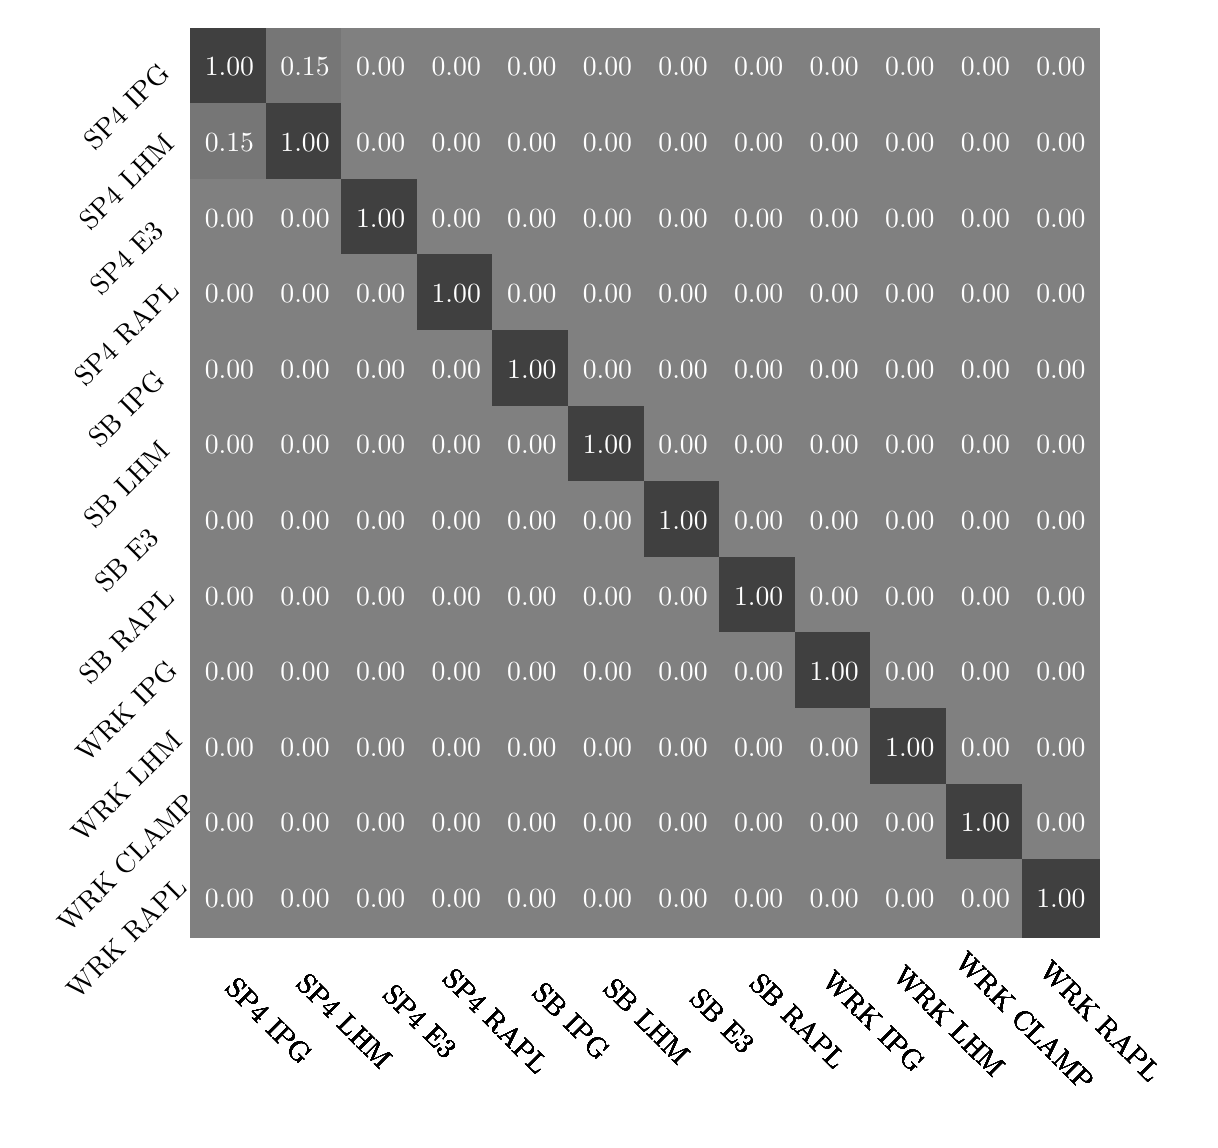
\begin{tikzpicture}[scale=0.6]
    \foreach \y [count=\n] in {{1.00, 0.15, 0.00, 0.00, 0.00, 0.00, 0.00, 0.00, 0.00, 0.00, 0.00, 0.00},{0.15, 1.00, 0.00, 0.00, 0.00, 0.00, 0.00, 0.00, 0.00, 0.00, 0.00, 0.00},{0.00, 0.00, 1.00, 0.00, 0.00, 0.00, 0.00, 0.00, 0.00, 0.00, 0.00, 0.00},{0.00, 0.00, 0.00, 1.00, 0.00, 0.00, 0.00, 0.00, 0.00, 0.00, 0.00, 0.00},{0.00, 0.00, 0.00, 0.00, 1.00, 0.00, 0.00, 0.00, 0.00, 0.00, 0.00, 0.00},{0.00, 0.00, 0.00, 0.00, 0.00, 1.00, 0.00, 0.00, 0.00, 0.00, 0.00, 0.00},{0.00, 0.00, 0.00, 0.00, 0.00, 0.00, 1.00, 0.00, 0.00, 0.00, 0.00, 0.00},{0.00, 0.00, 0.00, 0.00, 0.00, 0.00, 0.00, 1.00, 0.00, 0.00, 0.00, 0.00},{0.00, 0.00, 0.00, 0.00, 0.00, 0.00, 0.00, 0.00, 1.00, 0.00, 0.00, 0.00},{0.00, 0.00, 0.00, 0.00, 0.00, 0.00, 0.00, 0.00, 0.00, 1.00, 0.00, 0.00},{0.00, 0.00, 0.00, 0.00, 0.00, 0.00, 0.00, 0.00, 0.00, 0.00, 1.00, 0.00},{0.00, 0.00, 0.00, 0.00, 0.00, 0.00, 0.00, 0.00, 0.00, 0.00, 0.00, 1.00},} {
    % column labels
    \foreach \a [count=\n] in {SP4 IPG,SP4 LHM,SP4 E3,SP4 RAPL,SB IPG,SB LHM,SB E3,SB RAPL,WRK IPG,WRK LHM,WRK CLAMP,WRK RAPL} {
      \node[minimum size=10mm, xshift=0.5cm, rotate=-45] at (\n*1.6, -21.8) {\a};
    }
    % heatmap tiles
    \foreach \x [count=\m] in \y {
      \pgfmathsetmacro{\xa }{(\x + 1) / 2 * 100}
      \node[fill=darkgray!\xa!lightgray, minimum size=10mm, text=white, font={\normalsize}] at (\m*1.6,-\n*1.6) {\x};
    }
  }
    % row labels
    \foreach \a [count=\i] in {SP4 IPG,SP4 LHM,SP4 E3,SP4 RAPL,SB IPG,SB LHM,SB E3,SB RAPL,WRK IPG,WRK LHM,WRK CLAMP,WRK RAPL} {
      \node[minimum size=10mm, xshift=-0.35cm, yshift=-0.5cm, rotate=45] at (0,-\i*1.6) {\a};
    }
  \end{tikzpicture}
  \caption{Here the results for the FannkuchRedux on the Mann Whitney U Test can be seen. The Range in $0 - 1$}
  \label{tab:HeatFannkuchRedux}
  \end{figure}
\input{tabels/experiment_results/exp_one/StatQuest/Distribution/MannWFasta.tex}
\input{tabels/experiment_results/exp_one/StatQuest/Distribution/MannWNbody.tex}
\input{tabels/experiment_results/exp_one/StatQuest/Distribution/MannWTestCaseIdle.tex}
% \input{tabels/experiment_results/exp_one/StatQuest/Correlation/CompbinedSurfBP.tex}
% \begin{figure}
\centering
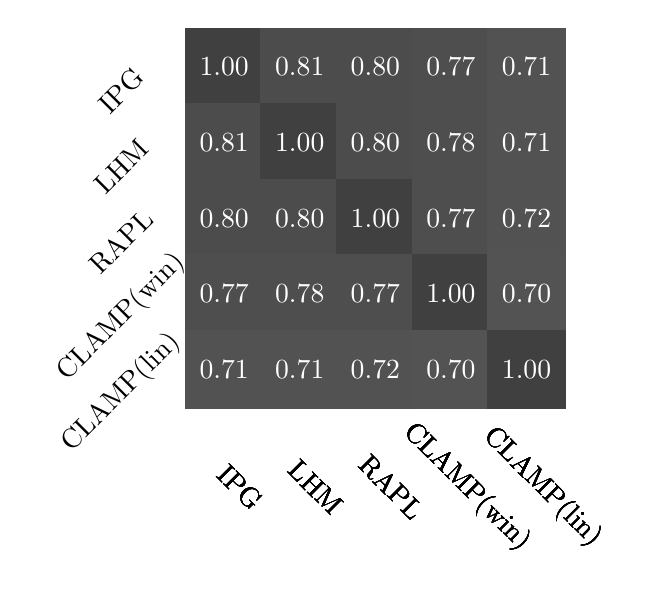
\begin{tikzpicture}[scale=0.6]
  \foreach \y [count=\n] in {{1.00, 0.81, 0.80, 0.77, 0.71},{0.81, 1.00, 0.80, 0.78, 0.71},{0.80, 0.80, 1.00, 0.77, 0.72},{0.77, 0.78, 0.77, 1.00, 0.70},{0.71, 0.71, 0.72, 0.70, 1.00},} {
  % column labels
  \foreach \a [count=\n] in {IPG,LHM,RAPL,CLAMP(win),CLAMP(lin)} {
    \node[minimum size=10mm, xshift=0.2cm, rotate=-45] at (\n*1.6, -10.50) {\a};
  }
  % heatmap tiles
  \foreach \x [count=\m] in \y {
    \pgfmathsetmacro{\xa }{(\x + 1) / 2 * 100}
    \node[fill=darkgray!\xa!lightgray, minimum size=10mm, text=white, font={\normalsize}] at (\m*1.6,-\n*1.6) {\x};
  }
}
  % row labels
  \foreach \a [count=\i] in {IPG,LHM,RAPL,CLAMP(win),CLAMP(lin)} {
    \node[minimum size=10mm, xshift=-0.35cm, yshift=-0.3cm, rotate=45] at (0,-\i*1.6) {\a};
  } 
\end{tikzpicture}
\caption{This heat map represents Correlation coefficients between the different measuring instruments -1 to 1 on the Workstation}
\label{tab:correlationWork}
\end{figure}
\newpage

\section{Statistical results from Experiment \#2}\label{app:stat2}
This results from the statistical analysis of the second experiment, presented in \cref{sec:Stat2}.
% \begin{table}[]
    \begin{tabular}{||c|c|c|c|c|c||}    \hline
    &\textbf{TestCaseIdle}&\textbf{BinaryTrees}&\textbf{FannkuchRedux}&\textbf{Nbody}&\textbf{Fasta}\\ [0.5ex] \hline
    \hline \textbf{IntelPowerGadget}&0.0&0.9103&0.1293&0.0002&0.8291\\
    \textbf{HardwareMonitor}&0.0213&0.1345&0.0492&0.3209&0.0\\
    \textbf{Clamp Win}&0.0034&0.0023&0.012&0.8143&0.5335\\
    \textbf{RAPL}&0.1899&0.5744&0.0015&0.9437&0.0518\\
    \textbf{Clamp Lin}&0.4601&0.0004&0.0&0.1006&0.0002\\ \hline \end{tabular}
    \caption{P values for the normal distribution for the Workstation in Ex2}
    \label{tab:NormDist2}
\end{table}
\input{tabels/experiment_results/exp_two/StatQuest/MannWhitBinary.tex}
% \begin{figure}
    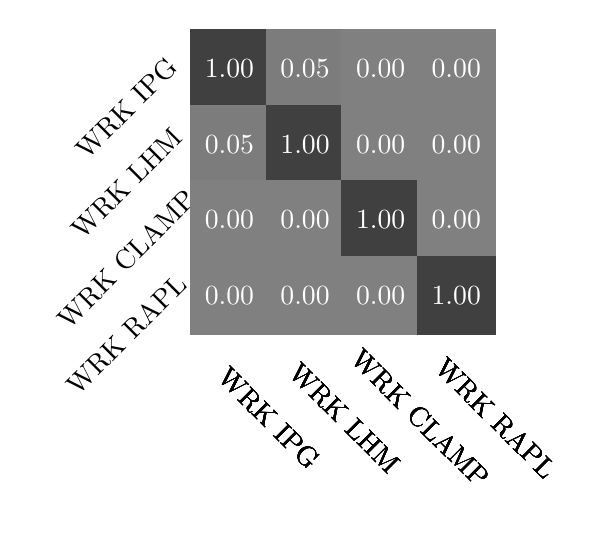
\begin{tikzpicture}[scale=0.6]
      \foreach \y [count=\n] in {{1.00, 0.05, 0.00, 0.00},{0.05, 1.00, 0.00, 0.00},{0.00, 0.00, 1.00, 0.00},{0.00, 0.00, 0.00, 1.00},} {
      % column labels
      \foreach \a [count=\n] in {WRK IPG,WRK LHM,WRK CLAMP,WRK RAPL} {
        \node[minimum size=10mm, xshift=0.5cm, rotate=-45] at (\n*1.6, -9.0) {\a};
      }
      % heatmap tiles
      \foreach \x [count=\m] in \y {
        \pgfmathsetmacro{\xa }{(\x + 1) / 2 * 100}
        \node[fill=darkgray!\xa!lightgray, minimum size=10mm, text=white, font={\normalsize}] at (\m*1.6,-\n*1.6) {\x};
      }
    }
      % row labels
      \foreach \a [count=\i] in {WRK IPG,WRK LHM,WRK CLAMP,WRK RAPL} {
        \node[minimum size=10mm, xshift=-0.35cm, yshift=-0.5cm, rotate=45] at (0,-\i*1.6) {\a};
      }
    \end{tikzpicture}
    \label{tab:HeatFannkuchRedux2}
\end{figure}
\input{tabels/experiment_results/exp_two/StatQuest/MannWhitFasta.tex}
\input{tabels/experiment_results/exp_two/StatQuest/MannwhitIdle.tex}
\input{tabels/experiment_results/exp_two/StatQuest/MannWhitNbody.tex}
% \begin{figure}
    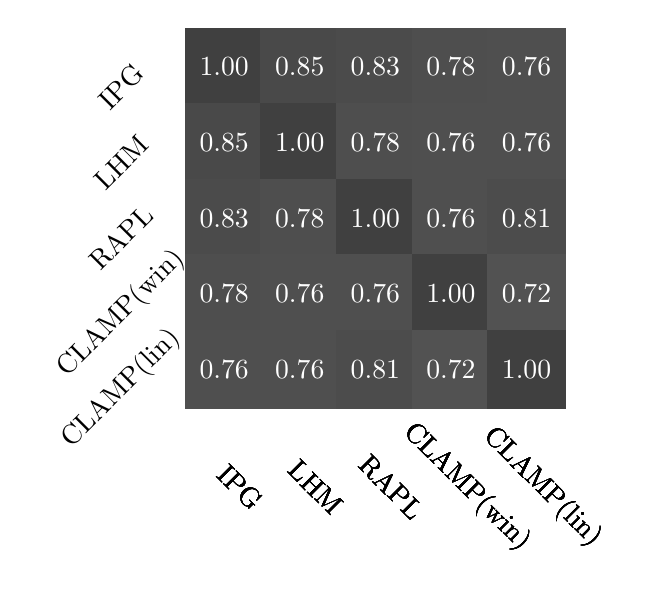
\begin{tikzpicture}[scale=0.6]
      \foreach \y [count=\n] in {{1.00, 0.85, 0.83, 0.78, 0.76},{0.85, 1.00, 0.78, 0.76, 0.76},{0.83, 0.78, 1.00, 0.76, 0.81},{0.78, 0.76, 0.76, 1.00, 0.72},{0.76, 0.76, 0.81, 0.72, 1.00},} {
      % column labels
      \foreach \a [count=\n] in {IPG,LHM,RAPL,CLAMP(win),CLAMP(lin)} {
        \node[minimum size=10mm, xshift=0.2cm, rotate=-45] at (\n*1.6, -10.5) {\a};
      }
      % heatmap tiles
      \foreach \x [count=\m] in \y {
        \pgfmathsetmacro{\xa }{(\x + 1) / 2 * 100}
        \node[fill=darkgray!\xa!lightgray, minimum size=10mm, text=white, font={\normalsize}] at (\m*1.6,-\n*1.6) {\x};
      }
    }
      % row labels
      \foreach \a [count=\i] in {IPG,LHM,RAPL,CLAMP(win),CLAMP(lin)} {
        \node[minimum size=10mm, xshift=-0.35cm, yshift=-0.25cm, rotate=45] at (0,-\i*1.6) {\a};
      }
    \end{tikzpicture}
    \label{tab:correlationWork2}
\end{figure}


















% \begin{figure}
%     \centering
%     \begin{tikzpicture}[]
%         \begin{axis}[ymax=1.6,
%         % axis x line=middle,
%         % axis y line=middle,
%         xlabel={x label},
%         ylabel={y label},
%         ]
%         \addplot[color=blue, mark=square,] coordinates { %% AVG value
%         (0, 1)(0.2, 1)(0.4, 0.8)(0.6, 0.5)(0.8, 0.6)(1, 0.6)
%         };
%         \addplot[color=blue, mark=square,name path=A] coordinates { %% MAX value
%         (0, 1.5)(0.2, 1.1)(0.4, 1.2)(0.6, 1.2)(0.8, 1.3)(1, 1.1)
%         };
%         \addplot[color=blue, mark=square,name path=B] coordinates { %% MIN value
%         (0, 0.9)(0.2, 0.8)(0.4, 0.5)(0.6, 0.4)(0.8, 0.2)(1,0.1)
%         };
%         \addplot [pattern=north east lines,pattern color=red] 
%         fill between [
%             of=A and B,soft clip={domain=-1.5:1.5},
%         ];
%         \end{axis}
% \end{tikzpicture}
% \caption{Graph showing average energy consumption during a run of the experiments} \label{fig:LABEL}
% \end{figure}

% \begin{figure}
%     \centering
%     \begin{tikzpicture}
%         \begin{axis}[
%             xlabel={x label},
%             ylabel={y label},
%         ]
%             \addplot [mark=none, thick, red]  coordinates {
%             (-1.5, 1)(-1, 1)(0, 1)(1, 1)(1.5, 1)
%             };
%             \addlegendentry{eh}
%             \addplot [mark=none, thick, blue] coordinates {
%             (-1.5, 2)(-1, 3)(0, 4)(1, 1)(1.5, -1)
%             };
%             \addlegendentry{oi}
%         \end{axis}
%     \end{tikzpicture} 
% \caption{Graph showing average energy consumption during a run of the experiments} \label{fig:LABEL}
% \end{figure}

% \begin{figure}
%     \centering
%     \begin{tikzpicture}[]
%         \begin{axis}[xlabel={Score}, title={Average performance comparision}, ytick={1,2,3,4},
%         yticklabels={
%             Attentive students,
%             Inattentive students, 
%             Normal students, 
%             Highly participating students
%             },
%             ]
%         \addplot+ [boxplot prepared={
%             lower whisker=25, %%  lower whisker
%             lower quartile=37, %% 25th percentile
%             median=65,  %% a median for the distribution
%             upper quartile=72, %% 75th percentile
%             upper whisker=81}, %%  upper whisker
%             ] table[row sep=\\,y index=0] {1\\ 92\\ 95\\};
%         \addplot+ [boxplot prepared={
%             lower whisker=12, 
%             lower quartile=17, 
%             median=25,
%             upper quartile=52, 
%             upper whisker=61
%             },] table[row sep=\\,y index=0] {\\};
%         \addplot+ [boxplot prepared={
%             lower whisker=12, 
%             lower quartile=25, 
%             median=50,
%             upper quartile=75, 
%             upper whisker=87},] table[row sep=\\,y index=0] {\\};
%         \addplot+ [boxplot prepared={
%             lower whisker=62, 
%             lower quartile=64, 
%             median=70,
%             upper quartile=72, 
%             upper whisker=81
%             },] table[row sep=\\,y index=0] {\\};
%         \end{axis}
%     \end{tikzpicture}
% \caption{Graph comparing performance of different duts and test cases} \label{fig:LABEL01}
% \end{figure}

% \begin{figure}
%     \centering
%     \begin{tikzpicture}[]
%         \begin{axis}[xlabel={XLABEL}, title={TITLE}, ytick={1,2,3,4},
%         yticklabels={
%             Attentive students,
%             },
%             ]
%         \addplot+ [boxplot prepared={
%             lower whisker=25, %%  lower whisker
%             lower quartile=37, %% 25th percentile
%             median=65,  %% a median for the distribution
%             upper quartile=72, %% 75th percentile
%             upper whisker=81}, %%  upper whisker
%             ] table[row sep=\\,y index=0] {1\\ 92\\ 95\\};
%         \end{axis}
%     \end{tikzpicture}
% \caption{CAPTION} \label{fig:LABEL}
% \end{figure}



% \begin{figure}
%     \centering
%     \begin{tikzpicture}[]
%         \begin{axis}[xlabel={xlabel}, title={title}, ytick={1},
%         yticklabels={
%             ytick label
%             },
%             ]
%         \addplot+ [boxplot prepared={
%                 lower whisker=25, %%  lower whisker
%                 lower quartile=37, %% 25th percentile
%                 median=65,  %% a median for the distribution
%                 upper quartile=72, %% 75th percentile
%                 upper whisker=81}, %%  upper whisker
%         ] table[row sep=\\,y index=0] {\\};
%         \end{axis}
%     \end{tikzpicture}
% \caption{caption} \label{fig:label}
% \end{figure}

% 
\begin{figure}
    \centering
    \begin{tikzpicture}
        \begin{axis}[%
        scatter/classes={%
            a={mark=o,draw=black},
            b={mark=o,draw=red}}]
        \addplot[scatter,only marks,%
            scatter src=explicit symbolic]%
        table[meta=label] {
        x y label
        0 2.8949479214654294e-05 a
        1 3.179477203046875e-05 a
        2 3.267322064601172e-05 a
        3 3.280798350852557e-05 a
        4 3.280798350852557e-05 a
        5 4.203733493201637e-05 a
        6 4.2699125166050646e-05 a
        7 4.294905342573423e-05 a
        8 4.676111584622105e-05 a
        9 4.843067177105661e-05 a
        10 4.8774191374681006e-05 a
        11 4.9445616498532656e-05 a
        12 4.9445616498532656e-05 a
        13 4.9958989436862796e-05 a
        14 5.0408826155301995e-05 a
        15 5.0408826155301995e-05 a
        16 5.193014842759746e-05 a
        17 5.634406741910958e-05 a
        18 5.6633789754044637e-05 a
        19 5.6633789754044637e-05 a
        20 5.7410217372431694e-05 a
        21 5.7410217372431694e-05 a
        22 5.921367982846027e-05 a
        23 5.921367982846027e-05 a
        24 6.0456090984576906e-05 a
        25 6.145988034834584e-05 a
        26 6.272460722809678e-05 a
        27 6.284972805645797e-05 a
        28 6.300710443137074e-05 a
        29 6.355470081318446e-05 a
        30 6.359467248323007e-05 a
        31 6.694121683315767e-05 a
        32 6.718318238640716e-05 a
        33 7.127585237345829e-05 a
        34 7.127585237345829e-05 a
        35 7.155322529164951e-05 a
        36 7.38556711976285e-05 a
        37 7.41805540625215e-05 a
        38 7.41805540625215e-05 a
        39 7.765820244366868e-05 a
        40 7.784120665026037e-05 a
        41 7.850775711089268e-05 a
        42 7.993973309373286e-05 a
        43 8.191994222015357e-05 a
        44 8.230819546665794e-05 a
        45 8.420232050680483e-05 a
        46 8.426994000106784e-05 a
        47 8.427717433224613e-05 a
        48 8.479177316626968e-05 a
        49 8.527074308148876e-05 a
        50 8.721724394873936e-05 a
        51 8.722066451929488e-05 a
        52 8.804553811338067e-05 a
        53 8.830233135155855e-05 a
        54 8.975832698738875e-05 a
        55 8.975832698738875e-05 a
        56 8.994826250782899e-05 a
        57 9.030466847320144e-05 a
        58 9.129116493983801e-05 a
        59 9.134194523707361e-05 a
        60 9.161579912448281e-05 a
        61 9.193227245685756e-05 a
        62 9.370516727749144e-05 a
        63 9.370516727749144e-05 a
        64 9.447030026752446e-05 a
        65 9.695684147183935e-05 a
        66 9.84919485426008e-05 a
        67 9.84919485426008e-05 a
        68 9.967369188253414e-05 a
        69 0.00010069773319988507 a
        70 0.00010069773319988507 a
        71 0.00010084232469055083 a
        72 0.00010512257877014406 a
        73 0.00010531121163963648 a
        74 0.00010531121163963648 a
        75 0.00010546120599483379 a
        76 0.00010572136596011746 a
        77 0.00010583143723479704 a
        78 0.00010588947949861364 a
        79 0.00010619424500734341 a
        80 0.00010702116161766447 a
        81 0.00010720818806042881 a
        82 0.00010954500810094572 a
        83 0.00010954500810094572 a
        84 0.00011073430522929063 a
        85 0.00011246416770882411 a
        86 0.0001130661635295037 a
        87 0.00011438558850046904 a
        88 0.00011469125335755415 a
        89 0.00012147392693952117 a
        90 0.00012237591171992 a
        91 0.0001224201334093466 a
        92 0.00012276203358687853 a
        93 0.0001248071419298498 a
        94 0.00012783937274188738 a
        95 0.00012853116577443856 a
        96 0.00013370751331335452 a
        97 0.00013450189840040735 a
        98 0.00013450189840040735 a
        99 0.00013535715902440975 a
        100 0.00013868052735234137 a
        101 0.00013946592819106236 a
        102 0.00013970777345427544 a
        103 0.000146505571066363 a
        104 0.00015101069658064682 a
        105 0.00015706270827900125 a
        106 0.00016013706955956582 a
        107 0.0001662494310569234 a
        108 0.0001669486955830121 a
        109 0.00017282103511564564 a
        110 0.0001741512152900111 a
        111 0.0001867419363296455 a
        112 0.00019374828758415263 a
        113 0.00019483919084249817 a
        114 0.00019699221542950795 a
        115 0.00019850109877225447 a
        116 0.00019912614342020588 a
        117 0.0002031933960156964 a
        118 0.0002232952178907816 a
        119 0.00022506654839991077 a
        120 0.000280816704139863 a
        121 0.0002832259109375601 a
        122 0.00028521681835927984 a
        123 0.00029354421334281766 a
        124 0.0003426297800563272 a
        125 0.00034744633170887413 a
        126 0.0005864789735718681 a
        127 0.0010507104872560743 a
        128 0.012726185306264882 a
        129 0.015124607637026024 a
            };
        \end{axis}
    \end{tikzpicture}
\caption{4-dist sorted graph for } \label{fig:4_dist_sorted_graph}
\end{figure}



% 
                        \begin{figure}
                            \centering
                            \begin{tikzpicture}[]
                                \pgfplotsset{%
                                    width=.7\textwidth,
                                    height=.4\textheight
                                }
                                \begin{axis}[xlabel={Average dynamic energy consumption (Watts)}, title={Dram - Fasta - Dynamic Energy - with outliers}, ytick={1, 2, 3, 4, 5, 6, 7, 8, 9, 10, 11, 12, 13},
                                yticklabels={
                                    SP4 - IPG , SP4 - LHM , SP4 - E3 , SP4 - RAPL , SB - IPG , SB - LHM , SB - E3 , SB - RAPL , WRK - IPG , WRK - LHM , WRK - CLAMP (win) , WRK - RAPL , WRK - CLAMP (lin) 
                                    },
                                    xmin=0,xmax=80,
                                    ]
                                
                                \addplot+ [boxplot prepared={
                                lower whisker=0.10375567387783291,
                                lower quartile=0.11534461113898242,
                                median=0.11826862867259347,
                                upper quartile=0.12268613112552085,
                                upper whisker=0.14669585999344925},
                                ] table[row sep=\\,y index=0] {\\};
                                
                                \addplot+ [boxplot prepared={
                                lower whisker=0.0862842112288128,
                                lower quartile=0.10202879124519204,
                                median=0.10554987794325832,
                                upper quartile=0.10968250635173943,
                                upper whisker=0.1592616793573518},
                                ] table[row sep=\\,y index=0] {\\};
                                
                                \addplot+ [boxplot prepared={
                                lower whisker=0.0,
                                lower quartile=0.0,
                                median=0.0,
                                upper quartile=0.0,
                                upper whisker=0.0},
                                ] table[row sep=\\,y index=0] {\\};
                                
                                \addplot+ [boxplot prepared={
                                lower whisker=-58.376667674084956,
                                lower quartile=24.65499145717873,
                                median=113.55193693398685,
                                upper quartile=201.09246580893398,
                                upper whisker=285.6373247163493},
                                ] table[row sep=\\,y index=0] {\\};
                                
                                \addplot+ [boxplot prepared={
                                lower whisker=0.07774857916188005,
                                lower quartile=0.0873242550944483,
                                median=0.09508604503433815,
                                upper quartile=0.10206423245741358,
                                upper whisker=0.13756539955796498},
                                ] table[row sep=\\,y index=0] {\\};
                                
                                \addplot+ [boxplot prepared={
                                lower whisker=0.07256163691225603,
                                lower quartile=0.08089023223934655,
                                median=0.08963415201613556,
                                upper quartile=0.09406224213444994,
                                upper whisker=0.13676124570877235},
                                ] table[row sep=\\,y index=0] {\\};
                                
                                \addplot+ [boxplot prepared={
                                lower whisker=0.0,
                                lower quartile=0.0,
                                median=0.0,
                                upper quartile=0.0,
                                upper whisker=0.0},
                                ] table[row sep=\\,y index=0] {\\};
                                
                                \addplot+ [boxplot prepared={
                                lower whisker=-37.044547337624394,
                                lower quartile=-1.4124469487498352,
                                median=35.64065726225357,
                                upper quartile=72.48940753615494,
                                upper whisker=113.22179616624354},
                                ] table[row sep=\\,y index=0] {\\};
                                
                                \addplot+ [boxplot prepared={
                                lower whisker=0.013368045961463015,
                                lower quartile=0.016088896176256334,
                                median=0.01687580237366476,
                                upper quartile=0.017975615001784323,
                                upper whisker=0.10726491114142167},
                                ] table[row sep=\\,y index=0] {\\};
                                
                                \addplot+ [boxplot prepared={
                                lower whisker=0.013483540437493668,
                                lower quartile=0.016545480037850613,
                                median=0.016984038349566133,
                                upper quartile=0.01806521189896282,
                                upper whisker=0.10485184969555783},
                                ] table[row sep=\\,y index=0] {\\};
                                
                                \addplot+ [boxplot prepared={
                                lower whisker=0.0,
                                lower quartile=0.0,
                                median=0.0,
                                upper quartile=0.0,
                                upper whisker=0.0},
                                ] table[row sep=\\,y index=0] {\\};
                                
                                \addplot+ [boxplot prepared={
                                lower whisker=-4.312948877137323,
                                lower quartile=563.2009907152465,
                                median=1130.2995209910928,
                                upper quartile=1699.72830809869,
                                upper whisker=2265.3777432909205},
                                ] table[row sep=\\,y index=0] {\\};
                                
                                \addplot+ [boxplot prepared={
                                lower whisker=0.0,
                                lower quartile=0.0,
                                median=0.0,
                                upper quartile=0.0,
                                upper whisker=0.0},
                                ] table[row sep=\\,y index=0] {\\};
                                
                                \end{axis}
                            \end{tikzpicture}
                        \caption{A comparison of of Dram dynamic energy consumption for test case Fasta for all DUT's and OS's  (with outliers)} \label{fig:Fasta_Dram_comparison_dynamic_energy_with_outliers_avg_watts}
                        \end{figure}
                        
% 
                        \begin{figure}
                            \centering
                            \begin{tikzpicture}[]
                                \pgfplotsset{%
                                    width=.7\textwidth,
                                    height=.4\textheight
                                }
                                \begin{axis}[xlabel={Average dynamic energy consumption (Watts)}, title={Dram - Fasta - Dynamic Energy - with outliers}, ytick={1, 2, 3, 4, 5, 6, 7, 8, 9, 10, 11, 12, 13},
                                yticklabels={
                                    SP4 - IPG , SP4 - LHM , SP4 - E3 , SP4 - RAPL , SB - IPG , SB - LHM , SB - E3 , SB - RAPL , WRK - IPG , WRK - LHM , WRK - CLAMP (win) , WRK - RAPL , WRK - CLAMP (lin) 
                                    },
                                    xmin=0,xmax=80,
                                    ]
                                
                                \addplot+ [boxplot prepared={
                                lower whisker=0.10375567387783291,
                                lower quartile=0.11534461113898242,
                                median=0.11826862867259347,
                                upper quartile=0.12268613112552085,
                                upper whisker=0.14669585999344925},
                                ] table[row sep=\\,y index=0] {\\};
                                
                                \addplot+ [boxplot prepared={
                                lower whisker=0.0862842112288128,
                                lower quartile=0.10202879124519204,
                                median=0.10554987794325832,
                                upper quartile=0.10968250635173943,
                                upper whisker=0.1592616793573518},
                                ] table[row sep=\\,y index=0] {\\};
                                
                                \addplot+ [boxplot prepared={
                                lower whisker=0.0,
                                lower quartile=0.0,
                                median=0.0,
                                upper quartile=0.0,
                                upper whisker=0.0},
                                ] table[row sep=\\,y index=0] {\\};
                                
                                \addplot+ [boxplot prepared={
                                lower whisker=-58.376667674084956,
                                lower quartile=24.65499145717873,
                                median=113.55193693398685,
                                upper quartile=201.09246580893398,
                                upper whisker=285.6373247163493},
                                ] table[row sep=\\,y index=0] {\\};
                                
                                \addplot+ [boxplot prepared={
                                lower whisker=0.07774857916188005,
                                lower quartile=0.0873242550944483,
                                median=0.09508604503433815,
                                upper quartile=0.10206423245741358,
                                upper whisker=0.13756539955796498},
                                ] table[row sep=\\,y index=0] {\\};
                                
                                \addplot+ [boxplot prepared={
                                lower whisker=0.07256163691225603,
                                lower quartile=0.08089023223934655,
                                median=0.08963415201613556,
                                upper quartile=0.09406224213444994,
                                upper whisker=0.13676124570877235},
                                ] table[row sep=\\,y index=0] {\\};
                                
                                \addplot+ [boxplot prepared={
                                lower whisker=0.0,
                                lower quartile=0.0,
                                median=0.0,
                                upper quartile=0.0,
                                upper whisker=0.0},
                                ] table[row sep=\\,y index=0] {\\};
                                
                                \addplot+ [boxplot prepared={
                                lower whisker=-37.044547337624394,
                                lower quartile=-1.4124469487498352,
                                median=35.64065726225357,
                                upper quartile=72.48940753615494,
                                upper whisker=113.22179616624354},
                                ] table[row sep=\\,y index=0] {\\};
                                
                                \addplot+ [boxplot prepared={
                                lower whisker=0.013368045961463015,
                                lower quartile=0.016088896176256334,
                                median=0.01687580237366476,
                                upper quartile=0.017975615001784323,
                                upper whisker=0.10726491114142167},
                                ] table[row sep=\\,y index=0] {\\};
                                
                                \addplot+ [boxplot prepared={
                                lower whisker=0.013483540437493668,
                                lower quartile=0.016545480037850613,
                                median=0.016984038349566133,
                                upper quartile=0.01806521189896282,
                                upper whisker=0.10485184969555783},
                                ] table[row sep=\\,y index=0] {\\};
                                
                                \addplot+ [boxplot prepared={
                                lower whisker=0.0,
                                lower quartile=0.0,
                                median=0.0,
                                upper quartile=0.0,
                                upper whisker=0.0},
                                ] table[row sep=\\,y index=0] {\\};
                                
                                \addplot+ [boxplot prepared={
                                lower whisker=-4.312948877137323,
                                lower quartile=563.2009907152465,
                                median=1130.2995209910928,
                                upper quartile=1699.72830809869,
                                upper whisker=2265.3777432909205},
                                ] table[row sep=\\,y index=0] {\\};
                                
                                \addplot+ [boxplot prepared={
                                lower whisker=0.0,
                                lower quartile=0.0,
                                median=0.0,
                                upper quartile=0.0,
                                upper whisker=0.0},
                                ] table[row sep=\\,y index=0] {\\};
                                
                                \end{axis}
                            \end{tikzpicture}
                        \caption{A comparison of of Dram dynamic energy consumption for test case Fasta for all DUT's and OS's  (with outliers)} \label{fig:Fasta_Dram_comparison_dynamic_energy_with_outliers_avg_watts}
                        \end{figure}
                        
% 
                        \begin{figure}
                            \centering
                            \begin{tikzpicture}[]
                                \pgfplotsset{%
                                    width=.7\textwidth,
                                    height=.4\textheight
                                }
                                \begin{axis}[xlabel={Average dynamic energy consumption (Watts)}, title={Dram - Fasta - Dynamic Energy - with outliers}, ytick={1, 2, 3, 4, 5, 6, 7, 8, 9, 10, 11, 12, 13},
                                yticklabels={
                                    SP4 - IPG , SP4 - LHM , SP4 - E3 , SP4 - RAPL , SB - IPG , SB - LHM , SB - E3 , SB - RAPL , WRK - IPG , WRK - LHM , WRK - CLAMP (win) , WRK - RAPL , WRK - CLAMP (lin) 
                                    },
                                    xmin=0,xmax=80,
                                    ]
                                
                                \addplot+ [boxplot prepared={
                                lower whisker=0.10375567387783291,
                                lower quartile=0.11534461113898242,
                                median=0.11826862867259347,
                                upper quartile=0.12268613112552085,
                                upper whisker=0.14669585999344925},
                                ] table[row sep=\\,y index=0] {\\};
                                
                                \addplot+ [boxplot prepared={
                                lower whisker=0.0862842112288128,
                                lower quartile=0.10202879124519204,
                                median=0.10554987794325832,
                                upper quartile=0.10968250635173943,
                                upper whisker=0.1592616793573518},
                                ] table[row sep=\\,y index=0] {\\};
                                
                                \addplot+ [boxplot prepared={
                                lower whisker=0.0,
                                lower quartile=0.0,
                                median=0.0,
                                upper quartile=0.0,
                                upper whisker=0.0},
                                ] table[row sep=\\,y index=0] {\\};
                                
                                \addplot+ [boxplot prepared={
                                lower whisker=-58.376667674084956,
                                lower quartile=24.65499145717873,
                                median=113.55193693398685,
                                upper quartile=201.09246580893398,
                                upper whisker=285.6373247163493},
                                ] table[row sep=\\,y index=0] {\\};
                                
                                \addplot+ [boxplot prepared={
                                lower whisker=0.07774857916188005,
                                lower quartile=0.0873242550944483,
                                median=0.09508604503433815,
                                upper quartile=0.10206423245741358,
                                upper whisker=0.13756539955796498},
                                ] table[row sep=\\,y index=0] {\\};
                                
                                \addplot+ [boxplot prepared={
                                lower whisker=0.07256163691225603,
                                lower quartile=0.08089023223934655,
                                median=0.08963415201613556,
                                upper quartile=0.09406224213444994,
                                upper whisker=0.13676124570877235},
                                ] table[row sep=\\,y index=0] {\\};
                                
                                \addplot+ [boxplot prepared={
                                lower whisker=0.0,
                                lower quartile=0.0,
                                median=0.0,
                                upper quartile=0.0,
                                upper whisker=0.0},
                                ] table[row sep=\\,y index=0] {\\};
                                
                                \addplot+ [boxplot prepared={
                                lower whisker=-37.044547337624394,
                                lower quartile=-1.4124469487498352,
                                median=35.64065726225357,
                                upper quartile=72.48940753615494,
                                upper whisker=113.22179616624354},
                                ] table[row sep=\\,y index=0] {\\};
                                
                                \addplot+ [boxplot prepared={
                                lower whisker=0.013368045961463015,
                                lower quartile=0.016088896176256334,
                                median=0.01687580237366476,
                                upper quartile=0.017975615001784323,
                                upper whisker=0.10726491114142167},
                                ] table[row sep=\\,y index=0] {\\};
                                
                                \addplot+ [boxplot prepared={
                                lower whisker=0.013483540437493668,
                                lower quartile=0.016545480037850613,
                                median=0.016984038349566133,
                                upper quartile=0.01806521189896282,
                                upper whisker=0.10485184969555783},
                                ] table[row sep=\\,y index=0] {\\};
                                
                                \addplot+ [boxplot prepared={
                                lower whisker=0.0,
                                lower quartile=0.0,
                                median=0.0,
                                upper quartile=0.0,
                                upper whisker=0.0},
                                ] table[row sep=\\,y index=0] {\\};
                                
                                \addplot+ [boxplot prepared={
                                lower whisker=-4.312948877137323,
                                lower quartile=563.2009907152465,
                                median=1130.2995209910928,
                                upper quartile=1699.72830809869,
                                upper whisker=2265.3777432909205},
                                ] table[row sep=\\,y index=0] {\\};
                                
                                \addplot+ [boxplot prepared={
                                lower whisker=0.0,
                                lower quartile=0.0,
                                median=0.0,
                                upper quartile=0.0,
                                upper whisker=0.0},
                                ] table[row sep=\\,y index=0] {\\};
                                
                                \end{axis}
                            \end{tikzpicture}
                        \caption{A comparison of of Dram dynamic energy consumption for test case Fasta for all DUT's and OS's  (with outliers)} \label{fig:Fasta_Dram_comparison_dynamic_energy_with_outliers_avg_watts}
                        \end{figure}
                        
% 
                        \begin{figure}
                            \centering
                            \begin{tikzpicture}[]
                                \pgfplotsset{%
                                    width=.7\textwidth,
                                    height=.4\textheight
                                }
                                \begin{axis}[xlabel={Average dynamic energy consumption (Watts)}, title={Dram - Fasta - Dynamic Energy - with outliers}, ytick={1, 2, 3, 4, 5, 6, 7, 8, 9, 10, 11, 12, 13},
                                yticklabels={
                                    SP4 - IPG , SP4 - LHM , SP4 - E3 , SP4 - RAPL , SB - IPG , SB - LHM , SB - E3 , SB - RAPL , WRK - IPG , WRK - LHM , WRK - CLAMP (win) , WRK - RAPL , WRK - CLAMP (lin) 
                                    },
                                    xmin=0,xmax=80,
                                    ]
                                
                                \addplot+ [boxplot prepared={
                                lower whisker=0.10375567387783291,
                                lower quartile=0.11534461113898242,
                                median=0.11826862867259347,
                                upper quartile=0.12268613112552085,
                                upper whisker=0.14669585999344925},
                                ] table[row sep=\\,y index=0] {\\};
                                
                                \addplot+ [boxplot prepared={
                                lower whisker=0.0862842112288128,
                                lower quartile=0.10202879124519204,
                                median=0.10554987794325832,
                                upper quartile=0.10968250635173943,
                                upper whisker=0.1592616793573518},
                                ] table[row sep=\\,y index=0] {\\};
                                
                                \addplot+ [boxplot prepared={
                                lower whisker=0.0,
                                lower quartile=0.0,
                                median=0.0,
                                upper quartile=0.0,
                                upper whisker=0.0},
                                ] table[row sep=\\,y index=0] {\\};
                                
                                \addplot+ [boxplot prepared={
                                lower whisker=-58.376667674084956,
                                lower quartile=24.65499145717873,
                                median=113.55193693398685,
                                upper quartile=201.09246580893398,
                                upper whisker=285.6373247163493},
                                ] table[row sep=\\,y index=0] {\\};
                                
                                \addplot+ [boxplot prepared={
                                lower whisker=0.07774857916188005,
                                lower quartile=0.0873242550944483,
                                median=0.09508604503433815,
                                upper quartile=0.10206423245741358,
                                upper whisker=0.13756539955796498},
                                ] table[row sep=\\,y index=0] {\\};
                                
                                \addplot+ [boxplot prepared={
                                lower whisker=0.07256163691225603,
                                lower quartile=0.08089023223934655,
                                median=0.08963415201613556,
                                upper quartile=0.09406224213444994,
                                upper whisker=0.13676124570877235},
                                ] table[row sep=\\,y index=0] {\\};
                                
                                \addplot+ [boxplot prepared={
                                lower whisker=0.0,
                                lower quartile=0.0,
                                median=0.0,
                                upper quartile=0.0,
                                upper whisker=0.0},
                                ] table[row sep=\\,y index=0] {\\};
                                
                                \addplot+ [boxplot prepared={
                                lower whisker=-37.044547337624394,
                                lower quartile=-1.4124469487498352,
                                median=35.64065726225357,
                                upper quartile=72.48940753615494,
                                upper whisker=113.22179616624354},
                                ] table[row sep=\\,y index=0] {\\};
                                
                                \addplot+ [boxplot prepared={
                                lower whisker=0.013368045961463015,
                                lower quartile=0.016088896176256334,
                                median=0.01687580237366476,
                                upper quartile=0.017975615001784323,
                                upper whisker=0.10726491114142167},
                                ] table[row sep=\\,y index=0] {\\};
                                
                                \addplot+ [boxplot prepared={
                                lower whisker=0.013483540437493668,
                                lower quartile=0.016545480037850613,
                                median=0.016984038349566133,
                                upper quartile=0.01806521189896282,
                                upper whisker=0.10485184969555783},
                                ] table[row sep=\\,y index=0] {\\};
                                
                                \addplot+ [boxplot prepared={
                                lower whisker=0.0,
                                lower quartile=0.0,
                                median=0.0,
                                upper quartile=0.0,
                                upper whisker=0.0},
                                ] table[row sep=\\,y index=0] {\\};
                                
                                \addplot+ [boxplot prepared={
                                lower whisker=-4.312948877137323,
                                lower quartile=563.2009907152465,
                                median=1130.2995209910928,
                                upper quartile=1699.72830809869,
                                upper whisker=2265.3777432909205},
                                ] table[row sep=\\,y index=0] {\\};
                                
                                \addplot+ [boxplot prepared={
                                lower whisker=0.0,
                                lower quartile=0.0,
                                median=0.0,
                                upper quartile=0.0,
                                upper whisker=0.0},
                                ] table[row sep=\\,y index=0] {\\};
                                
                                \end{axis}
                            \end{tikzpicture}
                        \caption{A comparison of of Dram dynamic energy consumption for test case Fasta for all DUT's and OS's  (with outliers)} \label{fig:Fasta_Dram_comparison_dynamic_energy_with_outliers_avg_watts}
                        \end{figure}
                        
% 
                        \begin{figure}
                            \centering
                            \begin{tikzpicture}[]
                                \pgfplotsset{%
                                    width=.7\textwidth,
                                    height=.4\textheight
                                }
                                \begin{axis}[xlabel={Average dynamic energy consumption (Watts)}, title={Dram - Fasta - Dynamic Energy - with outliers}, ytick={1, 2, 3, 4, 5, 6, 7, 8, 9, 10, 11, 12, 13},
                                yticklabels={
                                    SP4 - IPG , SP4 - LHM , SP4 - E3 , SP4 - RAPL , SB - IPG , SB - LHM , SB - E3 , SB - RAPL , WRK - IPG , WRK - LHM , WRK - CLAMP (win) , WRK - RAPL , WRK - CLAMP (lin) 
                                    },
                                    xmin=0,xmax=80,
                                    ]
                                
                                \addplot+ [boxplot prepared={
                                lower whisker=0.10375567387783291,
                                lower quartile=0.11534461113898242,
                                median=0.11826862867259347,
                                upper quartile=0.12268613112552085,
                                upper whisker=0.14669585999344925},
                                ] table[row sep=\\,y index=0] {\\};
                                
                                \addplot+ [boxplot prepared={
                                lower whisker=0.0862842112288128,
                                lower quartile=0.10202879124519204,
                                median=0.10554987794325832,
                                upper quartile=0.10968250635173943,
                                upper whisker=0.1592616793573518},
                                ] table[row sep=\\,y index=0] {\\};
                                
                                \addplot+ [boxplot prepared={
                                lower whisker=0.0,
                                lower quartile=0.0,
                                median=0.0,
                                upper quartile=0.0,
                                upper whisker=0.0},
                                ] table[row sep=\\,y index=0] {\\};
                                
                                \addplot+ [boxplot prepared={
                                lower whisker=-58.376667674084956,
                                lower quartile=24.65499145717873,
                                median=113.55193693398685,
                                upper quartile=201.09246580893398,
                                upper whisker=285.6373247163493},
                                ] table[row sep=\\,y index=0] {\\};
                                
                                \addplot+ [boxplot prepared={
                                lower whisker=0.07774857916188005,
                                lower quartile=0.0873242550944483,
                                median=0.09508604503433815,
                                upper quartile=0.10206423245741358,
                                upper whisker=0.13756539955796498},
                                ] table[row sep=\\,y index=0] {\\};
                                
                                \addplot+ [boxplot prepared={
                                lower whisker=0.07256163691225603,
                                lower quartile=0.08089023223934655,
                                median=0.08963415201613556,
                                upper quartile=0.09406224213444994,
                                upper whisker=0.13676124570877235},
                                ] table[row sep=\\,y index=0] {\\};
                                
                                \addplot+ [boxplot prepared={
                                lower whisker=0.0,
                                lower quartile=0.0,
                                median=0.0,
                                upper quartile=0.0,
                                upper whisker=0.0},
                                ] table[row sep=\\,y index=0] {\\};
                                
                                \addplot+ [boxplot prepared={
                                lower whisker=-37.044547337624394,
                                lower quartile=-1.4124469487498352,
                                median=35.64065726225357,
                                upper quartile=72.48940753615494,
                                upper whisker=113.22179616624354},
                                ] table[row sep=\\,y index=0] {\\};
                                
                                \addplot+ [boxplot prepared={
                                lower whisker=0.013368045961463015,
                                lower quartile=0.016088896176256334,
                                median=0.01687580237366476,
                                upper quartile=0.017975615001784323,
                                upper whisker=0.10726491114142167},
                                ] table[row sep=\\,y index=0] {\\};
                                
                                \addplot+ [boxplot prepared={
                                lower whisker=0.013483540437493668,
                                lower quartile=0.016545480037850613,
                                median=0.016984038349566133,
                                upper quartile=0.01806521189896282,
                                upper whisker=0.10485184969555783},
                                ] table[row sep=\\,y index=0] {\\};
                                
                                \addplot+ [boxplot prepared={
                                lower whisker=0.0,
                                lower quartile=0.0,
                                median=0.0,
                                upper quartile=0.0,
                                upper whisker=0.0},
                                ] table[row sep=\\,y index=0] {\\};
                                
                                \addplot+ [boxplot prepared={
                                lower whisker=-4.312948877137323,
                                lower quartile=563.2009907152465,
                                median=1130.2995209910928,
                                upper quartile=1699.72830809869,
                                upper whisker=2265.3777432909205},
                                ] table[row sep=\\,y index=0] {\\};
                                
                                \addplot+ [boxplot prepared={
                                lower whisker=0.0,
                                lower quartile=0.0,
                                median=0.0,
                                upper quartile=0.0,
                                upper whisker=0.0},
                                ] table[row sep=\\,y index=0] {\\};
                                
                                \end{axis}
                            \end{tikzpicture}
                        \caption{A comparison of of Dram dynamic energy consumption for test case Fasta for all DUT's and OS's  (with outliers)} \label{fig:Fasta_Dram_comparison_dynamic_energy_with_outliers_avg_watts}
                        \end{figure}
                        

% 
                        \begin{figure}
                            \centering
                            \begin{tikzpicture}[]
                                \pgfplotsset{%
                                    width=.85\textwidth,
                                    height=.4\textheight
                                }
                                \begin{axis}[xlabel={Average dynamic energy consumption (Watts)}, title={Cores - BinaryTrees - Dynamic Energy - with outliers}, ytick={1, 2, 3, 4, 5, 6, 7, 8, 9, 10, 11, 12, 13},
                                yticklabels={
                                    SP4 - IPG , SP4 - LHM , SP4 - E3 , SP4 - RAPL , SB - IPG , SB - LHM , SB - E3 , SB - RAPL , WRK - IPG , WRK - LHM , WRK - CLAMP (win) , WRK - RAPL , WRK - CLAMP (lin) 
                                    },
                                    xmin=0,xmax=80,
                                    ]
                                
                                \addplot+ [boxplot prepared={
                                lower whisker=11.420748362866629,
                                lower quartile=12.6580266708996,
                                median=13.130573674940711,
                                upper quartile=13.607831789003136,
                                upper whisker=14.46411097772971},
                                ] table[row sep=\\,y index=0] {\\};
                                
                                \addplot+ [boxplot prepared={
                                lower whisker=11.376920355725565,
                                lower quartile=11.859438510771918,
                                median=12.021494244664462,
                                upper quartile=12.198808082967586,
                                upper whisker=12.733883887273084},
                                ] table[row sep=\\,y index=0] {\\};
                                
                                \addplot+ [boxplot prepared={
                                lower whisker=11.219893282713638,
                                lower quartile=11.392272070684548,
                                median=11.517371341746154,
                                upper quartile=11.621194830198572,
                                upper whisker=11.904963494099112},
                                ] table[row sep=\\,y index=0] {\\};
                                
                                \addplot+ [boxplot prepared={
                                lower whisker=7.858040649665969,
                                lower quartile=8.009985603972664,
                                median=8.035629334355505,
                                upper quartile=8.056069699901885,
                                upper whisker=8.115869058828618},
                                ] table[row sep=\\,y index=0] {\\};
                                
                                \addplot+ [boxplot prepared={
                                lower whisker=2.262212420881607,
                                lower quartile=2.665594787259187,
                                median=3.0824671350351713,
                                upper quartile=4.358960214695252,
                                upper whisker=6.1735648226258775},
                                ] table[row sep=\\,y index=0] {\\};
                                
                                \addplot+ [boxplot prepared={
                                lower whisker=1.3655759382792674,
                                lower quartile=2.523121921079479,
                                median=3.3460963285486782,
                                upper quartile=4.425424940316596,
                                upper whisker=6.272376418833985},
                                ] table[row sep=\\,y index=0] {\\};
                                
                                \addplot+ [boxplot prepared={
                                lower whisker=2.3566196168660305,
                                lower quartile=3.3153296051298047,
                                median=4.085362353031364,
                                upper quartile=4.835337745266552,
                                upper whisker=6.151594431657646},
                                ] table[row sep=\\,y index=0] {\\};
                                
                                \addplot+ [boxplot prepared={
                                lower whisker=4.828483342208097,
                                lower quartile=4.964034824723491,
                                median=5.116431256812656,
                                upper quartile=5.289743479362281,
                                upper whisker=5.625244550954983},
                                ] table[row sep=\\,y index=0] {\\};
                                
                                \addplot+ [boxplot prepared={
                                lower whisker=66.89792094118035,
                                lower quartile=67.82648820588565,
                                median=68.22365397596283,
                                upper quartile=68.53649902422302,
                                upper whisker=72.91899239828562},
                                ] table[row sep=\\,y index=0] {\\};
                                
                                \addplot+ [boxplot prepared={
                                lower whisker=65.4708069509544,
                                lower quartile=66.11534816821023,
                                median=66.27532723833454,
                                upper quartile=66.44412633159524,
                                upper whisker=69.64149630164013},
                                ] table[row sep=\\,y index=0] {\\};
                                
                                \addplot+ [boxplot prepared={
                                lower whisker=49.36748648899456,
                                lower quartile=59.39957521748035,
                                median=60.22154751822312,
                                upper quartile=68.57561563020016,
                                upper whisker=76.59487529684452},
                                ] table[row sep=\\,y index=0] {\\};
                                
                                \addplot+ [boxplot prepared={
                                lower whisker=56.400276110515385,
                                lower quartile=56.75939325693689,
                                median=56.86448126331913,
                                upper quartile=56.965123398456655,
                                upper whisker=57.15490760460869},
                                ] table[row sep=\\,y index=0] {\\};
                                
                                \addplot+ [boxplot prepared={
                                lower whisker=34.2500767117359,
                                lower quartile=51.50619275990899,
                                median=52.32916789904128,
                                upper quartile=52.74930164067668,
                                upper whisker=72.15287309502655},
                                ] table[row sep=\\,y index=0] {\\};
                                
                                \end{axis}
                            \end{tikzpicture}
                        \caption{A comparison of Cores dynamic energy consumption for test case BinaryTrees for all DUT's and OS's  (with outliers)} \label{fig:BinaryTrees_Cores_comparison_dynamic_energy_with_outliers_avg_watts}
                        \end{figure}
                        
% 
                        \begin{figure}
                            \centering
                            \begin{tikzpicture}[]
                                \pgfplotsset{%
                                    width=.7\textwidth,
                                    height=.4\textheight
                                }
                                \begin{axis}[xlabel={Average dynamic energy consumption (Watts)}, title={Dram - Fasta - Dynamic Energy - with outliers}, ytick={1, 2, 3, 4, 5, 6, 7, 8, 9, 10, 11, 12, 13},
                                yticklabels={
                                    SP4 - IPG , SP4 - LHM , SP4 - E3 , SP4 - RAPL , SB - IPG , SB - LHM , SB - E3 , SB - RAPL , WRK - IPG , WRK - LHM , WRK - CLAMP (win) , WRK - RAPL , WRK - CLAMP (lin) 
                                    },
                                    xmin=0,xmax=80,
                                    ]
                                
                                \addplot+ [boxplot prepared={
                                lower whisker=0.10375567387783291,
                                lower quartile=0.11534461113898242,
                                median=0.11826862867259347,
                                upper quartile=0.12268613112552085,
                                upper whisker=0.14669585999344925},
                                ] table[row sep=\\,y index=0] {\\};
                                
                                \addplot+ [boxplot prepared={
                                lower whisker=0.0862842112288128,
                                lower quartile=0.10202879124519204,
                                median=0.10554987794325832,
                                upper quartile=0.10968250635173943,
                                upper whisker=0.1592616793573518},
                                ] table[row sep=\\,y index=0] {\\};
                                
                                \addplot+ [boxplot prepared={
                                lower whisker=0.0,
                                lower quartile=0.0,
                                median=0.0,
                                upper quartile=0.0,
                                upper whisker=0.0},
                                ] table[row sep=\\,y index=0] {\\};
                                
                                \addplot+ [boxplot prepared={
                                lower whisker=-58.376667674084956,
                                lower quartile=24.65499145717873,
                                median=113.55193693398685,
                                upper quartile=201.09246580893398,
                                upper whisker=285.6373247163493},
                                ] table[row sep=\\,y index=0] {\\};
                                
                                \addplot+ [boxplot prepared={
                                lower whisker=0.07774857916188005,
                                lower quartile=0.0873242550944483,
                                median=0.09508604503433815,
                                upper quartile=0.10206423245741358,
                                upper whisker=0.13756539955796498},
                                ] table[row sep=\\,y index=0] {\\};
                                
                                \addplot+ [boxplot prepared={
                                lower whisker=0.07256163691225603,
                                lower quartile=0.08089023223934655,
                                median=0.08963415201613556,
                                upper quartile=0.09406224213444994,
                                upper whisker=0.13676124570877235},
                                ] table[row sep=\\,y index=0] {\\};
                                
                                \addplot+ [boxplot prepared={
                                lower whisker=0.0,
                                lower quartile=0.0,
                                median=0.0,
                                upper quartile=0.0,
                                upper whisker=0.0},
                                ] table[row sep=\\,y index=0] {\\};
                                
                                \addplot+ [boxplot prepared={
                                lower whisker=-37.044547337624394,
                                lower quartile=-1.4124469487498352,
                                median=35.64065726225357,
                                upper quartile=72.48940753615494,
                                upper whisker=113.22179616624354},
                                ] table[row sep=\\,y index=0] {\\};
                                
                                \addplot+ [boxplot prepared={
                                lower whisker=0.013368045961463015,
                                lower quartile=0.016088896176256334,
                                median=0.01687580237366476,
                                upper quartile=0.017975615001784323,
                                upper whisker=0.10726491114142167},
                                ] table[row sep=\\,y index=0] {\\};
                                
                                \addplot+ [boxplot prepared={
                                lower whisker=0.013483540437493668,
                                lower quartile=0.016545480037850613,
                                median=0.016984038349566133,
                                upper quartile=0.01806521189896282,
                                upper whisker=0.10485184969555783},
                                ] table[row sep=\\,y index=0] {\\};
                                
                                \addplot+ [boxplot prepared={
                                lower whisker=0.0,
                                lower quartile=0.0,
                                median=0.0,
                                upper quartile=0.0,
                                upper whisker=0.0},
                                ] table[row sep=\\,y index=0] {\\};
                                
                                \addplot+ [boxplot prepared={
                                lower whisker=-4.312948877137323,
                                lower quartile=563.2009907152465,
                                median=1130.2995209910928,
                                upper quartile=1699.72830809869,
                                upper whisker=2265.3777432909205},
                                ] table[row sep=\\,y index=0] {\\};
                                
                                \addplot+ [boxplot prepared={
                                lower whisker=0.0,
                                lower quartile=0.0,
                                median=0.0,
                                upper quartile=0.0,
                                upper whisker=0.0},
                                ] table[row sep=\\,y index=0] {\\};
                                
                                \end{axis}
                            \end{tikzpicture}
                        \caption{A comparison of of Dram dynamic energy consumption for test case Fasta for all DUT's and OS's  (with outliers)} \label{fig:Fasta_Dram_comparison_dynamic_energy_with_outliers_avg_watts}
                        \end{figure}
                        
% 
                            \begin{figure}
                                \centering
                                \begin{tikzpicture}[]
                                    \pgfplotsset{%
                                        width=.85\textwidth,
                                        height=.15\textheight
                                    }
                                    \begin{axis}[xlabel={Average energy consumption (Watts)}, title={Cores - Nbody - Energy - with outliers}, ytick={1, 2, 3, 4},
                                    yticklabels={
                                        IPG , LHM , E3 , RAPL 
                                        },
                                        xmin=0,xmax=10,
                                        ]
                                    
                                    \addplot+ [boxplot prepared={
                                    lower whisker=3.3904966623857957,
                                    lower quartile=3.590049859121917,
                                    median=3.659495158384077,
                                    upper quartile=3.7265303388398676,
                                    upper whisker=3.961455824832631},
                                    ] table[row sep=\\,y index=0] {\\};
                                    
                                    \addplot+ [boxplot prepared={
                                    lower whisker=4.310300897881025,
                                    lower quartile=4.399235063852297,
                                    median=4.436051030948529,
                                    upper quartile=4.4760085282539865,
                                    upper whisker=4.578699108862436},
                                    ] table[row sep=\\,y index=0] {\\};
                                    
                                    \addplot+ [boxplot prepared={
                                    lower whisker=2.399996038382789,
                                    lower quartile=4.241702359737292,
                                    median=4.27199328109721,
                                    upper quartile=4.302908157167919,
                                    upper whisker=4.369796102164826},
                                    ] table[row sep=\\,y index=0] {\\};
                                    
                                    \addplot+ [boxplot prepared={
                                    lower whisker=8.442268947178363,
                                    lower quartile=8.469458770450048,
                                    median=8.486493968102357,
                                    upper quartile=8.50282879621,
                                    upper whisker=8.548467746233305},
                                    ] table[row sep=\\,y index=0] {\\};
                                    
                                    \end{axis}
                                \end{tikzpicture}
                            \caption{A comparison of of Cores energy consumption for test case Nbody for the SurfaceBook,  (with outliers)} \label{fig:Nbody_Cores_comparison_energy_with_outliers_SurfaceBook_avg_watts}
                            \end{figure}
                            
% 
                            \begin{figure}
                                \centering
                                \begin{tikzpicture}[]
                                    \pgfplotsset{%
                                        width=.7\textwidth,
                                        height=.15\textheight
                                    }
                                    \begin{axis}[xlabel={Average dynamic energy consumption (Watts)}, title={Dram - FannkuchRedux - Dynamic Energy - without outliers}, ytick={1, 2, 3},
                                    yticklabels={
                                        IntelPowerGadget , HardwareMonitor , RAPL 
                                        },
                                        xmin=0,xmax=10,
                                        ]
                                    
                                    \addplot+ [boxplot prepared={
                                    lower whisker=0.20538501792059694,
                                    lower quartile=0.21746331766250407,
                                    median=0.22181397206089515,
                                    upper quartile=0.22689881660268849,
                                    upper whisker=0.2574096342559279},
                                    ] table[row sep=\\,y index=0] {\\};
                                    
                                    \addplot+ [boxplot prepared={
                                    lower whisker=0.20011075295825292,
                                    lower quartile=0.21351009682521976,
                                    median=0.21882287282828888,
                                    upper quartile=0.22279414070357745,
                                    upper whisker=0.24916373243628814},
                                    ] table[row sep=\\,y index=0] {\\};
                                    
                                    \addplot+ [boxplot prepared={
                                    lower whisker=-36.9590502759173,
                                    lower quartile=0.42743760995280056,
                                    median=36.77656912882534,
                                    upper quartile=76.49716528340782,
                                    upper whisker=116.30089979379153},
                                    ] table[row sep=\\,y index=0] {\\};
                                    
                                    \end{axis}
                                \end{tikzpicture}
                            \caption{A comparison of of Dram dynamic energy consumption for test case FannkuchRedux for the SurfaceBook (without outliers)} \label{fig:FannkuchRedux_Dram_comparison_dynamic_energy_without_outliers_SurfaceBook_avg_watts}
                            \end{figure}
                            

% 
                            \begin{figure}
                                \centering
                                \begin{tikzpicture}[]
                                    \pgfplotsset{%
                                        width=.7\textwidth,
                                        height=.15\textheight
                                    }
                                    \begin{axis}[xlabel={Average dynamic energy consumption (Watts)}, title={Dram - FannkuchRedux - Dynamic Energy - without outliers}, ytick={1, 2, 3},
                                    yticklabels={
                                        IntelPowerGadget , HardwareMonitor , RAPL 
                                        },
                                        xmin=0,xmax=10,
                                        ]
                                    
                                    \addplot+ [boxplot prepared={
                                    lower whisker=0.20538501792059694,
                                    lower quartile=0.21746331766250407,
                                    median=0.22181397206089515,
                                    upper quartile=0.22689881660268849,
                                    upper whisker=0.2574096342559279},
                                    ] table[row sep=\\,y index=0] {\\};
                                    
                                    \addplot+ [boxplot prepared={
                                    lower whisker=0.20011075295825292,
                                    lower quartile=0.21351009682521976,
                                    median=0.21882287282828888,
                                    upper quartile=0.22279414070357745,
                                    upper whisker=0.24916373243628814},
                                    ] table[row sep=\\,y index=0] {\\};
                                    
                                    \addplot+ [boxplot prepared={
                                    lower whisker=-36.9590502759173,
                                    lower quartile=0.42743760995280056,
                                    median=36.77656912882534,
                                    upper quartile=76.49716528340782,
                                    upper whisker=116.30089979379153},
                                    ] table[row sep=\\,y index=0] {\\};
                                    
                                    \end{axis}
                                \end{tikzpicture}
                            \caption{A comparison of of Dram dynamic energy consumption for test case FannkuchRedux for the SurfaceBook (without outliers)} \label{fig:FannkuchRedux_Dram_comparison_dynamic_energy_without_outliers_SurfaceBook_avg_watts}
                            \end{figure}
                            
% 
                        \begin{figure}
                            \centering
                            \begin{tikzpicture}[]
                                \pgfplotsset{%
                                    width=.85\textwidth,
                                    height=.4\textheight
                                }
                                \begin{axis}[xlabel={Average dynamic energy consumption (Watts)}, title={Cores - BinaryTrees - Dynamic Energy - with outliers}, ytick={1, 2, 3, 4, 5, 6, 7, 8, 9, 10, 11, 12, 13},
                                yticklabels={
                                    SP4 - IPG , SP4 - LHM , SP4 - E3 , SP4 - RAPL , SB - IPG , SB - LHM , SB - E3 , SB - RAPL , WRK - IPG , WRK - LHM , WRK - CLAMP (win) , WRK - RAPL , WRK - CLAMP (lin) 
                                    },
                                    xmin=0,xmax=80,
                                    ]
                                
                                \addplot+ [boxplot prepared={
                                lower whisker=11.420748362866629,
                                lower quartile=12.6580266708996,
                                median=13.130573674940711,
                                upper quartile=13.607831789003136,
                                upper whisker=14.46411097772971},
                                ] table[row sep=\\,y index=0] {\\};
                                
                                \addplot+ [boxplot prepared={
                                lower whisker=11.376920355725565,
                                lower quartile=11.859438510771918,
                                median=12.021494244664462,
                                upper quartile=12.198808082967586,
                                upper whisker=12.733883887273084},
                                ] table[row sep=\\,y index=0] {\\};
                                
                                \addplot+ [boxplot prepared={
                                lower whisker=11.219893282713638,
                                lower quartile=11.392272070684548,
                                median=11.517371341746154,
                                upper quartile=11.621194830198572,
                                upper whisker=11.904963494099112},
                                ] table[row sep=\\,y index=0] {\\};
                                
                                \addplot+ [boxplot prepared={
                                lower whisker=7.858040649665969,
                                lower quartile=8.009985603972664,
                                median=8.035629334355505,
                                upper quartile=8.056069699901885,
                                upper whisker=8.115869058828618},
                                ] table[row sep=\\,y index=0] {\\};
                                
                                \addplot+ [boxplot prepared={
                                lower whisker=2.262212420881607,
                                lower quartile=2.665594787259187,
                                median=3.0824671350351713,
                                upper quartile=4.358960214695252,
                                upper whisker=6.1735648226258775},
                                ] table[row sep=\\,y index=0] {\\};
                                
                                \addplot+ [boxplot prepared={
                                lower whisker=1.3655759382792674,
                                lower quartile=2.523121921079479,
                                median=3.3460963285486782,
                                upper quartile=4.425424940316596,
                                upper whisker=6.272376418833985},
                                ] table[row sep=\\,y index=0] {\\};
                                
                                \addplot+ [boxplot prepared={
                                lower whisker=2.3566196168660305,
                                lower quartile=3.3153296051298047,
                                median=4.085362353031364,
                                upper quartile=4.835337745266552,
                                upper whisker=6.151594431657646},
                                ] table[row sep=\\,y index=0] {\\};
                                
                                \addplot+ [boxplot prepared={
                                lower whisker=4.828483342208097,
                                lower quartile=4.964034824723491,
                                median=5.116431256812656,
                                upper quartile=5.289743479362281,
                                upper whisker=5.625244550954983},
                                ] table[row sep=\\,y index=0] {\\};
                                
                                \addplot+ [boxplot prepared={
                                lower whisker=66.89792094118035,
                                lower quartile=67.82648820588565,
                                median=68.22365397596283,
                                upper quartile=68.53649902422302,
                                upper whisker=72.91899239828562},
                                ] table[row sep=\\,y index=0] {\\};
                                
                                \addplot+ [boxplot prepared={
                                lower whisker=65.4708069509544,
                                lower quartile=66.11534816821023,
                                median=66.27532723833454,
                                upper quartile=66.44412633159524,
                                upper whisker=69.64149630164013},
                                ] table[row sep=\\,y index=0] {\\};
                                
                                \addplot+ [boxplot prepared={
                                lower whisker=49.36748648899456,
                                lower quartile=59.39957521748035,
                                median=60.22154751822312,
                                upper quartile=68.57561563020016,
                                upper whisker=76.59487529684452},
                                ] table[row sep=\\,y index=0] {\\};
                                
                                \addplot+ [boxplot prepared={
                                lower whisker=56.400276110515385,
                                lower quartile=56.75939325693689,
                                median=56.86448126331913,
                                upper quartile=56.965123398456655,
                                upper whisker=57.15490760460869},
                                ] table[row sep=\\,y index=0] {\\};
                                
                                \addplot+ [boxplot prepared={
                                lower whisker=34.2500767117359,
                                lower quartile=51.50619275990899,
                                median=52.32916789904128,
                                upper quartile=52.74930164067668,
                                upper whisker=72.15287309502655},
                                ] table[row sep=\\,y index=0] {\\};
                                
                                \end{axis}
                            \end{tikzpicture}
                        \caption{A comparison of Cores dynamic energy consumption for test case BinaryTrees for all DUT's and OS's  (with outliers)} \label{fig:BinaryTrees_Cores_comparison_dynamic_energy_with_outliers_avg_watts}
                        \end{figure}
                        
% 
                        \begin{figure}
                            \centering
                            \begin{tikzpicture}[]
                                \pgfplotsset{%
                                    width=.7\textwidth,
                                    height=.4\textheight
                                }
                                \begin{axis}[xlabel={Average dynamic energy consumption (Watts)}, title={Dram - Fasta - Dynamic Energy - with outliers}, ytick={1, 2, 3, 4, 5, 6, 7, 8, 9, 10, 11, 12, 13},
                                yticklabels={
                                    SP4 - IPG , SP4 - LHM , SP4 - E3 , SP4 - RAPL , SB - IPG , SB - LHM , SB - E3 , SB - RAPL , WRK - IPG , WRK - LHM , WRK - CLAMP (win) , WRK - RAPL , WRK - CLAMP (lin) 
                                    },
                                    xmin=0,xmax=80,
                                    ]
                                
                                \addplot+ [boxplot prepared={
                                lower whisker=0.10375567387783291,
                                lower quartile=0.11534461113898242,
                                median=0.11826862867259347,
                                upper quartile=0.12268613112552085,
                                upper whisker=0.14669585999344925},
                                ] table[row sep=\\,y index=0] {\\};
                                
                                \addplot+ [boxplot prepared={
                                lower whisker=0.0862842112288128,
                                lower quartile=0.10202879124519204,
                                median=0.10554987794325832,
                                upper quartile=0.10968250635173943,
                                upper whisker=0.1592616793573518},
                                ] table[row sep=\\,y index=0] {\\};
                                
                                \addplot+ [boxplot prepared={
                                lower whisker=0.0,
                                lower quartile=0.0,
                                median=0.0,
                                upper quartile=0.0,
                                upper whisker=0.0},
                                ] table[row sep=\\,y index=0] {\\};
                                
                                \addplot+ [boxplot prepared={
                                lower whisker=-58.376667674084956,
                                lower quartile=24.65499145717873,
                                median=113.55193693398685,
                                upper quartile=201.09246580893398,
                                upper whisker=285.6373247163493},
                                ] table[row sep=\\,y index=0] {\\};
                                
                                \addplot+ [boxplot prepared={
                                lower whisker=0.07774857916188005,
                                lower quartile=0.0873242550944483,
                                median=0.09508604503433815,
                                upper quartile=0.10206423245741358,
                                upper whisker=0.13756539955796498},
                                ] table[row sep=\\,y index=0] {\\};
                                
                                \addplot+ [boxplot prepared={
                                lower whisker=0.07256163691225603,
                                lower quartile=0.08089023223934655,
                                median=0.08963415201613556,
                                upper quartile=0.09406224213444994,
                                upper whisker=0.13676124570877235},
                                ] table[row sep=\\,y index=0] {\\};
                                
                                \addplot+ [boxplot prepared={
                                lower whisker=0.0,
                                lower quartile=0.0,
                                median=0.0,
                                upper quartile=0.0,
                                upper whisker=0.0},
                                ] table[row sep=\\,y index=0] {\\};
                                
                                \addplot+ [boxplot prepared={
                                lower whisker=-37.044547337624394,
                                lower quartile=-1.4124469487498352,
                                median=35.64065726225357,
                                upper quartile=72.48940753615494,
                                upper whisker=113.22179616624354},
                                ] table[row sep=\\,y index=0] {\\};
                                
                                \addplot+ [boxplot prepared={
                                lower whisker=0.013368045961463015,
                                lower quartile=0.016088896176256334,
                                median=0.01687580237366476,
                                upper quartile=0.017975615001784323,
                                upper whisker=0.10726491114142167},
                                ] table[row sep=\\,y index=0] {\\};
                                
                                \addplot+ [boxplot prepared={
                                lower whisker=0.013483540437493668,
                                lower quartile=0.016545480037850613,
                                median=0.016984038349566133,
                                upper quartile=0.01806521189896282,
                                upper whisker=0.10485184969555783},
                                ] table[row sep=\\,y index=0] {\\};
                                
                                \addplot+ [boxplot prepared={
                                lower whisker=0.0,
                                lower quartile=0.0,
                                median=0.0,
                                upper quartile=0.0,
                                upper whisker=0.0},
                                ] table[row sep=\\,y index=0] {\\};
                                
                                \addplot+ [boxplot prepared={
                                lower whisker=-4.312948877137323,
                                lower quartile=563.2009907152465,
                                median=1130.2995209910928,
                                upper quartile=1699.72830809869,
                                upper whisker=2265.3777432909205},
                                ] table[row sep=\\,y index=0] {\\};
                                
                                \addplot+ [boxplot prepared={
                                lower whisker=0.0,
                                lower quartile=0.0,
                                median=0.0,
                                upper quartile=0.0,
                                upper whisker=0.0},
                                ] table[row sep=\\,y index=0] {\\};
                                
                                \end{axis}
                            \end{tikzpicture}
                        \caption{A comparison of of Dram dynamic energy consumption for test case Fasta for all DUT's and OS's  (with outliers)} \label{fig:Fasta_Dram_comparison_dynamic_energy_with_outliers_avg_watts}
                        \end{figure}
                        
% 
                            \begin{figure}
                                \centering
                                \begin{tikzpicture}[]
                                    \pgfplotsset{%
                                        width=.85\textwidth,
                                        height=.15\textheight
                                    }
                                    \begin{axis}[xlabel={Average energy consumption (Watts)}, title={Cores - Nbody - Energy - with outliers}, ytick={1, 2, 3, 4},
                                    yticklabels={
                                        IPG , LHM , E3 , RAPL 
                                        },
                                        xmin=0,xmax=10,
                                        ]
                                    
                                    \addplot+ [boxplot prepared={
                                    lower whisker=3.3904966623857957,
                                    lower quartile=3.590049859121917,
                                    median=3.659495158384077,
                                    upper quartile=3.7265303388398676,
                                    upper whisker=3.961455824832631},
                                    ] table[row sep=\\,y index=0] {\\};
                                    
                                    \addplot+ [boxplot prepared={
                                    lower whisker=4.310300897881025,
                                    lower quartile=4.399235063852297,
                                    median=4.436051030948529,
                                    upper quartile=4.4760085282539865,
                                    upper whisker=4.578699108862436},
                                    ] table[row sep=\\,y index=0] {\\};
                                    
                                    \addplot+ [boxplot prepared={
                                    lower whisker=2.399996038382789,
                                    lower quartile=4.241702359737292,
                                    median=4.27199328109721,
                                    upper quartile=4.302908157167919,
                                    upper whisker=4.369796102164826},
                                    ] table[row sep=\\,y index=0] {\\};
                                    
                                    \addplot+ [boxplot prepared={
                                    lower whisker=8.442268947178363,
                                    lower quartile=8.469458770450048,
                                    median=8.486493968102357,
                                    upper quartile=8.50282879621,
                                    upper whisker=8.548467746233305},
                                    ] table[row sep=\\,y index=0] {\\};
                                    
                                    \end{axis}
                                \end{tikzpicture}
                            \caption{A comparison of of Cores energy consumption for test case Nbody for the SurfaceBook,  (with outliers)} \label{fig:Nbody_Cores_comparison_energy_with_outliers_SurfaceBook_avg_watts}
                            \end{figure}
                            

